\documentclass[12pt,a4paper,oneside]{report}
\usepackage[a4paper,margin=2.4cm]{geometry}
\usepackage{fontspec}
\setmainfont{FreeSerif}
\setsansfont{FreeSans}
\setmonofont{DejaVu Sans Mono}[Scale=MatchLowercase]
\newfontfamily\hinfont[Script=Devanagari]{FreeSerif}
\newcommand{\hin}[1]{{\hinfont #1}}
\usepackage{amsmath,amssymb}
\usepackage{graphicx,float,xcolor,booktabs,longtable,array,calc}
\usepackage{fvextra}
\usepackage{caption}
\captionsetup{font=small,labelfont=bf}
\usepackage{fancyhdr}
\usepackage{titlesec}
\usepackage{needspace}
\usepackage[hidelinks]{hyperref}
\providecommand{\tightlist}{\setlength{\itemsep}{0pt}\setlength{\parskip}{0pt}}
\providecommand{\pandocbounded}[1]{#1}
\providecommand{\real}[1]{#1}
\setlength{\parindent}{0pt}\setlength{\parskip}{0.6em}
\setlength{\LTpre}{4pt}\setlength{\LTpost}{4pt}
\renewcommand{\arraystretch}{1.15}
\setcounter{tocdepth}{2}\setcounter{secnumdepth}{2}
\titleformat{\chapter}[hang]{\bfseries\LARGE}{\thechapter}{0.6em}{}
\titlespacing*{\chapter}{0pt}{-10pt}{14pt}
\pagestyle{fancy}\fancyhf{}
\fancyhead[L]{\small CSAI4014 --- Lab Report}
\renewcommand{\chaptermark}[1]{\markboth{\ifnum\value{chapter}>1 Experiment \number\numexpr\value{chapter}-1\relax\else Introduction\fi}{}}
\fancyhead[R]{\small\nouppercase{\leftmark}}
\fancyfoot[L]{\small UPES Dehradun}
\fancyfoot[C]{\small\thepage}
\fancyfoot[R]{\small B.Tech CSE (AI \& ML)}
\renewcommand{\headrulewidth}{0.4pt}
\fancypagestyle{plain}{\fancyhf{}\fancyfoot[C]{\small\thepage}\renewcommand{\headrulewidth}{0pt}}
\begin{document}
\begin{titlepage}
\centering
{\Large\bfseries UNIVERSITY OF PETROLEUM AND ENERGY STUDIES,\\[2pt] DEHRADUN}\\[8pt]
{\large School of Computer Science}\\[2.2cm]
{\Huge\bfseries LABORATORY REPORT}\\[0.8cm]
{\LARGE Computational Linguistics and\\[4pt] Natural Language Processing}\\[0.6cm]
{\Large Experiments 1 to 10}\\[0.8cm]
{\large B.Tech CSE (AI \& ML), Semester VII \textbar{} Autumn Semester 2026--27}\\[2.2cm]
{\large\bfseries Submitted by:}\\[8pt]
\renewcommand{\arraystretch}{1.5}
\begin{tabular}{@{}p{3.6cm}p{9cm}@{}}
\toprule
\textbf{Field} & \textbf{Details}\\\midrule
Name & Divyanshu\\
SAP ID & 500122522\\
Roll No. & R2142231966\\
GitHub repository & \url{https://github.com/Divyanshudhyani/CLNLP}\\\bottomrule
\end{tabular}\\[2cm]
{\large\bfseries Submitted to:}\\[6pt]
{\large Dr. Sahinur Rahman Laskar}\\
School of Computer Science, UPES Dehradun
\end{titlepage}
\pagenumbering{roman}
\tableofcontents
\clearpage
\chapter*{List of Abbreviations}
\addcontentsline{toc}{chapter}{List of Abbreviations}
\begin{tabular}{@{}p{3cm}p{11cm}@{}}
BERT & Bidirectional Encoder Representations from Transformers\\
BLEU & Bilingual Evaluation Understudy\\
BPE & Byte Pair Encoding\\
chrF & Character n-gram F-score\\
DF / IDF & Document Frequency / Inverse Document Frequency\\
EDA & Exploratory Data Analysis\\
GloVe & Global Vectors for Word Representation\\
GRU & Gated Recurrent Unit\\
LSTM & Long Short-Term Memory\\
NER & Named Entity Recognition\\
NLP & Natural Language Processing\\
NMT & Neural Machine Translation\\
POS & Part of Speech\\
ROUGE & Recall-Oriented Understudy for Gisting Evaluation\\
SVM & Support Vector Machine\\
TER & Translation Edit Rate\\
TF-IDF & Term Frequency--Inverse Document Frequency\\
\end{tabular}
\clearpage\pagenumbering{arabic}
\chapter{Introduction to the NLP Laboratory Work}
This report documents the ten experiments completed for the course \emph{Computational Linguistics and Natural Language Processing} (CSAI4014). The experiments start from basic data exploration and text preprocessing and progress to word embeddings, deep-learning classification, summarisation and machine translation. Every experiment follows the same structure: abstract, aim, objectives, theoretical background, data, implemented code, results and observations, and conclusion. The complete notebooks are available in the GitHub repository listed on the cover page.

\section{Experiments Covered}
\begin{longtable}{@{}p{1.2cm}p{7.6cm}p{5.3cm}@{}}
\toprule \textbf{No.} & \textbf{Topic} & \textbf{Notebook}\\\midrule
1 & Exploratory data analysis and descriptive statistics & \texttt{lab1.ipynb}\\
2 & Text preprocessing, tokenization and stopword removal & \texttt{Lab2.ipynb}\\
3 & Stemming, lemmatization and regex extraction & \texttt{Experiment\_3.ipynb}\\
4 & Term frequency, NER and TF-IDF from scratch & \texttt{Experiment\_4.ipynb}\\
5 & Subword tokenization and POS tagging & \texttt{Experiment\_5.ipynb}\\
6 & GloVe embeddings and N-gram language models & \texttt{Experiment\_6.ipynb}\\
7 & Sentiment classification with deep models (IMDB) & \texttt{Experiment\_7.ipynb}\\
8 & Hindi summarization with mT5 and mBART & \texttt{Experiment\_8.ipynb}\\
9 & Multiclass news classification (AG News) & \texttt{Experiment\_9.ipynb}\\
10 & Low-resource English--Hindi machine translation & \texttt{Experiment\_10.ipynb}\\
\bottomrule
\end{longtable}

\section{Tools and Environment}
The experiments were run in Python in Jupyter notebooks on Google Colab and Kaggle, using pandas, matplotlib, seaborn, NLTK, spaCy, scikit-learn, Gensim, PyTorch, TensorFlow/Keras, Hugging Face Transformers, \texttt{tokenizers}, SentencePiece, \texttt{rouge\_score}, \texttt{bert\_score} and sacreBLEU. GPU runtimes were used for the transformer-based experiments (7 to 10).

\section{Note on Reading the Results}
Code listings are reproduced from the notebooks without modification. Outputs are the notebook outputs, with download progress bars and library warnings removed and very long outputs shortened for readability.
\chapter{Experiment 1: Exploratory Data Analysis and Descriptive Statistics}
\section{Abstract}
This experiment performs exploratory data analysis (EDA) on a tabular employee dataset of 100 records using Python's \texttt{pandas}, \texttt{matplotlib} and \texttt{seaborn} libraries. Descriptive statistics, grouped aggregations and a set of visualisations are used to understand how salary, age, gender and experience are distributed across six departments. The experiment builds the habit of inspecting data before any modelling is attempted, which is the starting point of every later NLP experiment in this report.


\section{Aim}
To load an employee information dataset, summarise it with descriptive statistics, and visualise departmental headcount, salary, experience, gender and age patterns.


\section{Objectives}
\begin{itemize}
\item Load a CSV file into a pandas DataFrame and inspect its structure, data types and null counts.
\item Compute departmental headcount, average and maximum salary, and average experience.
\item Identify the ten highest earners and the employees earning more than the overall average.
\item Produce bar, pie, histogram and scatter plots that expose distributions and relationships.
\end{itemize}

\section{Description and Theoretical Background}
Exploratory data analysis is the practice of summarising a dataset's main characteristics, usually with visual methods, before formal modelling. Descriptive statistics such as the mean, maximum and counts summarise central tendency and spread, while grouped aggregation (\texttt{groupby}) compares those summaries across categories. Histograms show the shape of a numeric distribution, pie charts show proportions of a categorical variable, and scatter plots reveal relationships between two numeric variables, here years of experience against salary with the department as a colour and marker encoding.


\section{Data Understanding}
The dataset (\texttt{employee\_information\_100.csv}) contains \textbf{100 rows and 7 columns}: \texttt{Employee\_ID}, \texttt{Name}, \texttt{Department}, \texttt{Age}, \texttt{Gender}, \texttt{Salary} and \texttt{Experience\_Years}. \texttt{Employee\_ID}, \texttt{Name}, \texttt{Department} and \texttt{Gender} are categorical (object) columns; \texttt{Age}, \texttt{Salary} and \texttt{Experience\_Years} are numeric. The \texttt{info()} call confirmed that no column contains null values, so no imputation was needed.


\section{Description of the Implemented Code}
The notebook has thirteen cells. The first loads the CSV; the second prints the head, schema and null counts. Later cells use \texttt{groupby} with \texttt{mean()} or \texttt{max()} for departmental summaries, \texttt{value\_counts()} for headcount and gender share, \texttt{nlargest(10,\ \textquotesingle{}Salary\textquotesingle{})} for the top earners, and a boolean mask against the overall mean for above-average earners. Plots are produced with \texttt{DataFrame.plot} and \texttt{seaborn.scatterplot}.


\section{Implemented Code}
\Needspace{8\baselineskip}\paragraph{Listing 1: Importing all necessary libraries}\mbox{}\\[-1ex]
\begin{Verbatim}[commandchars=\\\{\},breaklines=true,breakanywhere=true,fontsize=\scriptsize,frame=leftline,framesep=2mm,rulecolor=\color{gray}]
# Importing all necessary libraries
import pandas as pd
import matplotlib.pyplot as plt
import seaborn as sns

# Load the dataset
df = pd.read_csv("employee_information_100 (1).csv")
\end{Verbatim}
\Needspace{8\baselineskip}\paragraph{Listing 2: View the first 5 rows}\mbox{}\\[-1ex]
\begin{Verbatim}[commandchars=\\\{\},breaklines=true,breakanywhere=true,fontsize=\scriptsize,frame=leftline,framesep=2mm,rulecolor=\color{gray}]
# View the first 5 rows
print("First 5 Rows")
display(df.head())

# View column names, data types, and non-null counts
print("\textbackslash{}nDataset Info")
df.info()
\end{Verbatim}
\Needspace{8\baselineskip}\paragraph{Listing 3: df.groupby('Department')['Salary'].mean().plot(kind='bar', color='skyb}\mbox{}\\[-1ex]
\begin{Verbatim}[commandchars=\\\{\},breaklines=true,breakanywhere=true,fontsize=\scriptsize,frame=leftline,framesep=2mm,rulecolor=\color{gray}]
df.groupby('Department')['Salary'].mean().plot(kind='bar', color='skyblue', edgecolor='black')
plt.title('Average Salary by Department')
plt.ylabel('Average Salary')
plt.xlabel('Department')
plt.tight_layout()
plt.show()
\end{Verbatim}
\Needspace{8\baselineskip}\paragraph{Listing 4: dept\_counts = df['Department'].value\_counts()}\mbox{}\\[-1ex]
\begin{Verbatim}[commandchars=\\\{\},breaklines=true,breakanywhere=true,fontsize=\scriptsize,frame=leftline,framesep=2mm,rulecolor=\color{gray}]
dept_counts = df['Department'].value_counts()
print("Number of employees in each department:\textbackslash{}n")
print(dept_counts)
\end{Verbatim}
\Needspace{8\baselineskip}\paragraph{Listing 5: df['Gender'].value\_counts().plot(kind='pie', autopct='\%1.1f\%\%', starta}\mbox{}\\[-1ex]
\begin{Verbatim}[commandchars=\\\{\},breaklines=true,breakanywhere=true,fontsize=\scriptsize,frame=leftline,framesep=2mm,rulecolor=\color{gray}]
df['Gender'].value_counts().plot(kind='pie', autopct='%1.1f%%', startangle=90, colors=['#ff9999','#66b3ff'])
plt.title('Gender Distribution')
plt.show()
\end{Verbatim}
\Needspace{8\baselineskip}\paragraph{Listing 6: df['Salary'].plot(kind='hist', bins=15, color='lightgreen', edgecolor=}\mbox{}\\[-1ex]
\begin{Verbatim}[commandchars=\\\{\},breaklines=true,breakanywhere=true,fontsize=\scriptsize,frame=leftline,framesep=2mm,rulecolor=\color{gray}]
df['Salary'].plot(kind='hist', bins=15, color='lightgreen', edgecolor='black')
plt.title('Salary Distribution')
plt.xlabel('Salary')
plt.ylabel('Frequency')
plt.show()
\end{Verbatim}
\Needspace{8\baselineskip}\paragraph{Listing 7: plt.figure(figsize=(8, 5))}\mbox{}\\[-1ex]
\begin{Verbatim}[commandchars=\\\{\},breaklines=true,breakanywhere=true,fontsize=\scriptsize,frame=leftline,framesep=2mm,rulecolor=\color{gray}]
plt.figure(figsize=(8, 5))

sns.scatterplot(
    data=df,
    x='Experience_Years',
    y='Salary',
    hue='Department',
    style='Department',
    palette='tab10',
    s=80,
    linewidth=0.5,
)

plt.title('Experience vs. Salary by Department', fontsize=12, fontweight='bold')
plt.xlabel('Years of Experience')
plt.ylabel('Salary')
plt.grid(True, linestyle='--', alpha=0.5)
plt.legend(title='Department', bbox_to_anchor=(1.05, 1), loc='upper left')
plt.tight_layout()
plt.show()
\end{Verbatim}
\Needspace{8\baselineskip}\paragraph{Listing 8: top\_10\_earners = df.nlargest(10, 'Salary')}\mbox{}\\[-1ex]
\begin{Verbatim}[commandchars=\\\{\},breaklines=true,breakanywhere=true,fontsize=\scriptsize,frame=leftline,framesep=2mm,rulecolor=\color{gray}]
top_10_earners = df.nlargest(10, 'Salary')
print("Top 10 Employees with Highest Salary:\textbackslash{}n")
print(top_10_earners)
\end{Verbatim}
\Needspace{8\baselineskip}\paragraph{Listing 9: max\_salary\_dept = df.groupby('Department')['Salary'].max()}\mbox{}\\[-1ex]
\begin{Verbatim}[commandchars=\\\{\},breaklines=true,breakanywhere=true,fontsize=\scriptsize,frame=leftline,framesep=2mm,rulecolor=\color{gray}]
max_salary_dept = df.groupby('Department')['Salary'].max()
print("Highest Salary in Each Department:\textbackslash{}n")
print(max_salary_dept)
\end{Verbatim}
\Needspace{8\baselineskip}\paragraph{Listing 10: avg\_salary = df['Salary'].mean()}\mbox{}\\[-1ex]
\begin{Verbatim}[commandchars=\\\{\},breaklines=true,breakanywhere=true,fontsize=\scriptsize,frame=leftline,framesep=2mm,rulecolor=\color{gray}]
avg_salary = df['Salary'].mean()
above_avg_employees = df[df['Salary'] > avg_salary]

print(f"Overall Average Salary: \textbraceleft{}avg_salary:.2f\textbraceright{}\textbackslash{}n")
print("Employees earning more than the average:\textbackslash{}n")
print(above_avg_employees)
\end{Verbatim}
\Needspace{8\baselineskip}\paragraph{Listing 11: avg\_exp\_dept = df.groupby('Department')['Experience\_Years'].mean()}\mbox{}\\[-1ex]
\begin{Verbatim}[commandchars=\\\{\},breaklines=true,breakanywhere=true,fontsize=\scriptsize,frame=leftline,framesep=2mm,rulecolor=\color{gray}]
avg_exp_dept = df.groupby('Department')['Experience_Years'].mean()
print('Average Years of Experience by Department:\textbackslash{}n')
print(avg_exp_dept)
\end{Verbatim}
\Needspace{8\baselineskip}\paragraph{Listing 12: df['Age'].plot(kind='hist', bins=10, color='coral', edgecolor='black')}\mbox{}\\[-1ex]
\begin{Verbatim}[commandchars=\\\{\},breaklines=true,breakanywhere=true,fontsize=\scriptsize,frame=leftline,framesep=2mm,rulecolor=\color{gray}]
df['Age'].plot(kind='hist', bins=10, color='coral', edgecolor='black')
plt.title('Age Distribution')
plt.xlabel('Age')
plt.ylabel('Frequency')
plt.show()
\end{Verbatim}

\section{Results and Observations}
\Needspace{14\baselineskip}\paragraph{Output 1: View the first 5 rows}\mbox{}\\[-1ex]
\begin{Verbatim}[commandchars=\\\{\},breaklines=true,breakanywhere=true,fontsize=\scriptsize,frame=leftline,framesep=2mm,rulecolor=\color{gray}]
First 5 Rows
  Employee_ID    Name  Department  Age  Gender  Salary  Experience_Years
0        E001  Diana1          HR   39    Male   58000                 8
1        E002  Diana2  Operations   56    Male  105000                27
2        E003    Bob3          HR   27    Male   59000                32
3        E004   Neha4          HR   57    Male  113000                34
4        E005  Nisha5          IT   50  Female   30000                10
Dataset Info
<class 'pandas.core.frame.DataFrame'>
RangeIndex: 100 entries, 0 to 99
Data columns (total 7 columns):
 #   Column            Non-Null Count  Dtype
---  ------            --------------  -----
 0   Employee_ID       100 non-null    object
 1   Name              100 non-null    object
 2   Department        100 non-null    object
 3   Age               100 non-null    int64
 4   Gender            100 non-null    object
 5   Salary            100 non-null    int64
 6   Experience_Years  100 non-null    int64
dtypes: int64(3), object(4)
memory usage: 5.6+ KB
\end{Verbatim}
\Needspace{14\baselineskip}\paragraph{Output 2: df.groupby('Department')['Salary'].mean().plot(kind='bar', color='skyb}\mbox{}\\[-1ex]
\begin{figure}[H]\centering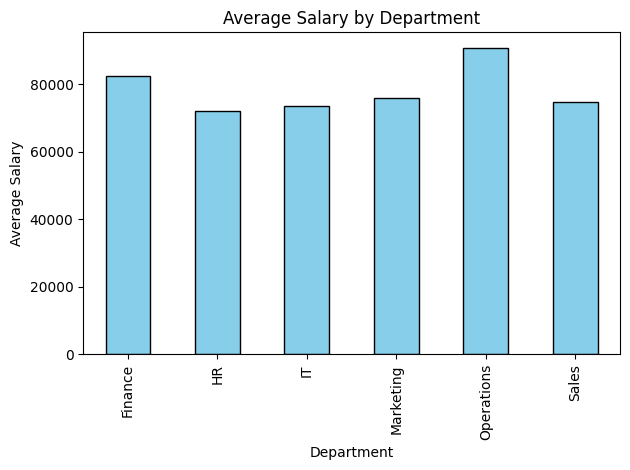
\includegraphics[width=0.82\textwidth,height=0.42\textheight,keepaspectratio]{figs/e1_2_0.png}\caption{Average Salary by Department}\end{figure}
\Needspace{14\baselineskip}\paragraph{Output 3: dept\_counts = df['Department'].value\_counts()}\mbox{}\\[-1ex]
\begin{Verbatim}[commandchars=\\\{\},breaklines=true,breakanywhere=true,fontsize=\scriptsize,frame=leftline,framesep=2mm,rulecolor=\color{gray}]
Number of employees in each department:

Department
HR            21
Marketing     20
IT            18
Operations    16
Sales         13
Finance       12
Name: count, dtype: int64
\end{Verbatim}
\Needspace{14\baselineskip}\paragraph{Output 4: df['Gender'].value\_counts().plot(kind='pie', autopct='\%1.1f\%\%', starta}\mbox{}\\[-1ex]
\begin{figure}[H]\centering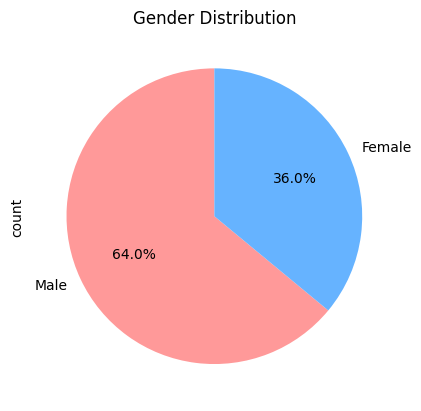
\includegraphics[width=0.82\textwidth,height=0.42\textheight,keepaspectratio]{figs/e1_4_0.png}\caption{Gender Distribution}\end{figure}
\Needspace{14\baselineskip}\paragraph{Output 5: df['Salary'].plot(kind='hist', bins=15, color='lightgreen', edgecolor=}\mbox{}\\[-1ex]
\begin{figure}[H]\centering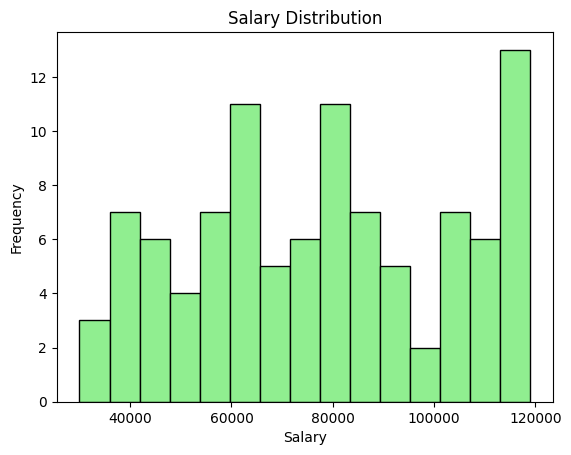
\includegraphics[width=0.82\textwidth,height=0.42\textheight,keepaspectratio]{figs/e1_5_0.png}\caption{Salary Distribution}\end{figure}
\Needspace{14\baselineskip}\paragraph{Output 6: plt.figure(figsize=(8, 5))}\mbox{}\\[-1ex]
\begin{figure}[H]\centering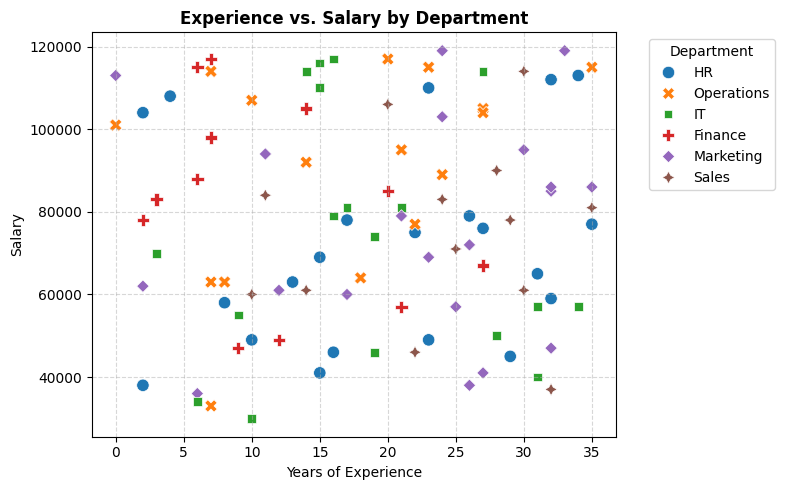
\includegraphics[width=0.82\textwidth,height=0.42\textheight,keepaspectratio]{figs/e1_6_0.png}\caption{Experience vs. Salary by Department}\end{figure}
\Needspace{14\baselineskip}\paragraph{Output 7: top\_10\_earners = df.nlargest(10, 'Salary')}\mbox{}\\[-1ex]
\begin{Verbatim}[commandchars=\\\{\},breaklines=true,breakanywhere=true,fontsize=\scriptsize,frame=leftline,framesep=2mm,rulecolor=\color{gray}]
Top 10 Employees with Highest Salary:

   Employee_ID       Name  Department  Age  Gender  Salary  Experience_Years
85        E086     Omar86   Marketing   58    Male  119000                24
87        E088    Diana88   Marketing   36    Male  119000                33
14        E015    Ishan15  Operations   57    Male  117000                20
22        E023    Rahul23     Finance   57    Male  117000                 7
58        E059     Neha59          IT   43    Male  117000                16
48        E049  Charlie49          IT   26    Male  116000                15
31        E032   George32  Operations   41  Female  115000                23
55        E056    Sneha56  Operations   41    Male  115000                35
64        E065      Bob65     Finance   35    Male  115000                 6
9         E010   Vikram10          IT   26    Male  114000                14
\end{Verbatim}
\Needspace{14\baselineskip}\paragraph{Output 8: max\_salary\_dept = df.groupby('Department')['Salary'].max()}\mbox{}\\[-1ex]
\begin{Verbatim}[commandchars=\\\{\},breaklines=true,breakanywhere=true,fontsize=\scriptsize,frame=leftline,framesep=2mm,rulecolor=\color{gray}]
Highest Salary in Each Department:

Department
Finance       117000
HR            113000
IT            117000
Marketing     119000
Operations    117000
Sales         114000
Name: Salary, dtype: int64
\end{Verbatim}
\Needspace{14\baselineskip}\paragraph{Output 9: avg\_salary = df['Salary'].mean()}\mbox{}\\[-1ex]
\begin{Verbatim}[commandchars=\\\{\},breaklines=true,breakanywhere=true,fontsize=\scriptsize,frame=leftline,framesep=2mm,rulecolor=\color{gray}]
Overall Average Salary: 77760.00

Employees earning more than the average:

   Employee_ID       Name  Department  Age  Gender  Salary  Experience_Years
1         E002     Diana2  Operations   56    Male  105000                27
3         E004      Neha4          HR   57    Male  113000                34
7         E008      Neha8     Finance   24  Female   98000                 7
8         E009     Mohan9          HR   57  Female  110000                23
9         E010   Vikram10          IT   26    Male  114000                14
10        E011    Julia11          HR   36    Male   78000                17
12        E013   George13  Operations   39    Male  107000                10
13        E014    Sneha14  Operations   37    Male   89000                24
14        E015    Ishan15  Operations   57    Male  117000                20
15        E016      Bob16          IT   24  Female   81000                17
18        E019     Hina19  Operations   57  Female  104000                27
21        E022    Nisha22       Sales   26  Female   78000                29
22        E023    Rahul23     Finance   57    Male  117000                 7
24        E025    Farah25   Marketing   22  Female   94000                11
26        E027    Farah27       Sales   55    Male  106000                20
29        E030  Charlie30       Sales   30    Male  114000                30
31        E032   George32  Operations   41  Female  115000                23
33        E034  Charlie34     Finance   23    Male  105000                14
37        E038    Nisha38          IT   28    Male  114000                27
40        E041   George41       Sales   50    Male   84000                11
41        E042    Ishan42   Marketing   37    Male   86000                35
44        E045      Bob45          IT   46    Male   79000                16
48        E049  Charlie49          IT   26    Male  116000                15
49        E050    Mohan50          HR   58    Male  104000                 2
52        E053     Omar53     Finance   26    Male   88000                 6
55        E056    Sneha56  Operations   41    Male  115000                35
58        E059     Neha59          IT   43    Male  117000                16
61        E062    Farah62  Operations   50  Female  101000                 0
64        E065      Bob65     Finance   35    Male  115000                 6
67        E068     Hina68     Finance   32    Male   78000                 2
69        E070     Hina70          IT   23    Male   81000                21
70        E071    Ishan71          HR   39  Female  112000                32
73        E074     Neha74   Marketing   44  Female   85000                32
76        E077  Charlie77  Operations   43  Female  114000                 7
78        E079    Julia79       Sales   30    Male   83000                24
79        E080    Farah80       Sales   58  Female   81000                35
80        E081    Alice81     Finance   40    Male   85000                20
81        E082     Omar82   Marketing   50    Male   95000                30
82        E083    Farah83  Operations   27  Female   95000                21
84        E085    Alice85          HR   37  Female  108000                 4
... [output truncated for length]
\end{Verbatim}
\Needspace{14\baselineskip}\paragraph{Output 10: avg\_exp\_dept = df.groupby('Department')['Experience\_Years'].mean()}\mbox{}\\[-1ex]
\begin{Verbatim}[commandchars=\\\{\},breaklines=true,breakanywhere=true,fontsize=\scriptsize,frame=leftline,framesep=2mm,rulecolor=\color{gray}]
Average Years of Experience by Department:

Department
Finance       11.166667
HR            19.809524
IT            18.388889
Marketing     21.900000
Operations    16.875000
Sales         23.846154
Name: Experience_Years, dtype: float64
\end{Verbatim}
\Needspace{14\baselineskip}\paragraph{Output 11: df['Age'].plot(kind='hist', bins=10, color='coral', edgecolor='black')}\mbox{}\\[-1ex]
\begin{figure}[H]\centering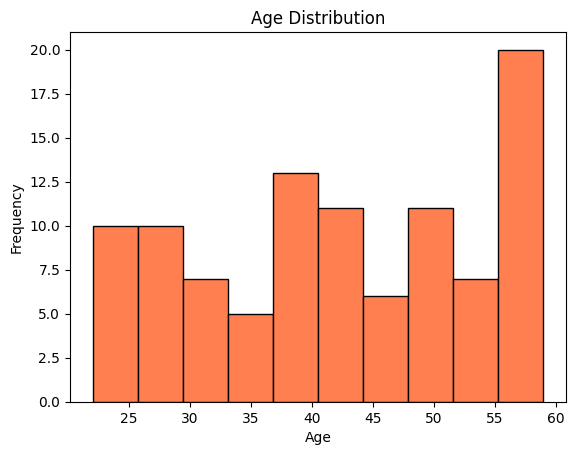
\includegraphics[width=0.82\textwidth,height=0.42\textheight,keepaspectratio]{figs/e1_11_0.png}\caption{Age Distribution}\end{figure}
\textbf{Observations.}

\begin{itemize}
\tightlist
\item
  Headcount by department is HR 21, Marketing 20, IT 18, Operations 16, Sales 13 and Finance 12, so HR and Marketing are the largest groups.
\item
  The overall average salary is 77,760. The highest salary in the company is 119,000, reached by two Marketing employees; the highest salary per department ranges from 113,000 (HR) to 119,000 (Marketing).
\item
  Average experience differs noticeably across departments, from about 11.2 years in Finance to about 23.8 years in Sales, with Marketing at about 21.9 years.
\item
  The experience-versus-salary scatter plot allows the relationship between seniority and pay to be inspected department by department.
\end{itemize}


\section{Conclusion}
The experiment showed how a few lines of pandas and seaborn can summarise a dataset's structure, group-level differences and distributions. The dataset is clean (no missing values), and the departmental summaries provide a clear picture of headcount, pay and experience. The same inspect-then-summarise workflow is reused for the text corpora in the following experiments.


\chapter{Experiment 2: Basic Text Preprocessing, Tokenization and Stopword Removal}
\section{Abstract}
This experiment covers the first stage of any NLP pipeline: cleaning raw text, splitting it into sentences and words with three different tools (NLTK, spaCy and pure regular expressions), and removing stopwords with NLTK's English list. Each step is applied to a supplied text file and the intermediate results are printed so that the effect of every transformation can be checked.


\section{Aim}
To clean and normalise raw text, to compare sentence and word tokenization across NLTK, spaCy and regex, and to filter stopwords from a tokenized text.


\section{Objectives}
\begin{itemize}
\item Count and remove uppercase letters, punctuation types, numbers and extra whitespace from a text.
\item Tokenize text into sentences and words using NLTK, spaCy and regular expressions.
\item Identify and remove English stopwords using NLTK.
\end{itemize}

\section{Description and Theoretical Background}
Raw text contains variation that is irrelevant to many tasks, such as case, punctuation and spacing. Normalisation reduces this variation. \textbf{Tokenization} splits text into units; sentence tokenization finds sentence boundaries, and word tokenization separates words and punctuation. Rule-based tokenizers such as a regex split are fast but need hand-written rules, while library tokenizers such as NLTK's Punkt model and spaCy's tokenizer encode language-specific rules. \textbf{Stopwords} are very frequent function words (for example \emph{the}, \emph{is}, \emph{of}) that carry little content for tasks such as retrieval or topic analysis, so they are often removed to shrink the vocabulary.


\section{Data Understanding}
Three small plain-text files were used: \texttt{2.1\_text\_data.txt} for cleaning, \texttt{2.2\_tokenization\_data.txt} for tokenization and \texttt{2.3\_clean\_data.txt} for stopword removal. All three are short English passages about natural language processing.


\section{Description of the Implemented Code}
\emph{Cleaning} lowercases the text after counting capital letters, builds the set of punctuation characters present, removes them with \texttt{str.translate}, finds numbers with \texttt{re.findall} before deleting them, and collapses repeated whitespace with \texttt{re.sub}. \emph{Tokenization} is implemented three times: NLTK (\texttt{sent\_tokenize}, \texttt{word\_tokenize}), spaCy (a blank English pipeline with the rule-based \texttt{sentencizer}) and regex (\texttt{re.split} on sentence-ending punctuation and \texttt{re.findall} for words and punctuation marks). \emph{Stopword removal} tokenizes the text, then splits tokens into stopwords and filtered tokens using NLTK's English stopword list.


\section{Implemented Code}
\Needspace{8\baselineskip}\paragraph{Listing 1: Read the dataset}\mbox{}\\[-1ex]
\begin{Verbatim}[commandchars=\\\{\},breaklines=true,breakanywhere=true,fontsize=\scriptsize,frame=leftline,framesep=2mm,rulecolor=\color{gray}]
import re
import string

# Read the dataset
with open("2.1_text_data (1).txt", "r") as file:
    text = file.read()

# 1. Count uppercase letters and convert to lowercase
uppercase = sum(1 for ch in text if ch.isupper())
text = text.lower()

# 2. Count different punctuation types and remove punctuation
punctuations = set(ch for ch in text if ch in string.punctuation)
text = text.translate(str.maketrans("", "", string.punctuation))

# 3. Count numbers and remove them
numbers = re.findall(r'\textbackslash{}d+', text)
text = re.sub(r'\textbackslash{}d+', '', text)

# 4. Count extra whitespace and remove it
extra_whitespace = len(text) - len(re.sub(r'\textbackslash{}s+', ' ', text))
text = re.sub(r'\textbackslash{}s+', ' ', text).strip()

# 5. Display results
print("Uppercase letters:", uppercase)
print("Different punctuation types:", len(punctuations))
print("Numbers:", len(numbers))
print("Extra whitespace:", extra_whitespace)

print("\textbackslash{}nCleaned Text:")
print(text)
\end{Verbatim}
\Needspace{8\baselineskip}\paragraph{Listing 2: Read the dataset}\mbox{}\\[-1ex]
\begin{Verbatim}[commandchars=\\\{\},breaklines=true,breakanywhere=true,fontsize=\scriptsize,frame=leftline,framesep=2mm,rulecolor=\color{gray}]
import nltk

nltk.download('punkt')
nltk.download('punkt_tab')

# Read the dataset
with open("2.2_tokenization_data (1).txt", "r") as file:
    text = file.read()

# Sentence tokenization
sentences = nltk.sent_tokenize(text)

# Word tokenization
words = nltk.word_tokenize(text)

print("SENTENCES:")
for sentence in sentences:
    print(sentence)

print("\textbackslash{}nWORDS:")
print(words)
\end{Verbatim}
\Needspace{8\baselineskip}\paragraph{Listing 3: Create a blank English pipeline}\mbox{}\\[-1ex]
\begin{Verbatim}[commandchars=\\\{\},breaklines=true,breakanywhere=true,fontsize=\scriptsize,frame=leftline,framesep=2mm,rulecolor=\color{gray}]
import spacy

# Create a blank English pipeline
nlp = spacy.blank("en")
nlp.add_pipe("sentencizer")

# Read the dataset
with open("2.2_tokenization_data (1).txt", "r") as file:
    text = file.read()

doc = nlp(text)

# Sentence tokenization
print("SENTENCES:")
for sentence in doc.sents:
    print(sentence.text)

# Word tokenization
print("\textbackslash{}nWORDS:")
for token in doc:
    print(token.text)
\end{Verbatim}
\Needspace{8\baselineskip}\paragraph{Listing 4: Read the dataset}\mbox{}\\[-1ex]
\begin{Verbatim}[commandchars=\\\{\},breaklines=true,breakanywhere=true,fontsize=\scriptsize,frame=leftline,framesep=2mm,rulecolor=\color{gray}]
import re

# Read the dataset
with open("2.2_tokenization_data (1).txt", "r") as file:
    text = file.read()

# Sentence tokenization
sentences = re.split(r'(?<=[.!?])\textbackslash{}s+', text.strip())

# Word tokenization
words = re.findall(r'\textbackslash{}w+|[^\textbackslash{}w\textbackslash{}s]', text)

print("SENTENCES:")
for sentence in sentences:
    print(sentence)

print("\textbackslash{}nWORDS:")
print(words)
\end{Verbatim}
\Needspace{8\baselineskip}\paragraph{Listing 5: Read the dataset}\mbox{}\\[-1ex]
\begin{Verbatim}[commandchars=\\\{\},breaklines=true,breakanywhere=true,fontsize=\scriptsize,frame=leftline,framesep=2mm,rulecolor=\color{gray}]
import nltk
from nltk.corpus import stopwords

nltk.download('stopwords')

# Read the dataset
with open("2.3_clean_data (1).txt", "r") as file:
    text = file.read()

# Tokenize the text
tokens = nltk.word_tokenize(text)

# Get English stop words
stop_words = set(stopwords.words('english'))

# Separate stop words and filtered tokens
found_stop_words = [word for word in tokens if word.lower() in stop_words]
filtered_tokens = [word for word in tokens if word.lower() not in stop_words]

print("ORIGINAL TOKENS:")
print(tokens)

print("\textbackslash{}nSTOP WORDS:")
print(found_stop_words)

print("\textbackslash{}nFILTERED TOKENS:")
print(filtered_tokens)
\end{Verbatim}

\section{Results and Observations}
\Needspace{14\baselineskip}\paragraph{Output 1: Read the dataset}\mbox{}\\[-1ex]
\begin{Verbatim}[commandchars=\\\{\},breaklines=true,breakanywhere=true,fontsize=\scriptsize,frame=leftline,framesep=2mm,rulecolor=\color{gray}]
Uppercase letters: 32
Different punctuation types: 6
Numbers: 3
Extra whitespace: 12

Cleaned Text:
natural language processing nlp is a branch of artificial intelligence it helps computers understand and process human language in nlp is used in many applications such as chatbots machine translation sentiment analysis and text summarization text preprocessing is an important step in nlp it include ...
\end{Verbatim}
\Needspace{14\baselineskip}\paragraph{Output 2: Read the dataset}\mbox{}\\[-1ex]
\begin{Verbatim}[commandchars=\\\{\},breaklines=true,breakanywhere=true,fontsize=\scriptsize,frame=leftline,framesep=2mm,rulecolor=\color{gray}]
SENTENCES:
Natural Language Processing (NLP) is a fascinating field of Artificial Intelligence.
It enables computers to understand human language.
NLP is used in many real-world applications, such as chatbots, machine translation, sentiment analysis, and text summarization.
Text tokenization is one of the first steps in NLP.
Sentence tokenization divides a paragraph into individual sentences.
Word tokenization divides each sentence into individual words and tokens.
For example, a chatbot receives thousands of messages every day.
The system processes these messages and identifies useful information.
This information can then be used to provide better responses to users.

WORDS:
['Natural', 'Language', 'Processing', '(', 'NLP', ')', 'is', 'a', 'fascinating', 'field', 'of', 'Artificial', 'Intelligence', '.', 'It', 'enables', 'computers', 'to', 'understand', 'human', 'language', '.', 'NLP', 'is', 'used', 'in', 'many', 'real-world', 'applications', ',', 'such', 'as', 'chatbots ...
\end{Verbatim}
\Needspace{14\baselineskip}\paragraph{Output 3: Create a blank English pipeline}\mbox{}\\[-1ex]
\begin{Verbatim}[commandchars=\\\{\},breaklines=true,breakanywhere=true,fontsize=\scriptsize,frame=leftline,framesep=2mm,rulecolor=\color{gray}]
SENTENCES:
Natural Language Processing (NLP) is a fascinating field of Artificial Intelligence.
It enables computers to understand human language.
NLP is used in many real-world applications, such as chatbots, machine translation, sentiment analysis, and text summarization.

Text tokenization is one of the first steps in NLP.
Sentence tokenization divides a paragraph into individual sentences.
Word tokenization divides each sentence into individual words and tokens.

For example, a chatbot receives thousands of messages every day.
The system processes these messages and identifies useful information.
This information can then be used to provide better responses to users.

WORDS:
Natural
Language
Processing
(
NLP
)
is
a
fascinating
field
of
Artificial
Intelligence
.
It
enables
computers
to
understand
human
language
.
NLP
is
used
in
many
real
-
world
applications
... [output truncated for length]
\end{Verbatim}
\Needspace{14\baselineskip}\paragraph{Output 4: Read the dataset}\mbox{}\\[-1ex]
\begin{Verbatim}[commandchars=\\\{\},breaklines=true,breakanywhere=true,fontsize=\scriptsize,frame=leftline,framesep=2mm,rulecolor=\color{gray}]
SENTENCES:
Natural Language Processing (NLP) is a fascinating field of Artificial Intelligence.
It enables computers to understand human language.
NLP is used in many real-world applications, such as chatbots, machine translation, sentiment analysis, and text summarization.
Text tokenization is one of the first steps in NLP.
Sentence tokenization divides a paragraph into individual sentences.
Word tokenization divides each sentence into individual words and tokens.
For example, a chatbot receives thousands of messages every day.
The system processes these messages and identifies useful information.
This information can then be used to provide better responses to users.

WORDS:
['Natural', 'Language', 'Processing', '(', 'NLP', ')', 'is', 'a', 'fascinating', 'field', 'of', 'Artificial', 'Intelligence', '.', 'It', 'enables', 'computers', 'to', 'understand', 'human', 'language', '.', 'NLP', 'is', 'used', 'in', 'many', 'real', '-', 'world', 'applications', ',', 'such', 'as', ' ...
\end{Verbatim}
\Needspace{14\baselineskip}\paragraph{Output 5: Read the dataset}\mbox{}\\[-1ex]
\begin{Verbatim}[commandchars=\\\{\},breaklines=true,breakanywhere=true,fontsize=\scriptsize,frame=leftline,framesep=2mm,rulecolor=\color{gray}]
ORIGINAL TOKENS:
['Natural', 'Language', 'Processing', 'is', 'an', 'important', 'field', 'of', 'Artificial', 'Intelligence', '.', 'It', 'is', 'used', 'in', 'many', 'applications', 'such', 'as', 'chatbots', ',', 'machine', 'translation', ',', 'sentiment', 'analysis', ',', 'and', 'text', 'summarization', '.', 'The', ' ...

STOP WORDS:
['is', 'an', 'of', 'It', 'is', 'in', 'such', 'as', 'and', 'The', 'of', 'is', 'to', 'to', 'and', 'A', 'can', 'a', 'of', 'in', 'a', 'of', 'The', 'of', 'is', 'of', 'the', 'in', 'are', 'such', 'as', 'the', 'is', 'a', 'an', 'in', 'of', 'and', 'to', 'for', 'on', 'with', 'from', 'by', 'this', 'that', 'and' ...

FILTERED TOKENS:
['Natural', 'Language', 'Processing', 'important', 'field', 'Artificial', 'Intelligence', '.', 'used', 'many', 'applications', 'chatbots', ',', 'machine', 'translation', ',', 'sentiment', 'analysis', ',', 'text', 'summarization', '.', 'main', 'purpose', 'NLP', 'enable', 'computers', 'understand', 'p ...
\end{Verbatim}
\textbf{Observations.}

\begin{itemize}
\tightlist
\item
  The cleaning step counted 32 uppercase letters, 6 distinct punctuation types, 3 numbers and 12 extra whitespace characters, and produced a fully lowercase, punctuation-free text with single spaces.
\item
  NLTK, spaCy and the regex approach all recover the same sentences for this clean passage. The regex word pattern also keeps each punctuation mark as its own token, as NLTK does.
\item
  After stopword removal, content words such as \emph{Natural}, \emph{Language}, \emph{Processing}, \emph{chatbots}, \emph{machine} and \emph{translation} remain, while function words such as \emph{is}, \emph{of} and \emph{the} are removed. Punctuation tokens survive because they are not in the stopword list; they would need a separate filter.
\end{itemize}


\section{Conclusion}
Basic cleaning, tokenization and stopword removal turn raw text into a consistent token sequence. The three tokenizers behave similarly on well-formed text, but the library tools handle more edge cases than a hand-written regex. Stopword removal shrinks the token list substantially, but punctuation has to be removed separately.


\chapter{Experiment 3: Stemming, Lemmatization and Regular-Expression Information Extraction}
\section{Abstract}
This experiment compares two ways of reducing words to a base form, the rule-based Porter stemmer and the dictionary-based WordNet lemmatizer, and uses regular expressions to extract emails, URLs, mobile numbers, hashtags and mentions from unstructured text.


\section{Aim}
To apply stemming and lemmatization to word lists, observe their differences, and extract structured information from text using regular expressions.


\section{Objectives}
\begin{itemize}
\item Apply the Porter stemmer to a list of inflected words.
\item Apply the WordNet lemmatizer with and without part-of-speech information.
\item Write regular expressions for emails, URLs, mobile numbers, hashtags and mentions.
\end{itemize}

\section{Description and Theoretical Background}
\textbf{Stemming} removes suffixes by rules; the Porter algorithm is fast but can produce non-words (\emph{studies} becomes \emph{studi}). \textbf{Lemmatization} looks words up in a lexicon (WordNet) and returns a valid dictionary form, but it needs the part of speech to treat verbs, nouns and adjectives correctly. \textbf{Regular expressions} describe patterns over characters and can be compiled to finite-state automata, which makes them an efficient way to extract strings with a regular shape such as emails and hashtags.


\section{Data Understanding}
The stemming list had eight words (playing, played, plays, studies, studying, connected, connection, computers). The lemmatization list had fourteen words including irregular forms (ran, mice, went, ate, better, children). The extraction text was a short workshop announcement containing emails, links, phone numbers, hashtags and mentions.


\section{Description of the Implemented Code}
Stemming uses \texttt{PorterStemmer.stem}. Lemmatization uses \texttt{WordNetLemmatizer.lemmatize}, first with the default (noun) tag and then with an explicit POS tag per word (\texttt{n}, \texttt{v}, \texttt{a}). Information extraction uses \texttt{re.findall} with a separate pattern for each of the five entity types.


\section{Implemented Code}
\Needspace{8\baselineskip}\paragraph{Listing 1: nltk.download('punkt')}\mbox{}\\[-1ex]
\begin{Verbatim}[commandchars=\\\{\},breaklines=true,breakanywhere=true,fontsize=\scriptsize,frame=leftline,framesep=2mm,rulecolor=\color{gray}]
import nltk
from nltk.stem import PorterStemmer

nltk.download('punkt')

stemmer = PorterStemmer()

words = [
    "playing", "played", "plays", "studies",
    "studying", "connected", "connection", "computers"
]

print("Original Word -> Stem")
print("-" * 30)

for word in words:
    stem = stemmer.stem(word)
    print(f"\textbraceleft{}word:15\textbraceright{} -> \textbraceleft{}stem\textbraceright{}")
\end{Verbatim}
\Needspace{8\baselineskip}\paragraph{Listing 2: nltk.download('wordnet')}\mbox{}\\[-1ex]
\begin{Verbatim}[commandchars=\\\{\},breaklines=true,breakanywhere=true,fontsize=\scriptsize,frame=leftline,framesep=2mm,rulecolor=\color{gray}]
from nltk.stem import WordNetLemmatizer

nltk.download('wordnet')
nltk.download('omw-1.4')

lemmatizer = WordNetLemmatizer()

words = [
    "cats", "dogs", "running", "runs", "ran",
    "studies", "studying", "better", "children",
    "mice", "went", "ate", "leaves", "caring"
]

print("Original Word -> Lemma")
print("-" * 30)

for word in words:
    lemma = lemmatizer.lemmatize(word)
    print(f"\textbraceleft{}word:15\textbraceright{} -> \textbraceleft{}lemma\textbraceright{}")
\end{Verbatim}
\Needspace{8\baselineskip}\paragraph{Listing 3: words = \{}\mbox{}\\[-1ex]
\begin{Verbatim}[commandchars=\\\{\},breaklines=true,breakanywhere=true,fontsize=\scriptsize,frame=leftline,framesep=2mm,rulecolor=\color{gray}]
words = \textbraceleft{}
    "cats": "n",
    "dogs": "n",
    "running": "v",
    "runs": "v",
    "ran": "v",
    "studies": "v",
    "studying": "v",
    "better": "a",
    "children": "n",
    "mice": "n",
    "went": "v",
    "ate": "v",
    "leaves": "n",
    "caring": "v"
\textbraceright{}

print("Original Word -> Lemma")
print("-" * 30)

for word, pos in words.items():
    lemma = lemmatizer.lemmatize(word, pos=pos)
    print(f"\textbraceleft{}word:15\textbraceright{} -> \textbraceleft{}lemma\textbraceright{}")
\end{Verbatim}
\Needspace{8\baselineskip}\paragraph{Listing 4: Experiment 3.3: Extract information using Regular Expressions}\mbox{}\\[-1ex]
\begin{Verbatim}[commandchars=\\\{\},breaklines=true,breakanywhere=true,fontsize=\scriptsize,frame=leftline,framesep=2mm,rulecolor=\color{gray}]
# Experiment 3.3: Extract information using Regular Expressions

import re

# Given input text
text = """
Welcome to the Natural Language Processing workshop! For more information, visit
https://www.nlpworkshop.com or www.python.org. You can contact the coordinator at
nlpworkshop@gmail.com or support@python.org. For registration, call +91-9876543210 or
9123456789. Follow us on social media @NLPWorkshop and @PythonLearner. Share your
experience using #NLP, #Python, and #MachineLearning. You can also visit
https://github.com/NLPWorkshop for the latest updates.
"""

# 1. Extract Email Addresses
emails = re.findall(
    r'[A-Za-z0-9._%+-]+@[A-Za-z0-9.-]+\textbackslash{}.[A-Za-z]\textbraceleft{}2,\textbraceright{}',
    text
)

# 2. Extract URLs
urls = re.findall(
    r'(?:https?://|www\textbackslash{}.)[A-Za-z0-9.-]+(?:/[A-Za-z0-9._~:/?#\textbackslash{}[\textbackslash{}]@!$&\textbackslash{}'()*+,;=%-]*)?',
    text
)

# 3. Extract Mobile Numbers
mobile_numbers = re.findall(
    r'(?:\textbackslash{}+91[-\textbackslash{}s]?)?[6-9]\textbackslash{}d\textbraceleft{}9\textbraceright{}',
    text
)

# 4. Extract Hashtags
hashtags = re.findall(
    r'#[A-Za-z0-9_]+',
    text
)

# 5. Extract Mentions
mentions = re.findall(
    r'@[A-Za-z0-9_]+',
    text
)

# Display results
print("EMAIL ADDRESSES:")
for item in emails:
    print(item)

print("\textbackslash{}nURLS:")
for item in urls:
    print(item)

print("\textbackslash{}nMOBILE NUMBERS:")
for item in mobile_numbers:
    print(item)

print("\textbackslash{}nHASHTAGS:")
for item in hashtags:
    print(item)

print("\textbackslash{}nMENTIONS:")
for item in mentions:
    print(item)
\end{Verbatim}

\section{Results and Observations}
\Needspace{14\baselineskip}\paragraph{Output 1: nltk.download('punkt')}\mbox{}\\[-1ex]
\begin{Verbatim}[commandchars=\\\{\},breaklines=true,breakanywhere=true,fontsize=\scriptsize,frame=leftline,framesep=2mm,rulecolor=\color{gray}]
Original Word -> Stem
------------------------------
playing         -> play
played          -> play
plays           -> play
studies         -> studi
studying        -> studi
connected       -> connect
connection      -> connect
computers       -> comput
\end{Verbatim}
\Needspace{14\baselineskip}\paragraph{Output 2: nltk.download('wordnet')}\mbox{}\\[-1ex]
\begin{Verbatim}[commandchars=\\\{\},breaklines=true,breakanywhere=true,fontsize=\scriptsize,frame=leftline,framesep=2mm,rulecolor=\color{gray}]
Original Word -> Lemma
------------------------------
cats            -> cat
dogs            -> dog
running         -> running
runs            -> run
ran             -> ran
studies         -> study
studying        -> studying
better          -> better
children        -> child
mice            -> mouse
went            -> went
ate             -> ate
leaves          -> leaf
caring          -> caring
\end{Verbatim}
\Needspace{14\baselineskip}\paragraph{Output 3: words = \{}\mbox{}\\[-1ex]
\begin{Verbatim}[commandchars=\\\{\},breaklines=true,breakanywhere=true,fontsize=\scriptsize,frame=leftline,framesep=2mm,rulecolor=\color{gray}]
Original Word -> Lemma
------------------------------
cats            -> cat
dogs            -> dog
running         -> run
runs            -> run
ran             -> run
studies         -> study
studying        -> study
better          -> good
children        -> child
mice            -> mouse
went            -> go
ate             -> eat
leaves          -> leaf
caring          -> care
\end{Verbatim}
\Needspace{14\baselineskip}\paragraph{Output 4: Experiment 3.3: Extract information using Regular Expressions}\mbox{}\\[-1ex]
\begin{Verbatim}[commandchars=\\\{\},breaklines=true,breakanywhere=true,fontsize=\scriptsize,frame=leftline,framesep=2mm,rulecolor=\color{gray}]
EMAIL ADDRESSES:
nlpworkshop@gmail.com
support@python.org

URLS:
https://www.nlpworkshop.com
www.python.org.
https://github.com/NLPWorkshop

MOBILE NUMBERS:
+91-9876543210
9123456789

HASHTAGS:
#NLP
#Python
#MachineLearning

MENTIONS:
@gmail
@python
@NLPWorkshop
@PythonLearner
\end{Verbatim}
\textbf{Observations.}

\begin{itemize}
\tightlist
\item
  The stemmer maps \emph{playing}, \emph{played} and \emph{plays} to \emph{play} and \emph{connected} and \emph{connection} to \emph{connect}, but reduces \emph{studies} and \emph{studying} to the non-word \emph{studi} and \emph{computers} to \emph{comput}.
\item
  Without POS information the lemmatizer treats every word as a noun, so \emph{running} and \emph{ran} are unchanged. With the correct tags it returns \emph{run} for both, \emph{good} for \emph{better} and \emph{mouse} for \emph{mice}.
\item
  The regular expressions found two emails, three URLs, two mobile numbers, three hashtags and four mentions. Two imperfections are visible: the URL pattern kept a trailing full stop (\emph{www.python.org.}), and the mention pattern also matched the domain parts of the two email addresses (\emph{@gmail}, \emph{@python}). Both could be fixed by tightening the patterns.
\end{itemize}


\section{Conclusion}
Stemming is quick but crude, while lemmatization gives valid words but depends on correct POS tags. Regular expressions extract well-structured strings reliably, though simple patterns can produce false positives and need refinement for real data.


\chapter{Experiment 4: Term Frequency, Named Entity Recognition and TF-IDF from Scratch}
\section{Abstract}
This experiment computes term frequencies on a text corpus with a toolkit-assisted pipeline (spaCy) and with pure Python, performs named entity recognition with spaCy, and implements TF, DF, IDF and TF-IDF from scratch for a small multi-document collection.


\section{Aim}
To compute and compare term-frequency tables using a toolkit and pure Python, to extract named entities, and to implement TF-IDF weighting without an NLP library.


\section{Objectives}
\begin{itemize}
\item Count word frequencies, save the (Term, Frequency) table to CSV and display the top ten terms.
\item Run named entity recognition with spaCy and save the entities.
\item Implement the pure-Python term-frequency counter and verify it matches the toolkit result.
\item Compute TF, DF, IDF and TF-IDF for multiple documents and list the top ten TF-IDF terms of each.
\end{itemize}

\section{Description and Theoretical Background}
\textbf{Term frequency} counts how often a term occurs. \textbf{Document frequency} (DF) is the number of documents containing a term, and \textbf{inverse document frequency} is \(IDF(t)=\log\frac{N}{DF(t)}\) where \(N\) is the number of documents. TF-IDF is the product \(TF(t,d)\times IDF(t)\), with \(TF(t,d)\) the count of \(t\) in \(d\) divided by the length of \(d\); it rewards terms that are frequent in one document but rare across the collection. \textbf{Named entity recognition} labels spans of text such as organisations, persons and dates using a trained statistical model.


\section{Data Understanding}
Parts 4.1 and 4.2 used the same input text file with 750 unique terms. Part 4.3 used three short text documents (\texttt{Document\_1}, \texttt{Document\_2}, \texttt{Document\_3}) with 9, 8 and 9 tokens after preprocessing.


\section{Data Preprocessing}
Text is lowercased and tokens are extracted with a regular expression that keeps alphanumeric words and internal hyphens or apostrophes. For TF-IDF the documents are lowercased, non-alphanumeric characters are replaced with spaces and the text is split on whitespace.


\section{Description of the Implemented Code}
Part 4.1 counts tokens with \texttt{collections.Counter}, writes the sorted table to CSV with pandas, and applies \texttt{en\_core\_web\_sm} to produce entities with their labels and descriptions. Part 4.2 repeats the count using only the standard library. Part 4.3 builds TF dictionaries per document, DF counts over the set of terms of each document, IDF with the natural logarithm, and TF-IDF as their product; the full table and the top-ten terms per document are exported as CSV files.


\section{Implemented Code}
\Needspace{8\baselineskip}\paragraph{Listing 1: Cell 3}\mbox{}\\[-1ex]
\begin{Verbatim}[commandchars=\\\{\},breaklines=true,breakanywhere=true,fontsize=\scriptsize,frame=leftline,framesep=2mm,rulecolor=\color{gray}]
!pip -q install spacy
!python -m spacy download en_core_web_sm
\end{Verbatim}
\Needspace{8\baselineskip}\paragraph{Listing 2: INPUT\_FILE\_41 = "/content/drive/MyDrive/4.1\_4.2\_input.txt"}\mbox{}\\[-1ex]
\begin{Verbatim}[commandchars=\\\{\},breaklines=true,breakanywhere=true,fontsize=\scriptsize,frame=leftline,framesep=2mm,rulecolor=\color{gray}]
INPUT_FILE_41 = "/content/drive/MyDrive/4.1_4.2_input.txt"

TF_CSV_41 = "/content/term_frequency_4_1.csv"
NER_CSV_41 = "/content/ner_results_4_1.csv"
\end{Verbatim}
\Needspace{8\baselineskip}\paragraph{Listing 3: with open(INPUT\_FILE\_41, "r", encoding="utf-8") as f:}\mbox{}\\[-1ex]
\begin{Verbatim}[commandchars=\\\{\},breaklines=true,breakanywhere=true,fontsize=\scriptsize,frame=leftline,framesep=2mm,rulecolor=\color{gray}]
import re
import csv
from collections import Counter

import pandas as pd
import spacy

with open(INPUT_FILE_41, "r", encoding="utf-8") as f:
    text_41 = f.read()

terms_41 = re.findall(r"\textbackslash{}b[a-zA-Z0-9]+(?:['-][a-zA-Z0-9]+)*\textbackslash{}b", text_41.lower())
freq_41 = Counter(terms_41)

tf_df_41 = pd.DataFrame(freq_41.items(), columns=["Term", "Frequency"])
tf_df_41 = tf_df_41.sort_values(
    by=["Frequency", "Term"], ascending=[False, True]
).reset_index(drop=True)

tf_df_41.to_csv(TF_CSV_41, index=False)

print(f"Total unique terms: \textbraceleft{}len(tf_df_41)\textbraceright{}")
print(f"TF output saved to: \textbraceleft{}TF_CSV_41\textbraceright{}")

print("\textbackslash{}nTop 10 most frequent terms:")
display(tf_df_41.head(10))
\end{Verbatim}
\Needspace{8\baselineskip}\paragraph{Listing 4: nlp = spacy.load("en\_core\_web\_sm")}\mbox{}\\[-1ex]
\begin{Verbatim}[commandchars=\\\{\},breaklines=true,breakanywhere=true,fontsize=\scriptsize,frame=leftline,framesep=2mm,rulecolor=\color{gray}]
nlp = spacy.load("en_core_web_sm")
doc = nlp(text_41)

entities_41 = [
    \textbraceleft{}
        "Entity": ent.text,
        "Label": ent.label_,
        "Description": spacy.explain(ent.label_) or ""
    \textbraceright{}
    for ent in doc.ents
]

ner_df_41 = pd.DataFrame(entities_41)

if ner_df_41.empty:
    print("No named entities were detected.")
else:
    display(ner_df_41)
    ner_df_41.to_csv(NER_CSV_41, index=False)
    print(f"NER output saved to: \textbraceleft{}NER_CSV_41\textbraceright{}")
\end{Verbatim}
\Needspace{8\baselineskip}\paragraph{Listing 5: INPUT\_FILE\_42 = "/content/drive/MyDrive/4.1\_4.2\_input.txt"}\mbox{}\\[-1ex]
\begin{Verbatim}[commandchars=\\\{\},breaklines=true,breakanywhere=true,fontsize=\scriptsize,frame=leftline,framesep=2mm,rulecolor=\color{gray}]
INPUT_FILE_42 = "/content/drive/MyDrive/4.1_4.2_input.txt"
TF_CSV_42 = "/content/term_frequency_4_2.csv"
\end{Verbatim}
\Needspace{8\baselineskip}\paragraph{Listing 6: with open(INPUT\_FILE\_42, "r", encoding="utf-8") as f:}\mbox{}\\[-1ex]
\begin{Verbatim}[commandchars=\\\{\},breaklines=true,breakanywhere=true,fontsize=\scriptsize,frame=leftline,framesep=2mm,rulecolor=\color{gray}]
import re
import csv
from collections import Counter

with open(INPUT_FILE_42, "r", encoding="utf-8") as f:
    text_42 = f.read()

words_42 = re.findall(r"\textbackslash{}b[a-zA-Z0-9]+(?:['-][a-zA-Z0-9]+)*\textbackslash{}b", text_42.lower())

frequency_42 = Counter(words_42)

rows_42 = sorted(frequency_42.items(), key=lambda x: (-x[1], x[0]))

with open(TF_CSV_42, "w", newline="", encoding="utf-8") as f:
    writer = csv.writer(f)
    writer.writerow(["Term", "Frequency"])
    writer.writerows(rows_42)

print(f"Total unique terms: \textbraceleft{}len(rows_42)\textbraceright{}")
print(f"TF output saved to: \textbraceleft{}TF_CSV_42\textbraceright{}")

print("\textbackslash{}nTop 10 most frequent terms:")
for term, count in rows_42[:10]:
    print(f"\textbraceleft{}term\textbraceright{}: \textbraceleft{}count\textbraceright{}")
\end{Verbatim}
\Needspace{8\baselineskip}\paragraph{Listing 7: tf\_df\_42 = pd.DataFrame(rows\_42, columns=["Term", "Frequency"])}\mbox{}\\[-1ex]
\begin{Verbatim}[commandchars=\\\{\},breaklines=true,breakanywhere=true,fontsize=\scriptsize,frame=leftline,framesep=2mm,rulecolor=\color{gray}]
tf_df_42 = pd.DataFrame(rows_42, columns=["Term", "Frequency"])
display(tf_df_42)
\end{Verbatim}
\Needspace{8\baselineskip}\paragraph{Listing 8: DATASET\_DIR\_43 = "/content/drive/MyDrive/Experiment\_4\_3\_Text\_Documents}\mbox{}\\[-1ex]
\begin{Verbatim}[commandchars=\\\{\},breaklines=true,breakanywhere=true,fontsize=\scriptsize,frame=leftline,framesep=2mm,rulecolor=\color{gray}]
DATASET_DIR_43 = "/content/drive/MyDrive/Experiment_4_3_Text_Documents"

OUTPUT_DIR_43 = "/content/tf_idf_outputs"

ALL_RESULTS_CSV_43 = f"\textbraceleft{}OUTPUT_DIR_43\textbraceright{}/tf_df_idf_tfidf_all.csv"
TOP10_CSV_43 = f"\textbraceleft{}OUTPUT_DIR_43\textbraceright{}/top10_tfidf_terms.csv"
\end{Verbatim}
\Needspace{8\baselineskip}\paragraph{Listing 9: os.makedirs(OUTPUT\_DIR\_43, exist\_ok=True)}\mbox{}\\[-1ex]
\begin{Verbatim}[commandchars=\\\{\},breaklines=true,breakanywhere=true,fontsize=\scriptsize,frame=leftline,framesep=2mm,rulecolor=\color{gray}]
import os
import re
import math
import pandas as pd
from collections import Counter

os.makedirs(OUTPUT_DIR_43, exist_ok=True)

doc_files_43 = sorted(
    os.path.join(DATASET_DIR_43, name)
    for name in os.listdir(DATASET_DIR_43)
    if name.lower().endswith(".txt")
)

if not doc_files_43:
    raise FileNotFoundError(
        f"No .txt files found in \textbraceleft{}DATASET_DIR_43\textbraceright{}. "
        "Upload your documents and update DATASET_DIR_43."
    )

print(f"Found \textbraceleft{}len(doc_files_43)\textbraceright{} document(s):")
for path in doc_files_43:
    print(" -", os.path.basename(path))
\end{Verbatim}
\Needspace{8\baselineskip}\paragraph{Listing 10: documents\_43 = \{\}}\mbox{}\\[-1ex]
\begin{Verbatim}[commandchars=\\\{\},breaklines=true,breakanywhere=true,fontsize=\scriptsize,frame=leftline,framesep=2mm,rulecolor=\color{gray}]
documents_43 = \textbraceleft{}\textbraceright{}

for path in doc_files_43:
    name = os.path.splitext(os.path.basename(path))[0]

    with open(path, "r", encoding="utf-8") as f:
        raw_text = f.read()

    text = raw_text.lower()

    text = re.sub(r"[^a-z0-9\textbackslash{}s]", " ", text)

    tokens = re.findall(r"\textbackslash{}b[a-z0-9]+\textbackslash{}b", text)

    documents_43[name] = tokens

print("\textbackslash{}nPreprocessed documents:")
for name, tokens in documents_43.items():
    print(f"\textbraceleft{}name\textbraceright{}: \textbraceleft{}len(tokens)\textbraceright{} tokens")
\end{Verbatim}
\Needspace{8\baselineskip}\paragraph{Listing 11: tf\_by\_doc = \{\}}\mbox{}\\[-1ex]
\begin{Verbatim}[commandchars=\\\{\},breaklines=true,breakanywhere=true,fontsize=\scriptsize,frame=leftline,framesep=2mm,rulecolor=\color{gray}]
tf_by_doc = \textbraceleft{}\textbraceright{}

for doc_name, tokens in documents_43.items():
    counts = Counter(tokens)
    total_terms = len(tokens)

    tf_by_doc[doc_name] = \textbraceleft{}
        term: count / total_terms
        for term, count in counts.items()
    \textbraceright{}

tf_rows = []
for doc_name, tf_values in tf_by_doc.items():
    for term, tf in tf_values.items():
        tf_rows.append(\textbraceleft{}
            "Document": doc_name,
            "Term": term,
            "TF": tf
        \textbraceright{})

tf_df = pd.DataFrame(tf_rows).sort_values(
    by=["Document", "TF", "Term"],
    ascending=[True, False, True]
).reset_index(drop=True)

print("TF values:")
display(tf_df)
\end{Verbatim}
\Needspace{8\baselineskip}\paragraph{Listing 12: num\_documents = len(documents\_43)}\mbox{}\\[-1ex]
\begin{Verbatim}[commandchars=\\\{\},breaklines=true,breakanywhere=true,fontsize=\scriptsize,frame=leftline,framesep=2mm,rulecolor=\color{gray}]
num_documents = len(documents_43)

df_counts = Counter()

for tokens in documents_43.values():
    for term in set(tokens):
        df_counts[term] += 1

df_df = pd.DataFrame(
    [\textbraceleft{}"Term": term, "DF": df\textbraceright{} for term, df in df_counts.items()]
).sort_values(
    by=["DF", "Term"], ascending=[False, True]
).reset_index(drop=True)

print("DF values:")
display(df_df)
\end{Verbatim}
\Needspace{8\baselineskip}\paragraph{Listing 13: idf\_df = df\_df.copy()}\mbox{}\\[-1ex]
\begin{Verbatim}[commandchars=\\\{\},breaklines=true,breakanywhere=true,fontsize=\scriptsize,frame=leftline,framesep=2mm,rulecolor=\color{gray}]
idf_df = df_df.copy()
idf_df["IDF"] = idf_df["DF"].apply(
    lambda df: math.log(num_documents / df)
)

print("IDF values:")
display(idf_df[["Term", "DF", "IDF"]])
\end{Verbatim}
\Needspace{8\baselineskip}\paragraph{Listing 14: idf\_lookup = dict(zip(idf\_df["Term"], idf\_df["IDF"]))}\mbox{}\\[-1ex]
\begin{Verbatim}[commandchars=\\\{\},breaklines=true,breakanywhere=true,fontsize=\scriptsize,frame=leftline,framesep=2mm,rulecolor=\color{gray}]
idf_lookup = dict(zip(idf_df["Term"], idf_df["IDF"]))

tfidf_rows = []

for doc_name, tf_values in tf_by_doc.items():
    for term, tf in tf_values.items():
        idf = idf_lookup[term]
        tfidf = tf * idf

        tfidf_rows.append(\textbraceleft{}
            "Document": doc_name,
            "Term": term,
            "TF": tf,
            "DF": df_counts[term],
            "IDF": idf,
            "TF-IDF": tfidf
        \textbraceright{})

tfidf_df = pd.DataFrame(tfidf_rows).sort_values(
    by=["Document", "TF-IDF", "Term"],
    ascending=[True, False, True]
).reset_index(drop=True)

print("TF, DF, IDF and TF-IDF:")
display(tfidf_df)
\end{Verbatim}
\Needspace{8\baselineskip}\paragraph{Listing 15: tfidf\_df.to\_csv(ALL\_RESULTS\_CSV\_43, index=False)}\mbox{}\\[-1ex]
\begin{Verbatim}[commandchars=\\\{\},breaklines=true,breakanywhere=true,fontsize=\scriptsize,frame=leftline,framesep=2mm,rulecolor=\color{gray}]
tfidf_df.to_csv(ALL_RESULTS_CSV_43, index=False)

print(f"Complete TF-IDF table saved to: \textbraceleft{}ALL_RESULTS_CSV_43\textbraceright{}")
\end{Verbatim}
\Needspace{8\baselineskip}\paragraph{Listing 16: top10\_rows = []}\mbox{}\\[-1ex]
\begin{Verbatim}[commandchars=\\\{\},breaklines=true,breakanywhere=true,fontsize=\scriptsize,frame=leftline,framesep=2mm,rulecolor=\color{gray}]
top10_rows = []

for doc_name in documents_43:
    top10 = (
        tfidf_df[tfidf_df["Document"] == doc_name]
        .sort_values(by=["TF-IDF", "Term"], ascending=[False, True])
        .head(10)
        .copy()
    )

    print(f"\textbackslash{}nTop 10 TF-IDF terms — \textbraceleft{}doc_name\textbraceright{}")
    display(top10[["Term", "TF", "DF", "IDF", "TF-IDF"]])

    for rank, (_, row) in enumerate(top10.iterrows(), start=1):
        top10_rows.append(\textbraceleft{}
            "Document": doc_name,
            "Rank": rank,
            "Term": row["Term"],
            "TF": row["TF"],
            "DF": row["DF"],
            "IDF": row["IDF"],
            "TF-IDF": row["TF-IDF"]
        \textbraceright{})

top10_df = pd.DataFrame(top10_rows)
top10_df.to_csv(TOP10_CSV_43, index=False)

print(f"Top-10 results saved to: \textbraceleft{}TOP10_CSV_43\textbraceright{}")
\end{Verbatim}

\section{Results and Observations}
\Needspace{14\baselineskip}\paragraph{Output 1: Cell 3}\mbox{}\\[-1ex]
\begin{Verbatim}[commandchars=\\\{\},breaklines=true,breakanywhere=true,fontsize=\scriptsize,frame=leftline,framesep=2mm,rulecolor=\color{gray}]
Collecting en-core-web-sm==3.8.0
  Downloading https://github.com/explosion/spacy-models/releases/download/en_core_web_sm-3.8.0/en_core_web_sm-3.8.0-py3-none-any.whl (12.8 MB)
[?25h Download and installation successful
You can now load the package via spacy.load('en_core_web_sm')
 Restart to reload dependencies
If you are in a Jupyter or Colab notebook, you may need to restart Python in
order to load all the package's dependencies. You can do this by selecting the
'Restart kernel' or 'Restart runtime' option.
\end{Verbatim}
\Needspace{14\baselineskip}\paragraph{Output 2: with open(INPUT\_FILE\_41, "r", encoding="utf-8") as f:}\mbox{}\\[-1ex]
\begin{Verbatim}[commandchars=\\\{\},breaklines=true,breakanywhere=true,fontsize=\scriptsize,frame=leftline,framesep=2mm,rulecolor=\color{gray}]
Total unique terms: 750
TF output saved to: /content/term_frequency_4_1.csv

Top 10 most frequent terms:
   Term  Frequency
0     a         90
1   and         86
2   the         75
3    in         42
4    to         42
5   can         41
6    of         40
7    is         37
8   may         30
9  word         30
\end{Verbatim}
\Needspace{14\baselineskip}\paragraph{Output 3: nlp = spacy.load("en\_core\_web\_sm")}\mbox{}\\[-1ex]
\begin{Verbatim}[commandchars=\\\{\},breaklines=true,breakanywhere=true,fontsize=\scriptsize,frame=leftline,framesep=2mm,rulecolor=\color{gray}]
                                               Entity     Label  \textbackslash{}
0   Natural Language Processing and Artificial Int...       ORG
1                                                 NLP       ORG
2                                             English  LANGUAGE
3                                               Hindi       GPE
4                                            Assamese      NORP
..                                                ...       ...
61                                                NLP       ORG
62                                            Dataset       ORG
63                                                NLP       ORG
64                                                NLP       ORG
65                                                NLP       ORG

                                       Description
0          Companies, agencies, institutions, etc.
1          Companies, agencies, institutions, etc.
2                               Any named language
3                        Countries, cities, states
4   Nationalities or religious or political groups
..                                             ...
61         Companies, agencies, institutions, etc.
62         Companies, agencies, institutions, etc.
63         Companies, agencies, institutions, etc.
64         Companies, agencies, institutions, etc.
65         Companies, agencies, institutions, etc.

[66 rows x 3 columns]NER output saved to: /content/ner_results_4_1.csv
\end{Verbatim}
\Needspace{14\baselineskip}\paragraph{Output 4: with open(INPUT\_FILE\_42, "r", encoding="utf-8") as f:}\mbox{}\\[-1ex]
\begin{Verbatim}[commandchars=\\\{\},breaklines=true,breakanywhere=true,fontsize=\scriptsize,frame=leftline,framesep=2mm,rulecolor=\color{gray}]
Total unique terms: 750
TF output saved to: /content/term_frequency_4_2.csv

Top 10 most frequent terms:
a: 90
and: 86
the: 75
in: 42
to: 42
can: 41
of: 40
is: 37
may: 30
word: 30
\end{Verbatim}
\Needspace{14\baselineskip}\paragraph{Output 5: tf\_df\_42 = pd.DataFrame(rows\_42, columns=["Term", "Frequency"])}\mbox{}\\[-1ex]
\begin{Verbatim}[commandchars=\\\{\},breaklines=true,breakanywhere=true,fontsize=\scriptsize,frame=leftline,framesep=2mm,rulecolor=\color{gray}]
         Term  Frequency
0           a         90
1         and         86
2         the         75
3          in         42
4          to         42
..        ...        ...
745  word2vec          1
746   wording          1
747      work          1
748    worked          1
749     write          1

[750 rows x 2 columns]
\end{Verbatim}
\Needspace{14\baselineskip}\paragraph{Output 6: os.makedirs(OUTPUT\_DIR\_43, exist\_ok=True)}\mbox{}\\[-1ex]
\begin{Verbatim}[commandchars=\\\{\},breaklines=true,breakanywhere=true,fontsize=\scriptsize,frame=leftline,framesep=2mm,rulecolor=\color{gray}]
Found 3 document(s):
 - Document_1.txt
 - Document_2.txt
 - Document_3.txt
\end{Verbatim}
\Needspace{14\baselineskip}\paragraph{Output 7: documents\_43 = \{\}}\mbox{}\\[-1ex]
\begin{Verbatim}[commandchars=\\\{\},breaklines=true,breakanywhere=true,fontsize=\scriptsize,frame=leftline,framesep=2mm,rulecolor=\color{gray}]
Preprocessed documents:
Document_1: 9 tokens
Document_2: 8 tokens
Document_3: 9 tokens
\end{Verbatim}
\Needspace{14\baselineskip}\paragraph{Output 8: tf\_by\_doc = \{\}}\mbox{}\\[-1ex]
\begin{Verbatim}[commandchars=\\\{\},breaklines=true,breakanywhere=true,fontsize=\scriptsize,frame=leftline,framesep=2mm,rulecolor=\color{gray}]
TF values:
      Document          Term        TF
0   Document_1             a  0.111111
1   Document_1    artificial  0.111111
2   Document_1         field  0.111111
3   Document_1  intelligence  0.111111
4   Document_1            is  0.111111
5   Document_1      language  0.111111
6   Document_1       natural  0.111111
7   Document_1            of  0.111111
8   Document_1    processing  0.111111
9   Document_2      language  0.250000
10  Document_2     computers  0.125000
11  Document_2         helps  0.125000
12  Document_2         human  0.125000
13  Document_2       natural  0.125000
14  Document_2    processing  0.125000
15  Document_2    understand  0.125000
16  Document_3            an  0.111111
17  Document_3    artificial  0.111111
18  Document_3     important  0.111111
19  Document_3  intelligence  0.111111
20  Document_3            is  0.111111
21  Document_3      learning  0.111111
22  Document_3       machine  0.111111
23  Document_3            of  0.111111
24  Document_3          part  0.111111
\end{Verbatim}
\Needspace{14\baselineskip}\paragraph{Output 9: num\_documents = len(documents\_43)}\mbox{}\\[-1ex]
\begin{Verbatim}[commandchars=\\\{\},breaklines=true,breakanywhere=true,fontsize=\scriptsize,frame=leftline,framesep=2mm,rulecolor=\color{gray}]
DF values:
            Term  DF
0     artificial   2
1   intelligence   2
2             is   2
3       language   2
4        natural   2
5             of   2
6     processing   2
7              a   1
8             an   1
9      computers   1
10         field   1
11         helps   1
12         human   1
13     important   1
14      learning   1
15       machine   1
16          part   1
17    understand   1
\end{Verbatim}
\Needspace{14\baselineskip}\paragraph{Output 10: idf\_df = df\_df.copy()}\mbox{}\\[-1ex]
\begin{Verbatim}[commandchars=\\\{\},breaklines=true,breakanywhere=true,fontsize=\scriptsize,frame=leftline,framesep=2mm,rulecolor=\color{gray}]
IDF values:
            Term  DF       IDF
0     artificial   2  0.405465
1   intelligence   2  0.405465
2             is   2  0.405465
3       language   2  0.405465
4        natural   2  0.405465
5             of   2  0.405465
6     processing   2  0.405465
7              a   1  1.098612
8             an   1  1.098612
9      computers   1  1.098612
10         field   1  1.098612
11         helps   1  1.098612
12         human   1  1.098612
13     important   1  1.098612
14      learning   1  1.098612
15       machine   1  1.098612
16          part   1  1.098612
17    understand   1  1.098612
\end{Verbatim}
\Needspace{14\baselineskip}\paragraph{Output 11: idf\_lookup = dict(zip(idf\_df["Term"], idf\_df["IDF"]))}\mbox{}\\[-1ex]
\begin{Verbatim}[commandchars=\\\{\},breaklines=true,breakanywhere=true,fontsize=\scriptsize,frame=leftline,framesep=2mm,rulecolor=\color{gray}]
TF, DF, IDF and TF-IDF:
      Document          Term        TF  DF       IDF    TF-IDF
0   Document_1             a  0.111111   1  1.098612  0.122068
1   Document_1         field  0.111111   1  1.098612  0.122068
2   Document_1    artificial  0.111111   2  0.405465  0.045052
3   Document_1  intelligence  0.111111   2  0.405465  0.045052
4   Document_1            is  0.111111   2  0.405465  0.045052
5   Document_1      language  0.111111   2  0.405465  0.045052
6   Document_1       natural  0.111111   2  0.405465  0.045052
7   Document_1            of  0.111111   2  0.405465  0.045052
8   Document_1    processing  0.111111   2  0.405465  0.045052
9   Document_2     computers  0.125000   1  1.098612  0.137327
10  Document_2         helps  0.125000   1  1.098612  0.137327
11  Document_2         human  0.125000   1  1.098612  0.137327
12  Document_2    understand  0.125000   1  1.098612  0.137327
13  Document_2      language  0.250000   2  0.405465  0.101366
14  Document_2       natural  0.125000   2  0.405465  0.050683
15  Document_2    processing  0.125000   2  0.405465  0.050683
16  Document_3            an  0.111111   1  1.098612  0.122068
17  Document_3     important  0.111111   1  1.098612  0.122068
18  Document_3      learning  0.111111   1  1.098612  0.122068
19  Document_3       machine  0.111111   1  1.098612  0.122068
20  Document_3          part  0.111111   1  1.098612  0.122068
21  Document_3    artificial  0.111111   2  0.405465  0.045052
22  Document_3  intelligence  0.111111   2  0.405465  0.045052
23  Document_3            is  0.111111   2  0.405465  0.045052
24  Document_3            of  0.111111   2  0.405465  0.045052
\end{Verbatim}
\Needspace{14\baselineskip}\paragraph{Output 12: tfidf\_df.to\_csv(ALL\_RESULTS\_CSV\_43, index=False)}\mbox{}\\[-1ex]
\begin{Verbatim}[commandchars=\\\{\},breaklines=true,breakanywhere=true,fontsize=\scriptsize,frame=leftline,framesep=2mm,rulecolor=\color{gray}]
Complete TF-IDF table saved to: /content/tf_idf_outputs/tf_df_idf_tfidf_all.csv
\end{Verbatim}
\Needspace{14\baselineskip}\paragraph{Output 13: top10\_rows = []}\mbox{}\\[-1ex]
\begin{Verbatim}[commandchars=\\\{\},breaklines=true,breakanywhere=true,fontsize=\scriptsize,frame=leftline,framesep=2mm,rulecolor=\color{gray}]
Top 10 TF-IDF terms — Document_1
           Term        TF  DF       IDF    TF-IDF
0             a  0.111111   1  1.098612  0.122068
1         field  0.111111   1  1.098612  0.122068
2    artificial  0.111111   2  0.405465  0.045052
3  intelligence  0.111111   2  0.405465  0.045052
4            is  0.111111   2  0.405465  0.045052
5      language  0.111111   2  0.405465  0.045052
6       natural  0.111111   2  0.405465  0.045052
7            of  0.111111   2  0.405465  0.045052
8    processing  0.111111   2  0.405465  0.045052
Top 10 TF-IDF terms — Document_2
          Term     TF  DF       IDF    TF-IDF
9    computers  0.125   1  1.098612  0.137327
10       helps  0.125   1  1.098612  0.137327
11       human  0.125   1  1.098612  0.137327
12  understand  0.125   1  1.098612  0.137327
13    language  0.250   2  0.405465  0.101366
14     natural  0.125   2  0.405465  0.050683
15  processing  0.125   2  0.405465  0.050683
Top 10 TF-IDF terms — Document_3
            Term        TF  DF       IDF    TF-IDF
16            an  0.111111   1  1.098612  0.122068
17     important  0.111111   1  1.098612  0.122068
18      learning  0.111111   1  1.098612  0.122068
19       machine  0.111111   1  1.098612  0.122068
20          part  0.111111   1  1.098612  0.122068
21    artificial  0.111111   2  0.405465  0.045052
22  intelligence  0.111111   2  0.405465  0.045052
23            is  0.111111   2  0.405465  0.045052
24            of  0.111111   2  0.405465  0.045052Top-10 results saved to: /content/tf_idf_outputs/top10_tfidf_terms.csv
\end{Verbatim}
\textbf{Observations.}

\begin{itemize}
\tightlist
\item
  Both the spaCy-based pipeline and the pure-Python counter found 750 unique terms with identical frequencies. The most frequent terms are function words: \emph{a} (90), \emph{and} (86), \emph{the} (75), \emph{in} and \emph{to} (42 each).
\item
  spaCy's small English model labels long noun phrases such as \emph{Natural Language Processing and Artificial Intelligence} as a single organisation, which shows that NER output depends on the model and the text domain.
\item
  With three documents, terms that appear in two documents have IDF \(\ln(3/2)=0.405\), while terms unique to one document have IDF \(\ln 3=1.099\). As a result, document-specific words such as \emph{a} and \emph{field} in Document 1 score 0.122, well above the shared terms such as \emph{artificial} and \emph{intelligence} at 0.045.
\end{itemize}


\section{Conclusion}
The toolkit and from-scratch implementations of term frequency agree exactly, confirming the pure-Python version. TF-IDF behaves as expected by down-weighting terms shared across documents and promoting terms specific to one. With only three very short documents, however, the weights are coarse and common words can still rank highly.


\chapter{Experiment 5: Subword Tokenization (BPE and SentencePiece) and Part-of-Speech Tagging}
\section{Abstract}
This experiment applies subword tokenization with Byte Pair Encoding (BPE) and SentencePiece, using both pretrained tokenizers and tokenizers trained on the supplied corpus, and then performs part-of-speech (POS) tagging with spaCy and NLTK, including a POS-annotated frequency table.


\section{Aim}
To understand subword vocabularies by training and using BPE and SentencePiece tokenizers, and to compare POS taggers.


\section{Objectives}
\begin{itemize}
\item Tokenize text with a pretrained BPE tokenizer (GPT-2) and a BPE tokenizer trained on the corpus.
\item Tokenize text with a pretrained SentencePiece tokenizer (T5) and one trained on the corpus.
\item Tag a sentence with spaCy and NLTK, and compute POS-annotated token frequencies with spaCy.
\end{itemize}

\section{Description and Theoretical Background}
\textbf{BPE} starts from characters and repeatedly merges the most frequent adjacent pair into a new symbol, so frequent words become single tokens while rare words are split into pieces. \textbf{SentencePiece} trains a subword model directly on raw text, treating whitespace as a symbol (written \texttt{▁}), and so needs no language-specific pre-tokenization. Subword vocabularies remove most out-of-vocabulary problems. \textbf{POS tagging} assigns a grammatical category to each token; spaCy uses its own statistical model with coarse universal tags, while NLTK's averaged perceptron tagger produces Penn Treebank tags.


\section{Data Understanding}
The corpus is the text file \texttt{input\_sub\_word\_data.txt} with 6,682 characters on natural language processing topics. POS tagging was demonstrated on the sentence \emph{The young student is reading an interesting book in the library.}


\section{Description of the Implemented Code}
The pretrained BPE tokenizer is GPT-2 loaded through \texttt{AutoTokenizer}; the custom BPE tokenizer is built with the Hugging Face \texttt{tokenizers} library (\texttt{BpeTrainer} with a whitespace pre-tokenizer). The pretrained SentencePiece tokenizer is T5-small; the custom one is trained with \texttt{sentencepiece} with a vocabulary of 500. POS tagging uses \texttt{spacy.load(\textquotesingle{}en\_core\_web\_sm\textquotesingle{})} and \texttt{nltk.pos\_tag}; token frequencies are counted over non-punctuation tokens and merged with each token's POS tag.


\section{Implemented Code}
\Needspace{8\baselineskip}\paragraph{Listing 1: uploaded = files.upload()}\mbox{}\\[-1ex]
\begin{Verbatim}[commandchars=\\\{\},breaklines=true,breakanywhere=true,fontsize=\scriptsize,frame=leftline,framesep=2mm,rulecolor=\color{gray}]
from google.colab import files

uploaded = files.upload()
file_name = list(uploaded.keys())[0]

with open(file_name, 'r', encoding='utf-8') as f:
    text = f.read()

print('Dataset loaded successfully!')
print('File:', file_name)
print('Number of characters:', len(text))

print('\textbackslash{}nFirst 1000 characters:\textbackslash{}n')
print(text[:1000])
\end{Verbatim}
\Needspace{8\baselineskip}\paragraph{Listing 2: GPT-2 uses BPE-based tokenization}\mbox{}\\[-1ex]
\begin{Verbatim}[commandchars=\\\{\},breaklines=true,breakanywhere=true,fontsize=\scriptsize,frame=leftline,framesep=2mm,rulecolor=\color{gray}]
!pip install -q transformers

from transformers import AutoTokenizer

# GPT-2 uses BPE-based tokenization
tokenizer_bpe_pretrained = AutoTokenizer.from_pretrained('gpt2')

tokens = tokenizer_bpe_pretrained.tokenize(text)
token_ids = tokenizer_bpe_pretrained.convert_tokens_to_ids(tokens)

print('Total number of tokens:', len(tokens))
print('\textbackslash{}nToken\textbackslash{}t\textbackslash{}tToken ID')
print('-' * 40)

for token, token_id in zip(tokens, token_ids):
    print(f'\textbraceleft{}token\textbraceright{}\textbackslash{}t\textbackslash{}t\textbraceleft{}token_id\textbraceright{}')
\end{Verbatim}
\Needspace{8\baselineskip}\paragraph{Listing 3: sentence = 'Natural language processing enables computers to understan}\mbox{}\\[-1ex]
\begin{Verbatim}[commandchars=\\\{\},breaklines=true,breakanywhere=true,fontsize=\scriptsize,frame=leftline,framesep=2mm,rulecolor=\color{gray}]
sentence = 'Natural language processing enables computers to understand human language.'

tokens = tokenizer_bpe_pretrained.tokenize(sentence)
token_ids = tokenizer_bpe_pretrained.convert_tokens_to_ids(tokens)

print('Sentence:')
print(sentence)
print('\textbackslash{}nSubword Tokens and Token IDs:')
print('-' * 50)

for token, token_id in zip(tokens, token_ids):
    print(f'\textbraceleft{}token:20\textbraceright{} \textbraceleft{}token_id\textbraceright{}')
\end{Verbatim}
\Needspace{8\baselineskip}\paragraph{Listing 4: tokenizer\_bpe\_custom = Tokenizer(BPE(unk\_token='[UNK]'))}\mbox{}\\[-1ex]
\begin{Verbatim}[commandchars=\\\{\},breaklines=true,breakanywhere=true,fontsize=\scriptsize,frame=leftline,framesep=2mm,rulecolor=\color{gray}]
!pip install -q tokenizers

from tokenizers import Tokenizer
from tokenizers.models import BPE
from tokenizers.trainers import BpeTrainer
from tokenizers.pre_tokenizers import Whitespace

tokenizer_bpe_custom = Tokenizer(BPE(unk_token='[UNK]'))
tokenizer_bpe_custom.pre_tokenizer = Whitespace()

special_tokens = ['[UNK]', '[PAD]', '[CLS]', '[SEP]', '[MASK]']

trainer = BpeTrainer(
    vocab_size=500,
    min_frequency=2,
    special_tokens=special_tokens
)

tokenizer_bpe_custom.train_from_iterator([text], trainer=trainer)

print('BPE tokenizer trained successfully!')

output = tokenizer_bpe_custom.encode(text)
tokens = output.tokens
token_ids = output.ids

print('\textbackslash{}nTotal number of tokens:', len(tokens))
print('\textbackslash{}nToken\textbackslash{}t\textbackslash{}tToken ID')
print('-' * 40)

for token, token_id in zip(tokens, token_ids):
    print(f'\textbraceleft{}token\textbraceright{}\textbackslash{}t\textbackslash{}t\textbraceleft{}token_id\textbraceright{}')
\end{Verbatim}
\Needspace{8\baselineskip}\paragraph{Listing 5: test\_sentence = '''internationalization computational communication}\mbox{}\\[-1ex]
\begin{Verbatim}[commandchars=\\\{\},breaklines=true,breakanywhere=true,fontsize=\scriptsize,frame=leftline,framesep=2mm,rulecolor=\color{gray}]
test_sentence = '''internationalization computational communication
classification unbelievable preprocessing multilingual modernization understanding'''

output = tokenizer_bpe_custom.encode(test_sentence)

print('Input:')
print(test_sentence)
print('\textbackslash{}nSubword Tokens:')
print(output.tokens)
print('\textbackslash{}nToken IDs:')
print(output.ids)
\end{Verbatim}
\Needspace{8\baselineskip}\paragraph{Listing 6: T5 uses a SentencePiece-based tokenizer}\mbox{}\\[-1ex]
\begin{Verbatim}[commandchars=\\\{\},breaklines=true,breakanywhere=true,fontsize=\scriptsize,frame=leftline,framesep=2mm,rulecolor=\color{gray}]
!pip install -q sentencepiece transformers

from transformers import AutoTokenizer

# T5 uses a SentencePiece-based tokenizer
tokenizer_sp_pretrained = AutoTokenizer.from_pretrained('t5-small')

tokens = tokenizer_sp_pretrained.tokenize(text)
token_ids = tokenizer_sp_pretrained.convert_tokens_to_ids(tokens)

print('Total number of tokens:', len(tokens))
print('\textbackslash{}nToken\textbackslash{}t\textbackslash{}tToken ID')
print('-' * 50)

for token, token_id in zip(tokens, token_ids):
    print(f'\textbraceleft{}token:25\textbraceright{} \textbraceleft{}token_id\textbraceright{}')
\end{Verbatim}
\Needspace{8\baselineskip}\paragraph{Listing 7: with open('/content/sp\_dataset.txt', 'w', encoding='utf-8') as f:}\mbox{}\\[-1ex]
\begin{Verbatim}[commandchars=\\\{\},breaklines=true,breakanywhere=true,fontsize=\scriptsize,frame=leftline,framesep=2mm,rulecolor=\color{gray}]
import sentencepiece as spm

with open('/content/sp_dataset.txt', 'w', encoding='utf-8') as f:
    f.write(text)

spm.SentencePieceTrainer.train(
    input='/content/sp_dataset.txt',
    model_prefix='/content/my_sentencepiece',
    vocab_size=500,
    model_type='bpe',
    character_coverage=1.0,
    pad_id=0,
    unk_id=1,
    bos_id=2,
    eos_id=3
)

sp = spm.SentencePieceProcessor(model_file='/content/my_sentencepiece.model')

print('SentencePiece model trained successfully!')
print('Vocabulary size:', sp.get_piece_size())
\end{Verbatim}
\Needspace{8\baselineskip}\paragraph{Listing 8: tokens = sp.encode(text, out\_type=str)}\mbox{}\\[-1ex]
\begin{Verbatim}[commandchars=\\\{\},breaklines=true,breakanywhere=true,fontsize=\scriptsize,frame=leftline,framesep=2mm,rulecolor=\color{gray}]
tokens = sp.encode(text, out_type=str)
token_ids = sp.encode(text, out_type=int)

print('Total number of tokens:', len(tokens))
print('\textbackslash{}nToken\textbackslash{}t\textbackslash{}tToken ID')
print('-' * 50)

for token, token_id in zip(tokens, token_ids):
    print(f'\textbraceleft{}token:25\textbraceright{} \textbraceleft{}token_id\textbraceright{}')
\end{Verbatim}
\Needspace{8\baselineskip}\paragraph{Listing 9: nlp = spacy.load('en\_core\_web\_sm')}\mbox{}\\[-1ex]
\begin{Verbatim}[commandchars=\\\{\},breaklines=true,breakanywhere=true,fontsize=\scriptsize,frame=leftline,framesep=2mm,rulecolor=\color{gray}]
!pip install -q spacy
!python -m spacy download en_core_web_sm

import spacy

nlp = spacy.load('en_core_web_sm')
sentence = 'The young student is reading an interesting book in the library.'
doc = nlp(sentence)

print('\textbraceleft{}:<15\textbraceright{} \textbraceleft{}:<10\textbraceright{} \textbraceleft{}\textbraceright{}'.format('Token', 'POS', 'Description'))
print('-' * 65)

seen_tokens = set()

for token in doc:
    if token.text.lower() not in seen_tokens:
        seen_tokens.add(token.text.lower())
        print(f'\textbraceleft{}token.text:<15\textbraceright{} \textbraceleft{}token.pos_:<10\textbraceright{} \textbraceleft{}spacy.explain(token.pos_)\textbraceright{}')
\end{Verbatim}
\Needspace{8\baselineskip}\paragraph{Listing 10: nltk.download('punkt')}\mbox{}\\[-1ex]
\begin{Verbatim}[commandchars=\\\{\},breaklines=true,breakanywhere=true,fontsize=\scriptsize,frame=leftline,framesep=2mm,rulecolor=\color{gray}]
!pip install -q nltk

import nltk
nltk.download('punkt')
nltk.download('punkt_tab')
nltk.download('averaged_perceptron_tagger')
nltk.download('averaged_perceptron_tagger_eng')

from nltk.tokenize import word_tokenize
from nltk import pos_tag

sentence = 'The young student is reading an interesting book in the library.'
tokens = word_tokenize(sentence)
tagged_tokens = pos_tag(tokens)

pos_descriptions = \textbraceleft{}
    'CC': 'Coordinating conjunction',
    'CD': 'Cardinal number',
    'DT': 'Determiner',
    'IN': 'Preposition or subordinating conjunction',
    'JJ': 'Adjective',
    'JJR': 'Adjective, comparative',
    'JJS': 'Adjective, superlative',
    'MD': 'Modal',
    'NN': 'Noun, singular or mass',
    'NNS': 'Noun, plural',
    'NNP': 'Proper noun, singular',
    'PRP': 'Personal pronoun',
    'RB': 'Adverb',
    'TO': 'To',
    'VB': 'Verb, base form',
    'VBD': 'Verb, past tense',
    'VBG': 'Verb, gerund or present participle',
    'VBN': 'Verb, past participle',
    'VBP': 'Verb, non-3rd person singular present',
    'VBZ': 'Verb, 3rd person singular present',
    'WDT': 'Wh-determiner',
    'WP': 'Wh-pronoun',
    'WRB': 'Wh-adverb'
\textbraceright{}

print('\textbraceleft{}:<15\textbraceright{} \textbraceleft{}:<10\textbraceright{} \textbraceleft{}\textbraceright{}'.format('Token', 'POS', 'Description'))
print('-' * 80)

seen = set()
for token, tag in tagged_tokens:
    token_lower = token.lower()
    if token_lower not in seen:
        seen.add(token_lower)
        description = pos_descriptions.get(tag, 'Unknown POS tag')
        print(f'\textbraceleft{}token:<15\textbraceright{} \textbraceleft{}tag:<10\textbraceright{} \textbraceleft{}description\textbraceright{}')
\end{Verbatim}
\Needspace{8\baselineskip}\paragraph{Listing 11: Count frequencies of non-punctuation, non-space tokens}\mbox{}\\[-1ex]
\begin{Verbatim}[commandchars=\\\{\},breaklines=true,breakanywhere=true,fontsize=\scriptsize,frame=leftline,framesep=2mm,rulecolor=\color{gray}]
from collections import Counter

doc = nlp(text)

# Count frequencies of non-punctuation, non-space tokens
frequency = Counter()

for token in doc:
    if not token.is_punct and not token.is_space:
        frequency[token.text.lower()] += 1

# Store POS information for each unique token
token_information = \textbraceleft{}\textbraceright{}

for token in doc:
    if not token.is_punct and not token.is_space:
        word = token.text.lower()
        if word not in token_information:
            token_information[word] = \textbraceleft{}
                'token': token.text,
                'pos': token.pos_,
                'description': spacy.explain(token.pos_),
                'frequency': frequency[word]
            \textbraceright{}

print('\textbraceleft{}:<25\textbraceright{} \textbraceleft{}:<10\textbraceright{} \textbraceleft{}:<35\textbraceright{} \textbraceleft{}:<10\textbraceright{}'.format('Token', 'POS', 'Description', 'Frequency'))
print('-' * 85)

for word, information in sorted(
    token_information.items(),
    key=lambda x: (-x[1]['frequency'], x[0])
):
    print(
        f"\textbraceleft{}information['token']:<25\textbraceright{}"
        f"\textbraceleft{}information['pos']:<10\textbraceright{}"
        f"\textbraceleft{}information['description']:<35\textbraceright{}"
        f"\textbraceleft{}information['frequency']:<10\textbraceright{}"
    )
\end{Verbatim}
\Needspace{8\baselineskip}\paragraph{Listing 12: rows = []}\mbox{}\\[-1ex]
\begin{Verbatim}[commandchars=\\\{\},breaklines=true,breakanywhere=true,fontsize=\scriptsize,frame=leftline,framesep=2mm,rulecolor=\color{gray}]
import pandas as pd

rows = []

for word, information in token_information.items():
    rows.append(\textbraceleft{}
        'Token': information['token'],
        'POS': information['pos'],
        'Description': information['description'],
        'Frequency': information['frequency']
    \textbraceright{})

df = pd.DataFrame(rows)
df = df.sort_values(by='Frequency', ascending=False).reset_index(drop=True)
df
\end{Verbatim}

\section{Results and Observations}
\Needspace{14\baselineskip}\paragraph{Output 1: uploaded = files.upload()}\mbox{}\\[-1ex]
\begin{Verbatim}[commandchars=\\\{\},breaklines=true,breakanywhere=true,fontsize=\scriptsize,frame=leftline,framesep=2mm,rulecolor=\color{gray}]
Dataset loaded successfully!
File: input_sub_word_data.txt
Number of characters: 6682

First 1000 characters:

Natural language processing is a branch of artificial intelligence that
enables computers to understand, interpret, and generate human language.
Natural language processing combines linguistics, computer science, and
machine learning to process large amounts of natural language data.

Tokenization is one of the fundamental steps in natural language processing.
A tokenizer divides text into smaller units called tokens. Tokens may be
words, characters, or subword units. Word-level tokenization is simple and
easy to understand, but it may have difficulty handling rare and unknown
words.

Subword-level tokenization provides an effective solution to the problem
of rare words. Instead of representing every complete word as a separate
token, a subword tokenizer represents a word using smaller meaningful units.
For example, the word playing can be represented as play and ing. Similarly,
the word unhappy can be represented as un and happy.

Byte Pair Encoding is a popular subword tokenization a
\end{Verbatim}
\Needspace{14\baselineskip}\paragraph{Output 2: GPT-2 uses BPE-based tokenization}\mbox{}\\[-1ex]
\begin{Verbatim}[commandchars=\\\{\},breaklines=true,breakanywhere=true,fontsize=\scriptsize,frame=leftline,framesep=2mm,rulecolor=\color{gray}]
Total number of tokens: 1348

Token        Token ID
----------------------------------------
Natural        35364
Ġlanguage        3303
Ġprocessing        7587
Ġis        318
Ġa        257
Ġbranch        8478
Ġof        286
Ġartificial        11666
Ġintelligence        4430
Ġthat        326
Ċ        198
en        268
ables        2977
Ġcomputers        9061
Ġto        284
Ġunderstand        1833
,        11
Ġinterpret        6179
,        11
Ġand        290
Ġgenerate        7716
Ġhuman        1692
Ġlanguage        3303
.        13
Ċ        198
Natural        35364
Ġlanguage        3303
Ġprocessing        7587
Ġcombines        21001
Ġlingu        20280
istics        3969
,        11
Ġcomputer        3644
Ġscience        3783
,        11
Ġand        290
Ċ        198
machine        30243
Ġlearning        4673
Ġto        284
Ġprocess        1429
... [output truncated for length]
\end{Verbatim}
\Needspace{14\baselineskip}\paragraph{Output 3: sentence = 'Natural language processing enables computers to understan}\mbox{}\\[-1ex]
\begin{Verbatim}[commandchars=\\\{\},breaklines=true,breakanywhere=true,fontsize=\scriptsize,frame=leftline,framesep=2mm,rulecolor=\color{gray}]
Sentence:
Natural language processing enables computers to understand human language.

Subword Tokens and Token IDs:
--------------------------------------------------
Natural              35364
Ġlanguage            3303
Ġprocessing          7587
Ġenables             13536
Ġcomputers           9061
Ġto                  284
Ġunderstand          1833
Ġhuman               1692
Ġlanguage            3303
.                    13
\end{Verbatim}
\Needspace{14\baselineskip}\paragraph{Output 4: tokenizer\_bpe\_custom = Tokenizer(BPE(unk\_token='[UNK]'))}\mbox{}\\[-1ex]
\begin{Verbatim}[commandchars=\\\{\},breaklines=true,breakanywhere=true,fontsize=\scriptsize,frame=leftline,framesep=2mm,rulecolor=\color{gray}]
BPE tokenizer trained successfully!

Total number of tokens: 1608

Token        Token ID
----------------------------------------
Natural        359
language        142
processing        192
is        82
a        24
b        25
r        41
an        54
ch        84
of        89
ar        59
t        43
ific        444
ial        380
in        51
t        43
el        105
l        35
ig        307
ence        178
that        266
en        50
ab        99
les        310
computer        463
s        42
to        62
understand        217
,        5
in        51
ter        90
pre        227
t        43
,        5
and        73
gener        350
ate        415
h        31
u        44
... [output truncated for length]
\end{Verbatim}
\Needspace{14\baselineskip}\paragraph{Output 5: test\_sentence = '''internationalization computational communication}\mbox{}\\[-1ex]
\begin{Verbatim}[commandchars=\\\{\},breaklines=true,breakanywhere=true,fontsize=\scriptsize,frame=leftline,framesep=2mm,rulecolor=\color{gray}]
Input:
internationalization computational communication
classification unbelievable preprocessing multilingual modernization understanding

Subword Tokens:
['internationalization', 'comput', 'ational', 'commun', 'ication', 'classification', 'un', 'be', 'li', 'ev', 'able', 'preprocessing', 'mult', 'ilingual', 'mo', 'dern', 'ization', 'understanding']

Token IDs:
[349, 462, 187, 440, 188, 355, 76, 79, 383, 302, 274, 352, 390, 473, 122, 456, 175, 472]
\end{Verbatim}
\Needspace{14\baselineskip}\paragraph{Output 6: T5 uses a SentencePiece-based tokenizer}\mbox{}\\[-1ex]
\begin{Verbatim}[commandchars=\\\{\},breaklines=true,breakanywhere=true,fontsize=\scriptsize,frame=leftline,framesep=2mm,rulecolor=\color{gray}]
Total number of tokens: 1319

Token        Token ID
--------------------------------------------------
▁Natural                  6869
▁language                 1612
▁processing               3026
▁is                       19
▁                         3
a                         9
▁branch                   6421
▁of                       13
▁artificial               7353
▁intelligence             6123
▁that                     24
▁                         3
enables                   7161
▁computers                7827
▁to                       12
▁understand               734
,                         6
▁interpret                7280
,                         6
▁and                      11
▁generate                 3806
▁human                    936
▁language                 1612
.                         5
▁Natural                  6869
▁language                 1612
▁processing               3026
▁                         3
combines                  15256
▁                         3
linguistic                24703
s                         7
,                         6
▁computer                 1218
▁science                  2056
,                         6
▁and                      11
▁machine                  1437
▁learning                 1036
▁to                       12
▁process                  433
... [output truncated for length]
\end{Verbatim}
\Needspace{14\baselineskip}\paragraph{Output 7: with open('/content/sp\_dataset.txt', 'w', encoding='utf-8') as f:}\mbox{}\\[-1ex]
\begin{Verbatim}[commandchars=\\\{\},breaklines=true,breakanywhere=true,fontsize=\scriptsize,frame=leftline,framesep=2mm,rulecolor=\color{gray}]
SentencePiece model trained successfully!
Vocabulary size: 500
\end{Verbatim}
\Needspace{14\baselineskip}\paragraph{Output 8: tokens = sp.encode(text, out\_type=str)}\mbox{}\\[-1ex]
\begin{Verbatim}[commandchars=\\\{\},breaklines=true,breakanywhere=true,fontsize=\scriptsize,frame=leftline,framesep=2mm,rulecolor=\color{gray}]
Total number of tokens: 1787

Token        Token ID
--------------------------------------------------
▁N                        214
atural                    175
▁language                 119
▁processing               179
▁is                       85
▁a                        8
▁b                        33
r                         459
an                        16
ch                        211
▁of                       59
▁ar                       400
t                         458
ific                      328
ial                       385
▁int                      157
el                        62
l                         463
ig                        299
ence                      154
▁that                     274
▁en                       322
ab                        74
les                       315
▁compu                    279
ter                       56
s                         461
▁to                       23
▁understand               208
,                         473
▁in                       51
ter                       56
p                         469
re                        19
t                         458
,                         473
▁and                      46
▁gener                    345
ate                       379
▁h                        75
u                         465
... [output truncated for length]
\end{Verbatim}
\Needspace{14\baselineskip}\paragraph{Output 9: nlp = spacy.load('en\_core\_web\_sm')}\mbox{}\\[-1ex]
\begin{Verbatim}[commandchars=\\\{\},breaklines=true,breakanywhere=true,fontsize=\scriptsize,frame=leftline,framesep=2mm,rulecolor=\color{gray}]
Collecting en-core-web-sm==3.8.0
  Downloading https://github.com/explosion/spacy-models/releases/download/en_core_web_sm-3.8.0/en_core_web_sm-3.8.0-py3-none-any.whl (12.8 MB)
[?25h Download and installation successful
You can now load the package via spacy.load('en_core_web_sm')
 Restart to reload dependencies
If you are in a Jupyter or Colab notebook, you may need to restart Python in
order to load all the package's dependencies. You can do this by selecting the
'Restart kernel' or 'Restart runtime' option.
Token           POS        Description
-----------------------------------------------------------------
The             DET        determiner
young           ADJ        adjective
student         NOUN       noun
is              AUX        auxiliary
reading         VERB       verb
an              DET        determiner
interesting     ADJ        adjective
book            NOUN       noun
in              ADP        adposition
library         NOUN       noun
.               PUNCT      punctuation
\end{Verbatim}
\Needspace{14\baselineskip}\paragraph{Output 10: nltk.download('punkt')}\mbox{}\\[-1ex]
\begin{Verbatim}[commandchars=\\\{\},breaklines=true,breakanywhere=true,fontsize=\scriptsize,frame=leftline,framesep=2mm,rulecolor=\color{gray}]
Token           POS        Description
--------------------------------------------------------------------------------
The             DT         Determiner
young           JJ         Adjective
student         NN         Noun, singular or mass
is              VBZ        Verb, 3rd person singular present
reading         VBG        Verb, gerund or present participle
an              DT         Determiner
interesting     JJ         Adjective
book            NN         Noun, singular or mass
in              IN         Preposition or subordinating conjunction
library         NN         Noun, singular or mass
.               .          Unknown POS tag
\end{Verbatim}
\Needspace{14\baselineskip}\paragraph{Output 11: Count frequencies of non-punctuation, non-space tokens}\mbox{}\\[-1ex]
\begin{Verbatim}[commandchars=\\\{\},breaklines=true,breakanywhere=true,fontsize=\scriptsize,frame=leftline,framesep=2mm,rulecolor=\color{gray}]
Token                     POS        Description                         Frequency
-------------------------------------------------------------------------------------
the                      DET       determiner                         48
a                        DET       determiner                         28
and                      CCONJ     coordinating conjunction           27
can                      AUX       auxiliary                          23
of                       ADP       adposition                         22
subword                  NOUN      noun                               17
be                       AUX       auxiliary                          15
to                       PART      particle                           15
is                       AUX       auxiliary                          14
as                       ADP       adposition                         13
BPE                      PROPN     proper noun                        13
Word                     ADJ       adjective                          13
language                 NOUN      noun                               12
tokenizer                NOUN      noun                               11
units                    NOUN      noun                               11
words                    NOUN      noun                               11
corpus                   NOUN      noun                               10
vocabulary               NOUN      noun                               10
may                      AUX       auxiliary                          9
tokens                   NOUN      noun                               9
For                      ADP       adposition                         8
Tokenization             PROPN     proper noun                        8
in                       ADP       adposition                         7
into                     ADP       adposition                         7
learn                    VERB      verb                               7
processing               NOUN      noun                               7
text                     NOUN      noun                               7
token                    ADJ       adjective                          7
frequent                 ADJ       adjective                          6
learning                 VERB      verb                               6
level                    NOUN      noun                               6
Natural                  ADJ       adjective                          6
Pair                     PROPN     proper noun                        6
training                 NOUN      noun                               6
algorithm                PROPN     proper noun                        5
characters               NOUN      noun                               5
different                ADJ       adjective                          5
frequently               ADV       adverb                             5
from                     ADP       adposition                         5
it                       PRON      pronoun                            5
learned                  VERB      verb                               5
merges                   VERB      verb                               5
models                   NOUN      noun                               5
... [output truncated for length]
\end{Verbatim}
\Needspace{14\baselineskip}\paragraph{Output 12: rows = []}\mbox{}\\[-1ex]
\begin{Verbatim}[commandchars=\\\{\},breaklines=true,breakanywhere=true,fontsize=\scriptsize,frame=leftline,framesep=2mm,rulecolor=\color{gray}]
             Token    POS               Description  Frequency
0              the    DET                determiner         48
1                a    DET                determiner         28
2              and  CCONJ  coordinating conjunction         27
3              can    AUX                 auxiliary         23
4               of    ADP                adposition         22
..             ...    ...                       ...        ...
360  modernization   NOUN                      noun          1
361        purpose   NOUN                      noun          1
362         learns   VERB                      verb          1
363       reusable    ADJ                 adjective          1
364        systems   NOUN                      noun          1

[365 rows x 4 columns]
\end{Verbatim}
\textbf{Observations.}

\begin{itemize}
\tightlist
\item
  The GPT-2 tokenizer marks word starts with the symbol \texttt{Ġ}; the SentencePiece models mark them with \texttt{▁}.
\item
  The BPE tokenizer trained on the corpus produced 1,608 tokens for the text, and the SentencePiece model (vocabulary 500) produced 1,787 tokens.
\item
  On unseen long words, the trained BPE tokenizer kept \emph{internationalization} and \emph{classification} whole but split \emph{computational} into \emph{comput} + \emph{ational} and \emph{communication} into \emph{commun} + \emph{ication}, showing that merges learned from the corpus generalise to related forms.
\item
  spaCy and NLTK agree on the main tags (determiners, adjective, nouns, verb) for the example sentence; they differ in tag set granularity. In the frequency table, determiners such as \emph{the} (48) and \emph{a} (28) are the most frequent tokens.
\end{itemize}


\section{Conclusion}
Subword tokenization lets a small vocabulary cover open-ended text by splitting rare words into frequent pieces. BPE and SentencePiece behave similarly but use different conventions for marking word boundaries, and a tokenizer trained on a small corpus reflects that corpus. spaCy and NLTK both tag the example correctly, with spaCy offering universal tags and NLTK finer Penn Treebank tags.


\chapter{Experiment 6: GloVe Word Embeddings and Statistical Language Modelling}
\section{Abstract}
This experiment implements the GloVe word-embedding algorithm from scratch on a small corpus, compares it with pretrained GloVe vectors loaded through Gensim, and builds bigram and trigram language models with add-one smoothing to predict the next word.


\section{Aim}
To learn word vectors from co-occurrence statistics, find words most similar to \emph{king}, and predict next words with N-gram models.


\section{Objectives}
\begin{itemize}
\item Implement GloVe from scratch and find the words most similar to \emph{king}.
\item Load pretrained GloVe (glove-wiki-gigaword-100) with Gensim and query the same word.
\item Implement a statistical N-gram language model from scratch and predict the next word.
\end{itemize}

\section{Description and Theoretical Background}
GloVe learns a vector \(w_i\) and a context vector \(\tilde w_j\) for each word so that their dot product plus biases approximates \(\log X_{ij}\), the log of the co-occurrence count. The objective is
\[J=\sum_{i,j} f(X_{ij})\left(w_i^T\tilde w_j+b_i+\tilde b_j-\log X_{ij}\right)^2,\]
with the weighting function \(f(x)=(x/x_{max})^{\alpha}\) for \(x<x_{max}\) and \(1\) otherwise. Similarity between words is measured by cosine similarity. An \textbf{N-gram language model} estimates \(P(w_n\mid w_1\dots w_{n-1})\) from counts, here with Laplace (add-one) smoothing so that unseen N-grams receive non-zero probability.


\section{Data Understanding}
The GloVe corpus is a set of 24 short sentences (about kings, queens, people and objects) giving a vocabulary of 68 words. The language-model corpus is a set of short sentences about NLP and machine learning taken from the experiment sheet.


\section{Data Preprocessing}
Text is lowercased and tokenized with the regex \texttt{{[}a-z{]}+}. For the language model, start-of-sentence (\texttt{<s>}) and end-of-sentence (\texttt{</s>}) markers are added.


\section{Description of the Implemented Code}
A co-occurrence matrix is built with a window of four words and a \(1/\text{distance}\) weighting (68 by 68, with 496 non-zero entries). The class \texttt{GloVeScratch} trains 50-dimensional vectors with stochastic gradient descent for 100 epochs. Gensim's downloader loads the pretrained vectors for comparison. The class \texttt{NGramLanguageModel} counts N-grams and their contexts and returns smoothed probabilities and top-\(k\) predictions for bigram and trigram models.


\section{Implemented Code}
\Needspace{8\baselineskip}\paragraph{Listing 1: corpus\_path = Path("glove\_corpus.txt")}\mbox{}\\[-1ex]
\begin{Verbatim}[commandchars=\\\{\},breaklines=true,breakanywhere=true,fontsize=\scriptsize,frame=leftline,framesep=2mm,rulecolor=\color{gray}]
from pathlib import Path

corpus_path = Path("glove_corpus.txt")

embedded_corpus = [
    "The king rules the kingdom.",
    "The queen rules the kingdom.",
    "The king is a powerful man.",
    "The queen is a wise woman.",
    "The man is strong and brave.",
    "The woman is intelligent and kind.",
    "The king and queen rule together.",
    "The man and woman live in the kingdom.",
    "The prince is the son of the king.",
    "The princess is the daughter of the queen.",
    "The king lives in a royal palace.",
    "The queen lives in a royal palace.",
    "A doctor treats a patient.",
    "A teacher teaches students in a school.",
    "Students read books and learn new things.",
    "A computer processes data and information.",
    "A computer scientist develops software.",
    "The scientist conducts research in a laboratory.",
    "The cat drinks milk.",
    "The dog eats food.",
    "The cat and dog live in a house.",
    "The sun gives light and heat.",
    "The moon shines at night.",
    "The earth revolves around the sun."
]

if corpus_path.exists():
    raw_lines = corpus_path.read_text(encoding="utf-8").splitlines()
    corpus = [line.strip() for line in raw_lines if line.strip()]
    print(f"Loaded \textbraceleft{}len(corpus)\textbraceright{} lines from \textbraceleft{}corpus_path.resolve()\textbraceright{}")
else:
    corpus = embedded_corpus.copy()
    print("glove_corpus.txt not found; using the supplied corpus embedded in this notebook.")

print("\textbackslash{}nSample sentences:")
for sentence in corpus[:5]:
    print("-", sentence)
\end{Verbatim}
\Needspace{8\baselineskip}\paragraph{Listing 2: def tokenize(text):}\mbox{}\\[-1ex]
\begin{Verbatim}[commandchars=\\\{\},breaklines=true,breakanywhere=true,fontsize=\scriptsize,frame=leftline,framesep=2mm,rulecolor=\color{gray}]
def tokenize(text):
    return re.findall(r"[a-z]+", text.lower())

tokenized_corpus = [tokenize(sentence) for sentence in corpus]
print("Number of sentences:", len(tokenized_corpus))
print("First tokenized sentence:", tokenized_corpus[0])

vocabulary = sorted(\textbraceleft{}word for sentence in tokenized_corpus for word in sentence\textbraceright{})
word_to_id = \textbraceleft{}word: idx for idx, word in enumerate(vocabulary)\textbraceright{}
id_to_word = \textbraceleft{}idx: word for word, idx in word_to_id.items()\textbraceright{}

print("Vocabulary size:", len(vocabulary))
print("Vocabulary:", vocabulary)
\end{Verbatim}
\Needspace{8\baselineskip}\paragraph{Listing 3: def build\_cooccurrence\_matrix(tokenized\_sentences, word\_to\_id, window\_}\mbox{}\\[-1ex]
\begin{Verbatim}[commandchars=\\\{\},breaklines=true,breakanywhere=true,fontsize=\scriptsize,frame=leftline,framesep=2mm,rulecolor=\color{gray}]
def build_cooccurrence_matrix(tokenized_sentences, word_to_id, window_size=4):
    vocab_size = len(word_to_id)
    cooc = defaultdict(float)

    for sentence in tokenized_sentences:
        ids = [word_to_id[w] for w in sentence if w in word_to_id]
        for center_pos, center_id in enumerate(ids):
            left = max(0, center_pos - window_size)
            right = min(len(ids), center_pos + window_size + 1)
            for context_pos in range(left, right):
                if context_pos == center_pos:
                    continue
                context_id = ids[context_pos]
                distance = abs(context_pos - center_pos)
                cooc[(center_id, context_id)] += 1.0 / distance

    matrix = np.zeros((vocab_size, vocab_size), dtype=np.float64)
    for (i, j), count in cooc.items():
        matrix[i, j] = count
    return matrix

cooccurrence_matrix = build_cooccurrence_matrix(
    tokenized_corpus, word_to_id, window_size=4
)

print("Co-occurrence matrix shape:", cooccurrence_matrix.shape)
print("Non-zero entries:", np.count_nonzero(cooccurrence_matrix))
display(pd.DataFrame(
    cooccurrence_matrix,
    index=vocabulary,
    columns=vocabulary
).iloc[:10, :10].round(2))
\end{Verbatim}
\Needspace{8\baselineskip}\paragraph{Listing 4: AdaGrad updates}\mbox{}\\[-1ex]
\begin{Verbatim}[commandchars=\\\{\},breaklines=true,breakanywhere=true,fontsize=\scriptsize,frame=leftline,framesep=2mm,rulecolor=\color{gray}]
class GloVeScratch:
    def __init__(self, vocab_size, embedding_dim=50, x_max=10, alpha=0.75, seed=42):
        rng = np.random.default_rng(seed)
        self.vocab_size = vocab_size
        self.embedding_dim = embedding_dim
        self.x_max = x_max
        self.alpha = alpha

        scale = 0.5 / embedding_dim
        self.W = rng.uniform(-scale, scale, (vocab_size, embedding_dim))
        self.W_context = rng.uniform(-scale, scale, (vocab_size, embedding_dim))
        self.b = np.zeros(vocab_size)
        self.b_context = np.zeros(vocab_size)

        self.grad_sq_W = np.ones_like(self.W)
        self.grad_sq_W_context = np.ones_like(self.W_context)
        self.grad_sq_b = np.ones_like(self.b)
        self.grad_sq_b_context = np.ones_like(self.b_context)

    def fit(self, cooc_matrix, epochs=100, learning_rate=0.05, verbose=True):
        entries = np.argwhere(cooc_matrix > 0)
        losses = []

        for epoch in range(epochs):
            np.random.shuffle(entries)
            total_loss = 0.0

            for i, j in entries:
                x = cooc_matrix[i, j]
                weight = min((x / self.x_max) ** self.alpha, 1.0)
                log_x = np.log(x)

                prediction = (
                    np.dot(self.W[i], self.W_context[j])
                    + self.b[i] + self.b_context[j]
                )
                error = prediction - log_x
                total_loss += weight * error ** 2

                grad_common = 2.0 * weight * error
                grad_w = grad_common * self.W_context[j]
                grad_wc = grad_common * self.W[i]
                grad_b = grad_common

                # AdaGrad updates
                self.grad_sq_W[i] += grad_w ** 2
                self.grad_sq_W_context[j] += grad_wc ** 2
                self.grad_sq_b[i] += grad_b ** 2
                self.grad_sq_b_context[j] += grad_b ** 2

                self.W[i] -= learning_rate * grad_w / np.sqrt(self.grad_sq_W[i])
                self.W_context[j] -= learning_rate * grad_wc / np.sqrt(self.grad_sq_W_context[j])
                self.b[i] -= learning_rate * grad_b / np.sqrt(self.grad_sq_b[i])
                self.b_context[j] -= learning_rate * grad_b / np.sqrt(self.grad_sq_b_context[j])

            mean_loss = total_loss / max(len(entries), 1)
            losses.append(mean_loss)
            if verbose and (epoch == 0 or (epoch + 1) % 20 == 0):
                print(f"Epoch \textbraceleft{}epoch + 1:3d\textbraceright{}/\textbraceleft{}epochs\textbraceright{} | Mean loss: \textbraceleft{}mean_loss:.6f\textbraceright{}")

        self.losses = losses
        # Standard GloVe practice combines target and context vectors.
        self.embeddings = self.W + self.W_context
        return self

    def most_similar(self, word, id_to_word, word_to_id, top_n=5):
        if word not in word_to_id:
            raise KeyError(f"'\textbraceleft{}word\textbraceright{}' is not in the training vocabulary.")
        vectors = self.embeddings
        norms = np.linalg.norm(vectors, axis=1)
        query_id = word_to_id[word]
        denom = norms * max(norms[query_id], 1e-12)
        similarities = vectors @ vectors[query_id] / np.maximum(denom, 1e-12)
        similarities[query_id] = -np.inf
        best_ids = np.argsort(similarities)[::-1][:top_n]
        return [(id_to_word[idx], float(similarities[idx])) for idx in best_ids]

glove_model = GloVeScratch(
    vocab_size=len(vocabulary),
    embedding_dim=50,
    x_max=10,
    alpha=0.75
)
glove_model.fit(cooccurrence_matrix, epochs=100, learning_rate=0.05)
\end{Verbatim}
\Needspace{8\baselineskip}\paragraph{Listing 5: plt.figure(figsize=(8, 4))}\mbox{}\\[-1ex]
\begin{Verbatim}[commandchars=\\\{\},breaklines=true,breakanywhere=true,fontsize=\scriptsize,frame=leftline,framesep=2mm,rulecolor=\color{gray}]
plt.figure(figsize=(8, 4))
plt.plot(glove_model.losses)
plt.xlabel("Epoch")
plt.ylabel("Mean weighted squared error")
plt.title("GloVe From-Scratch Training Loss")
plt.grid(True)
plt.show()
\end{Verbatim}
\Needspace{8\baselineskip}\paragraph{Listing 6: custom\_similar\_words = glove\_model.most\_similar(}\mbox{}\\[-1ex]
\begin{Verbatim}[commandchars=\\\{\},breaklines=true,breakanywhere=true,fontsize=\scriptsize,frame=leftline,framesep=2mm,rulecolor=\color{gray}]
custom_similar_words = glove_model.most_similar(
    "king", id_to_word, word_to_id, top_n=10
)
print("Words most similar to 'king' (custom GloVe):")
for word, score in custom_similar_words:
    print(f"\textbraceleft{}word:15s\textbraceright{} \textbraceleft{}score:.4f\textbraceright{}")
\end{Verbatim}
\Needspace{8\baselineskip}\paragraph{Listing 7: try:}\mbox{}\\[-1ex]
\begin{Verbatim}[commandchars=\\\{\},breaklines=true,breakanywhere=true,fontsize=\scriptsize,frame=leftline,framesep=2mm,rulecolor=\color{gray}]
try:
    import gensim.downloader as api

    print("Loading pretrained GloVe vectors. The first run may download the model...")
    pretrained_glove = api.load("glove-wiki-gigaword-100")

    print("\textbackslash{}nWords most similar to 'king' (pretrained GloVe):")
    pretrained_similar_words = pretrained_glove.most_similar("king", topn=10)
    for word, score in pretrained_similar_words:
        print(f"\textbraceleft{}word:15s\textbraceright{} \textbraceleft{}score:.4f\textbraceright{}")

except Exception as exc:
    pretrained_glove = None
    print("Could not load the pretrained GloVe model.")
    print("Check your internet connection, Gensim installation, and SciPy compatibility.")
    print("Error:", repr(exc))
\end{Verbatim}
\Needspace{8\baselineskip}\paragraph{Listing 8: comparison\_rows = [}\mbox{}\\[-1ex]
\begin{Verbatim}[commandchars=\\\{\},breaklines=true,breakanywhere=true,fontsize=\scriptsize,frame=leftline,framesep=2mm,rulecolor=\color{gray}]
comparison_rows = [
    \textbraceleft{}"Model": "Custom GloVe (this corpus)", "Similar words": ", ".join(w for w, _ in custom_similar_words)\textbraceright{}
]
if pretrained_glove is not None:
    comparison_rows.append(\textbraceleft{}
        "Model": "Pretrained GloVe (Wiki-Gigaword)",
        "Similar words": ", ".join(w for w, _ in pretrained_similar_words)
    \textbraceright{})
display(pd.DataFrame(comparison_rows))
\end{Verbatim}
\Needspace{8\baselineskip}\paragraph{Listing 9: lm\_sentences = [}\mbox{}\\[-1ex]
\begin{Verbatim}[commandchars=\\\{\},breaklines=true,breakanywhere=true,fontsize=\scriptsize,frame=leftline,framesep=2mm,rulecolor=\color{gray}]
lm_sentences = [
    "natural language processing is a branch of artificial intelligence.",
    "natural language processing enables computers to understand human language.",
    "machine learning is a branch of artificial intelligence.",
    "deep learning is a part of machine learning.",
    "language models learn patterns from text data.",
    "a language model predicts the next word in a sentence.",
    "natural language processing uses language models.",
    "artificial intelligence includes machine learning and deep learning."
]

lm_tokenized = [tokenize(sentence) for sentence in lm_sentences]
for sentence in lm_tokenized:
    print(sentence)
\end{Verbatim}
\Needspace{8\baselineskip}\paragraph{Listing 10: class NGramLanguageModel:}\mbox{}\\[-1ex]
\begin{Verbatim}[commandchars=\\\{\},breaklines=true,breakanywhere=true,fontsize=\scriptsize,frame=leftline,framesep=2mm,rulecolor=\color{gray}]
class NGramLanguageModel:
    def __init__(self, n=2):
        if n < 1:
            raise ValueError("n must be at least 1")
        self.n = n
        self.ngram_counts = Counter()
        self.context_counts = Counter()
        self.vocabulary = set()
        self.total_unigrams = 0

    def fit(self, tokenized_sentences):
        self.ngram_counts.clear()
        self.context_counts.clear()
        self.vocabulary = set()

        for tokens in tokenized_sentences:
            self.vocabulary.update(tokens)
            padded = ["<s>"] * (self.n - 1) + tokens + ["</s>"]
            for i in range(self.n - 1, len(padded)):
                ngram = tuple(padded[i - self.n + 1:i + 1])
                context = ngram[:-1]
                self.ngram_counts[ngram] += 1
                self.context_counts[context] += 1

        self.vocabulary.update(["</s>", "<unk>"])
        self.total_unigrams = sum(
            count for ngram, count in self.ngram_counts.items() if len(ngram) == 1
        )
        return self

    def _context(self, preceding_words):
        if self.n == 1:
            return tuple()
        words = tokenize(preceding_words) if isinstance(preceding_words, str) else list(preceding_words)
        words = [w if w in self.vocabulary else "<unk>" for w in words]
        return tuple((["<s>"] * max(0, self.n - 1 - len(words)) + words)[-(self.n - 1):])

    def predict_next(self, preceding_words, top_k=5, smoothing=1.0):
        context = self._context(preceding_words)
        candidates = sorted(self.vocabulary)
        denominator = self.context_counts[context] + smoothing * len(candidates)

        scored = []
        for word in candidates:
            ngram = context + (word,)
            probability = (self.ngram_counts[ngram] + smoothing) / denominator
            scored.append((word, probability))

        return sorted(scored, key=lambda item: item[1], reverse=True)[:top_k]

    def probability(self, next_word, preceding_words, smoothing=1.0):
        context = self._context(preceding_words)
        word = next_word if next_word in self.vocabulary else "<unk>"
        candidates_count = len(self.vocabulary)
        numerator = self.ngram_counts[context + (word,)] + smoothing
        denominator = self.context_counts[context] + smoothing * candidates_count
        return numerator / denominator

bigram_model = NGramLanguageModel(n=2).fit(lm_tokenized)
trigram_model = NGramLanguageModel(n=3).fit(lm_tokenized)

print("Bigram count examples:")
for ngram, count in bigram_model.ngram_counts.most_common(10):
    print(ngram, ":", count)

print("\textbackslash{}nTrigram count examples:")
for ngram, count in trigram_model.ngram_counts.most_common(10):
    print(ngram, ":", count)
\end{Verbatim}
\Needspace{8\baselineskip}\paragraph{Listing 11: test\_contexts = [}\mbox{}\\[-1ex]
\begin{Verbatim}[commandchars=\\\{\},breaklines=true,breakanywhere=true,fontsize=\scriptsize,frame=leftline,framesep=2mm,rulecolor=\color{gray}]
test_contexts = [
    "natural language",
    "machine learning",
    "artificial intelligence",
    "a language model"
]

for context in test_contexts:
    print(f"\textbackslash{}nContext: \textbraceleft{}context!r\textbraceright{}")
    print("Bigram predictions:")
    for word, probability in bigram_model.predict_next(context, top_k=5):
        print(f"  \textbraceleft{}word:15s\textbraceright{} P=\textbraceleft{}probability:.4f\textbraceright{}")

    print("Trigram predictions:")
    for word, probability in trigram_model.predict_next(context, top_k=5):
        print(f"  \textbraceleft{}word:15s\textbraceright{} P=\textbraceleft{}probability:.4f\textbraceright{}")
\end{Verbatim}
\Needspace{8\baselineskip}\paragraph{Listing 12: context\_to\_test = "machine learning"}\mbox{}\\[-1ex]
\begin{Verbatim}[commandchars=\\\{\},breaklines=true,breakanywhere=true,fontsize=\scriptsize,frame=leftline,framesep=2mm,rulecolor=\color{gray}]
context_to_test = "machine learning"

print("Context:", context_to_test)
for label, model in [("Bigram", bigram_model), ("Trigram", trigram_model)]:
    print(f"\textbackslash{}n\textbraceleft{}label\textbraceright{} model:")
    predictions = model.predict_next(context_to_test, top_k=5)
    for rank, (word, probability) in enumerate(predictions, start=1):
        print(f"\textbraceleft{}rank\textbraceright{}. \textbraceleft{}word\textbraceright{}  (probability=\textbraceleft{}probability:.4f\textbraceright{})")
\end{Verbatim}
\Needspace{8\baselineskip}\paragraph{Listing 13: context = "machine learning"}\mbox{}\\[-1ex]
\begin{Verbatim}[commandchars=\\\{\},breaklines=true,breakanywhere=true,fontsize=\scriptsize,frame=leftline,framesep=2mm,rulecolor=\color{gray}]
context = "machine learning"
candidate = "is"

print(f"P(\textbraceleft{}candidate!r\textbraceright{} | \textbraceleft{}context!r\textbraceright{})")
print("Bigram :", round(bigram_model.probability(candidate, context), 6))
print("Trigram:", round(trigram_model.probability(candidate, context), 6))
\end{Verbatim}

\section{Results and Observations}
\Needspace{14\baselineskip}\paragraph{Output 1: corpus\_path = Path("glove\_corpus.txt")}\mbox{}\\[-1ex]
\begin{Verbatim}[commandchars=\\\{\},breaklines=true,breakanywhere=true,fontsize=\scriptsize,frame=leftline,framesep=2mm,rulecolor=\color{gray}]
glove_corpus.txt not found; using the supplied corpus embedded in this notebook.

Sample sentences:
- The king rules the kingdom.
- The queen rules the kingdom.
- The king is a powerful man.
- The queen is a wise woman.
- The man is strong and brave.
\end{Verbatim}
\Needspace{14\baselineskip}\paragraph{Output 2: def tokenize(text):}\mbox{}\\[-1ex]
\begin{Verbatim}[commandchars=\\\{\},breaklines=true,breakanywhere=true,fontsize=\scriptsize,frame=leftline,framesep=2mm,rulecolor=\color{gray}]
Number of sentences: 24
First tokenized sentence: ['the', 'king', 'rules', 'the', 'kingdom']
Vocabulary size: 68
Vocabulary: ['a', 'and', 'around', 'at', 'books', 'brave', 'cat', 'computer', 'conducts', 'data', 'daughter', 'develops', 'doctor', 'dog', 'drinks', 'earth', 'eats', 'food', 'gives', 'heat', 'house', 'in', 'information', 'intelligent', 'is', 'kind', 'king', 'kingdom', 'laboratory', 'learn', 'light', ...
\end{Verbatim}
\Needspace{14\baselineskip}\paragraph{Output 3: def build\_cooccurrence\_matrix(tokenized\_sentences, word\_to\_id, window\_}\mbox{}\\[-1ex]
\begin{Verbatim}[commandchars=\\\{\},breaklines=true,breakanywhere=true,fontsize=\scriptsize,frame=leftline,framesep=2mm,rulecolor=\color{gray}]
Co-occurrence matrix shape: (68, 68)
Non-zero entries: 496
             a   and  around   at  books  brave  cat  computer  conducts  data
a         0.67  0.50     0.0  0.0    0.0    0.0  0.0      2.00      0.33  0.33
and       0.50  0.00     0.0  0.0    1.0    1.0  1.0      0.33      0.00  1.00
around    0.00  0.00     0.0  0.0    0.0    0.0  0.0      0.00      0.00  0.00
at        0.00  0.00     0.0  0.0    0.0    0.0  0.0      0.00      0.00  0.00
books     0.00  1.00     0.0  0.0    0.0    0.0  0.0      0.00      0.00  0.00
brave     0.00  1.00     0.0  0.0    0.0    0.0  0.0      0.00      0.00  0.00
cat       0.00  1.00     0.0  0.0    0.0    0.0  0.0      0.00      0.00  0.00
computer  2.00  0.33     0.0  0.0    0.0    0.0  0.0      0.00      0.00  0.50
conducts  0.33  0.00     0.0  0.0    0.0    0.0  0.0      0.00      0.00  0.00
data      0.33  1.00     0.0  0.0    0.0    0.0  0.0      0.50      0.00  0.00
\end{Verbatim}
\Needspace{14\baselineskip}\paragraph{Output 4: AdaGrad updates}\mbox{}\\[-1ex]
\begin{Verbatim}[commandchars=\\\{\},breaklines=true,breakanywhere=true,fontsize=\scriptsize,frame=leftline,framesep=2mm,rulecolor=\color{gray}]
Epoch   1/100 | Mean loss: 0.085103
Epoch  20/100 | Mean loss: 0.053021
Epoch  40/100 | Mean loss: 0.026916
Epoch  60/100 | Mean loss: 0.017389
Epoch  80/100 | Mean loss: 0.012694
Epoch 100/100 | Mean loss: 0.009763
<__main__.GloVeScratch at 0x7aa6da9d4d70>
\end{Verbatim}
\Needspace{14\baselineskip}\paragraph{Output 5: plt.figure(figsize=(8, 4))}\mbox{}\\[-1ex]
\begin{figure}[H]\centering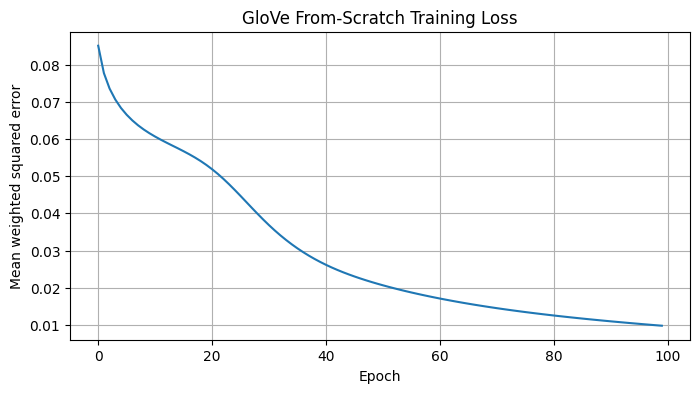
\includegraphics[width=0.82\textwidth,height=0.42\textheight,keepaspectratio]{figs/e6_12_0.png}\caption{GloVe From-Scratch Training Loss}\end{figure}
\Needspace{14\baselineskip}\paragraph{Output 6: custom\_similar\_words = glove\_model.most\_similar(}\mbox{}\\[-1ex]
\begin{Verbatim}[commandchars=\\\{\},breaklines=true,breakanywhere=true,fontsize=\scriptsize,frame=leftline,framesep=2mm,rulecolor=\color{gray}]
Words most similar to 'king' (custom GloVe):
the             0.9740
rules           0.9575
is              0.9378
queen           0.9206
prince          0.9057
princess        0.8858
kingdom         0.8224
books           0.6059
laboratory      0.5980
heat            0.5890
\end{Verbatim}
\Needspace{14\baselineskip}\paragraph{Output 7: try:}\mbox{}\\[-1ex]
\begin{Verbatim}[commandchars=\\\{\},breaklines=true,breakanywhere=true,fontsize=\scriptsize,frame=leftline,framesep=2mm,rulecolor=\color{gray}]
Loading pretrained GloVe vectors. The first run may download the model...
[==================================================] 100.0% 128.1/128.1MB downloaded

Words most similar to 'king' (pretrained GloVe):
prince          0.7682
queen           0.7508
son             0.7021
brother         0.6986
monarch         0.6978
throne          0.6920
kingdom         0.6811
father          0.6802
emperor         0.6713
ii              0.6676
\end{Verbatim}
\Needspace{14\baselineskip}\paragraph{Output 8: comparison\_rows = [}\mbox{}\\[-1ex]
\begin{Verbatim}[commandchars=\\\{\},breaklines=true,breakanywhere=true,fontsize=\scriptsize,frame=leftline,framesep=2mm,rulecolor=\color{gray}]
                              Model  \textbackslash{}
0        Custom GloVe (this corpus)
1  Pretrained GloVe (Wiki-Gigaword)

                                       Similar words
0  the, rules, is, queen, prince, princess, kingd...
1  prince, queen, son, brother, monarch, throne, ...
\end{Verbatim}
\Needspace{14\baselineskip}\paragraph{Output 9: lm\_sentences = [}\mbox{}\\[-1ex]
\begin{Verbatim}[commandchars=\\\{\},breaklines=true,breakanywhere=true,fontsize=\scriptsize,frame=leftline,framesep=2mm,rulecolor=\color{gray}]
['natural', 'language', 'processing', 'is', 'a', 'branch', 'of', 'artificial', 'intelligence']
['natural', 'language', 'processing', 'enables', 'computers', 'to', 'understand', 'human', 'language']
['machine', 'learning', 'is', 'a', 'branch', 'of', 'artificial', 'intelligence']
['deep', 'learning', 'is', 'a', 'part', 'of', 'machine', 'learning']
['language', 'models', 'learn', 'patterns', 'from', 'text', 'data']
['a', 'language', 'model', 'predicts', 'the', 'next', 'word', 'in', 'a', 'sentence']
['natural', 'language', 'processing', 'uses', 'language', 'models']
['artificial', 'intelligence', 'includes', 'machine', 'learning', 'and', 'deep', 'learning']
\end{Verbatim}
\Needspace{14\baselineskip}\paragraph{Output 10: class NGramLanguageModel:}\mbox{}\\[-1ex]
\begin{Verbatim}[commandchars=\\\{\},breaklines=true,breakanywhere=true,fontsize=\scriptsize,frame=leftline,framesep=2mm,rulecolor=\color{gray}]
Bigram count examples:
('<s>', 'natural') : 3
('natural', 'language') : 3
('language', 'processing') : 3
('is', 'a') : 3
('artificial', 'intelligence') : 3
('machine', 'learning') : 3
('a', 'branch') : 2
('branch', 'of') : 2
('of', 'artificial') : 2
('intelligence', '</s>') : 2

Trigram count examples:
('<s>', '<s>', 'natural') : 3
('<s>', 'natural', 'language') : 3
('natural', 'language', 'processing') : 3
('is', 'a', 'branch') : 2
('a', 'branch', 'of') : 2
('branch', 'of', 'artificial') : 2
('of', 'artificial', 'intelligence') : 2
('artificial', 'intelligence', '</s>') : 2
('learning', 'is', 'a') : 2
('language', 'processing', 'is') : 1
\end{Verbatim}
\Needspace{14\baselineskip}\paragraph{Output 11: test\_contexts = [}\mbox{}\\[-1ex]
\begin{Verbatim}[commandchars=\\\{\},breaklines=true,breakanywhere=true,fontsize=\scriptsize,frame=leftline,framesep=2mm,rulecolor=\color{gray}]
Context: 'natural language'
Bigram predictions:
  processing      P=0.0930
  models          P=0.0698
  </s>            P=0.0465
  model           P=0.0465
  <unk>           P=0.0233
Trigram predictions:
  processing      P=0.1026
  </s>            P=0.0256
  <unk>           P=0.0256
  a               P=0.0256
  and             P=0.0256

Context: 'machine learning'
Bigram predictions:
  </s>            P=0.0732
  is              P=0.0732
  and             P=0.0488
  <unk>           P=0.0244
  a               P=0.0244
Trigram predictions:
  </s>            P=0.0513
  and             P=0.0513
  is              P=0.0513
  <unk>           P=0.0256
  a               P=0.0256

Context: 'artificial intelligence'
Bigram predictions:
  </s>            P=0.0769
  includes        P=0.0513
  <unk>           P=0.0256
  a               P=0.0256
  and             P=0.0256
Trigram predictions:
  </s>            P=0.0769
  includes        P=0.0513
  <unk>           P=0.0256
  a               P=0.0256
  and             P=0.0256

Context: 'a language model'
Bigram predictions:
  predicts        P=0.0541
... [output truncated for length]
\end{Verbatim}
\Needspace{14\baselineskip}\paragraph{Output 12: context\_to\_test = "machine learning"}\mbox{}\\[-1ex]
\begin{Verbatim}[commandchars=\\\{\},breaklines=true,breakanywhere=true,fontsize=\scriptsize,frame=leftline,framesep=2mm,rulecolor=\color{gray}]
Context: machine learning

Bigram model:
1. </s>  (probability=0.0732)
2. is  (probability=0.0732)
3. and  (probability=0.0488)
4. <unk>  (probability=0.0244)
5. a  (probability=0.0244)

Trigram model:
1. </s>  (probability=0.0513)
2. and  (probability=0.0513)
3. is  (probability=0.0513)
4. <unk>  (probability=0.0256)
5. a  (probability=0.0256)
\end{Verbatim}
\Needspace{14\baselineskip}\paragraph{Output 13: context = "machine learning"}\mbox{}\\[-1ex]
\begin{Verbatim}[commandchars=\\\{\},breaklines=true,breakanywhere=true,fontsize=\scriptsize,frame=leftline,framesep=2mm,rulecolor=\color{gray}]
P('is' | 'machine learning')
Bigram : 0.073171
Trigram: 0.051282
\end{Verbatim}
\textbf{Observations.}

\begin{itemize}
\tightlist
\item
  Training loss for the from-scratch GloVe model fell from 0.0851 in epoch 1 to 0.0098 in epoch 100.
\item
  On the tiny corpus, the nearest words to \emph{king} include frequent function words (\emph{the}, \emph{rules}, \emph{is}) and then \emph{queen} (0.921), \emph{prince} (0.906), \emph{princess} (0.886) and \emph{kingdom} (0.822). The royalty words are present but share the list with frequent words because the corpus is so small.
\item
  The pretrained Gensim vectors, trained on a very large corpus, return semantically clean neighbours led by \emph{prince} (0.768) and \emph{queen}.
\item
  For the context \emph{natural language}, the bigram model ranks \emph{processing} highest (\(P=0.0930\)). For \emph{machine learning}, \(P(\text{is})=0.0732\) for the bigram and \(0.0513\) for the trigram model, since the trigram model spreads probability over more sparse contexts and benefits less from smoothing on such a small corpus.
\end{itemize}


\section{Conclusion}
GloVe captures related words (royalty terms) even from a 24-sentence corpus, but the quality of the neighbours depends strongly on corpus size, which is why the pretrained vectors are cleaner. The N-gram models predict plausible next words, and the comparison shows the sparsity problem that grows with the order of the model.


\chapter{Experiment 7: Text Classification Using Deep Learning Models (IMDB Sentiment)}
\section{Abstract}
This experiment performs binary sentiment classification on the IMDB movie-review dataset with four models: Logistic Regression on TF-IDF features, an LSTM, a Transformer encoder built from scratch and a fine-tuned pretrained BERT. The models are compared on the same held-out test set using accuracy, precision, recall, F1-score and confusion matrices.


\section{Aim}
To implement and compare classical, recurrent, transformer and pretrained-transformer models for sentiment classification.


\section{Objectives}
\begin{itemize}
\item Implement sentiment classification with Logistic Regression, an LSTM, a vanilla Transformer encoder and fine-tuned BERT.
\item Evaluate all models with precision, recall and F1-score on the same test set.
\item Analyse errors through confusion matrices and test the models on custom reviews.
\end{itemize}

\section{Description and Theoretical Background}
Logistic Regression over TF-IDF vectors is a bag-of-words baseline that ignores word order. An \textbf{LSTM} reads the token sequence and keeps a hidden state. A \textbf{Transformer encoder} uses multi-head self-attention, positional embeddings, residual connections and layer normalisation; trained from scratch it must learn language from the task data alone. \textbf{BERT} is a bidirectional Transformer pretrained on large corpora and fine-tuned with a classification head, which transfers general language knowledge to the task. Precision, recall and F1 are computed with the positive class as the positive label.


\section{Data Understanding}
The IMDB Dataset of 50K Movie Reviews (\texttt{IMDB\ Dataset.csv}, columns \texttt{review} and \texttt{sentiment}). After removing missing rows and duplicate reviews, \textbf{49,582} reviews remained. A stratified split gave \textbf{35,698} training, \textbf{3,967} validation and \textbf{9,917} test reviews.


\section{Data Preprocessing}
Labels are encoded as 0 (negative) and 1 (positive). Logistic Regression uses TF-IDF with up to 50,000 unigram and bigram features and English stopword removal. The LSTM and Transformer use a vocabulary built from the neural training subset only (maximum 30,000 words, with padding and unknown tokens) and a maximum sequence length of 200. The neural models were trained on a 10,000-review subset to limit training time; BERT used its own tokenizer.


\section{Description of the Implemented Code}
Shared utilities compute metrics and run the training and prediction loops with the Adam optimiser, cross-entropy loss and validation-F1 checkpoint selection. \texttt{LSTMClassifier} and \texttt{TransformerClassifier} are PyTorch modules; BERT is \texttt{bert-base-uncased} loaded with \texttt{AutoModelForSequenceClassification} and fine-tuned for two epochs. All models are scored on the identical test split and compared in a results table, bar chart and four confusion matrices.


\section{Implemented Code}
\Needspace{8\baselineskip}\paragraph{Listing 1: accuracy\_score, precision\_score, recall\_score, f1\_score,}\mbox{}\\[-1ex]
\begin{Verbatim}[commandchars=\\\{\},breaklines=true,breakanywhere=true,fontsize=\scriptsize,frame=leftline,framesep=2mm,rulecolor=\color{gray}]
import os
import re
import copy
import random
import warnings
import numpy as np
import pandas as pd
import matplotlib.pyplot as plt
import seaborn as sns

from collections import Counter
from sklearn.model_selection import train_test_split
from sklearn.feature_extraction.text import TfidfVectorizer
from sklearn.linear_model import LogisticRegression
from sklearn.metrics import (
    accuracy_score, precision_score, recall_score, f1_score,
    classification_report, confusion_matrix
)

import torch
import torch.nn as nn
from torch.utils.data import Dataset, DataLoader
from tqdm.auto import tqdm

warnings.filterwarnings("ignore")

SEED = 42
random.seed(SEED)
np.random.seed(SEED)
torch.manual_seed(SEED)
if torch.cuda.is_available():
    torch.cuda.manual_seed_all(SEED)

DEVICE = torch.device("cuda" if torch.cuda.is_available() else "cpu")
print("PyTorch version:", torch.__version__)
print("Execution device:", DEVICE)
\end{Verbatim}
\Needspace{8\baselineskip}\paragraph{Listing 2: Colab upload fallback. On a local Jupyter installation, place the CSV}\mbox{}\\[-1ex]
\begin{Verbatim}[commandchars=\\\{\},breaklines=true,breakanywhere=true,fontsize=\scriptsize,frame=leftline,framesep=2mm,rulecolor=\color{gray}]
from pathlib import Path

DATA_PATH = Path("IMDB Dataset.csv")

if not DATA_PATH.exists():
    # Colab upload fallback. On a local Jupyter installation, place the CSV
    # in the same directory as this notebook and rerun this cell.
    try:
        from google.colab import files
        print("Upload the IMDB Dataset.csv file.")
        uploaded = files.upload()
        csv_names = [name for name in uploaded if name.lower().endswith(".csv")]
        if csv_names:
            DATA_PATH = Path(csv_names[0])
    except ImportError:
        print("Google Colab upload is unavailable. Place 'IMDB Dataset.csv' beside this notebook.")

if not DATA_PATH.exists():
    raise FileNotFoundError(
        "Dataset not found. Download 'IMDB Dataset.csv' from the Kaggle link in the experiment sheet "
        "and place it in the notebook directory."
    )

df = pd.read_csv(DATA_PATH)
print("Dataset shape:", df.shape)
display(df.head())
print("\textbackslash{}nColumns:", df.columns.tolist())
\end{Verbatim}
\Needspace{8\baselineskip}\paragraph{Listing 3: required\_columns = \{"review", "sentiment"\}}\mbox{}\\[-1ex]
\begin{Verbatim}[commandchars=\\\{\},breaklines=true,breakanywhere=true,fontsize=\scriptsize,frame=leftline,framesep=2mm,rulecolor=\color{gray}]
required_columns = \textbraceleft{}"review", "sentiment"\textbraceright{}
if not required_columns.issubset(set(df.columns)):
    raise ValueError(
        f"Expected columns \textbraceleft{}required_columns\textbraceright{}, but found \textbraceleft{}set(df.columns)\textbraceright{}"
    )

df = df[["review", "sentiment"]].dropna().drop_duplicates().copy()
df["review"] = df["review"].astype(str)
df["sentiment"] = df["sentiment"].astype(str).str.strip().str.lower()

label_map = \textbraceleft{}"negative": 0, "positive": 1\textbraceright{}
unexpected = set(df["sentiment"].unique()) - set(label_map)
if unexpected:
    raise ValueError(f"Unexpected sentiment labels: \textbraceleft{}unexpected\textbraceright{}")

df["label"] = df["sentiment"].map(label_map).astype(int)
df = df.reset_index(drop=True)

print("Cleaned dataset shape:", df.shape)
print("\textbackslash{}nClass distribution:")
display(df["sentiment"].value_counts().to_frame("count"))
print("\textbackslash{}nMissing values:")
display(df.isnull().sum().to_frame("missing values"))
\end{Verbatim}
\Needspace{8\baselineskip}\paragraph{Listing 4: plt.figure(figsize=(6, 4))}\mbox{}\\[-1ex]
\begin{Verbatim}[commandchars=\\\{\},breaklines=true,breakanywhere=true,fontsize=\scriptsize,frame=leftline,framesep=2mm,rulecolor=\color{gray}]
plt.figure(figsize=(6, 4))
sns.countplot(data=df, x="sentiment")
plt.title("Distribution of IMDB Sentiment Labels")
plt.xlabel("Sentiment")
plt.ylabel("Number of reviews")
plt.show()
\end{Verbatim}
\Needspace{8\baselineskip}\paragraph{Listing 5: X = df["review"].values}\mbox{}\\[-1ex]
\begin{Verbatim}[commandchars=\\\{\},breaklines=true,breakanywhere=true,fontsize=\scriptsize,frame=leftline,framesep=2mm,rulecolor=\color{gray}]
X = df["review"].values
y = df["label"].values

X_train_full, X_test, y_train_full, y_test = train_test_split(
    X, y, test_size=0.20, random_state=SEED, stratify=y
)
X_train, X_val, y_train, y_val = train_test_split(
    X_train_full, y_train_full, test_size=0.10,
    random_state=SEED, stratify=y_train_full
)

print(f"Training samples:   \textbraceleft{}len(X_train):,\textbraceright{}")
print(f"Validation samples: \textbraceleft{}len(X_val):,\textbraceright{}")
print(f"Testing samples:    \textbraceleft{}len(X_test):,\textbraceright{}")
\end{Verbatim}
\Needspace{8\baselineskip}\paragraph{Listing 6: NEURAL\_TRAIN\_LIMIT = 10000   \# Set to None to use the complete trainin}\mbox{}\\[-1ex]
\begin{Verbatim}[commandchars=\\\{\},breaklines=true,breakanywhere=true,fontsize=\scriptsize,frame=leftline,framesep=2mm,rulecolor=\color{gray}]
NEURAL_TRAIN_LIMIT = 10000   # Set to None to use the complete training split
MAX_VOCAB_SIZE = 30000
MAX_SEQ_LEN = 200
BATCH_SIZE = 64
NEURAL_EPOCHS = 3
LEARNING_RATE = 1e-3

def stratified_cap(texts, labels, limit, seed=SEED):
    if limit is None or limit >= len(texts):
        return np.asarray(texts), np.asarray(labels)
    x_keep, _, y_keep, _ = train_test_split(
        texts, labels, train_size=limit, random_state=seed, stratify=labels
    )
    return np.asarray(x_keep), np.asarray(y_keep)

X_nn_train, y_nn_train = stratified_cap(
    X_train, y_train, NEURAL_TRAIN_LIMIT
)
print("Neural training subset:", len(X_nn_train))
\end{Verbatim}
\Needspace{8\baselineskip}\paragraph{Listing 7: tfidf = TfidfVectorizer(}\mbox{}\\[-1ex]
\begin{Verbatim}[commandchars=\\\{\},breaklines=true,breakanywhere=true,fontsize=\scriptsize,frame=leftline,framesep=2mm,rulecolor=\color{gray}]
tfidf = TfidfVectorizer(
    max_features=50000,
    ngram_range=(1, 2),
    stop_words="english",
    min_df=2,
    max_df=0.95,
    sublinear_tf=True
)

X_train_tfidf = tfidf.fit_transform(X_train)
X_val_tfidf = tfidf.transform(X_val)
X_test_tfidf = tfidf.transform(X_test)

print("TF-IDF training matrix:", X_train_tfidf.shape)
\end{Verbatim}
\Needspace{8\baselineskip}\paragraph{Listing 8: logreg = LogisticRegression(}\mbox{}\\[-1ex]
\begin{Verbatim}[commandchars=\\\{\},breaklines=true,breakanywhere=true,fontsize=\scriptsize,frame=leftline,framesep=2mm,rulecolor=\color{gray}]
logreg = LogisticRegression(
    max_iter=1000,
    C=2.0,
    solver="liblinear",
    random_state=SEED
)
logreg.fit(X_train_tfidf, y_train)

lr_val_pred = logreg.predict(X_val_tfidf)
print(classification_report(
    y_val, lr_val_pred, target_names=["negative", "positive"]
))
\end{Verbatim}
\Needspace{8\baselineskip}\paragraph{Listing 9: PAD\_TOKEN = "<pad>"}\mbox{}\\[-1ex]
\begin{Verbatim}[commandchars=\\\{\},breaklines=true,breakanywhere=true,fontsize=\scriptsize,frame=leftline,framesep=2mm,rulecolor=\color{gray}]
PAD_TOKEN = "<pad>"
UNK_TOKEN = "<unk>"

def basic_tokenize(text):
    return re.findall(r"[a-z0-9']+", str(text).lower())

token_counts = Counter()
for review in tqdm(X_nn_train, desc="Building vocabulary"):
    token_counts.update(basic_tokenize(review))

vocab = \textbraceleft{}PAD_TOKEN: 0, UNK_TOKEN: 1\textbraceright{}
for token, count in token_counts.most_common(MAX_VOCAB_SIZE - 2):
    vocab[token] = len(vocab)

print("Vocabulary size:", len(vocab))

def encode_review(text, max_len=MAX_SEQ_LEN):
    ids = [vocab.get(token, vocab[UNK_TOKEN]) for token in basic_tokenize(text)]
    ids = ids[:max_len]
    if not ids:
        ids = [vocab[UNK_TOKEN]]
    return ids

class ReviewDataset(Dataset):
    def __init__(self, texts, labels, max_len=MAX_SEQ_LEN):
        self.texts = list(texts)
        self.labels = np.asarray(labels, dtype=np.int64)
        self.max_len = max_len

    def __len__(self):
        return len(self.texts)

    def __getitem__(self, index):
        ids = encode_review(self.texts[index], self.max_len)
        return torch.tensor(ids, dtype=torch.long), torch.tensor(self.labels[index], dtype=torch.long)

def collate_reviews(batch):
    sequences, labels = zip(*batch)
    lengths = torch.tensor([len(seq) for seq in sequences], dtype=torch.long)
    padded = nn.utils.rnn.pad_sequence(
        sequences, batch_first=True, padding_value=vocab[PAD_TOKEN]
    )
    return padded, lengths, torch.stack(labels)

train_dataset = ReviewDataset(X_nn_train, y_nn_train)
val_dataset = ReviewDataset(X_val, y_val)
test_dataset = ReviewDataset(X_test, y_test)

train_loader = DataLoader(
    train_dataset, batch_size=BATCH_SIZE, shuffle=True, collate_fn=collate_reviews
)
val_loader = DataLoader(
    val_dataset, batch_size=BATCH_SIZE, shuffle=False, collate_fn=collate_reviews
)
test_loader = DataLoader(
    test_dataset, batch_size=BATCH_SIZE, shuffle=False, collate_fn=collate_reviews
)

print("Neural data loaders ready.")
\end{Verbatim}
\Needspace{8\baselineskip}\paragraph{Listing 10: def calculate\_metrics(y\_true, y\_pred):}\mbox{}\\[-1ex]
\begin{Verbatim}[commandchars=\\\{\},breaklines=true,breakanywhere=true,fontsize=\scriptsize,frame=leftline,framesep=2mm,rulecolor=\color{gray}]
def calculate_metrics(y_true, y_pred):
    return \textbraceleft{}
        "Accuracy": accuracy_score(y_true, y_pred),
        "Precision": precision_score(y_true, y_pred, zero_division=0),
        "Recall": recall_score(y_true, y_pred, zero_division=0),
        "F1-score": f1_score(y_true, y_pred, zero_division=0)
    \textbraceright{}

def train_torch_model(model, train_loader, val_loader, epochs=NEURAL_EPOCHS, lr=LEARNING_RATE):
    model = model.to(DEVICE)
    optimizer = torch.optim.Adam(model.parameters(), lr=lr)
    criterion = nn.CrossEntropyLoss()
    best_f1 = -1
    best_state = copy.deepcopy(model.state_dict())
    history = []

    for epoch in range(epochs):
        model.train()
        running_loss = 0.0

        for input_ids, lengths, labels in tqdm(train_loader, desc=f"Epoch \textbraceleft{}epoch+1\textbraceright{}/\textbraceleft{}epochs\textbraceright{}"):
            input_ids = input_ids.to(DEVICE)
            lengths = lengths.to(DEVICE)
            labels = labels.to(DEVICE)

            optimizer.zero_grad()
            logits = model(input_ids, lengths)
            loss = criterion(logits, labels)
            loss.backward()
            nn.utils.clip_grad_norm_(model.parameters(), max_norm=1.0)
            optimizer.step()
            running_loss += loss.item()

        val_true, val_pred = predict_torch_model(model, val_loader)
        metrics = calculate_metrics(val_true, val_pred)
        avg_loss = running_loss / max(len(train_loader), 1)
        history.append(\textbraceleft{}"epoch": epoch + 1, "loss": avg_loss, **metrics\textbraceright{})

        print(
            f"Epoch \textbraceleft{}epoch+1\textbraceright{}: loss=\textbraceleft{}avg_loss:.4f\textbraceright{}, "
            f"val_precision=\textbraceleft{}metrics['Precision']:.4f\textbraceright{}, "
            f"val_recall=\textbraceleft{}metrics['Recall']:.4f\textbraceright{}, "
            f"val_f1=\textbraceleft{}metrics['F1-score']:.4f\textbraceright{}"
        )

        if metrics["F1-score"] > best_f1:
            best_f1 = metrics["F1-score"]
            best_state = copy.deepcopy(model.state_dict())

    model.load_state_dict(best_state)
    return model, pd.DataFrame(history)

@torch.no_grad()
def predict_torch_model(model, loader):
    model.eval()
    all_true, all_pred = [], []
    for input_ids, lengths, labels in loader:
        input_ids = input_ids.to(DEVICE)
        lengths = lengths.to(DEVICE)
        logits = model(input_ids, lengths)
        predictions = torch.argmax(logits, dim=1).cpu().numpy()
        all_pred.extend(predictions)
        all_true.extend(labels.numpy())
    return np.asarray(all_true), np.asarray(all_pred)

def plot_training_history(history, title):
    plt.figure(figsize=(7, 4))
    plt.plot(history["epoch"], history["loss"], marker="o", label="Training loss")
    plt.xlabel("Epoch")
    plt.ylabel("Loss")
    plt.title(title)
    plt.grid(True)
    plt.legend()
    plt.show()
\end{Verbatim}
\Needspace{8\baselineskip}\paragraph{Listing 11: Concatenate final forward and backward hidden states.}\mbox{}\\[-1ex]
\begin{Verbatim}[commandchars=\\\{\},breaklines=true,breakanywhere=true,fontsize=\scriptsize,frame=leftline,framesep=2mm,rulecolor=\color{gray}]
class LSTMClassifier(nn.Module):
    def __init__(self, vocab_size, embedding_dim=128, hidden_dim=128, num_layers=1, dropout=0.3):
        super().__init__()
        self.embedding = nn.Embedding(vocab_size, embedding_dim, padding_idx=vocab[PAD_TOKEN])
        self.lstm = nn.LSTM(
            embedding_dim, hidden_dim, num_layers=num_layers,
            batch_first=True, bidirectional=True,
            dropout=dropout if num_layers > 1 else 0
        )
        self.dropout = nn.Dropout(dropout)
        self.fc = nn.Linear(hidden_dim * 2, 2)

    def forward(self, input_ids, lengths):
        embedded = self.embedding(input_ids)
        packed = nn.utils.rnn.pack_padded_sequence(
            embedded, lengths.cpu(), batch_first=True, enforce_sorted=False
        )
        _, (hidden, _) = self.lstm(packed)
        # Concatenate final forward and backward hidden states.
        representation = torch.cat((hidden[-2], hidden[-1]), dim=1)
        return self.fc(self.dropout(representation))

lstm_model = LSTMClassifier(len(vocab))
lstm_model, lstm_history = train_torch_model(
    lstm_model, train_loader, val_loader,
    epochs=NEURAL_EPOCHS, lr=LEARNING_RATE
)
plot_training_history(lstm_history, "LSTM Training Loss")
\end{Verbatim}
\Needspace{8\baselineskip}\paragraph{Listing 12: lstm\_y\_true, lstm\_y\_pred = predict\_torch\_model(lstm\_model, test\_loader}\mbox{}\\[-1ex]
\begin{Verbatim}[commandchars=\\\{\},breaklines=true,breakanywhere=true,fontsize=\scriptsize,frame=leftline,framesep=2mm,rulecolor=\color{gray}]
lstm_y_true, lstm_y_pred = predict_torch_model(lstm_model, test_loader)
lstm_metrics = calculate_metrics(lstm_y_true, lstm_y_pred)
print("LSTM Test Metrics:", lstm_metrics)
print(classification_report(
    lstm_y_true, lstm_y_pred, target_names=["negative", "positive"]
))
\end{Verbatim}
\Needspace{8\baselineskip}\paragraph{Listing 13: class TransformerClassifier(nn.Module):}\mbox{}\\[-1ex]
\begin{Verbatim}[commandchars=\\\{\},breaklines=true,breakanywhere=true,fontsize=\scriptsize,frame=leftline,framesep=2mm,rulecolor=\color{gray}]
class TransformerClassifier(nn.Module):
    def __init__(
        self, vocab_size, max_len=MAX_SEQ_LEN, embedding_dim=128,
        num_heads=4, num_layers=2, ff_dim=256, dropout=0.2
    ):
        super().__init__()
        self.token_embedding = nn.Embedding(
            vocab_size, embedding_dim, padding_idx=vocab[PAD_TOKEN]
        )
        self.position_embedding = nn.Embedding(max_len, embedding_dim)

        encoder_layer = nn.TransformerEncoderLayer(
            d_model=embedding_dim,
            nhead=num_heads,
            dim_feedforward=ff_dim,
            dropout=dropout,
            batch_first=True,
            activation="gelu"
        )
        self.encoder = nn.TransformerEncoder(encoder_layer, num_layers=num_layers)
        self.dropout = nn.Dropout(dropout)
        self.classifier = nn.Linear(embedding_dim, 2)
        self.max_len = max_len

    def forward(self, input_ids, lengths):
        batch_size, seq_len = input_ids.shape
        positions = torch.arange(seq_len, device=input_ids.device).unsqueeze(0).expand(batch_size, -1)
        x = self.token_embedding(input_ids) + self.position_embedding(positions)

        padding_mask = input_ids.eq(vocab[PAD_TOKEN])
        encoded = self.encoder(x, src_key_padding_mask=padding_mask)

        valid_mask = (~padding_mask).unsqueeze(-1).float()
        pooled = (encoded * valid_mask).sum(dim=1) / valid_mask.sum(dim=1).clamp(min=1.0)
        return self.classifier(self.dropout(pooled))

transformer_model = TransformerClassifier(len(vocab))
transformer_model, transformer_history = train_torch_model(
    transformer_model, train_loader, val_loader,
    epochs=NEURAL_EPOCHS, lr=LEARNING_RATE
)
plot_training_history(transformer_history, "Vanilla Transformer Training Loss")
\end{Verbatim}
\Needspace{8\baselineskip}\paragraph{Listing 14: transformer\_y\_true, transformer\_y\_pred = predict\_torch\_model(}\mbox{}\\[-1ex]
\begin{Verbatim}[commandchars=\\\{\},breaklines=true,breakanywhere=true,fontsize=\scriptsize,frame=leftline,framesep=2mm,rulecolor=\color{gray}]
transformer_y_true, transformer_y_pred = predict_torch_model(
    transformer_model, test_loader
)
transformer_metrics = calculate_metrics(transformer_y_true, transformer_y_pred)
print("Vanilla Transformer Test Metrics:", transformer_metrics)
print(classification_report(
    transformer_y_true, transformer_y_pred,
    target_names=["negative", "positive"]
))
\end{Verbatim}
\Needspace{8\baselineskip}\paragraph{Listing 15: BERT\_MODEL\_NAME = "bert-base-uncased"}\mbox{}\\[-1ex]
\begin{Verbatim}[commandchars=\\\{\},breaklines=true,breakanywhere=true,fontsize=\scriptsize,frame=leftline,framesep=2mm,rulecolor=\color{gray}]
from transformers import AutoTokenizer, AutoModelForSequenceClassification
from torch.utils.data import Dataset, DataLoader

BERT_MODEL_NAME = "bert-base-uncased"
BERT_MAX_LEN = 256
BERT_BATCH_SIZE = 8 if DEVICE.type == "cpu" else 16
BERT_EPOCHS = 2
BERT_TRAIN_LIMIT = 5000  # Set to None to use all training examples

bert_tokenizer = AutoTokenizer.from_pretrained(BERT_MODEL_NAME)
bert_model = AutoModelForSequenceClassification.from_pretrained(
    BERT_MODEL_NAME, num_labels=2
).to(DEVICE)

X_bert_train, y_bert_train = stratified_cap(
    X_train, y_train, BERT_TRAIN_LIMIT
)
print("BERT training samples:", len(X_bert_train))
print("BERT device:", DEVICE)
\end{Verbatim}
\Needspace{8\baselineskip}\paragraph{Listing 16: class BertReviewDataset(Dataset):}\mbox{}\\[-1ex]
\begin{Verbatim}[commandchars=\\\{\},breaklines=true,breakanywhere=true,fontsize=\scriptsize,frame=leftline,framesep=2mm,rulecolor=\color{gray}]
class BertReviewDataset(Dataset):
    def __init__(self, texts, labels, tokenizer, max_len=BERT_MAX_LEN):
        self.encodings = tokenizer(
            list(texts),
            truncation=True,
            padding="max_length",
            max_length=max_len,
            return_tensors="pt"
        )
        self.labels = torch.tensor(np.asarray(labels), dtype=torch.long)

    def __len__(self):
        return len(self.labels)

    def __getitem__(self, idx):
        item = \textbraceleft{}key: value[idx] for key, value in self.encodings.items()\textbraceright{}
        item["labels"] = self.labels[idx]
        return item

bert_train_dataset = BertReviewDataset(
    X_bert_train, y_bert_train, bert_tokenizer
)
bert_val_dataset = BertReviewDataset(X_val, y_val, bert_tokenizer)
bert_test_dataset = BertReviewDataset(X_test, y_test, bert_tokenizer)

bert_train_loader = DataLoader(
    bert_train_dataset, batch_size=BERT_BATCH_SIZE, shuffle=True
)
bert_val_loader = DataLoader(
    bert_val_dataset, batch_size=BERT_BATCH_SIZE
)
bert_test_loader = DataLoader(
    bert_test_dataset, batch_size=BERT_BATCH_SIZE
)

print("BERT data loaders ready.")
\end{Verbatim}
\Needspace{8\baselineskip}\paragraph{Listing 17: def evaluate\_bert(model, loader):}\mbox{}\\[-1ex]
\begin{Verbatim}[commandchars=\\\{\},breaklines=true,breakanywhere=true,fontsize=\scriptsize,frame=leftline,framesep=2mm,rulecolor=\color{gray}]
def evaluate_bert(model, loader):
    model.eval()
    y_true, y_pred = [], []
    with torch.no_grad():
        for batch in loader:
            batch = \textbraceleft{}k: v.to(DEVICE) for k, v in batch.items()\textbraceright{}
            labels = batch.pop("labels")
            outputs = model(**batch)
            preds = torch.argmax(outputs.logits, dim=1)
            y_true.extend(labels.cpu().numpy())
            y_pred.extend(preds.cpu().numpy())
    return np.asarray(y_true), np.asarray(y_pred)

bert_optimizer = torch.optim.AdamW(bert_model.parameters(), lr=2e-5)
bert_history = []
best_bert_f1 = -1
best_bert_state = copy.deepcopy(bert_model.state_dict())
scaler = torch.cuda.amp.GradScaler(enabled=(DEVICE.type == "cuda"))

for epoch in range(BERT_EPOCHS):
    bert_model.train()
    total_loss = 0.0

    for batch in tqdm(bert_train_loader, desc=f"BERT Epoch \textbraceleft{}epoch+1\textbraceright{}/\textbraceleft{}BERT_EPOCHS\textbraceright{}"):
        batch = \textbraceleft{}k: v.to(DEVICE) for k, v in batch.items()\textbraceright{}
        bert_optimizer.zero_grad()

        with torch.cuda.amp.autocast(enabled=(DEVICE.type == "cuda")):
            outputs = bert_model(**batch)
            loss = outputs.loss

        scaler.scale(loss).backward()
        scaler.unscale_(bert_optimizer)
        nn.utils.clip_grad_norm_(bert_model.parameters(), 1.0)
        scaler.step(bert_optimizer)
        scaler.update()
        total_loss += loss.item()

    val_true, val_pred = evaluate_bert(bert_model, bert_val_loader)
    val_metrics = calculate_metrics(val_true, val_pred)
    avg_loss = total_loss / max(len(bert_train_loader), 1)
    bert_history.append(\textbraceleft{}"epoch": epoch + 1, "loss": avg_loss, **val_metrics\textbraceright{})

    print(
        f"Epoch \textbraceleft{}epoch+1\textbraceright{}: loss=\textbraceleft{}avg_loss:.4f\textbraceright{}, "
        f"val_precision=\textbraceleft{}val_metrics['Precision']:.4f\textbraceright{}, "
        f"val_recall=\textbraceleft{}val_metrics['Recall']:.4f\textbraceright{}, "
        f"val_f1=\textbraceleft{}val_metrics['F1-score']:.4f\textbraceright{}"
    )

    if val_metrics["F1-score"] > best_bert_f1:
        best_bert_f1 = val_metrics["F1-score"]
        best_bert_state = copy.deepcopy(bert_model.state_dict())

bert_model.load_state_dict(best_bert_state)
bert_history = pd.DataFrame(bert_history)

plt.figure(figsize=(7, 4))
plt.plot(bert_history["epoch"], bert_history["loss"], marker="o")
plt.xlabel("Epoch")
plt.ylabel("Training loss")
plt.title("BERT Fine-tuning Loss")
plt.grid(True)
plt.show()
\end{Verbatim}
\Needspace{8\baselineskip}\paragraph{Listing 18: bert\_y\_true, bert\_y\_pred = evaluate\_bert(bert\_model, bert\_test\_loader)}\mbox{}\\[-1ex]
\begin{Verbatim}[commandchars=\\\{\},breaklines=true,breakanywhere=true,fontsize=\scriptsize,frame=leftline,framesep=2mm,rulecolor=\color{gray}]
bert_y_true, bert_y_pred = evaluate_bert(bert_model, bert_test_loader)
bert_metrics = calculate_metrics(bert_y_true, bert_y_pred)

print("BERT Test Metrics:", bert_metrics)
print(classification_report(
    bert_y_true, bert_y_pred, target_names=["negative", "positive"]
))
\end{Verbatim}
\Needspace{8\baselineskip}\paragraph{Listing 19: Logistic Regression test predictions}\mbox{}\\[-1ex]
\begin{Verbatim}[commandchars=\\\{\},breaklines=true,breakanywhere=true,fontsize=\scriptsize,frame=leftline,framesep=2mm,rulecolor=\color{gray}]
# Logistic Regression test predictions
lr_y_pred = logreg.predict(X_test_tfidf)
lr_metrics = calculate_metrics(y_test, lr_y_pred)

results = \textbraceleft{}
    "Logistic Regression": lr_metrics,
    "LSTM": lstm_metrics,
    "Vanilla Transformer": transformer_metrics,
    "BERT (bert-base-uncased)": bert_metrics
\textbraceright{}

results_df = pd.DataFrame(results).T
display(results_df.round(4))
\end{Verbatim}
\Needspace{8\baselineskip}\paragraph{Listing 20: metrics\_to\_plot = ["Precision", "Recall", "F1-score"]}\mbox{}\\[-1ex]
\begin{Verbatim}[commandchars=\\\{\},breaklines=true,breakanywhere=true,fontsize=\scriptsize,frame=leftline,framesep=2mm,rulecolor=\color{gray}]
metrics_to_plot = ["Precision", "Recall", "F1-score"]
results_df[metrics_to_plot].plot(
    kind="bar", figsize=(11, 5), ylim=(0, 1),
    title="Model Comparison on IMDB Test Set"
)
plt.ylabel("Score")
plt.xlabel("Model")
plt.xticks(rotation=20, ha="right")
plt.grid(axis="y", alpha=0.3)
plt.legend(loc="lower right")
plt.tight_layout()
plt.show()
\end{Verbatim}
\Needspace{8\baselineskip}\paragraph{Listing 21: all\_predictions = \{}\mbox{}\\[-1ex]
\begin{Verbatim}[commandchars=\\\{\},breaklines=true,breakanywhere=true,fontsize=\scriptsize,frame=leftline,framesep=2mm,rulecolor=\color{gray}]
all_predictions = \textbraceleft{}
    "Logistic Regression": (y_test, lr_y_pred),
    "LSTM": (lstm_y_true, lstm_y_pred),
    "Vanilla Transformer": (transformer_y_true, transformer_y_pred),
    "BERT": (bert_y_true, bert_y_pred)
\textbraceright{}

fig, axes = plt.subplots(2, 2, figsize=(12, 10))
for ax, (model_name, (true_labels, predicted_labels)) in zip(
    axes.flatten(), all_predictions.items()
):
    cm = confusion_matrix(true_labels, predicted_labels, labels=[0, 1])
    sns.heatmap(
        cm, annot=True, fmt="d", cmap="Blues", cbar=False, ax=ax,
        xticklabels=["negative", "positive"],
        yticklabels=["negative", "positive"]
    )
    ax.set_title(model_name)
    ax.set_xlabel("Predicted label")
    ax.set_ylabel("Actual label")

plt.tight_layout()
plt.show()
\end{Verbatim}
\Needspace{8\baselineskip}\paragraph{Listing 22: for model\_name, (true\_labels, predicted\_labels) in all\_predictions.ite}\mbox{}\\[-1ex]
\begin{Verbatim}[commandchars=\\\{\},breaklines=true,breakanywhere=true,fontsize=\scriptsize,frame=leftline,framesep=2mm,rulecolor=\color{gray}]
for model_name, (true_labels, predicted_labels) in all_predictions.items():
    print("=" * 70)
    print(model_name)
    print(classification_report(
        true_labels, predicted_labels,
        labels=[0, 1], target_names=["negative", "positive"],
        zero_division=0
    ))
\end{Verbatim}
\Needspace{8\baselineskip}\paragraph{Listing 23: Logistic Regression}\mbox{}\\[-1ex]
\begin{Verbatim}[commandchars=\\\{\},breaklines=true,breakanywhere=true,fontsize=\scriptsize,frame=leftline,framesep=2mm,rulecolor=\color{gray}]
def predict_custom_review(review_text):
    # Logistic Regression
    lr_vector = tfidf.transform([review_text])
    lr_pred = int(logreg.predict(lr_vector)[0])

    # LSTM
    lstm_ids = encode_review(review_text)
    lstm_input = torch.tensor([lstm_ids], dtype=torch.long).to(DEVICE)
    lstm_lengths = torch.tensor([len(lstm_ids)], dtype=torch.long).to(DEVICE)
    lstm_model.eval()
    with torch.no_grad():
        lstm_pred = int(torch.argmax(lstm_model(lstm_input, lstm_lengths), dim=1).item())

    # Vanilla Transformer
    transformer_model.eval()
    with torch.no_grad():
        transformer_pred = int(torch.argmax(
            transformer_model(lstm_input, lstm_lengths), dim=1
        ).item())

    # BERT
    encoded = bert_tokenizer(
        review_text, return_tensors="pt", truncation=True,
        padding="max_length", max_length=BERT_MAX_LEN
    )
    encoded = \textbraceleft{}k: v.to(DEVICE) for k, v in encoded.items()\textbraceright{}
    bert_model.eval()
    with torch.no_grad():
        bert_pred = int(torch.argmax(bert_model(**encoded).logits, dim=1).item())

    label_names = \textbraceleft{}0: "Negative", 1: "Positive"\textbraceright{}
    return pd.DataFrame(\textbraceleft{}
        "Model": ["Logistic Regression", "LSTM", "Vanilla Transformer", "BERT"],
        "Predicted sentiment": [
            label_names[lr_pred], label_names[lstm_pred],
            label_names[transformer_pred], label_names[bert_pred]
        ]
    \textbraceright{})

sample_review = "The movie was beautifully directed and the performances were excellent."
display(predict_custom_review(sample_review))
\end{Verbatim}

\section{Results and Observations}
\Needspace{14\baselineskip}\paragraph{Output 1: accuracy\_score, precision\_score, recall\_score, f1\_score,}\mbox{}\\[-1ex]
\begin{Verbatim}[commandchars=\\\{\},breaklines=true,breakanywhere=true,fontsize=\scriptsize,frame=leftline,framesep=2mm,rulecolor=\color{gray}]
PyTorch version: 2.11.0+cu130
Execution device: cuda
\end{Verbatim}
\Needspace{14\baselineskip}\paragraph{Output 2: Colab upload fallback. On a local Jupyter installation, place the CSV}\mbox{}\\[-1ex]
\begin{Verbatim}[commandchars=\\\{\},breaklines=true,breakanywhere=true,fontsize=\scriptsize,frame=leftline,framesep=2mm,rulecolor=\color{gray}]
Upload the IMDB Dataset.csv file.
Dataset shape: (50000, 2)
                                              review sentiment
0  One of the other reviewers has mentioned that ...  positive
1  A wonderful little production. <br /><br />The...  positive
2  I thought this was a wonderful way to spend ti...  positive
3  Basically there's a family where a little boy ...  negative
4  Petter Mattei's "Love in the Time of Money" is...  positive
Columns: ['review', 'sentiment']
\end{Verbatim}
\Needspace{14\baselineskip}\paragraph{Output 3: required\_columns = \{"review", "sentiment"\}}\mbox{}\\[-1ex]
\begin{Verbatim}[commandchars=\\\{\},breaklines=true,breakanywhere=true,fontsize=\scriptsize,frame=leftline,framesep=2mm,rulecolor=\color{gray}]
Cleaned dataset shape: (49582, 3)

Class distribution:
           count
sentiment
positive   24884
negative   24698
Missing values:
           missing values
review                  0
sentiment               0
label                   0
\end{Verbatim}
\Needspace{14\baselineskip}\paragraph{Output 4: plt.figure(figsize=(6, 4))}\mbox{}\\[-1ex]
\begin{figure}[H]\centering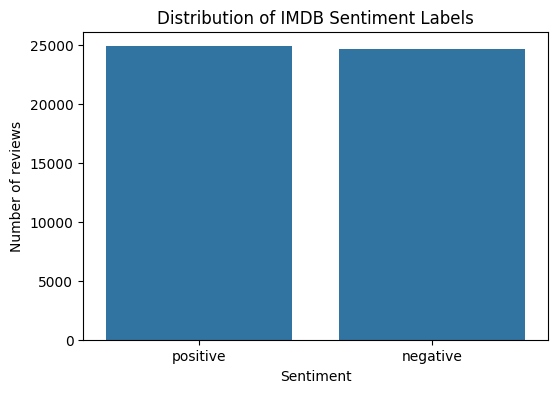
\includegraphics[width=0.82\textwidth,height=0.42\textheight,keepaspectratio]{figs/e7_9_0.png}\caption{Distribution of IMDB Sentiment Labels}\end{figure}
\Needspace{14\baselineskip}\paragraph{Output 5: X = df["review"].values}\mbox{}\\[-1ex]
\begin{Verbatim}[commandchars=\\\{\},breaklines=true,breakanywhere=true,fontsize=\scriptsize,frame=leftline,framesep=2mm,rulecolor=\color{gray}]
Training samples:   35,698
Validation samples: 3,967
Testing samples:    9,917
\end{Verbatim}
\Needspace{14\baselineskip}\paragraph{Output 6: NEURAL\_TRAIN\_LIMIT = 10000   \# Set to None to use the complete trainin}\mbox{}\\[-1ex]
\begin{Verbatim}[commandchars=\\\{\},breaklines=true,breakanywhere=true,fontsize=\scriptsize,frame=leftline,framesep=2mm,rulecolor=\color{gray}]
Neural training subset: 10000
\end{Verbatim}
\Needspace{14\baselineskip}\paragraph{Output 7: tfidf = TfidfVectorizer(}\mbox{}\\[-1ex]
\begin{Verbatim}[commandchars=\\\{\},breaklines=true,breakanywhere=true,fontsize=\scriptsize,frame=leftline,framesep=2mm,rulecolor=\color{gray}]
TF-IDF training matrix: (35698, 50000)
\end{Verbatim}
\Needspace{14\baselineskip}\paragraph{Output 8: logreg = LogisticRegression(}\mbox{}\\[-1ex]
\begin{Verbatim}[commandchars=\\\{\},breaklines=true,breakanywhere=true,fontsize=\scriptsize,frame=leftline,framesep=2mm,rulecolor=\color{gray}]
              precision    recall  f1-score   support

    negative       0.90      0.88      0.89      1976
    positive       0.88      0.91      0.90      1991

    accuracy                           0.89      3967
   macro avg       0.89      0.89      0.89      3967
weighted avg       0.89      0.89      0.89      3967
\end{Verbatim}
\Needspace{14\baselineskip}\paragraph{Output 9: PAD\_TOKEN = "<pad>"}\mbox{}\\[-1ex]
\begin{Verbatim}[commandchars=\\\{\},breaklines=true,breakanywhere=true,fontsize=\scriptsize,frame=leftline,framesep=2mm,rulecolor=\color{gray}]
Neural data loaders ready.
\end{Verbatim}
\Needspace{14\baselineskip}\paragraph{Output 10: Concatenate final forward and backward hidden states.}\mbox{}\\[-1ex]
\begin{figure}[H]\centering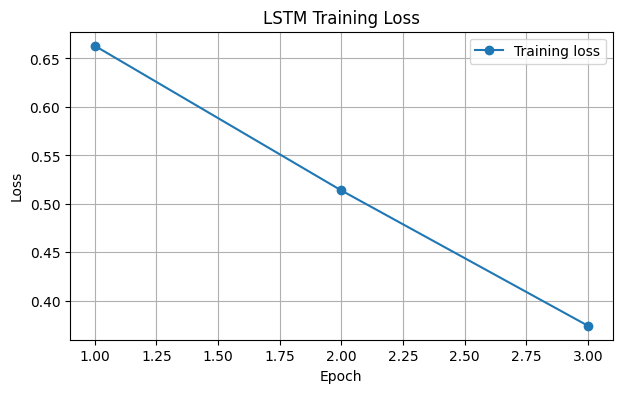
\includegraphics[width=0.82\textwidth,height=0.42\textheight,keepaspectratio]{figs/e7_24_0.png}\caption{Output figure}\end{figure}
\Needspace{14\baselineskip}\paragraph{Output 11: lstm\_y\_true, lstm\_y\_pred = predict\_torch\_model(lstm\_model, test\_loader}\mbox{}\\[-1ex]
\begin{Verbatim}[commandchars=\\\{\},breaklines=true,breakanywhere=true,fontsize=\scriptsize,frame=leftline,framesep=2mm,rulecolor=\color{gray}]
LSTM Test Metrics: \textbraceleft{}'Accuracy': 0.7682766965816276, 'Precision': 0.7487465181058496, 'Recall': 0.810126582278481, 'F1-score': 0.7782281412854661\textbraceright{}
              precision    recall  f1-score   support

    negative       0.79      0.73      0.76      4940
    positive       0.75      0.81      0.78      4977

    accuracy                           0.77      9917
   macro avg       0.77      0.77      0.77      9917
weighted avg       0.77      0.77      0.77      9917
\end{Verbatim}
\Needspace{14\baselineskip}\paragraph{Output 12: class TransformerClassifier(nn.Module):}\mbox{}\\[-1ex]
\begin{figure}[H]\centering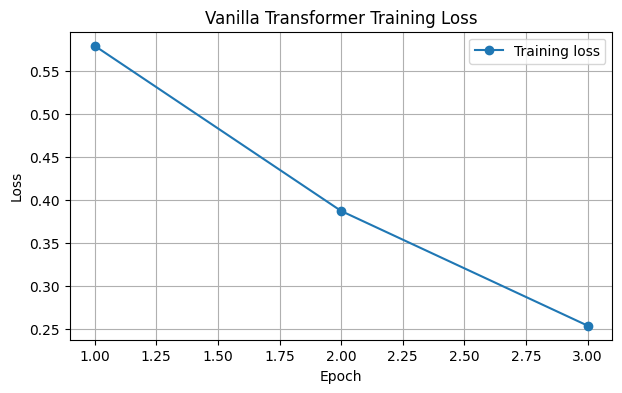
\includegraphics[width=0.82\textwidth,height=0.42\textheight,keepaspectratio]{figs/e7_28_0.png}\caption{Output figure}\end{figure}
\Needspace{14\baselineskip}\paragraph{Output 13: transformer\_y\_true, transformer\_y\_pred = predict\_torch\_model(}\mbox{}\\[-1ex]
\begin{Verbatim}[commandchars=\\\{\},breaklines=true,breakanywhere=true,fontsize=\scriptsize,frame=leftline,framesep=2mm,rulecolor=\color{gray}]
Vanilla Transformer Test Metrics: \textbraceleft{}'Accuracy': 0.8025612584450943, 'Precision': 0.7510394146016963, 'Recall': 0.9073739200321479, 'F1-score': 0.8218380345768881\textbraceright{}
              precision    recall  f1-score   support

    negative       0.88      0.70      0.78      4940
    positive       0.75      0.91      0.82      4977

    accuracy                           0.80      9917
   macro avg       0.82      0.80      0.80      9917
weighted avg       0.82      0.80      0.80      9917
\end{Verbatim}
\Needspace{14\baselineskip}\paragraph{Output 14: BERT\_MODEL\_NAME = "bert-base-uncased"}\mbox{}\\[-1ex]
\begin{Verbatim}[commandchars=\\\{\},breaklines=true,breakanywhere=true,fontsize=\scriptsize,frame=leftline,framesep=2mm,rulecolor=\color{gray}]
Key                                        | Status     |
classifier.weight                          | MISSING    |
classifier.bias                            | MISSING    |

Notes:
- MISSING:    those params were newly initialized because missing from the checkpoint. Consider training on your downstream task.
BERT training samples: 5000
BERT device: cuda
\end{Verbatim}
\Needspace{14\baselineskip}\paragraph{Output 15: class BertReviewDataset(Dataset):}\mbox{}\\[-1ex]
\begin{Verbatim}[commandchars=\\\{\},breaklines=true,breakanywhere=true,fontsize=\scriptsize,frame=leftline,framesep=2mm,rulecolor=\color{gray}]
BERT data loaders ready.
\end{Verbatim}
\Needspace{14\baselineskip}\paragraph{Output 16: def evaluate\_bert(model, loader):}\mbox{}\\[-1ex]
\begin{figure}[H]\centering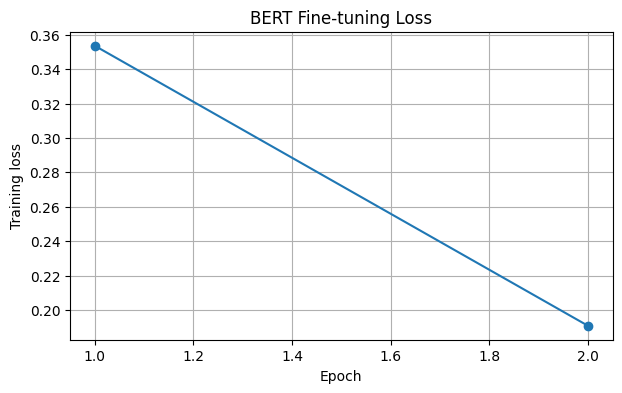
\includegraphics[width=0.82\textwidth,height=0.42\textheight,keepaspectratio]{figs/e7_36_0.png}\caption{BERT Fine-tuning Loss}\end{figure}
\Needspace{14\baselineskip}\paragraph{Output 17: bert\_y\_true, bert\_y\_pred = evaluate\_bert(bert\_model, bert\_test\_loader)}\mbox{}\\[-1ex]
\begin{Verbatim}[commandchars=\\\{\},breaklines=true,breakanywhere=true,fontsize=\scriptsize,frame=leftline,framesep=2mm,rulecolor=\color{gray}]
BERT Test Metrics: \textbraceleft{}'Accuracy': 0.8991630533427448, 'Precision': 0.8982575605848188, 'Recall': 0.9011452682338759, 'F1-score': 0.8996990972918756\textbraceright{}
              precision    recall  f1-score   support

    negative       0.90      0.90      0.90      4940
    positive       0.90      0.90      0.90      4977

    accuracy                           0.90      9917
   macro avg       0.90      0.90      0.90      9917
weighted avg       0.90      0.90      0.90      9917
\end{Verbatim}
\Needspace{14\baselineskip}\paragraph{Output 18: Logistic Regression test predictions}\mbox{}\\[-1ex]
\begin{Verbatim}[commandchars=\\\{\},breaklines=true,breakanywhere=true,fontsize=\scriptsize,frame=leftline,framesep=2mm,rulecolor=\color{gray}]
                          Accuracy  Precision  Recall  F1-score
Logistic Regression         0.9015     0.8926  0.9136    0.9030
LSTM                        0.7683     0.7487  0.8101    0.7782
Vanilla Transformer         0.8026     0.7510  0.9074    0.8218
BERT (bert-base-uncased)    0.8992     0.8983  0.9011    0.8997
\end{Verbatim}
\Needspace{14\baselineskip}\paragraph{Output 19: metrics\_to\_plot = ["Precision", "Recall", "F1-score"]}\mbox{}\\[-1ex]
\begin{figure}[H]\centering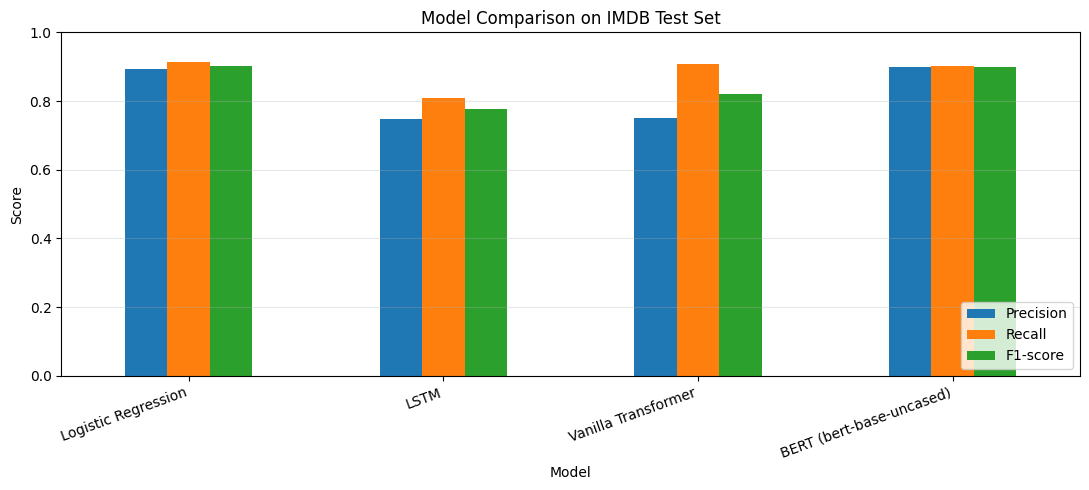
\includegraphics[width=0.82\textwidth,height=0.42\textheight,keepaspectratio]{figs/e7_42_0.png}\caption{Output figure}\end{figure}
\Needspace{14\baselineskip}\paragraph{Output 20: all\_predictions = \{}\mbox{}\\[-1ex]
\begin{figure}[H]\centering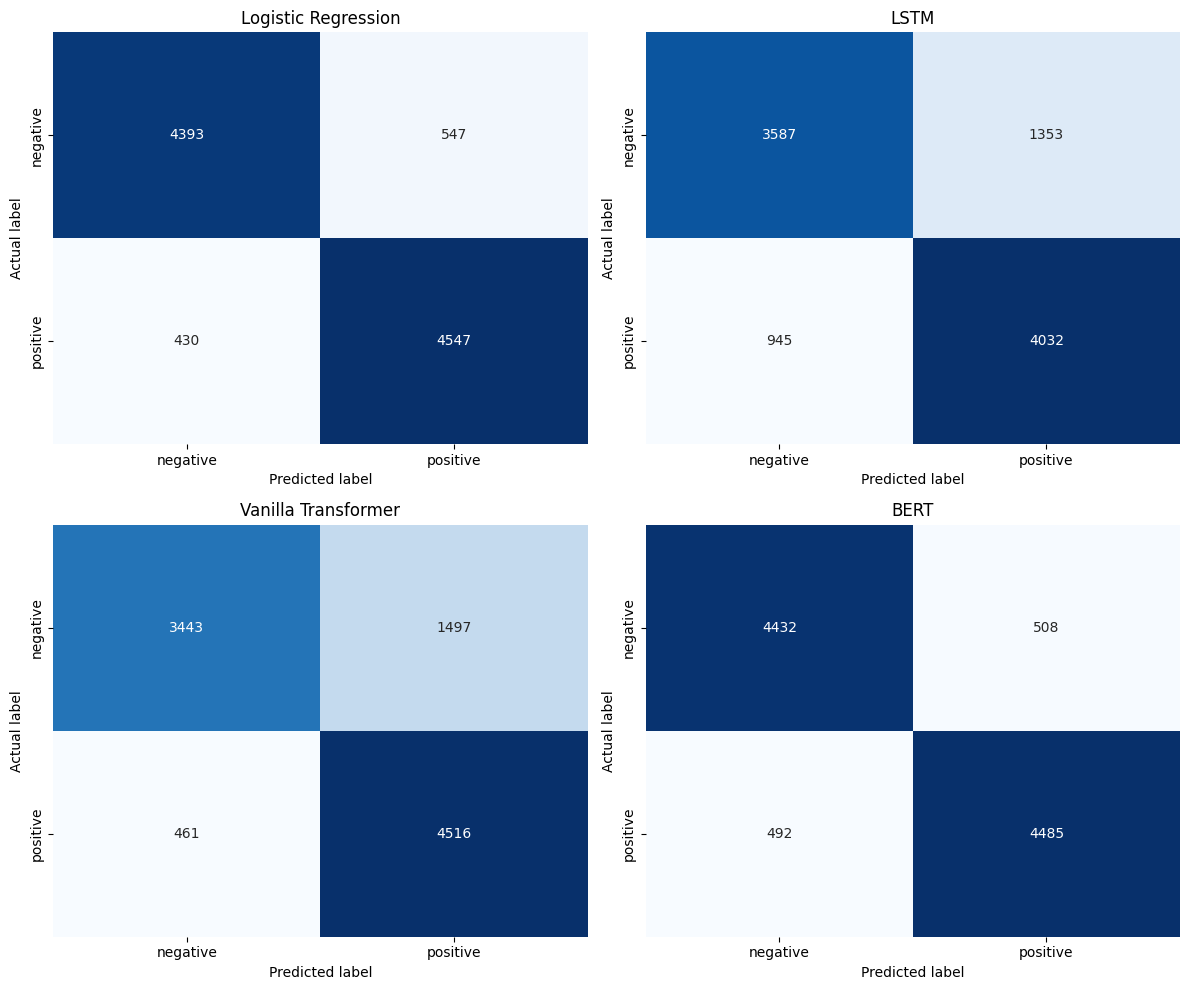
\includegraphics[width=0.82\textwidth,height=0.42\textheight,keepaspectratio]{figs/e7_44_0.png}\caption{Output figure}\end{figure}
\Needspace{14\baselineskip}\paragraph{Output 21: for model\_name, (true\_labels, predicted\_labels) in all\_predictions.ite}\mbox{}\\[-1ex]
\begin{Verbatim}[commandchars=\\\{\},breaklines=true,breakanywhere=true,fontsize=\scriptsize,frame=leftline,framesep=2mm,rulecolor=\color{gray}]
======================================================================
Logistic Regression
              precision    recall  f1-score   support

    negative       0.91      0.89      0.90      4940
    positive       0.89      0.91      0.90      4977

    accuracy                           0.90      9917
   macro avg       0.90      0.90      0.90      9917
weighted avg       0.90      0.90      0.90      9917

======================================================================
LSTM
              precision    recall  f1-score   support

    negative       0.79      0.73      0.76      4940
    positive       0.75      0.81      0.78      4977

    accuracy                           0.77      9917
   macro avg       0.77      0.77      0.77      9917
weighted avg       0.77      0.77      0.77      9917

======================================================================
Vanilla Transformer
              precision    recall  f1-score   support

    negative       0.88      0.70      0.78      4940
    positive       0.75      0.91      0.82      4977

    accuracy                           0.80      9917
   macro avg       0.82      0.80      0.80      9917
weighted avg       0.82      0.80      0.80      9917

======================================================================
BERT
              precision    recall  f1-score   support

    negative       0.90      0.90      0.90      4940
    positive       0.90      0.90      0.90      4977

    accuracy                           0.90      9917
   macro avg       0.90      0.90      0.90      9917
weighted avg       0.90      0.90      0.90      9917
\end{Verbatim}
\Needspace{14\baselineskip}\paragraph{Output 22: Logistic Regression}\mbox{}\\[-1ex]
\begin{Verbatim}[commandchars=\\\{\},breaklines=true,breakanywhere=true,fontsize=\scriptsize,frame=leftline,framesep=2mm,rulecolor=\color{gray}]
                 Model Predicted sentiment
0  Logistic Regression            Positive
1                 LSTM            Positive
2  Vanilla Transformer            Positive
3                 BERT            Positive
\end{Verbatim}
\textbf{Observations.}

\begin{longtable}[]{@{}lllll@{}}
\toprule\noalign{}
Model & Accuracy & Precision & Recall & F1 \\
\midrule\noalign{}
\endhead
\bottomrule\noalign{}
\endlastfoot
Logistic Regression & 0.9015 & 0.8926 & 0.9136 & 0.9030 \\
LSTM & 0.7683 & 0.7487 & 0.8101 & 0.7782 \\
Vanilla Transformer & 0.8026 & 0.7510 & 0.9074 & 0.8218 \\
BERT (fine-tuned) & 0.8992 & 0.8983 & 0.9011 & 0.8997 \\
\end{longtable}

\begin{itemize}
\tightlist
\item
  Logistic Regression on TF-IDF achieved the best accuracy and F1 here, with BERT essentially level (F1 0.8997 against 0.9030). The comparison is not entirely like for like: Logistic Regression used the whole training split, whereas the neural models, including BERT, were trained on only 10,000 reviews.
\item
  The from-scratch LSTM was the weakest model, and the vanilla Transformer was better than the LSTM but still around ten points below BERT, reflecting how little a small model can learn from 10,000 reviews without pretraining.
\item
  The Transformer had very high recall (0.907) but lower precision (0.751), meaning it over-predicts the positive class.
\end{itemize}


\section{Conclusion}
A well-tuned linear model on TF-IDF features is a very strong baseline for sentiment classification, and fine-tuned BERT reached the same level with a much smaller training subset. Models trained from scratch (LSTM and Transformer) lagged behind because of limited data and training time. A fair ranking would require training all models on the same amount of data.


\chapter{Experiment 8: Hindi Abstractive Text Summarization using mT5 and mBART}
\section{Abstract}
This experiment fine-tunes two multilingual sequence-to-sequence models, mT5-small and mBART-50, on a subset of the Hindi portion of the XL-Sum dataset, generates abstractive summaries, and evaluates them with ROUGE and multilingual BERTScore.


\section{Aim}
To fine-tune and compare mT5 and mBART for Hindi abstractive summarization.


\section{Objectives}
\begin{itemize}
\item Load the Hindi configuration of XL-Sum and create train, validation and test subsets.
\item Fine-tune \texttt{google/mt5-small} and \texttt{facebook/mbart-large-50-many-to-many-mmt} on the same data.
\item Evaluate summaries with ROUGE-1, ROUGE-2, ROUGE-L and mBERTScore and inspect sample outputs.
\end{itemize}

\section{Description and Theoretical Background}
Abstractive summarization generates new sentences rather than copying text from the source. mT5 is a multilingual text-to-text Transformer pretrained on a multilingual web corpus; mBART is a multilingual denoising sequence-to-sequence model. \textbf{ROUGE} measures n-gram overlap between a generated and a reference summary, while \textbf{BERTScore} compares contextual embeddings of tokens and so can reward paraphrases; the multilingual variant uses \texttt{bert-base-multilingual-cased}.


\section{Data Understanding}
XL-Sum (Hindi) provides news articles (\texttt{text}) with professionally written one-sentence summaries (\texttt{summary}). To fit the available GPU, the experiment used subsets of \textbf{2,000 training, 300 validation and 300 test} examples.


\section{Data Preprocessing}
Inputs are truncated to 512 tokens and targets to 128 tokens. mT5 uses a task prefix; mBART does not. Both models were fine-tuned for one epoch on the same subsets, with different batch sizes to fit memory.


\section{Description of the Implemented Code}
A shared \texttt{train\_one\_model} function tokenizes the data and fine-tunes either model with \texttt{Seq2SeqTrainer}; the first model's GPU memory is released before loading the second. Summaries are generated for the test subset, scored with \texttt{rouge\_score} and \texttt{bert\_score}, and the metrics and generated summaries are saved to CSV and plotted.


\section{Implemented Code}
\Needspace{8\baselineskip}\paragraph{Listing 1: XL-Sum language configuration}\mbox{}\\[-1ex]
\begin{Verbatim}[commandchars=\\\{\},breaklines=true,breakanywhere=true,fontsize=\scriptsize,frame=leftline,framesep=2mm,rulecolor=\color{gray}]
import os
import gc
import json
import random
import numpy as np
import pandas as pd
import torch
import matplotlib.pyplot as plt

from datasets import load_dataset, Dataset
from transformers import (
    AutoTokenizer,
    AutoModelForSeq2SeqLM,
    DataCollatorForSeq2Seq,
    Seq2SeqTrainingArguments,
    Seq2SeqTrainer,
    set_seed
)
from rouge_score import rouge_scorer
from bert_score import score as bert_score

SEED = 42
set_seed(SEED)
random.seed(SEED)
np.random.seed(SEED)
torch.manual_seed(SEED)

DEVICE = "cuda" if torch.cuda.is_available() else "cpu"
print("Device:", DEVICE)
if DEVICE == "cuda":
    print("GPU:", torch.cuda.get_device_name(0))

# XL-Sum language configuration
LANGUAGE = "hindi"

# Subset sizes: adjust upward for a larger experiment
TRAIN_LIMIT = 2000
VAL_LIMIT = 300
TEST_LIMIT = 300

MAX_INPUT_LENGTH = 512
MAX_TARGET_LENGTH = 128
NUM_EPOCHS = 1

# Model checkpoints
MT5_CHECKPOINT = "google/mt5-small"
MBART_CHECKPOINT = "facebook/mbart-large-50-many-to-many-mmt"

OUTPUT_DIR = "/kaggle/working/experiment8_results"
os.makedirs(OUTPUT_DIR, exist_ok=True)

print("Output directory:", OUTPUT_DIR)
\end{Verbatim}
\Needspace{8\baselineskip}\paragraph{Listing 2: Load XL-Sum Hindi directly from its Parquet files}\mbox{}\\[-1ex]
\begin{Verbatim}[commandchars=\\\{\},breaklines=true,breakanywhere=true,fontsize=\scriptsize,frame=leftline,framesep=2mm,rulecolor=\color{gray}]
from datasets import load_dataset

# Load XL-Sum Hindi directly from its Parquet files
# This works with newer Hugging Face datasets versions.

BASE_URL = "https://huggingface.co/datasets/csebuetnlp/xlsum/resolve/651dcf16e996d411b12f0bb7b8fc671788f24193/hindi/"

data_files = \textbraceleft{}
    "train": [
        BASE_URL + "xlsum-train-00000-of-00002.parquet",
        BASE_URL + "xlsum-train-00001-of-00002.parquet"
    ],
    "validation": "https://huggingface.co/datasets/csebuetnlp/xlsum/resolve/014d1559dcde03c72beff7d2e617f9792a54fd39/hindi/xlsum-validation.parquet",
    "test": BASE_URL + "xlsum-test.parquet"
\textbraceright{}

dataset = load_dataset(
    "parquet",
    data_files=data_files
)

print(dataset)

print("Available splits:", list(dataset.keys()))
print("Columns:", dataset["train"].column_names)

print("\textbackslash{}nExample article:\textbackslash{}n")
print(dataset["train"][0]["text"][:700])

print("\textbackslash{}nReference summary:\textbackslash{}n")
print(dataset["train"][0]["summary"])
\end{Verbatim}
\Needspace{8\baselineskip}\paragraph{Listing 3: The XL-Sum dataset uses 'text' for the article and 'summary' for its reference summary.}\mbox{}\\[-1ex]
\begin{Verbatim}[commandchars=\\\{\},breaklines=true,breakanywhere=true,fontsize=\scriptsize,frame=leftline,framesep=2mm,rulecolor=\color{gray}]
# The XL-Sum dataset uses 'text' for the article and 'summary' for its reference summary.
# Keep only the columns needed by this experiment.
def clean_split(split, limit):
    split = split.select(range(min(limit, len(split))))
    split = split.filter(
        lambda x: x["text"] is not None
        and x["summary"] is not None
        and len(x["text"].strip()) > 0
        and len(x["summary"].strip()) > 0
    )
    return split

train_data = clean_split(dataset["train"], TRAIN_LIMIT)
validation_data = clean_split(dataset["validation"], VAL_LIMIT)
test_data = clean_split(dataset["test"], TEST_LIMIT)

print("Training examples:", len(train_data))
print("Validation examples:", len(validation_data))
print("Test examples:", len(test_data))
\end{Verbatim}
\Needspace{8\baselineskip}\paragraph{Listing 4: mT5 expects a task prefix. mBART does not.}\mbox{}\\[-1ex]
\begin{Verbatim}[commandchars=\\\{\},breaklines=true,breakanywhere=true,fontsize=\scriptsize,frame=leftline,framesep=2mm,rulecolor=\color{gray}]
def prepare_model_data(tokenizer, model_name):
    # mT5 expects a task prefix. mBART does not.
    def preprocess(batch):
        if model_name == "mt5":
            inputs = ["summarize: " + text for text in batch["text"]]
        else:
            inputs = batch["text"]

        model_inputs = tokenizer(
            inputs,
            max_length=MAX_INPUT_LENGTH,
            truncation=True
        )

        labels = tokenizer(
            text_target=batch["summary"],
            max_length=MAX_TARGET_LENGTH,
            truncation=True
        )
        model_inputs["labels"] = labels["input_ids"]
        return model_inputs

    train_tok = train_data.map(
        preprocess, batched=True, remove_columns=train_data.column_names
    )
    val_tok = validation_data.map(
        preprocess, batched=True, remove_columns=validation_data.column_names
    )
    return train_tok, val_tok


def train_one_model(model_name, checkpoint):
    print("\textbackslash{}n" + "=" * 70)
    print("Fine-tuning:", model_name, "|", checkpoint)
    print("=" * 70)

    tokenizer = AutoTokenizer.from_pretrained(checkpoint)

    # mBART-50 requires the source and target language codes.
    if model_name == "mbart":
        tokenizer.src_lang = "hi_IN"
        tokenizer.tgt_lang = "hi_IN"

    model = AutoModelForSeq2SeqLM.from_pretrained(checkpoint)

    # Reduce memory usage, especially for mBART on a Colab T4.
    if hasattr(model, "gradient_checkpointing_enable"):
        model.gradient_checkpointing_enable()
    model.config.use_cache = False

    train_tok, val_tok = prepare_model_data(tokenizer, model_name)
    data_collator = DataCollatorForSeq2Seq(
        tokenizer=tokenizer,
        model=model,
        label_pad_token_id=-100
    )

    model_output_dir = os.path.join(OUTPUT_DIR, model_name)

    # mBART-large is memory intensive; use a smaller per-device batch.
    per_device_batch = 1 if model_name == "mbart" else 4
    grad_accumulation = 8 if model_name == "mbart" else 2

    training_args = Seq2SeqTrainingArguments(
        output_dir=model_output_dir,
        num_train_epochs=NUM_EPOCHS,
        learning_rate=5e-5,
        per_device_train_batch_size=per_device_batch,
        per_device_eval_batch_size=1 if model_name == "mbart" else 4,
        gradient_accumulation_steps=grad_accumulation,
        weight_decay=0.01,
        eval_strategy="epoch",
        save_strategy="epoch",
        logging_steps=50,
        save_total_limit=1,
        predict_with_generate=False,
        fp16=torch.cuda.is_available(),
        gradient_checkpointing=True,
        report_to="none",
        load_best_model_at_end=True,
        metric_for_best_model="eval_loss",
        greater_is_better=False
    )

    trainer = Seq2SeqTrainer(
        model=model,
        args=training_args,
        train_dataset=train_tok,
        eval_dataset=val_tok,
        data_collator=data_collator
    )

    trainer.train()
    trainer.save_model(model_output_dir)
    tokenizer.save_pretrained(model_output_dir)

    # Re-enable cache for faster generation after training.
    model.config.use_cache = True

    print("Saved fine-tuned model to:", model_output_dir)
    return model, tokenizer, model_output_dir
\end{Verbatim}
\Needspace{8\baselineskip}\paragraph{Listing 5: mt5\_model, mt5\_tokenizer, mt5\_path = train\_one\_model(}\mbox{}\\[-1ex]
\begin{Verbatim}[commandchars=\\\{\},breaklines=true,breakanywhere=true,fontsize=\scriptsize,frame=leftline,framesep=2mm,rulecolor=\color{gray}]
mt5_model, mt5_tokenizer, mt5_path = train_one_model(
    "mt5", MT5_CHECKPOINT
)
\end{Verbatim}
\Needspace{8\baselineskip}\paragraph{Listing 6: Keep the fine-tuned mT5 checkpoint on disk; release its GPU memory.}\mbox{}\\[-1ex]
\begin{Verbatim}[commandchars=\\\{\},breaklines=true,breakanywhere=true,fontsize=\scriptsize,frame=leftline,framesep=2mm,rulecolor=\color{gray}]
# Keep the fine-tuned mT5 checkpoint on disk; release its GPU memory.
del mt5_model
gc.collect()
if torch.cuda.is_available():
    torch.cuda.empty_cache()
print("GPU memory cleared where possible.")
\end{Verbatim}
\Needspace{8\baselineskip}\paragraph{Listing 7: mbart\_model, mbart\_tokenizer, mbart\_path = train\_one\_model(}\mbox{}\\[-1ex]
\begin{Verbatim}[commandchars=\\\{\},breaklines=true,breakanywhere=true,fontsize=\scriptsize,frame=leftline,framesep=2mm,rulecolor=\color{gray}]
mbart_model, mbart_tokenizer, mbart_path = train_one_model(
    "mbart", MBART_CHECKPOINT
)
\end{Verbatim}
\Needspace{8\baselineskip}\paragraph{Listing 8: def generate\_summaries(model\_path, model\_name, data, batch\_size=2):}\mbox{}\\[-1ex]
\begin{Verbatim}[commandchars=\\\{\},breaklines=true,breakanywhere=true,fontsize=\scriptsize,frame=leftline,framesep=2mm,rulecolor=\color{gray}]
def generate_summaries(model_path, model_name, data, batch_size=2):
    tokenizer = AutoTokenizer.from_pretrained(model_path)
    if model_name == "mbart":
        tokenizer.src_lang = "hi_IN"
        tokenizer.tgt_lang = "hi_IN"

    model = AutoModelForSeq2SeqLM.from_pretrained(model_path).to(DEVICE)
    model.eval()

    articles = list(data["text"])
    references = list(data["summary"])
    predictions = []

    forced_bos_token_id = None
    if model_name == "mbart":
        forced_bos_token_id = tokenizer.convert_tokens_to_ids("hi_IN")

    for start in range(0, len(articles), batch_size):
        batch_articles = articles[start:start + batch_size]
        if model_name == "mt5":
            batch_articles = ["summarize: " + x for x in batch_articles]

        inputs = tokenizer(
            batch_articles,
            return_tensors="pt",
            padding=True,
            truncation=True,
            max_length=MAX_INPUT_LENGTH
        ).to(DEVICE)

        with torch.no_grad():
            generated = model.generate(
                **inputs,
                max_length=MAX_TARGET_LENGTH,
                num_beams=4,
                early_stopping=True,
                no_repeat_ngram_size=3,
                forced_bos_token_id=forced_bos_token_id
            )

        decoded = tokenizer.batch_decode(
            generated, skip_special_tokens=True
        )
        predictions.extend(decoded)

        if (start // batch_size) % 25 == 0:
            print(f"\textbraceleft{}model_name\textbraceright{}: generated \textbraceleft{}min(start + batch_size, len(articles))\textbraceright{}/\textbraceleft{}len(articles)\textbraceright{}")

    del model
    gc.collect()
    if torch.cuda.is_available():
        torch.cuda.empty_cache()

    return predictions, references


mt5_predictions, references = generate_summaries(
    mt5_path, "mt5", test_data, batch_size=4
)

mbart_predictions, _ = generate_summaries(
    mbart_path, "mbart", test_data, batch_size=1
)

print("Generation completed.")
\end{Verbatim}
\Needspace{8\baselineskip}\paragraph{Listing 9: def calculate\_rouge(predictions, references):}\mbox{}\\[-1ex]
\begin{Verbatim}[commandchars=\\\{\},breaklines=true,breakanywhere=true,fontsize=\scriptsize,frame=leftline,framesep=2mm,rulecolor=\color{gray}]
def calculate_rouge(predictions, references):
    scorer = rouge_scorer.RougeScorer(
        ["rouge1", "rouge2", "rougeL"],
        use_stemmer=False
    )

    scores = []
    for prediction, reference in zip(predictions, references):
        result = scorer.score(reference, prediction)
        scores.append(\textbraceleft{}
            "ROUGE-1": result["rouge1"].fmeasure,
            "ROUGE-2": result["rouge2"].fmeasure,
            "ROUGE-L": result["rougeL"].fmeasure
        \textbraceright{})

    return \textbraceleft{}
        metric: float(np.mean([item[metric] for item in scores]))
        for metric in ["ROUGE-1", "ROUGE-2", "ROUGE-L"]
    \textbraceright{}


mt5_rouge = calculate_rouge(mt5_predictions, references)
mbart_rouge = calculate_rouge(mbart_predictions, references)

print("mT5 ROUGE:", mt5_rouge)
print("mBART ROUGE:", mbart_rouge)
\end{Verbatim}
\Needspace{8\baselineskip}\paragraph{Listing 10: BERTScore uses contextual multilingual embeddings to compare each generated}\mbox{}\\[-1ex]
\begin{Verbatim}[commandchars=\\\{\},breaklines=true,breakanywhere=true,fontsize=\scriptsize,frame=leftline,framesep=2mm,rulecolor=\color{gray}]
# BERTScore uses contextual multilingual embeddings to compare each generated
# summary with its reference. bert-base-multilingual-cased is the mBERT encoder.
# Run on the generated summaries from the same test subset.

def calculate_mbert_score(predictions, references):
    precision, recall, f1 = bert_score(
        cands=predictions,
        refs=references,
        model_type="bert-base-multilingual-cased",
        num_layers=12,
        batch_size=8,
        device=DEVICE,
        verbose=True,
        rescale_with_baseline=False
    )

    return \textbraceleft{}
        "mBERT-Precision": float(precision.mean().item()),
        "mBERT-Recall": float(recall.mean().item()),
        "mBERT-F1": float(f1.mean().item())
    \textbraceright{}


mt5_bert = calculate_mbert_score(mt5_predictions, references)
mbart_bert = calculate_mbert_score(mbart_predictions, references)

print("mT5 mBERTScore:", mt5_bert)
print("mBART mBERTScore:", mbart_bert)
\end{Verbatim}
\Needspace{8\baselineskip}\paragraph{Listing 11: Save numerical results}\mbox{}\\[-1ex]
\begin{Verbatim}[commandchars=\\\{\},breaklines=true,breakanywhere=true,fontsize=\scriptsize,frame=leftline,framesep=2mm,rulecolor=\color{gray}]
results = pd.DataFrame([
    \textbraceleft{}"Model": "mT5", **mt5_rouge, **mt5_bert\textbraceright{},
    \textbraceleft{}"Model": "mBART", **mbart_rouge, **mbart_bert\textbraceright{}
])

display(results.round(4))

# Save numerical results
results.to_csv(os.path.join(OUTPUT_DIR, "model_comparison.csv"), index=False)
results.to_json(
    os.path.join(OUTPUT_DIR, "model_comparison.json"),
    orient="records",
    indent=2,
    force_ascii=False
)
\end{Verbatim}
\Needspace{8\baselineskip}\paragraph{Listing 12: rouge\_columns = ["ROUGE-1", "ROUGE-2", "ROUGE-L"]}\mbox{}\\[-1ex]
\begin{Verbatim}[commandchars=\\\{\},breaklines=true,breakanywhere=true,fontsize=\scriptsize,frame=leftline,framesep=2mm,rulecolor=\color{gray}]
rouge_columns = ["ROUGE-1", "ROUGE-2", "ROUGE-L"]
results.set_index("Model")[rouge_columns].plot(
    kind="bar", figsize=(9, 5), ylim=(0, 1)
)
plt.title("ROUGE Score Comparison: mT5 vs mBART")
plt.ylabel("F1 Score")
plt.xlabel("Model")
plt.xticks(rotation=0)
plt.grid(axis="y", alpha=0.3)
plt.tight_layout()
plt.show()

bert_columns = ["mBERT-Precision", "mBERT-Recall", "mBERT-F1"]
results.set_index("Model")[bert_columns].plot(
    kind="bar", figsize=(9, 5), ylim=(0, 1)
)
plt.title("mBERTScore Comparison: mT5 vs mBART")
plt.ylabel("Score")
plt.xlabel("Model")
plt.xticks(rotation=0)
plt.grid(axis="y", alpha=0.3)
plt.tight_layout()
plt.show()
\end{Verbatim}
\Needspace{8\baselineskip}\paragraph{Listing 13: sample\_count = min(5, len(references))}\mbox{}\\[-1ex]
\begin{Verbatim}[commandchars=\\\{\},breaklines=true,breakanywhere=true,fontsize=\scriptsize,frame=leftline,framesep=2mm,rulecolor=\color{gray}]
sample_count = min(5, len(references))
for i in range(sample_count):
    print("=" * 100)
    print(f"EXAMPLE \textbraceleft{}i + 1\textbraceright{}")
    print("\textbackslash{}nARTICLE:\textbackslash{}n", test_data[i]["text"][:1000])
    print("\textbackslash{}nREFERENCE SUMMARY:\textbackslash{}n", references[i])
    print("\textbackslash{}nmT5 GENERATED SUMMARY:\textbackslash{}n", mt5_predictions[i])
    print("\textbackslash{}nmBART GENERATED SUMMARY:\textbackslash{}n", mbart_predictions[i])
    print()
\end{Verbatim}
\Needspace{8\baselineskip}\paragraph{Listing 14: comparison\_output = pd.DataFrame(\{}\mbox{}\\[-1ex]
\begin{Verbatim}[commandchars=\\\{\},breaklines=true,breakanywhere=true,fontsize=\scriptsize,frame=leftline,framesep=2mm,rulecolor=\color{gray}]
comparison_output = pd.DataFrame(\textbraceleft{}
    "article": list(test_data["text"]),
    "reference_summary": references,
    "mt5_summary": mt5_predictions,
    "mbart_summary": mbart_predictions
\textbraceright{})

summaries_path = os.path.join(OUTPUT_DIR, "generated_summaries.csv")
comparison_output.to_csv(summaries_path, index=False)

print("Saved files:")
for filename in os.listdir(OUTPUT_DIR):
    print("-", os.path.join(OUTPUT_DIR, filename))
\end{Verbatim}
\Needspace{8\baselineskip}\paragraph{Listing 15: zip\_path = shutil.make\_archive(}\mbox{}\\[-1ex]
\begin{Verbatim}[commandchars=\\\{\},breaklines=true,breakanywhere=true,fontsize=\scriptsize,frame=leftline,framesep=2mm,rulecolor=\color{gray}]
import shutil
import os

zip_path = shutil.make_archive(
    "/kaggle/working/experiment8_results",
    "zip",
    OUTPUT_DIR
)

print("ZIP created:", zip_path)
\end{Verbatim}

\section{Results and Observations}
\Needspace{14\baselineskip}\paragraph{Output 1: XL-Sum language configuration}\mbox{}\\[-1ex]
\begin{Verbatim}[commandchars=\\\{\},breaklines=true,breakanywhere=true,fontsize=\scriptsize,frame=leftline,framesep=2mm,rulecolor=\color{gray}]
  from pandas.core import (
Device: cuda
GPU: Tesla T4
Output directory: /kaggle/working/experiment8_results
\end{Verbatim}
\Needspace{14\baselineskip}\paragraph{Output 2: Load XL-Sum Hindi directly from its Parquet files}\mbox{}\\[-1ex]
\begin{Verbatim}[commandchars=\\\{\},breaklines=true,breakanywhere=true,fontsize=\scriptsize,frame=leftline,framesep=2mm,rulecolor=\color{gray}]
    train: Dataset(\textbraceleft{}
        features: ['id', 'url', 'title', 'summary', 'text'],
        num_rows: 70778
    \textbraceright{})
    validation: Dataset(\textbraceleft{}
        features: ['id', 'url', 'title', 'summary', 'text'],
        num_rows: 8847
    \textbraceright{})
    test: Dataset(\textbraceleft{}
        features: ['id', 'url', 'title', 'summary', 'text'],
        num_rows: 8847
    \textbraceright{})
\textbraceright{})
Available splits: ['train', 'validation', 'test']
Columns: ['id', 'url', 'title', 'summary', 'text']

Example article:

\hin{नेपाल} \hin{में} \hin{इस} \hin{दौरे} \hin{की} \hin{भरपूर} \hin{तैयारियां} \hin{चल} \hin{रही} \hin{हैं}. \hin{इसकी} \hin{ख़ास} \hin{वजह} \hin{भी} \hin{है} \hin{क्योंकि} 23 \hin{साल} \hin{बाद} \hin{कोई} \hin{चीनी} \hin{राष्ट्रपति} \hin{नेपाल} \hin{पहुंच} \hin{रहा} \hin{है}. \hin{नेपाल} \hin{के} \hin{प्रधानमंत्री} \hin{केपी} \hin{शर्मा} \hin{ओली} \hin{के} \hin{विदेश} \hin{मामलों} \hin{के} \hin{सलाहकार} \hin{डॉ}. \hin{राजन} \hin{भट्टाराई} \hin{ने} \hin{इस} \hin{दौरे} \hin{को} \hin{ऐतिहासिक} \hin{बताया} \hin{है}. \hin{उन्होंने} \hin{बताया} \hin{कि} \hin{चीन} \hin{के} \hin{राष्ट्रपति} \hin{के} \hin{साथ} \hin{उनका} \hin{एक} \hin{प्रतिन} ...

Reference summary:

\hin{चीन} \hin{के} \hin{राष्ट्रपति} \hin{शी} \hin{जिनपिंग} \hin{नेपाल} \hin{के} \hin{दौरे} \hin{पर} \hin{जा} \hin{रहे} \hin{हैं}. \hin{वो} 12 \hin{और} 13 \hin{अक्टूबर} \hin{को} \hin{नेपाल} \hin{में} \hin{रहेंगे}.
\end{Verbatim}
\Needspace{14\baselineskip}\paragraph{Output 3: The XL-Sum dataset uses 'text' for the article and 'summary' for its reference summary.}\mbox{}\\[-1ex]
\begin{Verbatim}[commandchars=\\\{\},breaklines=true,breakanywhere=true,fontsize=\scriptsize,frame=leftline,framesep=2mm,rulecolor=\color{gray}]
Validation examples: 300
Test examples: 300
\end{Verbatim}
\Needspace{14\baselineskip}\paragraph{Output 4: mt5\_model, mt5\_tokenizer, mt5\_path = train\_one\_model(}\mbox{}\\[-1ex]
\begin{Verbatim}[commandchars=\\\{\},breaklines=true,breakanywhere=true,fontsize=\scriptsize,frame=leftline,framesep=2mm,rulecolor=\color{gray}]
======================================================================
Fine-tuning: mt5 | google/mt5-small
======================================================================
/usr/local/lib/python3.13/dist-packages/transformers/modeling_utils.py:3195: FutureWarning: `gradient_checkpointing_enable` is deprecated and will be removed in v6. Use `activation_checkpointing_enable` instead.
/usr/local/lib/python3.13/dist-packages/transformers/training_args.py:1541: FutureWarning: `gradient_checkpointing` is deprecated and will be removed in v6. Use `activation_checkpointing` instead.
[transformers] `use_cache=True` is incompatible with gradient checkpointing. Setting `use_cache=False`.
  return super().apply(*args, **kwargs)  # type: ignore[misc]
\end{Verbatim}
\Needspace{14\baselineskip}\paragraph{Output 5: Keep the fine-tuned mT5 checkpoint on disk; release its GPU memory.}\mbox{}\\[-1ex]
\begin{Verbatim}[commandchars=\\\{\},breaklines=true,breakanywhere=true,fontsize=\scriptsize,frame=leftline,framesep=2mm,rulecolor=\color{gray}]
GPU memory cleared where possible.
\end{Verbatim}
\Needspace{14\baselineskip}\paragraph{Output 6: mbart\_model, mbart\_tokenizer, mbart\_path = train\_one\_model(}\mbox{}\\[-1ex]
\begin{Verbatim}[commandchars=\\\{\},breaklines=true,breakanywhere=true,fontsize=\scriptsize,frame=leftline,framesep=2mm,rulecolor=\color{gray}]
======================================================================
Fine-tuning: mbart | facebook/mbart-large-50-many-to-many-mmt
======================================================================
  return super().apply(*args, **kwargs)  # type: ignore[misc]
\end{Verbatim}
\Needspace{14\baselineskip}\paragraph{Output 7: def generate\_summaries(model\_path, model\_name, data, batch\_size=2):}\mbox{}\\[-1ex]
\begin{Verbatim}[commandchars=\\\{\},breaklines=true,breakanywhere=true,fontsize=\scriptsize,frame=leftline,framesep=2mm,rulecolor=\color{gray}]
mt5: generated 4/300
mt5: generated 104/300
mt5: generated 204/300
mbart: generated 26/300
mbart: generated 51/300
mbart: generated 76/300
mbart: generated 101/300
mbart: generated 126/300
mbart: generated 151/300
mbart: generated 176/300
mbart: generated 201/300
mbart: generated 226/300
mbart: generated 251/300
mbart: generated 276/300
Generation completed.
\end{Verbatim}
\Needspace{14\baselineskip}\paragraph{Output 8: def calculate\_rouge(predictions, references):}\mbox{}\\[-1ex]
\begin{Verbatim}[commandchars=\\\{\},breaklines=true,breakanywhere=true,fontsize=\scriptsize,frame=leftline,framesep=2mm,rulecolor=\color{gray}]
mT5 ROUGE: \textbraceleft{}'ROUGE-1': 0.004952380952380953, 'ROUGE-2': 0.0, 'ROUGE-L': 0.004952380952380953\textbraceright{}
mBART ROUGE: \textbraceleft{}'ROUGE-1': 0.010555555555555556, 'ROUGE-2': 0.0, 'ROUGE-L': 0.010555555555555556\textbraceright{}
\end{Verbatim}
\Needspace{14\baselineskip}\paragraph{Output 9: BERTScore uses contextual multilingual embeddings to compare each generated}\mbox{}\\[-1ex]
\begin{Verbatim}[commandchars=\\\{\},breaklines=true,breakanywhere=true,fontsize=\scriptsize,frame=leftline,framesep=2mm,rulecolor=\color{gray}]
Key                                        | Status     |  |

Notes:
Key                                        | Status     |  |

Notes:
mT5 mBERTScore: \textbraceleft{}'mBERT-Precision': 0.5227389335632324, 'mBERT-Recall': 0.5079909563064575, 'mBERT-F1': 0.5147151947021484\textbraceright{}
mBART mBERTScore: \textbraceleft{}'mBERT-Precision': 0.6249710917472839, 'mBERT-Recall': 0.574618935585022, 'mBERT-F1': 0.5974933505058289\textbraceright{}
\end{Verbatim}
\Needspace{14\baselineskip}\paragraph{Output 10: Save numerical results}\mbox{}\\[-1ex]
\begin{Verbatim}[commandchars=\\\{\},breaklines=true,breakanywhere=true,fontsize=\scriptsize,frame=leftline,framesep=2mm,rulecolor=\color{gray}]
   Model  ROUGE-1  ROUGE-2  ROUGE-L  mBERT-Precision  mBERT-Recall  mBERT-F1
0    mT5   0.0050      0.0   0.0050           0.5227        0.5080    0.5147
1  mBART   0.0106      0.0   0.0106           0.6250        0.5746    0.5975
\end{Verbatim}
\Needspace{14\baselineskip}\paragraph{Output 11: rouge\_columns = ["ROUGE-1", "ROUGE-2", "ROUGE-L"]}\mbox{}\\[-1ex]
\begin{figure}[H]\centering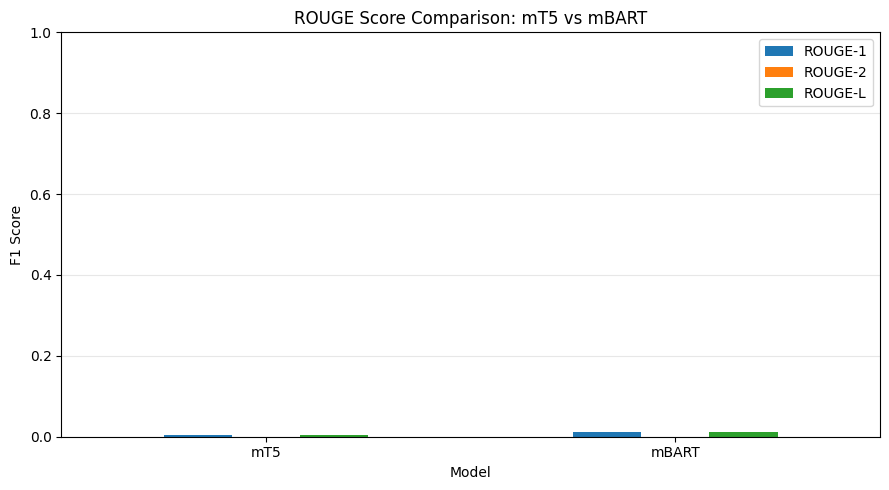
\includegraphics[width=0.82\textwidth,height=0.42\textheight,keepaspectratio]{figs/e8_26_0.png}\caption{ROUGE Score Comparison: mT5 vs mBART}\end{figure}
\begin{figure}[H]\centering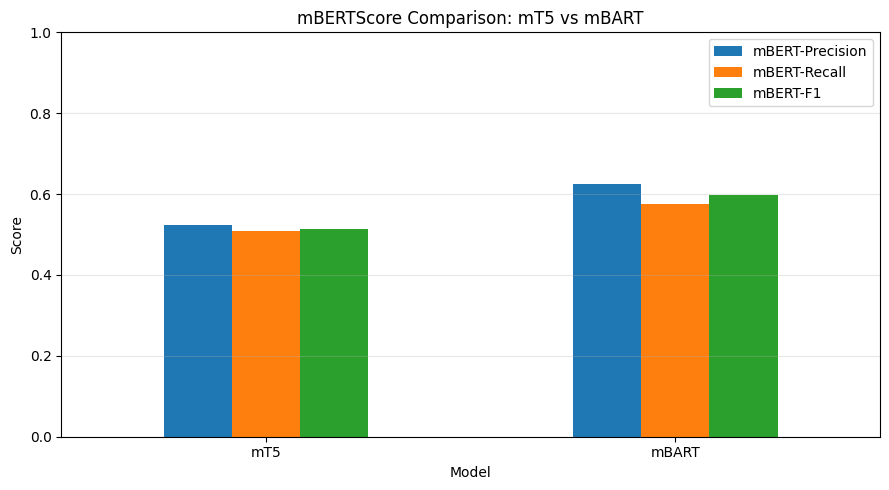
\includegraphics[width=0.82\textwidth,height=0.42\textheight,keepaspectratio]{figs/e8_26_1.png}\caption{ROUGE Score Comparison: mT5 vs mBART}\end{figure}
\Needspace{14\baselineskip}\paragraph{Output 12: sample\_count = min(5, len(references))}\mbox{}\\[-1ex]
\begin{Verbatim}[commandchars=\\\{\},breaklines=true,breakanywhere=true,fontsize=\scriptsize,frame=leftline,framesep=2mm,rulecolor=\color{gray}]
====================================================================================================
EXAMPLE 1

ARTICLE:
 \hin{नासिक} \hin{की} \hin{एक} \hin{अदालत} \hin{ने} \hin{महाराष्ट्र} \hin{पुलिस} \hin{के} \hin{आतंकवाद} \hin{निरोधक} \hin{दस्ते} (\hin{एटीएस}) \hin{के} \hin{अनुरोध} \hin{पर} \hin{ये} \hin{आदेश} \hin{दिया} \hin{है}. \hin{सरकारी} \hin{वकील} \hin{अजय} \hin{मिश्रा} \hin{ने} \hin{यह} \hin{जानकारी} \hin{दी} \hin{है}. \hin{कुछ} \hin{दिन} \hin{पहले} \hin{एटीएस} \hin{ने} \hin{मध्य} \hin{प्रदेश} \hin{के} \hin{इंदौर} \hin{शहर} \hin{से} \hin{साध्वी} \hin{प्रज्ञा} \hin{सिंह} \hin{ठाकुर} \hin{को} \hin{गिरफ़्तार} \hin{किया} \hin{था}. \hin{नासिक} \hin{की} \hin{अदालत} \hin{ने} \hin{प्रज्ञा} \hin{सिंह} \hin{और} \hin{दो} \hin{अन्य} \hin{अभियुक्तों} \hin{को} \hin{त} ...

REFERENCE SUMMARY:
 \hin{मालेगाँव} \hin{धमाकों} \hin{के} \hin{सिलसिले} \hin{में} \hin{गिरफ़्तार} \hin{साध्वी} \hin{प्रज्ञा} \hin{सिंह} \hin{ठाकुर} \hin{को} \hin{अब} \hin{पॉलीग्राफ़}, \hin{ब्रेन} \hin{मैपिंग} \hin{और} \hin{नॉर्को} \hin{टेस्ट} \hin{से} \hin{गुज़रना} \hin{होगा}. \hin{ये} \hin{सारे} \hin{टेस्ट} \hin{झूठ} \hin{पकड़ने} \hin{के} \hin{लिए} \hin{किए} \hin{जाते} \hin{हैं}.

mT5 GENERATED SUMMARY:
 <extra_id_0> \hin{के} \hin{लिए} \hin{आवेदन} \hin{है}. \hin{नासिक} \hin{की} \hin{एक} \hin{अदालत} \hin{ने} \hin{बताया} \hin{है} \hin{कि} \hin{यह} \hin{आदेश} \hin{है} \hin{कि} \hin{इसी} \hin{मामले} \hin{में} \hin{दो} \hin{पूर्व} \hin{सैनिक} \hin{अधिकारियों} \hin{को} \hin{गिरफ्तार} \hin{किया} \hin{जाना} \hin{है}.

mBART GENERATED SUMMARY:
 \hin{महाराष्ट्र} \hin{के} \hin{नासिक} \hin{में} \hin{एक} \hin{अदालत} \hin{ने} \hin{साध्वी} \hin{बुद्धि} \hin{सिंह} \hin{ठाकुर} \hin{को} \hin{गिरफ़्तार} \hin{करने} \hin{का} \hin{आदेश} \hin{दिया} \hin{है}.

====================================================================================================
EXAMPLE 2

ARTICLE:
 \hin{इस} \hin{बीच} \hin{चुनाव} \hin{आयोग} \hin{ने} \hin{शनिवार} \hin{को} \hin{राष्ट्रपति} \hin{परवेज़} \hin{मुशर्रफ़} \hin{के} \hin{नामांकन} \hin{पत्र} \hin{को} \hin{मंज़ूरी} \hin{दे} \hin{दी} \hin{है} \hin{यानी} \hin{छह} \hin{अक्तूबर} \hin{को} \hin{होने} \hin{वाले} \hin{राष्ट्रपति} \hin{पद} \hin{के} \hin{चुनाव} \hin{के} \hin{लिए} \hin{उनकी} \hin{उम्मीदवारी} \hin{पक्की} \hin{हो} \hin{गई} \hin{है}. \hin{चुनाव} \hin{आयोग} \hin{के} \hin{एक} \hin{वरिष्ठ} \hin{अधिकारी} \hin{कंवर} \hin{दिलशाद} \hin{ने} \hin{समाचार} \hin{एजेंसियों} \hin{को} \hin{बताया} \hin{कि} \hin{परवेज़} \hin{मुशर्रफ़} \hin{का} \hin{नामांकन} \hin{पत्र} \hin{सही} \hin{पा} ...

REFERENCE SUMMARY:
 \hin{पाकिस्तान} \hin{के} \hin{चुनाव} \hin{आयोग} \hin{में} \hin{शनिवार} \hin{को} \hin{राष्ट्रपति} \hin{चुनाव} \hin{के} \hin{उम्मीदवारों} \hin{के} \hin{नामांकन} \hin{पत्रों} \hin{की} \hin{जाँच} - \hin{पड़ताल} \hin{के} \hin{मौक़े} \hin{पर} \hin{इस्लामाबाद} \hin{में} \hin{आयोग} \hin{की} \hin{इमारत} \hin{के} \hin{सामने} \hin{वकीलों} \hin{और} \hin{राजनीतिक} \hin{कार्यकर्ताओं} \hin{के} \hin{प्रदर्शन} \hin{पर} \hin{पुलिस} \hin{ने} \hin{लाठी} \hin{चार्ज} \hin{किया} \hin{है} \hin{जिसमें} \hin{अनेक} \hin{लोग} \hin{घायल} \hin{हो} \hin{गए}.

mT5 GENERATED SUMMARY:
 <extra_id_0> \hin{की} \hin{उम्मीदवारी} \hin{को} \hin{मंज़ूरी} \hin{दे} \hin{दी} \hin{है}.

mBART GENERATED SUMMARY:
 \hin{पाकिस्तान} \hin{के} \hin{राष्ट्रपति} \hin{परवेज़} \hin{मुशर्रफ़} \hin{के} \hin{नामांकन} \hin{पत्र} \hin{को} \hin{मंज़ूरी} \hin{दी} \hin{गई} \hin{है}.

====================================================================================================
EXAMPLE 3

ARTICLE:
 16 \hin{महीने} \hin{के} \hin{कार्यकाल} \hin{पूरे} \hin{होने} \hin{के} \hin{बावजूद} \hin{राष्ट्रपति} \hin{मैक्रों} \hin{आर्थिक} \hin{वृद्धि} \hin{और} \hin{रोज़गार} \hin{के} \hin{वादे} \hin{को} \hin{पूरा} \hin{नहीं} \hin{कर} \hin{सके} \hin{हैं}. \hin{मैक्रों} \hin{अपने} \hin{ही} \hin{मुल्क} \hin{में} \hin{लोकप्रियता} \hin{खो} \hin{रहे} \hin{हैं}. \hin{कौन} \hin{सा} \hin{डर} \hin{मैक्रों} \hin{को} \hin{सता} \hin{रहा} \hin{है}? \hin{पोल} \hin{एजेंसियों} \hin{का} \hin{कहना} \hin{है} \hin{कि} \hin{इमैनुएल} \hin{मैक्रों} \hin{की} \hin{लोकप्रियता} \hin{सबसे} \hin{निचले} \hin{स्तर} \hin{पर} \hin{पहुंच} \hin{चुकी} \hin{है}. \hin{ओपिनियन} ...

REFERENCE SUMMARY:
 \hin{फ़्रांस} \hin{के} \hin{राष्ट्रपति} \hin{इमैनुएल} \hin{मैक्रों} \hin{की} \hin{पहचान} \hin{दुनिया} \hin{भर} \hin{में} \hin{जितनी} \hin{तेजी} \hin{से} \hin{बनी} \hin{क्या} \hin{अब} \hin{वो} \hin{मद्धम} \hin{पड़} \hin{रही} \hin{है}? \hin{क्या} \hin{फ़्रांस} \hin{में} \hin{ही} \hin{मैक्रों} \hin{जनता} \hin{का} \hin{विश्वास} \hin{दोबारा} \hin{हासिल} \hin{करने} \hin{के} \hin{लिए} \hin{संघर्ष} \hin{कर} \hin{रहे} \hin{हैं}.

mT5 GENERATED SUMMARY:
 <extra_id_0> \hin{के} \hin{मतदाताओं} \hin{की} \hin{संख्या} \hin{कम} \hin{है}. \hin{फ़्रांस} \hin{के} \hin{मतदाता} \hin{ने} \hin{कहा} \hin{है}, \hin{कि} \hin{ईरान} \hin{के} \hin{नए} \hin{ईरांस} \hin{के} \hin{लिए} \hin{चुना} \hin{है}. \hin{और} \hin{इसके} \hin{लिए} \hin{यह} \hin{है} \hin{कि} \hin{मैक्रों} \hin{की} \hin{लोकप्रियता} \hin{कम} \hin{नहीं} \hin{है}.

mBART GENERATED SUMMARY:
 \hin{अमरीका} \hin{के} \hin{राष्ट्रपति} \hin{इमैनुएल} \hin{मैक्रों} \hin{के} \hin{चुनाव} \hin{जीतने} \hin{के} \hin{बाद} \hin{क्या} \hin{हुआ} \hin{है}?

... [output truncated for length]
\end{Verbatim}
\Needspace{14\baselineskip}\paragraph{Output 13: comparison\_output = pd.DataFrame(\{}\mbox{}\\[-1ex]
\begin{Verbatim}[commandchars=\\\{\},breaklines=true,breakanywhere=true,fontsize=\scriptsize,frame=leftline,framesep=2mm,rulecolor=\color{gray}]
Saved files:
- /kaggle/working/experiment8_results/generated_summaries.csv
- /kaggle/working/experiment8_results/mbart
- /kaggle/working/experiment8_results/model_comparison.csv
- /kaggle/working/experiment8_results/mt5
- /kaggle/working/experiment8_results/model_comparison.json
\end{Verbatim}
\textbf{Observations.}

\begin{longtable}[]{@{}lllll@{}}
\toprule\noalign{}
Model & ROUGE-1 & ROUGE-2 & ROUGE-L & mBERT-F1 \\
\midrule\noalign{}
\endhead
\bottomrule\noalign{}
\endlastfoot
mT5-small & 0.0050 & 0.0000 & 0.0050 & 0.5147 \\
mBART-50 & 0.0106 & 0.0000 & 0.0106 & 0.5975 \\
\end{longtable}

\begin{itemize}
\tightlist
\item
  mBART scores higher than mT5-small on every metric reported, including mBERTScore precision, recall and F1.
\item
  The ROUGE values are close to zero for both models. This is mainly a measurement issue: the default tokenizer in the \texttt{rouge\_score} package keeps only lowercase Latin letters and digits, so Devanagari text is almost entirely discarded before overlap is computed. The mBERTScore values are therefore the more meaningful numbers for Hindi here.
\item
  Both models were trained for a single epoch on 2,000 examples, so the absolute quality is limited, and mT5-small is also a much smaller model than mBART-50.
\end{itemize}


\section{Conclusion}
mBART-50 produced better Hindi summaries than mT5-small under identical data and training budget, judged by mBERTScore. ROUGE with the default tokenizer is not suitable for Devanagari text and would need a Hindi-aware tokenizer to be informative. Larger subsets, more epochs and a larger mT5 variant would be needed for a fuller comparison.


\chapter{Experiment 9: Multiclass News Article Classification}
\section{Abstract}
Automated text categorization is a foundational discipline within Natural Language Processing (NLP), critical for news aggregation, content recommendation, and real-time information filtering. This experiment conducts a rigorous comparative benchmark of three distinct NLP modeling paradigms on the \textbf{AG's News Topic Classification Dataset}, categorizing news articles into four balanced thematic classes: \textbf{World, Sports, Business, and Science/Technology (Sci/Tech)}. The three investigated architectures encompass: (1) \textbf{Classical Machine Learning}, utilizing Term Frequency-Inverse Document Frequency (TF-IDF with unigram and bigram features, sublinear term frequency scaling) paired with a high-margin \textbf{Linear Support Vector Classifier (LinearSVC)}; (2) \textbf{Deep Learning Sequential Modeling}, utilizing a \textbf{Bidirectional Long Short-Term Memory (Bi-LSTM)} network with an embedding layer learned from scratch, spatial dropout, and dense classification layers built in TensorFlow/Keras; and (3) \textbf{Transformer-Based Transfer Learning}, fine-tuning a pretrained \textbf{DistilBERT} (\texttt{distilbert-base-uncased}) architecture with self-attention in PyTorch. The models are evaluated using a strict stratified 80\% / 10\% / 10\% split across comprehensive diagnostic criteria: \textbf{Accuracy, Macro Precision, Macro Recall, and Macro F1-Score}, alongside training duration, inference latency per sample, normalized confusion matrices, radar-chart class-wise F1 profiling, and qualitative error disagreement analysis. The results illustrate the speed-accuracy frontier across paradigms, establishing DistilBERT's contextual superiority in disambiguating semantically overlapping topics, while highlighting TF-IDF + LinearSVC as an exceptionally fast, high-performance operational baseline.

\section{Aim}
To benchmark a classical model (TF-IDF with LinearSVC), a Bi-LSTM and a fine-tuned DistilBERT on four-class news topic classification, comparing accuracy, macro F1, training time and inference latency.


\section{Objectives}
\begin{itemize}
\item Perform exploratory data analysis and text preprocessing on the AG News dataset.
\item Train three models from different paradigms on a stratified 80/10/10 split.
\item Compare models with accuracy, macro precision, recall and F1, confusion matrices and error analysis.
\end{itemize}

\section{Description and Theoretical Background}
\textbf{Approach}: Convert text to numerical vectors using \textbf{TF-IDF} (Term Frequency - Inverse Document Frequency) with unigram + bigram features, then classify with a \textbf{Linear Support Vector Classifier}.

\textbf{Why this model?}
- TF-IDF captures word importance across documents
- LinearSVC is fast, efficient, and a strong baseline for text classification
- N-gram features capture local word patterns (e.g., ``fake news'', ``stock market'')

\textbf{Approach}: Learn word embeddings from scratch, then use a \textbf{Bidirectional LSTM} to capture sequential context in both forward and backward directions.

\textbf{Why this model?}
- Word embeddings capture semantic similarity (unlike TF-IDF bag-of-words)
- Bi-LSTM processes text as a sequence, understanding word order and context
- Dropout and BatchNormalization prevent overfitting

\textbf{Approach}: Fine-tune a pretrained \textbf{DistilBERT} transformer model for sequence classification. DistilBERT is a lightweight version of BERT (40\% smaller, 60\% faster) that retains 97\% of BERT's performance.

\textbf{Why this model?}
- Pretrained on massive text corpus --- understands language deeply
- Self-attention captures long-range dependencies that LSTM struggles with
- State-of-the-art NLP performance with minimal training
- Transfer learning: leverages knowledge from billions of words

\section{Data Understanding}
The experiment uses a \textbf{30,000-article} sample of the AG News topic dataset, with columns \texttt{text} and \texttt{category} (World, Sports, Business, Sci/Tech) and no missing values. After a stratified 80/10/10 split there are 24,000 training, 3,000 validation and 3,000 test articles, with 750 test articles per class.


\section{Data Preprocessing}
Text is cleaned with a preprocessing function (lowercasing and removal of noise) before TF-IDF vectorisation (10,000 features), Keras tokenization for the Bi-LSTM and DistilBERT tokenization for the transformer.


\section{Description of the Implemented Code}
\hypertarget{end-to-end-pipeline-architecture}{%
\subsection{End-to-End Pipeline Architecture}\label{end-to-end-pipeline-architecture}}

\begin{Verbatim}[breaklines=true,breakanywhere=true,fontsize=\scriptsize,frame=leftline,framesep=2mm]
┌──────────────────────────────────────────────────────────┐
│ Input Dataset: AG News (120,000 Train / 7,600 Test)      │
│ Classes: 1-World, 2-Sports, 3-Business, 4-Sci/Tech       │
└────────────────────────────┬─────────────────────────────┘
                             │
                             ▼
┌──────────────────────────────────────────────────────────┐
│ Stage 1: Setup, Reproducibility & Data Ingestion         │
│ • Seed all PRNGs (SEED=42: NumPy, Torch, Random, TF)     │
│ • Load AG News via Hugging Face Datasets API             │
└────────────────────────────┬─────────────────────────────┘
                             │
                             ▼
┌──────────────────────────────────────────────────────────┐
│ Stage 2: Exploratory Data Analysis (EDA) & Cleaning      │
│ • Inspect class balance (pie & bar distributions)        │
│ • Analyze word count & sentence length statistics        │
│ • Generate per-class WordClouds (salient lexical cues)   │
│ • Strip HTML tags, URLs, special chars & normalize case  │
│ • Stratified Splitting: 80% Train | 10% Val | 10% Test   │
└────────────────────────────┬─────────────────────────────┘
                             │
         ┌───────────────────┼───────────────────┐
         ▼                   ▼                   ▼
┌─────────────────┐ ┌─────────────────┐ ┌─────────────────┐
│ Stage 3:        │ │ Stage 4:        │ │ Stage 5:        │
│ Model 1:        │ │ Model 2:        │ │ Model 3:        │
│ Classical ML    │ │ Deep Learning   │ │ Transformer     │
│ • TF-IDF Vector-│ │ • Keras Text-   │ │ • DistilBERT    │
│   izer (10K max │ │   Vectorization │ │   Tokenizer     │
│   features, 1-2 │ │ • Embedding     │ │ • PyTorch       │
│   n-grams)      │ │   (dim=128)     │ │   DataLoader    │
│ • LinearSVC     │ │ • Bidirectional │ │ • AdamW         │
│   (C=1.0, hinge │ │   LSTM (64 units│ │   Optimizer     │
│   loss)         │ │ • Dropout (0.3) │ │   with linear   │
│ • Sub-second    │ │ • Dense Softmax │ │   warmup        │
│   training      │ │ • Early Stopping│ │ • Sequence      │
│   execution     │ │ • Learning plots│ │   Classification│
└────────┬────────┘ └────────┬────────┘ └────────┬────────┘
         └───────────────────┼───────────────────┘
                             │
                             ▼
┌──────────────────────────────────────────────────────────┐
│ Stage 6: Benchmarking, Diagnostics & Visualizations      │
│ • Metrics: Accuracy, Macro Precision, Recall, F1-Score   │
│ • Latency Profiling: Training time & per-sample latency  │
│ • Multi-metric grouped comparative bar charts            │
│ • Side-by-side normalized confusion matrix heatmaps      │
│ • Class-wise F1 radar spider plot                        │
│ • Qualitative error analysis on model disagreements      │
│ • Interactive live inference prediction function         │
└──────────────────────────────────────────────────────────┘
\end{Verbatim}

\begin{center}\rule{0.5\linewidth}{0.5pt}\end{center}

\hypertarget{code-description-by-module}{%
\subsection{Code Description by Module}\label{code-description-by-module}}

The notebook executes a standardized multi-step machine learning pipeline:

\begin{enumerate}
\def\labelenumi{\arabic{enumi}.}
\tightlist
\item
  \textbf{Step 1: Environment Setup \& Reproducibility (Cells 1--2)}:

  \begin{itemize}
  \tightlist
  \item
    Installs \texttt{transformers}, \texttt{wordcloud}, and \texttt{datasets}.
  \item
    Imports NumPy, Pandas, Matplotlib, Seaborn, Scikit-Learn, TensorFlow, and PyTorch.
  \item
    Enforces deterministic reproducibility by setting fixed random seeds (\texttt{SEED\ =\ 42}) across all platforms.
  \end{itemize}
\item
  \textbf{Step 2: Automated Data Ingestion (Cells 3--4)}:

  \begin{itemize}
  \tightlist
  \item
    Loads the AG News corpus directly from the Hugging Face hub (\texttt{datasets.load\_dataset(\textquotesingle{}ag\_news\textquotesingle{})}).
  \item
    Converts splits into unified Pandas DataFrames with human-readable class names (\texttt{World}, \texttt{Sports}, \texttt{Business}, \texttt{Sci/Tech}).
  \end{itemize}
\item
  \textbf{Step 3: Exploratory Data Analysis (EDA) (Cells 5--10)}:

  \begin{itemize}
  \tightlist
  \item
    Evaluates class balance via combined bar and pie charts confirming uniform distribution.
  \item
    Analyzes headline and description length distributions with kernel density plots.
  \item
    Renders 4-way comparative \texttt{WordCloud} visualizations displaying the most frequent vocabulary terms per category.
  \end{itemize}
\item
  \textbf{Step 4 \& 5: Text Preprocessing \& Stratified Splitting (Cells 11--14)}:

  \begin{itemize}
  \tightlist
  \item
    Defines \texttt{clean\_text()}: strips HTML artifacts, removes web URLs, removes special punctuation, and normalizes whitespaces.
  \item
    Executes an 80\% Train, 10\% Validation, and 10\% Test stratified split using \texttt{train\_test\_split(...,\ stratify=y)}.
  \end{itemize}
\item
  \textbf{Step 6: Model 1 --- Classical ML (TF-IDF + LinearSVC) (Cells 15--16)}:

  \begin{itemize}
  \tightlist
  \item
    Transforms cleaned text into 10,000-dimensional TF-IDF feature representations using unigrams and bigrams (\texttt{ngram\_range=(1,2)}).
  \item
    Trains \texttt{LinearSVC(C=1.0)} with sub-second execution, computing validation accuracy and logging training and inference latency.
  \end{itemize}
\item
  \textbf{Step 7: Model 2 --- Deep Learning (Bi-LSTM) (Cells 17--20)}:

  \begin{itemize}
  \tightlist
  \item
    Tokenizes text using Keras \texttt{TextVectorization} (max tokens=20,000, sequence length=100).
  \item
    Builds sequential architecture: \texttt{Embedding(20000,\ 128)} \(\rightarrow\) \texttt{Bidirectional(LSTM(64,\ return\_sequences=False))} \(\rightarrow\) \texttt{Dropout(0.3)} \(\rightarrow\) \texttt{Dense(64,\ relu)} \(\rightarrow\) \texttt{Dense(4,\ softmax)}.
  \item
    Compiles with Adam optimizer and \texttt{sparse\_categorical\_crossentropy}; trains with \texttt{EarlyStopping} monitoring validation loss.
  \item
    Plots training vs.~validation loss and accuracy learning curves.
  \end{itemize}
\item
  \textbf{Step 8: Model 3 --- Pretrained Transformer (DistilBERT) (Cells 21--25)}:

  \begin{itemize}
  \tightlist
  \item
    Tokenizes sequences using \texttt{DistilBertTokenizerFast.from\_pretrained(\textquotesingle{}distilbert-base-uncased\textquotesingle{})}.
  \item
    Implements custom PyTorch \texttt{NewsDataset} yielding input IDs and attention masks.
  \item
    Loads \texttt{DistilBertForSequenceClassification} with 4 output labels and trains via PyTorch loop with AdamW optimizer, linear warmup learning rate scheduler, and gradient clipping over 3 epochs.
  \end{itemize}
\item
  \textbf{Step 9 \& 10: Multi-Model Evaluation, Visual Comparison \& Error Analysis (Cells 26--32)}:

  \begin{itemize}
  \tightlist
  \item
    Evaluates test predictions across all 3 models: Accuracy, Macro Precision, Macro Recall, and Macro F1-Score.
  \item
    Computes normalized confusion matrices plotted side-by-side (3-panel heatmap).
  \item
    Generates a per-class F1-score Radar (Spider) chart contrasting category-specific strengths.
  \item
    Performs qualitative error analysis filtering instances where models disagreed, analyzing why boundary examples (e.g.~tech business acquisitions) cause misclassifications.
  \end{itemize}
\item
  \textbf{Step 11 \& 12: Live Inference Demo \& Conclusions (Cells 33--35)}:

  \begin{itemize}
  \tightlist
  \item
    Implements \texttt{predict\_news(headline,\ content)} to accept arbitrary user inputs and output predicted category with probability confidences across all three models.
  \item
    Synthesizes computational trade-offs, accuracy ceilings, and conclusions.
  \end{itemize}
\end{enumerate}

\begin{center}\rule{0.5\linewidth}{0.5pt}\end{center}

\hypertarget{summary-of-operations-methods}{%
\subsection{Summary of Operations \& Methods}\label{summary-of-operations-methods}}

\begin{longtable}[]{@{}
  >{\raggedright\arraybackslash}p{(\columnwidth - 6\tabcolsep) * \real{0.2500}}
  >{\raggedright\arraybackslash}p{(\columnwidth - 6\tabcolsep) * \real{0.2500}}
  >{\raggedright\arraybackslash}p{(\columnwidth - 6\tabcolsep) * \real{0.2500}}
  >{\raggedright\arraybackslash}p{(\columnwidth - 6\tabcolsep) * \real{0.2500}}@{}}
\toprule\noalign{}
\begin{minipage}[b]{\linewidth}\raggedright
Step / Module
\end{minipage} & \begin{minipage}[b]{\linewidth}\raggedright
Model / Component
\end{minipage} & \begin{minipage}[b]{\linewidth}\raggedright
Core Methods \& Libraries
\end{minipage} & \begin{minipage}[b]{\linewidth}\raggedright
Primary Metric / Output
\end{minipage} \\
\midrule\noalign{}
\endhead
\bottomrule\noalign{}
\endlastfoot
\textbf{EDA \& Cleaning} & Corpus Analysis \& Preprocessing & \texttt{load\_dataset()}, regex cleaning, \texttt{WordCloud} & Length distributions, wordclouds, stratified splits \\
\textbf{Model 1} & Classical ML Baseline & \texttt{TfidfVectorizer(max\_features=10000)}, \texttt{LinearSVC()} & Accuracy, Macro F1, sub-second latency \\
\textbf{Model 2} & Bidirectional LSTM & Keras \texttt{TextVectorization}, \texttt{Bidirectional(LSTM)}, Adam & Sequential context modeling, learning curves \\
\textbf{Model 3} & DistilBERT Transformer & \texttt{DistilBertForSequenceClassification}, PyTorch AdamW & Self-attention contextual embeddings, highest F1 \\
\textbf{Evaluation} & Diagnostics \& Visualizations & \texttt{classification\_report}, \texttt{confusion\_matrix}, Radar chart & Multi-metric comparisons, 3x side-by-side confusion heatmaps \\
\textbf{Inference Demo} & Real-time Prediction & \texttt{predict\_news(headline,\ content)} & Interactive 3-model probability classification \\
\end{longtable}

\section{Implemented Code}
\Needspace{8\baselineskip}\paragraph{Listing 1: Load AG News Dataset Automatically via Hugging Face}\mbox{}\\[-1ex]
\begin{Verbatim}[commandchars=\\\{\},breaklines=true,breakanywhere=true,fontsize=\scriptsize,frame=leftline,framesep=2mm,rulecolor=\color{gray}]
# --- Load AG News Dataset Automatically via Hugging Face ---
import os
import pandas as pd
from datasets import load_dataset
from sklearn.model_selection import train_test_split

PROJECT_DIR = '/content/drive/MyDrive/NLP_Lab/Experiment-9'
os.makedirs(PROJECT_DIR, exist_ok=True)

print(" Downloading and loading AG News dataset...")
try:
    # Official namespaced HF repo for AG News
    dataset = load_dataset('fancyzhx/ag_news')
    df_train = pd.DataFrame(dataset['train'])
    df_test = pd.DataFrame(dataset['test'])
    df = pd.concat([df_train, df_test], ignore_index=True)
except Exception:
    # Direct Parquet fallback (zero HF URI dependencies)
    base_url = "https://huggingface.co/datasets/fancyzhx/ag_news/resolve/main/data"
    df_train = pd.read_parquet(f"\textbraceleft{}base_url\textbraceright{}/train-00000-of-00001.parquet")
    df_test = pd.read_parquet(f"\textbraceleft{}base_url\textbraceright{}/test-00000-of-00001.parquet")
    df = pd.concat([df_train, df_test], ignore_index=True)

# Map integer labels (0-3) to string category names so EDA & LabelEncoder work seamlessly
ag_map = \textbraceleft{}0: 'World', 1: 'Sports', 2: 'Business', 3: 'Sci/Tech'\textbraceright{}
df['category'] = df['label'].map(ag_map)
df = df[['text', 'category']]

# Stratified sample of 30,000 articles (7,500 per class) for fast Colab GPU execution
df, _ = train_test_split(df, train_size=30000, stratify=df['category'], random_state=SEED)
df = df.reset_index(drop=True)

print(f" AG News Dataset loaded successfully!")
print(f"\textbackslash{}nDataset Shape: \textbraceleft{}df.shape\textbraceright{}")
print(f" Columns: \textbraceleft{}list(df.columns)\textbraceright{}")
df.head()
\end{Verbatim}
\Needspace{8\baselineskip}\paragraph{Listing 2: Dataset overview}\mbox{}\\[-1ex]
\begin{Verbatim}[commandchars=\\\{\},breaklines=true,breakanywhere=true,fontsize=\scriptsize,frame=leftline,framesep=2mm,rulecolor=\color{gray}]
# Dataset overview
print("=" * 60)
print("DATASET OVERVIEW")
print("=" * 60)
print(f"\textbackslash{}nTotal samples: \textbraceleft{}len(df):,\textbraceright{}")
print(f"Number of features: \textbraceleft{}df.shape[1]\textbraceright{}")
print(f"\textbackslash{}nMissing values:\textbackslash{}n\textbraceleft{}df.isnull().sum()\textbraceright{}")
print(f"\textbackslash{}nData types:\textbackslash{}n\textbraceleft{}df.dtypes\textbraceright{}")
\end{Verbatim}
\Needspace{8\baselineskip}\paragraph{Listing 3: Identify text and label columns dynamically}\mbox{}\\[-1ex]
\begin{Verbatim}[commandchars=\\\{\},breaklines=true,breakanywhere=true,fontsize=\scriptsize,frame=leftline,framesep=2mm,rulecolor=\color{gray}]
# --- Identify text and label columns dynamically ---
text_cols = []
label_col = None

for col in df.columns:
    col_lower = col.lower().strip()
    if col_lower in ['category', 'label', 'class', 'target', 'topic']:
        label_col = col
    elif col_lower in ['content', 'text', 'article', 'body', 'description', 'article_content']:
        text_cols.append(col)
    elif col_lower in ['headline', 'title', 'heading']:
        text_cols.insert(0, col)  # headline first

if label_col is None:
    cat_cols = df.select_dtypes(include='object').columns
    label_col = min(cat_cols, key=lambda c: df[c].nunique())

if not text_cols:
    str_cols = df.select_dtypes(include='object').columns.drop(label_col, errors='ignore')
    text_cols = sorted(str_cols, key=lambda c: df[c].str.len().mean(), reverse=True)[:2]

print(f"Text columns: \textbraceleft{}text_cols\textbraceright{}")
print(f"Label column: \textbraceleft{}label_col\textbraceright{}")
print(f"\textbackslash{}nCategories (\textbraceleft{}df[label_col].nunique()\textbraceright{}):")
print(df[label_col].value_counts())
\end{Verbatim}
\Needspace{8\baselineskip}\paragraph{Listing 4: Class Distribution Visualization}\mbox{}\\[-1ex]
\begin{Verbatim}[commandchars=\\\{\},breaklines=true,breakanywhere=true,fontsize=\scriptsize,frame=leftline,framesep=2mm,rulecolor=\color{gray}]
# --- Class Distribution Visualization ---
fig, axes = plt.subplots(1, 2, figsize=(16, 6))

category_counts = df[label_col].value_counts()
colors = sns.color_palette("husl", len(category_counts))

bars = axes[0].bar(range(len(category_counts)), category_counts.values, color=colors)
axes[0].set_xticks(range(len(category_counts)))
axes[0].set_xticklabels(category_counts.index, rotation=45, ha='right')
axes[0].set_title('News Category Distribution', fontsize=14, fontweight='bold')
axes[0].set_ylabel('Number of Articles')
for bar, count in zip(bars, category_counts.values):
    axes[0].text(bar.get_x() + bar.get_width()/2., bar.get_height() + 50,
                f'\textbraceleft{}count:,\textbraceright{}', ha='center', va='bottom', fontsize=9)

axes[1].pie(category_counts.values, labels=category_counts.index,
            autopct='%1.1f%%', colors=colors, startangle=140)
axes[1].set_title('Category Proportions', fontsize=14, fontweight='bold')

plt.tight_layout()
plt.show()
print(f"\textbackslash{}n Class Balance Ratio (max/min): \textbraceleft{}category_counts.max()/category_counts.min():.2f\textbraceright{}")
\end{Verbatim}
\Needspace{8\baselineskip}\paragraph{Listing 5: Text Length Analysis}\mbox{}\\[-1ex]
\begin{Verbatim}[commandchars=\\\{\},breaklines=true,breakanywhere=true,fontsize=\scriptsize,frame=leftline,framesep=2mm,rulecolor=\color{gray}]
# --- Text Length Analysis ---
df['combined_text'] = df[text_cols].fillna('').agg(' '.join, axis=1)
df['word_count'] = df['combined_text'].apply(lambda x: len(str(x).split()))
df['char_count'] = df['combined_text'].apply(lambda x: len(str(x)))

fig, axes = plt.subplots(1, 2, figsize=(16, 5))

for cat in df[label_col].unique():
    subset = df[df[label_col] == cat]['word_count']
    axes[0].hist(subset, bins=50, alpha=0.5, label=cat)
axes[0].set_title('Word Count Distribution by Category', fontsize=13, fontweight='bold')
axes[0].set_xlabel('Word Count')
axes[0].set_ylabel('Frequency')
axes[0].legend(fontsize=8, loc='upper right')
axes[0].set_xlim(0, df['word_count'].quantile(0.99))

df.boxplot(column='word_count', by=label_col, ax=axes[1], rot=45)
axes[1].set_title('Word Count by Category', fontsize=13, fontweight='bold')
axes[1].set_xlabel('Category')
axes[1].set_ylabel('Word Count')
plt.suptitle('')
plt.tight_layout()
plt.show()

print(f"\textbackslash{}n Word Count Statistics:")
print(df.groupby(label_col)['word_count'].describe().round(1))
\end{Verbatim}
\Needspace{8\baselineskip}\paragraph{Listing 6: WordCloud Visualization}\mbox{}\\[-1ex]
\begin{Verbatim}[commandchars=\\\{\},breaklines=true,breakanywhere=true,fontsize=\scriptsize,frame=leftline,framesep=2mm,rulecolor=\color{gray}]
# --- WordCloud Visualization ---
top_categories = df[label_col].value_counts().head(4).index.tolist()

fig, axes = plt.subplots(2, 2, figsize=(16, 12))
axes = axes.flatten()

for idx, cat in enumerate(top_categories):
    text = ' '.join(df[df[label_col] == cat]['combined_text'].astype(str).tolist())
    wc = WordCloud(width=800, height=400, max_words=100,
                   background_color='white', colormap='viridis',
                   random_state=SEED).generate(text)
    axes[idx].imshow(wc, interpolation='bilinear')
    axes[idx].set_title(f' WordCloud: \textbraceleft{}cat\textbraceright{}', fontsize=14, fontweight='bold')
    axes[idx].axis('off')

plt.suptitle('Word Clouds for Top 4 News Categories', fontsize=16, fontweight='bold', y=1.02)
plt.tight_layout()
plt.show()
\end{Verbatim}
\Needspace{8\baselineskip}\paragraph{Listing 7: Text Preprocessing Pipeline}\mbox{}\\[-1ex]
\begin{Verbatim}[commandchars=\\\{\},breaklines=true,breakanywhere=true,fontsize=\scriptsize,frame=leftline,framesep=2mm,rulecolor=\color{gray}]
# --- Text Preprocessing Pipeline ---
def clean_text(text):
    """Clean and normalize text for NLP processing."""
    if not isinstance(text, str):
        return ""
    text = re.sub(r'<[^>]+>', '', text)           # Remove HTML tags
    text = re.sub(r'http\textbackslash{}S+|www\textbackslash{}.\textbackslash{}S+', '', text)  # Remove URLs
    text = re.sub(r'\textbackslash{}S+@\textbackslash{}S+', '', text)            # Remove emails
    text = re.sub(r'[^a-zA-Z\textbackslash{}s]', ' ', text)       # Keep only letters
    text = re.sub(r'\textbackslash{}s+', ' ', text).strip()        # Remove extra whitespace
    text = text.lower()
    return text

print(" Cleaning text data...")
df['clean_text'] = df['combined_text'].apply(clean_text)

# Remove empty rows
before_len = len(df)
df = df[df['clean_text'].str.len() > 10].reset_index(drop=True)
print(f"   Removed \textbraceleft{}before_len - len(df)\textbraceright{} empty/very short rows")

# Encode labels
le = LabelEncoder()
df['label_encoded'] = le.fit_transform(df[label_col])

label_mapping = dict(zip(le.classes_, le.transform(le.classes_)))
print(f"\textbackslash{}n Label Encoding:")
for name, idx in label_mapping.items():
    print(f"   \textbraceleft{}idx\textbraceright{}: \textbraceleft{}name\textbraceright{}")

print(f"\textbackslash{}n Preprocessing complete! Dataset size: \textbraceleft{}len(df):,\textbraceright{} samples")
print(f"   Clean text sample: '\textbraceleft{}df['clean_text'].iloc[0][:100]\textbraceright{}...'")
\end{Verbatim}
\Needspace{8\baselineskip}\paragraph{Listing 8: Stratified Train/Validation/Test Split}\mbox{}\\[-1ex]
\begin{Verbatim}[commandchars=\\\{\},breaklines=true,breakanywhere=true,fontsize=\scriptsize,frame=leftline,framesep=2mm,rulecolor=\color{gray}]
# --- Stratified Train/Validation/Test Split ---
X = df['clean_text'].values
y = df['label_encoded'].values

# Step 1: 80% Train, 20% Temp
X_train, X_temp, y_train, y_temp = train_test_split(
    X, y, test_size=0.20, stratify=y, random_state=SEED
)

# Step 2: 50/50 split of Temp -> 10% Val, 10% Test
X_val, X_test, y_val, y_test = train_test_split(
    X_temp, y_temp, test_size=0.50, stratify=y_temp, random_state=SEED
)

total = len(X)
print("=" * 60)
print("DATASET SPLIT VERIFICATION")
print("=" * 60)
print(f"\textbackslash{}n Total samples: \textbraceleft{}total:,\textbraceright{}")
print(f"   Training:   \textbraceleft{}len(X_train):,\textbraceright{} (\textbraceleft{}len(X_train)/total*100:.1f\textbraceright{}%)")
print(f"   Validation: \textbraceleft{}len(X_val):,\textbraceright{} (\textbraceleft{}len(X_val)/total*100:.1f\textbraceright{}%)")
print(f"   Test:       \textbraceleft{}len(X_test):,\textbraceright{} (\textbraceleft{}len(X_test)/total*100:.1f\textbraceright{}%)")

# Verify class distribution
fig, axes = plt.subplots(1, 3, figsize=(18, 5))
split_names = ['Training Set', 'Validation Set', 'Test Set']
split_labels = [y_train, y_val, y_test]

for ax, name, labels in zip(axes, split_names, split_labels):
    unique, counts = np.unique(labels, return_counts=True)
    class_names = le.inverse_transform(unique)
    bars = ax.bar(class_names, counts / len(labels) * 100,
                  color=sns.color_palette("husl", len(unique)))
    ax.set_title(f'\textbraceleft{}name\textbraceright{}\textbackslash{}n(n=\textbraceleft{}len(labels):,\textbraceright{})', fontsize=12, fontweight='bold')
    ax.set_ylabel('Percentage (%)')
    ax.set_ylim(0, max(counts / len(labels) * 100) * 1.3)
    ax.tick_params(axis='x', rotation=45)
    for bar, pct in zip(bars, counts / len(labels) * 100):
        ax.text(bar.get_x() + bar.get_width()/2., bar.get_height() + 0.3,
                f'\textbraceleft{}pct:.1f\textbraceright{}%', ha='center', va='bottom', fontsize=8)

plt.suptitle(' Stratified Split: Class Distribution Consistency', fontsize=14, fontweight='bold')
plt.tight_layout()
plt.show()
print("\textbackslash{}n Class proportions are consistent across all 3 splits!")
\end{Verbatim}
\Needspace{8\baselineskip}\paragraph{Listing 9: MODEL 1: TF-IDF + Linear SVC}\mbox{}\\[-1ex]
\begin{Verbatim}[commandchars=\\\{\},breaklines=true,breakanywhere=true,fontsize=\scriptsize,frame=leftline,framesep=2mm,rulecolor=\color{gray}]
# ============================================================
# MODEL 1: TF-IDF + Linear SVC
# ============================================================
print("=" * 60)
print("MODEL 1: TF-IDF + LinearSVC")
print("=" * 60)

# --- TF-IDF Vectorization ---
tfidf = TfidfVectorizer(
    max_features=10000,
    ngram_range=(1, 2),
    sublinear_tf=True,
    stop_words='english',
    max_df=0.95,
    min_df=2
)

print(" Fitting TF-IDF vectorizer...")
X_train_tfidf = tfidf.fit_transform(X_train)
X_val_tfidf = tfidf.transform(X_val)
X_test_tfidf = tfidf.transform(X_test)
print(f"   Vocabulary size: \textbraceleft{}len(tfidf.vocabulary_):,\textbraceright{}")
print(f"   Feature matrix shape: \textbraceleft{}X_train_tfidf.shape\textbraceright{}")

# --- Train ---
print("\textbackslash{}n Training LinearSVC...")
start_time = time.time()
base_svc = LinearSVC(C=1.0, max_iter=2000, random_state=SEED)
model1 = CalibratedClassifierCV(base_svc, cv=3)
model1.fit(X_train_tfidf, y_train)
model1_train_time = time.time() - start_time
print(f"   Training completed in \textbraceleft{}model1_train_time:.2f\textbraceright{} seconds")

# --- Validation ---
val_pred1 = model1.predict(X_val_tfidf)
val_acc1 = accuracy_score(y_val, val_pred1)
print(f"\textbackslash{}n Validation Accuracy: \textbraceleft{}val_acc1:.4f\textbraceright{}")

# --- Test ---
start_time = time.time()
test_pred1 = model1.predict(X_test_tfidf)
model1_inference_time = (time.time() - start_time) / len(X_test) * 1000

test_acc1 = accuracy_score(y_test, test_pred1)
test_f1_1 = f1_score(y_test, test_pred1, average='macro')

print(f"\textbackslash{}n Test Results:")
print(f"   Accuracy:  \textbraceleft{}test_acc1:.4f\textbraceright{}")
print(f"   Macro F1:  \textbraceleft{}test_f1_1:.4f\textbraceright{}")
print(f"   Inference:  \textbraceleft{}model1_inference_time:.3f\textbraceright{} ms/sample")
print(f"\textbackslash{}n Classification Report:")
print(classification_report(y_test, test_pred1, target_names=le.classes_))

# Confusion Matrix
cm1 = confusion_matrix(y_test, test_pred1)
plt.figure(figsize=(10, 8))
sns.heatmap(cm1, annot=True, fmt='d', cmap='Blues',
            xticklabels=le.classes_, yticklabels=le.classes_)
plt.title('Model 1: TF-IDF + LinearSVC — Confusion Matrix', fontsize=14, fontweight='bold')
plt.xlabel('Predicted')
plt.ylabel('Actual')
plt.xticks(rotation=45, ha='right')
plt.yticks(rotation=0)
plt.tight_layout()
plt.show()
\end{Verbatim}
\Needspace{8\baselineskip}\paragraph{Listing 10: MODEL 2: Bi-LSTM with Word Embeddings (TensorFlow/Keras)}\mbox{}\\[-1ex]
\begin{Verbatim}[commandchars=\\\{\},breaklines=true,breakanywhere=true,fontsize=\scriptsize,frame=leftline,framesep=2mm,rulecolor=\color{gray}]
# ============================================================
# MODEL 2: Bi-LSTM with Word Embeddings (TensorFlow/Keras)
# ============================================================
print("=" * 60)
print("MODEL 2: Bidirectional LSTM")
print("=" * 60)

VOCAB_SIZE = 20000
MAX_LENGTH = 150
EMBEDDING_DIM = 128
LSTM_UNITS = 64
BATCH_SIZE = 64
EPOCHS = 15

# --- Text Vectorization ---
print(" Building text vectorizer...")
text_vectorizer = layers.TextVectorization(
    max_tokens=VOCAB_SIZE,
    output_mode='int',
    output_sequence_length=MAX_LENGTH
)
text_vectorizer.adapt(X_train)
print(f"   Vocabulary size: \textbraceleft{}text_vectorizer.vocabulary_size()\textbraceright{}")

# --- Build Model ---
print("\textbackslash{}n Building Bi-LSTM model...")
num_classes = len(le.classes_)

model2 = keras.Sequential([
    keras.Input(shape=(1,), dtype=tf.string),
    text_vectorizer,
    layers.Embedding(VOCAB_SIZE, EMBEDDING_DIM, mask_zero=True),
    layers.SpatialDropout1D(0.2),
    layers.Bidirectional(layers.LSTM(LSTM_UNITS, return_sequences=False)),
    layers.BatchNormalization(),
    layers.Dense(64, activation='relu'),
    layers.Dropout(0.3),
    layers.Dense(num_classes, activation='softmax')
])

model2.compile(
    optimizer=keras.optimizers.Adam(learning_rate=1e-3),
    loss='sparse_categorical_crossentropy',
    metrics=['accuracy']
)

model2.summary()

# --- Callbacks ---
callbacks = [
    keras.callbacks.EarlyStopping(
        monitor='val_loss', patience=3,
        restore_best_weights=True, verbose=1
    ),
    keras.callbacks.ReduceLROnPlateau(
        monitor='val_loss', factor=0.5,
        praise=2, min_lr=1e-6, verbose=1
    )
]

# --- Train ---
print("\textbackslash{}n Training Bi-LSTM...")
start_time = time.time()

history = model2.fit(
    X_train, y_train,
    validation_data=(X_val, y_val),
    epochs=EPOCHS,
    batch_size=BATCH_SIZE,
    callbacks=callbacks,
    verbose=1
)

model2_train_time = time.time() - start_time
print(f"\textbackslash{}n Training completed in \textbraceleft{}model2_train_time:.1f\textbraceright{} seconds")
\end{Verbatim}
\Needspace{8\baselineskip}\paragraph{Listing 11: Learning Curves}\mbox{}\\[-1ex]
\begin{Verbatim}[commandchars=\\\{\},breaklines=true,breakanywhere=true,fontsize=\scriptsize,frame=leftline,framesep=2mm,rulecolor=\color{gray}]
# --- Learning Curves ---
fig, axes = plt.subplots(1, 2, figsize=(14, 5))

axes[0].plot(history.history['loss'], label='Train Loss', linewidth=2)
axes[0].plot(history.history['val_loss'], label='Val Loss', linewidth=2)
axes[0].set_title('Model 2: Training vs Validation Loss', fontsize=13, fontweight='bold')
axes[0].set_xlabel('Epoch')
axes[0].set_ylabel('Loss')
axes[0].legend()
axes[0].grid(True, alpha=0.3)

axes[1].plot(history.history['accuracy'], label='Train Accuracy', linewidth=2)
axes[1].plot(history.history['val_accuracy'], label='Val Accuracy', linewidth=2)
axes[1].set_title('Model 2: Training vs Validation Accuracy', fontsize=13, fontweight='bold')
axes[1].set_xlabel('Epoch')
axes[1].set_ylabel('Accuracy')
axes[1].legend()
axes[1].grid(True, alpha=0.3)

plt.tight_layout()
plt.show()
\end{Verbatim}
\Needspace{8\baselineskip}\paragraph{Listing 12: Bi-LSTM Test Evaluation}\mbox{}\\[-1ex]
\begin{Verbatim}[commandchars=\\\{\},breaklines=true,breakanywhere=true,fontsize=\scriptsize,frame=leftline,framesep=2mm,rulecolor=\color{gray}]
# --- Bi-LSTM Test Evaluation ---
start_time = time.time()
test_pred2_probs = model2.predict(X_test, verbose=0)
model2_inference_time = (time.time() - start_time) / len(X_test) * 1000

test_pred2 = np.argmax(test_pred2_probs, axis=1)
test_acc2 = accuracy_score(y_test, test_pred2)
test_f1_2 = f1_score(y_test, test_pred2, average='macro')

print(" Test Results:")
print(f"   Accuracy:  \textbraceleft{}test_acc2:.4f\textbraceright{}")
print(f"   Macro F1:  \textbraceleft{}test_f1_2:.4f\textbraceright{}")
print(f"   Inference:  \textbraceleft{}model2_inference_time:.3f\textbraceright{} ms/sample")
print(f"\textbackslash{}n Classification Report:")
print(classification_report(y_test, test_pred2, target_names=le.classes_))

cm2 = confusion_matrix(y_test, test_pred2)
plt.figure(figsize=(10, 8))
sns.heatmap(cm2, annot=True, fmt='d', cmap='Greens',
            xticklabels=le.classes_, yticklabels=le.classes_)
plt.title('Model 2: Bi-LSTM — Confusion Matrix', fontsize=14, fontweight='bold')
plt.xlabel('Predicted')
plt.ylabel('Actual')
plt.xticks(rotation=45, ha='right')
plt.yticks(rotation=0)
plt.tight_layout()
plt.show()
\end{Verbatim}
\Needspace{8\baselineskip}\paragraph{Listing 13: MODEL 3: Fine-tuned DistilBERT}\mbox{}\\[-1ex]
\begin{Verbatim}[commandchars=\\\{\},breaklines=true,breakanywhere=true,fontsize=\scriptsize,frame=leftline,framesep=2mm,rulecolor=\color{gray}]
# ============================================================
# MODEL 3: Fine-tuned DistilBERT
# ============================================================
print("=" * 60)
print("MODEL 3: DistilBERT (Fine-tuned Transformer)")
print("=" * 60)

MODEL_NAME = 'distilbert-base-uncased'
MAX_LEN = 128

print(f" Loading tokenizer: \textbraceleft{}MODEL_NAME\textbraceright{}")
tokenizer = AutoTokenizer.from_pretrained(MODEL_NAME)

# --- Tokenize Data ---
print(" Tokenizing datasets...")

def tokenize_batch(texts, max_len=MAX_LEN):
    return tokenizer(
        texts.tolist() if hasattr(texts, 'tolist') else list(texts),
        padding='max_length',
        truncation=True,
        max_length=max_len,
        return_tensors='pt'
    )

train_encodings = tokenize_batch(X_train)
val_encodings = tokenize_batch(X_val)
test_encodings = tokenize_batch(X_test)

print(f"   Tokenization complete")
print(f"   Input IDs shape: \textbraceleft{}train_encodings['input_ids'].shape\textbraceright{}")
\end{Verbatim}
\Needspace{8\baselineskip}\paragraph{Listing 14: PyTorch Dataset}\mbox{}\\[-1ex]
\begin{Verbatim}[commandchars=\\\{\},breaklines=true,breakanywhere=true,fontsize=\scriptsize,frame=leftline,framesep=2mm,rulecolor=\color{gray}]
# --- PyTorch Dataset ---
class NewsDataset(Dataset):
    def __init__(self, encodings, labels):
        self.encodings = encodings
        self.labels = torch.tensor(labels, dtype=torch.long)

    def __len__(self):
        return len(self.labels)

    def __getitem__(self, idx):
        return \textbraceleft{}
            'input_ids': self.encodings['input_ids'][idx],
            'attention_mask': self.encodings['attention_mask'][idx],
            'labels': self.labels[idx]
        \textbraceright{}

train_dataset = NewsDataset(train_encodings, y_train)
val_dataset = NewsDataset(val_encodings, y_val)
test_dataset = NewsDataset(test_encodings, y_test)

BATCH_SIZE_BERT = 32
train_loader = DataLoader(train_dataset, batch_size=BATCH_SIZE_BERT, shuffle=True)
val_loader = DataLoader(val_dataset, batch_size=BATCH_SIZE_BERT)
test_loader = DataLoader(test_dataset, batch_size=BATCH_SIZE_BERT)

print(f"   DataLoaders created")
print(f"   Train batches: \textbraceleft{}len(train_loader)\textbraceright{}")
print(f"   Val batches:   \textbraceleft{}len(val_loader)\textbraceright{}")
print(f"   Test batches:  \textbraceleft{}len(test_loader)\textbraceright{}")
\end{Verbatim}
\Needspace{8\baselineskip}\paragraph{Listing 15: Load \& Fine-tune DistilBERT}\mbox{}\\[-1ex]
\begin{Verbatim}[commandchars=\\\{\},breaklines=true,breakanywhere=true,fontsize=\scriptsize,frame=leftline,framesep=2mm,rulecolor=\color{gray}]
# --- Load & Fine-tune DistilBERT ---
print(f" Loading \textbraceleft{}MODEL_NAME\textbraceright{} for sequence classification...")
num_classes = len(le.classes_)
model3 = AutoModelForSequenceClassification.from_pretrained(
    MODEL_NAME, num_labels=num_classes
).to(DEVICE)

total_params = sum(p.numel() for p in model3.parameters())
trainable_params = sum(p.numel() for p in model3.parameters() if p.requires_grad)
print(f"   Total parameters: \textbraceleft{}total_params:,\textbraceright{}")
print(f"   Trainable parameters: \textbraceleft{}trainable_params:,\textbraceright{}")

EPOCHS_BERT = 3
LR = 3e-5
optimizer = AdamW(model3.parameters(), lr=LR, weight_decay=0.01)
total_steps = len(train_loader) * EPOCHS_BERT
scheduler = LinearLR(optimizer, start_factor=1.0, end_factor=0.0, total_iters=total_steps)
loss_fn = torch.nn.CrossEntropyLoss()

print(f"\textbackslash{}n Training DistilBERT for \textbraceleft{}EPOCHS_BERT\textbraceright{} epochs...")
start_time = time.time()
train_losses, val_losses, val_accuracies = [], [], []

for epoch in range(EPOCHS_BERT):
    model3.train()
    epoch_loss, correct, total_samples = 0, 0, 0

    for batch_idx, batch in enumerate(train_loader):
        input_ids = batch['input_ids'].to(DEVICE)
        attention_mask = batch['attention_mask'].to(DEVICE)
        labels = batch['labels'].to(DEVICE)

        optimizer.zero_grad()
        outputs = model3(input_ids=input_ids, attention_mask=attention_mask)
        loss = loss_fn(outputs.logits, labels)
        loss.backward()
        torch.nn.utils.clip_grad_norm_(model3.parameters(), 1.0)
        optimizer.step()
        scheduler.step()

        epoch_loss += loss.item()
        preds = torch.argmax(outputs.logits, dim=1)
        correct += (preds == labels).sum().item()
        total_samples += len(labels)

        if (batch_idx + 1) % 50 == 0:
            print(f"   Epoch \textbraceleft{}epoch+1\textbraceright{}/\textbraceleft{}EPOCHS_BERT\textbraceright{} | Batch \textbraceleft{}batch_idx+1\textbraceright{}/\textbraceleft{}len(train_loader)\textbraceright{} | Loss: \textbraceleft{}loss.item():.4f\textbraceright{}")

    train_loss = epoch_loss / len(train_loader)
    train_acc = correct / total_samples
    train_losses.append(train_loss)

    # Validation
    model3.eval()
    val_loss, val_correct, val_total = 0, 0, 0
    with torch.no_grad():
        for batch in val_loader:
            input_ids = batch['input_ids'].to(DEVICE)
            attention_mask = batch['attention_mask'].to(DEVICE)
            labels = batch['labels'].to(DEVICE)
            outputs = model3(input_ids=input_ids, attention_mask=attention_mask)
            loss = loss_fn(outputs.logits, labels)
            val_loss += loss.item()
            preds = torch.argmax(outputs.logits, dim=1)
            val_correct += (preds == labels).sum().item()
            val_total += len(labels)

    val_loss = val_loss / len(val_loader)
    val_acc = val_correct / val_total
    val_losses.append(val_loss)
    val_accuracies.append(val_acc)

    print(f"\textbackslash{}n   Epoch \textbraceleft{}epoch+1\textbraceright{}/\textbraceleft{}EPOCHS_BERT\textbraceright{}: Train Loss=\textbraceleft{}train_loss:.4f\textbraceright{} | Train Acc=\textbraceleft{}train_acc:.4f\textbraceright{} | Val Loss=\textbraceleft{}val_loss:.4f\textbraceright{} | Val Acc=\textbraceleft{}val_acc:.4f\textbraceright{}")

model3_train_time = time.time() - start_time
print(f"\textbackslash{}n Training completed in \textbraceleft{}model3_train_time:.1f\textbraceright{} seconds (\textbraceleft{}model3_train_time/60:.1f\textbraceright{} min)")
\end{Verbatim}
\Needspace{8\baselineskip}\paragraph{Listing 16: DistilBERT Test Evaluation}\mbox{}\\[-1ex]
\begin{Verbatim}[commandchars=\\\{\},breaklines=true,breakanywhere=true,fontsize=\scriptsize,frame=leftline,framesep=2mm,rulecolor=\color{gray}]
# --- DistilBERT Test Evaluation ---
print("\textbackslash{}n Evaluating on Test Set...")
model3.eval()
all_preds, all_labels = [], []

start_time = time.time()
with torch.no_grad():
    for batch in test_loader:
        input_ids = batch['input_ids'].to(DEVICE)
        attention_mask = batch['attention_mask'].to(DEVICE)
        labels = batch['labels']
        outputs = model3(input_ids=input_ids, attention_mask=attention_mask)
        preds = torch.argmax(outputs.logits, dim=1).cpu().numpy()
        all_preds.extend(preds)
        all_labels.extend(labels.numpy())

model3_inference_time = (time.time() - start_time) / len(X_test) * 1000
test_pred3 = np.array(all_preds)
test_acc3 = accuracy_score(y_test, test_pred3)
test_f1_3 = f1_score(y_test, test_pred3, average='macro')

print(f"   Accuracy:  \textbraceleft{}test_acc3:.4f\textbraceright{}")
print(f"   Macro F1:  \textbraceleft{}test_f1_3:.4f\textbraceright{}")
print(f"   Inference:  \textbraceleft{}model3_inference_time:.3f\textbraceright{} ms/sample")
print(f"\textbackslash{}n Classification Report:")
print(classification_report(y_test, test_pred3, target_names=le.classes_))

# Confusion Matrix
cm3 = confusion_matrix(y_test, test_pred3)
plt.figure(figsize=(10, 8))
sns.heatmap(cm3, annot=True, fmt='d', cmap='Oranges',
            xticklabels=le.classes_, yticklabels=le.classes_)
plt.title('Model 3: DistilBERT — Confusion Matrix', fontsize=14, fontweight='bold')
plt.xlabel('Predicted')
plt.ylabel('Actual')
plt.xticks(rotation=45, ha='right')
plt.yticks(rotation=0)
plt.tight_layout()
plt.show()
\end{Verbatim}
\Needspace{8\baselineskip}\paragraph{Listing 17: COMPREHENSIVE MODEL COMPARISON}\mbox{}\\[-1ex]
\begin{Verbatim}[commandchars=\\\{\},breaklines=true,breakanywhere=true,fontsize=\scriptsize,frame=leftline,framesep=2mm,rulecolor=\color{gray}]
# ============================================================
# COMPREHENSIVE MODEL COMPARISON
# ============================================================
print("=" * 60)
print("COMPREHENSIVE MODEL COMPARISON")
print("=" * 60)

results = \textbraceleft{}
    'Model': ['TF-IDF + LinearSVC', 'Bi-LSTM', 'DistilBERT'],
    'Paradigm': ['Classical ML', 'Deep Learning', 'Transformer'],
    'Test Accuracy': [test_acc1, test_acc2, test_acc3],
    'Macro Precision': [
        precision_score(y_test, test_pred1, average='macro'),
        precision_score(y_test, test_pred2, average='macro'),
        precision_score(y_test, test_pred3, average='macro')
    ],
    'Macro Recall': [
        recall_score(y_test, test_pred1, average='macro'),
        recall_score(y_test, test_pred2, average='macro'),
        recall_score(y_test, test_pred3, average='macro')
    ],
    'Macro F1': [test_f1_1, test_f1_2, test_f1_3],
    'Training Time (s)': [model1_train_time, model2_train_time, model3_train_time],
    'Inference (ms/sample)': [model1_inference_time, model2_inference_time, model3_inference_time]
\textbraceright{}

results_df = pd.DataFrame(results)
results_df = results_df.round(4)
print("\textbackslash{}n Performance Comparison Table:")
print(results_df.to_string(index=False))

best_idx = results_df['Macro F1'].idxmax()
print(f"\textbackslash{}n Best Model (by Macro F1): \textbraceleft{}results_df.loc[best_idx, 'Model']\textbraceright{} (\textbraceleft{}results_df.loc[best_idx, 'Macro F1']:.4f\textbraceright{})")

# Save results to Google Drive project directory
try:
    output_csv = os.path.join(PROJECT_DIR, 'model_comparison_results.csv')
    results_df.to_csv(output_csv, index=False)
    print(f" Comparison results saved to: \textbraceleft{}output_csv\textbraceright{}")
except Exception as e:
    results_df.to_csv('model_comparison_results.csv', index=False)
    print(f" Comparison results saved locally: model_comparison_results.csv")
\end{Verbatim}
\Needspace{8\baselineskip}\paragraph{Listing 18: Comparison Visualizations}\mbox{}\\[-1ex]
\begin{Verbatim}[commandchars=\\\{\},breaklines=true,breakanywhere=true,fontsize=\scriptsize,frame=leftline,framesep=2mm,rulecolor=\color{gray}]
# --- Comparison Visualizations ---
fig, axes = plt.subplots(1, 3, figsize=(20, 6))

# 1. Multi-metric comparison
metrics = ['Test Accuracy', 'Macro Precision', 'Macro Recall', 'Macro F1']
x = np.arange(len(metrics))
width = 0.25
model_colors = ['#2196F3', '#4CAF50', '#FF9800']

for i, (model_name, color) in enumerate(zip(results_df['Model'], model_colors)):
    values = [results_df.loc[i, m] for m in metrics]
    bars = axes[0].bar(x + i*width, values, width, label=model_name, color=color, alpha=0.85)
    for bar, val in zip(bars, values):
        axes[0].text(bar.get_x() + bar.get_width()/2., bar.get_height() + 0.005,
                    f'\textbraceleft{}val:.3f\textbraceright{}', ha='center', va='bottom', fontsize=7, fontweight='bold')

axes[0].set_xticks(x + width)
axes[0].set_xticklabels(metrics, fontsize=9)
axes[0].set_ylabel('Score')
axes[0].set_title(' Performance Metrics Comparison', fontsize=13, fontweight='bold')
axes[0].legend(fontsize=8)
axes[0].set_ylim(0, 1.15)
axes[0].grid(axis='y', alpha=0.3)

# 2. Training time comparison
bars = axes[1].bar(results_df['Model'], results_df['Training Time (s)'], color=model_colors, alpha=0.85)
for bar, val in zip(bars, results_df['Training Time (s)']):
    axes[1].text(bar.get_x() + bar.get_width()/2., bar.get_height() + 1,
                f'\textbraceleft{}val:.1f\textbraceright{}s', ha='center', va='bottom', fontweight='bold')
axes[1].set_title(' Training Time Comparison', fontsize=13, fontweight='bold')
axes[1].set_ylabel('Time (seconds)')
axes[1].tick_params(axis='x', rotation=15)

# 3. Accuracy vs Speed trade-off
for i, (model_name, color) in enumerate(zip(results_df['Model'], model_colors)):
    axes[2].scatter(results_df.loc[i, 'Inference (ms/sample)'],
                   results_df.loc[i, 'Macro F1'],
                   s=200, c=color, label=model_name, zorder=5, edgecolors='black')
    axes[2].annotate(model_name,
                    (results_df.loc[i, 'Inference (ms/sample)'], results_df.loc[i, 'Macro F1']),
                    textcoords="offset points", xytext=(0, 12), ha='center', fontsize=8)
axes[2].set_xlabel('Inference Latency (ms/sample)')
axes[2].set_ylabel('Macro F1 Score')
axes[2].set_title(' Accuracy vs Speed Trade-off', fontsize=13, fontweight='bold')
axes[2].grid(True, alpha=0.3)

plt.tight_layout()
plt.show()
\end{Verbatim}
\Needspace{8\baselineskip}\paragraph{Listing 19: Side-by-Side Normalized Confusion Matrices}\mbox{}\\[-1ex]
\begin{Verbatim}[commandchars=\\\{\},breaklines=true,breakanywhere=true,fontsize=\scriptsize,frame=leftline,framesep=2mm,rulecolor=\color{gray}]
# --- Side-by-Side Normalized Confusion Matrices ---
fig, axes = plt.subplots(1, 3, figsize=(24, 7))
cms = [cm1, cm2, cm3]
titles = ['Model 1: TF-IDF + LinearSVC', 'Model 2: Bi-LSTM', 'Model 3: DistilBERT']
cmaps = ['Blues', 'Greens', 'Oranges']

for ax, cm, title, cmap in zip(axes, cms, titles, cmaps):
    cm_norm = cm.astype('float') / cm.sum(axis=1)[:, np.newaxis]
    sns.heatmap(cm_norm, annot=True, fmt='.2f', cmap=cmap, ax=ax,
                xticklabels=le.classes_, yticklabels=le.classes_)
    ax.set_title(title, fontsize=12, fontweight='bold')
    ax.set_xlabel('Predicted')
    ax.set_ylabel('Actual')
    ax.tick_params(axis='x', rotation=45)

plt.suptitle(' Normalized Confusion Matrices — Side by Side', fontsize=15, fontweight='bold')
plt.tight_layout()
plt.show()
\end{Verbatim}
\Needspace{8\baselineskip}\paragraph{Listing 20: Per-Class F1 Radar Chart}\mbox{}\\[-1ex]
\begin{Verbatim}[commandchars=\\\{\},breaklines=true,breakanywhere=true,fontsize=\scriptsize,frame=leftline,framesep=2mm,rulecolor=\color{gray}]
# --- Per-Class F1 Radar Chart ---
f1_model1 = f1_score(y_test, test_pred1, average=None)
f1_model2 = f1_score(y_test, test_pred2, average=None)
f1_model3 = f1_score(y_test, test_pred3, average=None)

categories_list = le.classes_.tolist()
N = len(categories_list)

angles = np.linspace(0, 2 * np.pi, N, endpoint=False).tolist()
angles += angles[:1]

fig, ax = plt.subplots(figsize=(10, 10), subplot_kw=dict(polar=True))

for f1_vals, name, color in zip(
    [f1_model1, f1_model2, f1_model3],
    ['TF-IDF + LinearSVC', 'Bi-LSTM', 'DistilBERT'],
    ['#2196F3', '#4CAF50', '#FF9800']
):
    values = f1_vals.tolist() + [f1_vals[0]]
    ax.plot(angles, values, 'o-', linewidth=2, label=name, color=color)
    ax.fill(angles, values, alpha=0.1, color=color)

ax.set_xticks(angles[:-1])
ax.set_xticklabels(categories_list, fontsize=10)
ax.set_ylim(0, 1.05)
ax.set_title(' Per-Class F1 Score — Radar Chart', fontsize=14, fontweight='bold', pad=20)
ax.legend(loc='upper right', bbox_to_anchor=(1.3, 1.1))
ax.grid(True)
plt.tight_layout()
plt.show()
\end{Verbatim}
\Needspace{8\baselineskip}\paragraph{Listing 21: Error Analysis}\mbox{}\\[-1ex]
\begin{Verbatim}[commandchars=\\\{\},breaklines=true,breakanywhere=true,fontsize=\scriptsize,frame=leftline,framesep=2mm,rulecolor=\color{gray}]
# --- Error Analysis ---
print("=" * 60)
print("QUALITATIVE ERROR ANALYSIS")
print("=" * 60)

disagreements = (test_pred1 != test_pred2) | (test_pred2 != test_pred3) | (test_pred1 != test_pred3)
disagree_idx = np.where(disagreements)[0]

print(f"\textbackslash{}n Models disagree on \textbraceleft{}len(disagree_idx)\textbraceright{} / \textbraceleft{}len(y_test)\textbraceright{} test samples (\textbraceleft{}len(disagree_idx)/len(y_test)*100:.1f\textbraceright{}%)")
print(f"\textbackslash{}n Sample Predictions Where Models Disagree:\textbackslash{}n")
print(f"\textbraceleft{}'#':<4\textbraceright{} \textbraceleft{}'True Label':<15\textbraceright{} \textbraceleft{}'TF-IDF+SVC':<15\textbraceright{} \textbraceleft{}'Bi-LSTM':<15\textbraceright{} \textbraceleft{}'DistilBERT':<15\textbraceright{} \textbraceleft{}'Text Preview':<50\textbraceright{}")
print("-" * 115)

sample_indices = disagree_idx[:10]
for i, idx in enumerate(sample_indices):
    true_label = le.inverse_transform([y_test[idx]])[0]
    pred1_l = le.inverse_transform([test_pred1[idx]])[0]
    pred2_l = le.inverse_transform([test_pred2[idx]])[0]
    pred3_l = le.inverse_transform([test_pred3[idx]])[0]
    text_preview = X_test[idx][:47] + "..." if len(X_test[idx]) > 47 else X_test[idx]
    m1 = "Yes" if pred1_l == true_label else "No"
    m2 = "Yes" if pred2_l == true_label else "No"
    m3 = "Yes" if pred3_l == true_label else "No"
    print(f"\textbraceleft{}i+1:<4\textbraceright{} \textbraceleft{}true_label:<15\textbraceright{} \textbraceleft{}m1\textbraceright{} \textbraceleft{}pred1_l:<12\textbraceright{} \textbraceleft{}m2\textbraceright{} \textbraceleft{}pred2_l:<12\textbraceright{} \textbraceleft{}m3\textbraceright{} \textbraceleft{}pred3_l:<12\textbraceright{} \textbraceleft{}text_preview\textbraceright{}")

print(f"\textbackslash{}n\textbackslash{}n Error Rate by Category:")
print(f"\textbraceleft{}'Category':<18\textbraceright{} \textbraceleft{}'TF-IDF+SVC':<15\textbraceright{} \textbraceleft{}'Bi-LSTM':<15\textbraceright{} \textbraceleft{}'DistilBERT':<15\textbraceright{}")
print("-" * 65)
for cls_idx in range(len(le.classes_)):
    mask = y_test == cls_idx
    if mask.sum() == 0:
        continue
    cat_name = le.inverse_transform([cls_idx])[0]
    err1 = 1 - accuracy_score(y_test[mask], test_pred1[mask])
    err2 = 1 - accuracy_score(y_test[mask], test_pred2[mask])
    err3 = 1 - accuracy_score(y_test[mask], test_pred3[mask])
    print(f"\textbraceleft{}cat_name:<18\textbraceright{} \textbraceleft{}err1*100:>8.1f\textbraceright{}%      \textbraceleft{}err2*100:>8.1f\textbraceright{}%      \textbraceleft{}err3*100:>8.1f\textbraceright{}%")
\end{Verbatim}
\Needspace{8\baselineskip}\paragraph{Listing 22: Live Inference Function}\mbox{}\\[-1ex]
\begin{Verbatim}[commandchars=\\\{\},breaklines=true,breakanywhere=true,fontsize=\scriptsize,frame=leftline,framesep=2mm,rulecolor=\color{gray}]
# --- Live Inference Function ---
def predict_news(headline, content=""):
    """Predict the category of a news article using all 3 models."""
    full_text = clean_text(headline + " " + content)
    print(f"\textbackslash{}n\textbraceleft{}'='*60\textbraceright{}")
    print(f" Input: \textbraceleft{}headline[:80]\textbraceright{}")
    print(f"\textbraceleft{}'='*60\textbraceright{}")

    # Model 1
    text_tfidf = tfidf.transform([full_text])
    pred1 = model1.predict(text_tfidf)[0]
    prob1 = model1.predict_proba(text_tfidf)[0]

    # Model 2 (Use tf.constant with tf.string to avoid NumPy fixed-width str dtype error)
    pred2_prob = model2.predict(tf.constant([full_text], dtype=tf.string), verbose=0)[0]
    pred2 = np.argmax(pred2_prob)

    # Model 3
    model3.eval()
    inputs = tokenizer(full_text, return_tensors='pt', padding='max_length',
                       truncation=True, max_length=MAX_LEN)
    inputs = \textbraceleft{}k: v.to(DEVICE) for k, v in inputs.items()\textbraceright{}
    with torch.no_grad():
        outputs = model3(**inputs)
        pred3_prob = torch.softmax(outputs.logits, dim=1).cpu().numpy()[0]
    pred3 = np.argmax(pred3_prob)

    print(f"\textbackslash{}n\textbraceleft{}'Model':<25\textbraceright{} \textbraceleft{}'Prediction':<18\textbraceright{} \textbraceleft{}'Confidence':>10\textbraceright{}")
    print(f"\textbraceleft{}'-'*55\textbraceright{}")
    print(f"\textbraceleft{}'TF-IDF + LinearSVC':<25\textbraceright{} \textbraceleft{}le.inverse_transform([pred1])[0]:<18\textbraceright{} \textbraceleft{}prob1.max()*100:>8.1f\textbraceright{}%")
    print(f"\textbraceleft{}'Bi-LSTM':<25\textbraceright{} \textbraceleft{}le.inverse_transform([pred2])[0]:<18\textbraceright{} \textbraceleft{}pred2_prob.max()*100:>8.1f\textbraceright{}%")
    print(f"\textbraceleft{}'DistilBERT':<25\textbraceright{} \textbraceleft{}le.inverse_transform([pred3])[0]:<18\textbraceright{} \textbraceleft{}pred3_prob.max()*100:>8.1f\textbraceright{}%")

    predictions = [pred1, pred2, pred3]
    consensus = Counter(predictions).most_common(1)[0]
    consensus_label = le.inverse_transform([consensus[0]])[0]
    print(f"\textbackslash{}n Consensus (\textbraceleft{}consensus[1]\textbraceright{}/3 models agree): \textbraceleft{}consensus_label\textbraceright{}")

# --- Demo ---
print(" LIVE INFERENCE DEMO")
predict_news("Apple reports record quarterly revenue driven by iPhone sales",
             "Apple Inc. announced record-breaking revenue in the latest quarter on Wall Street.")
predict_news("UN Security Council holds emergency summit on international peace treaty",
             "World leaders gathered in Geneva to negotiate diplomatic terms and foreign policy.")
predict_news("Manchester United signs new striker in record transfer deal",
             "The Premier League club confirmed the signing of the forward before the championship.")
\end{Verbatim}

\section{Results and Observations}
\Needspace{14\baselineskip}\paragraph{Output 1: Load AG News Dataset Automatically via Hugging Face}\mbox{}\\[-1ex]
\begin{Verbatim}[commandchars=\\\{\},breaklines=true,breakanywhere=true,fontsize=\scriptsize,frame=leftline,framesep=2mm,rulecolor=\color{gray}]
 Downloading and loading AG News dataset...

Dataset Shape: (30000, 2)
 Columns: ['text', 'category']
                                                text  category
0  Donald is fired-up to carry form to Detroit Lu...    Sports
1  NCAA heads back to OSU, Geiger eager to clear ...    Sports
2  Factory Growth Picks Up Speed in November (Reu...  Business
3  Birdstone retires after injury Elmont. NY (Spo...    Sports
4  Knee Injury Sidelines Chiefs' Holmes (AP) AP -...    Sports
\end{Verbatim}
\Needspace{14\baselineskip}\paragraph{Output 2: Dataset overview}\mbox{}\\[-1ex]
\begin{Verbatim}[commandchars=\\\{\},breaklines=true,breakanywhere=true,fontsize=\scriptsize,frame=leftline,framesep=2mm,rulecolor=\color{gray}]
============================================================
DATASET OVERVIEW
============================================================

Total samples: 30,000
Number of features: 2

Missing values:
text        0
category    0
dtype: int64

Data types:
text        object
category    object
dtype: object
\end{Verbatim}
\Needspace{14\baselineskip}\paragraph{Output 3: Identify text and label columns dynamically}\mbox{}\\[-1ex]
\begin{Verbatim}[commandchars=\\\{\},breaklines=true,breakanywhere=true,fontsize=\scriptsize,frame=leftline,framesep=2mm,rulecolor=\color{gray}]
Text columns: ['text']
Label column: category

Categories (4):
category
Sports      7500
Business    7500
Sci/Tech    7500
World       7500
Name: count, dtype: int64
\end{Verbatim}
\Needspace{14\baselineskip}\paragraph{Output 4: Class Distribution Visualization}\mbox{}\\[-1ex]
\begin{Verbatim}[commandchars=\\\{\},breaklines=true,breakanywhere=true,fontsize=\scriptsize,frame=leftline,framesep=2mm,rulecolor=\color{gray}]
 Class Balance Ratio (max/min): 1.00
\end{Verbatim}
\begin{figure}[H]\centering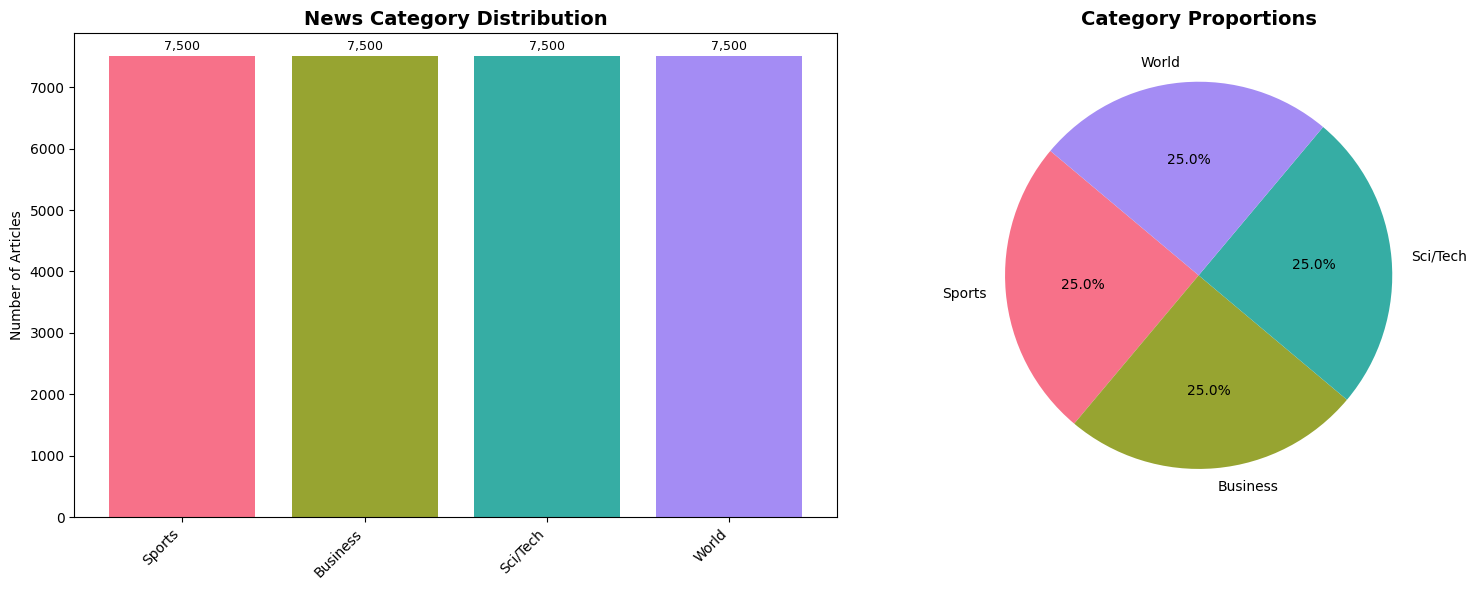
\includegraphics[width=0.82\textwidth,height=0.42\textheight,keepaspectratio]{figs/e9_9_0.png}\caption{News Category Distribution}\end{figure}
\Needspace{14\baselineskip}\paragraph{Output 5: Text Length Analysis}\mbox{}\\[-1ex]
\begin{Verbatim}[commandchars=\\\{\},breaklines=true,breakanywhere=true,fontsize=\scriptsize,frame=leftline,framesep=2mm,rulecolor=\color{gray}]
 Word Count Statistics:
           count  mean   std   min   25%   50%   75%    max
category
Business  7500.0  37.6   8.1   8.0  32.0  37.0  42.0  126.0
Sci/Tech  7500.0  37.1  12.1   8.0  30.0  36.0  42.0  177.0
Sports    7500.0  37.8   8.7   8.0  32.0  37.0  43.0  103.0
World     7500.0  38.9  10.3  13.0  33.0  39.0  44.0  134.0
\end{Verbatim}
\begin{figure}[H]\centering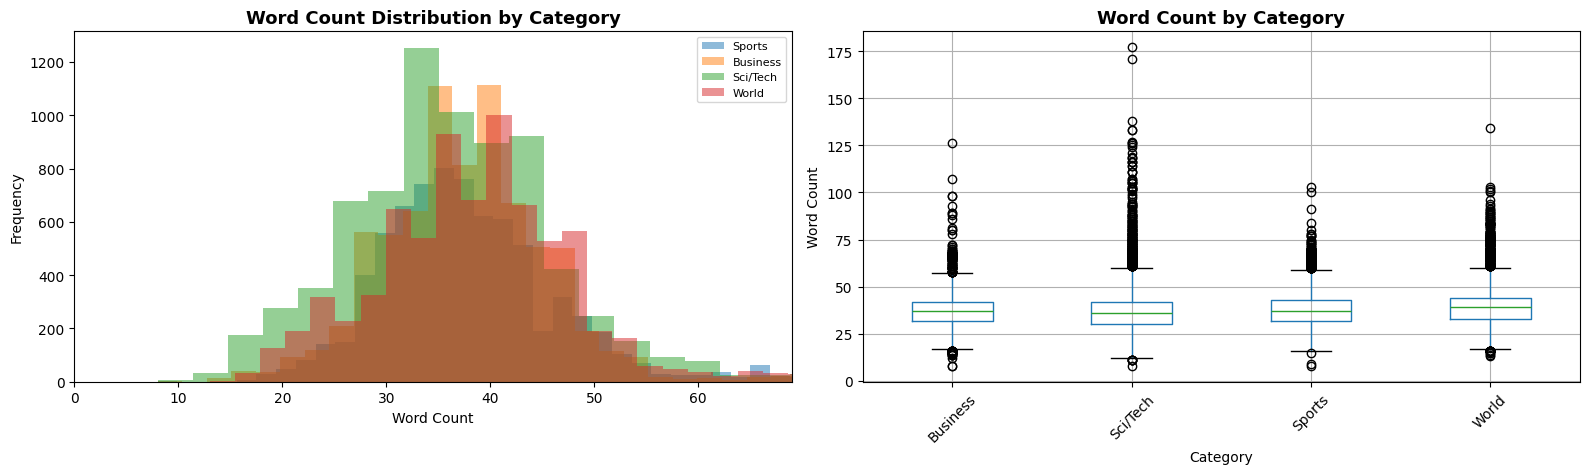
\includegraphics[width=0.82\textwidth,height=0.42\textheight,keepaspectratio]{figs/e9_10_0.png}\caption{Word Count Distribution by Category}\end{figure}
\Needspace{14\baselineskip}\paragraph{Output 6: WordCloud Visualization}\mbox{}\\[-1ex]
\begin{figure}[H]\centering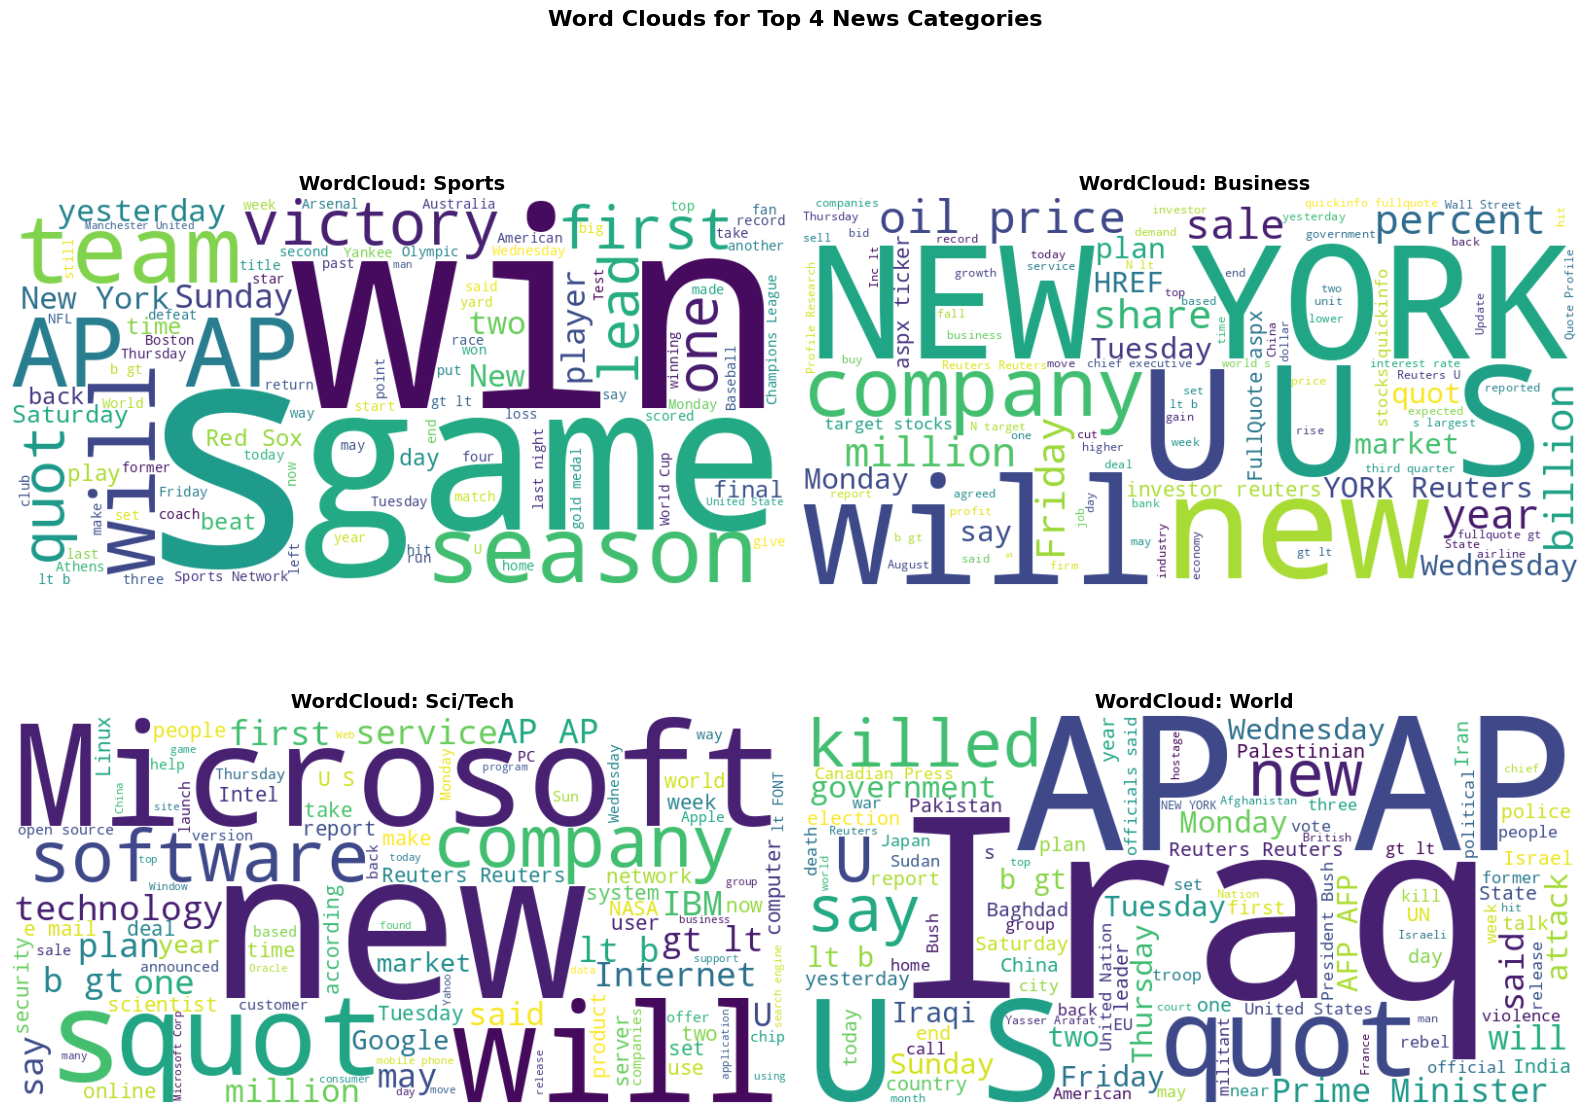
\includegraphics[width=0.82\textwidth,height=0.42\textheight,keepaspectratio]{figs/e9_11_0.png}\caption{Word Clouds for Top 4 News Categories}\end{figure}
\Needspace{14\baselineskip}\paragraph{Output 7: Text Preprocessing Pipeline}\mbox{}\\[-1ex]
\begin{Verbatim}[commandchars=\\\{\},breaklines=true,breakanywhere=true,fontsize=\scriptsize,frame=leftline,framesep=2mm,rulecolor=\color{gray}]
 Cleaning text data...
   Removed 0 empty/very short rows

 Label Encoding:
   0: Business
   1: Sci/Tech
   2: Sports
   3: World

 Preprocessing complete! Dataset size: 30,000 samples
   Clean text sample: 'donald is fired up to carry form to detroit luke donald hailed yesterday s european masters victory ...'
\end{Verbatim}
\Needspace{14\baselineskip}\paragraph{Output 8: Stratified Train/Validation/Test Split}\mbox{}\\[-1ex]
\begin{Verbatim}[commandchars=\\\{\},breaklines=true,breakanywhere=true,fontsize=\scriptsize,frame=leftline,framesep=2mm,rulecolor=\color{gray}]
============================================================
DATASET SPLIT VERIFICATION
============================================================

 Total samples: 30,000
   Training:   24,000 (80.0%)
   Validation: 3,000 (10.0%)
   Test:       3,000 (10.0%)

 Class proportions are consistent across all 3 splits!
\end{Verbatim}
\begin{figure}[H]\centering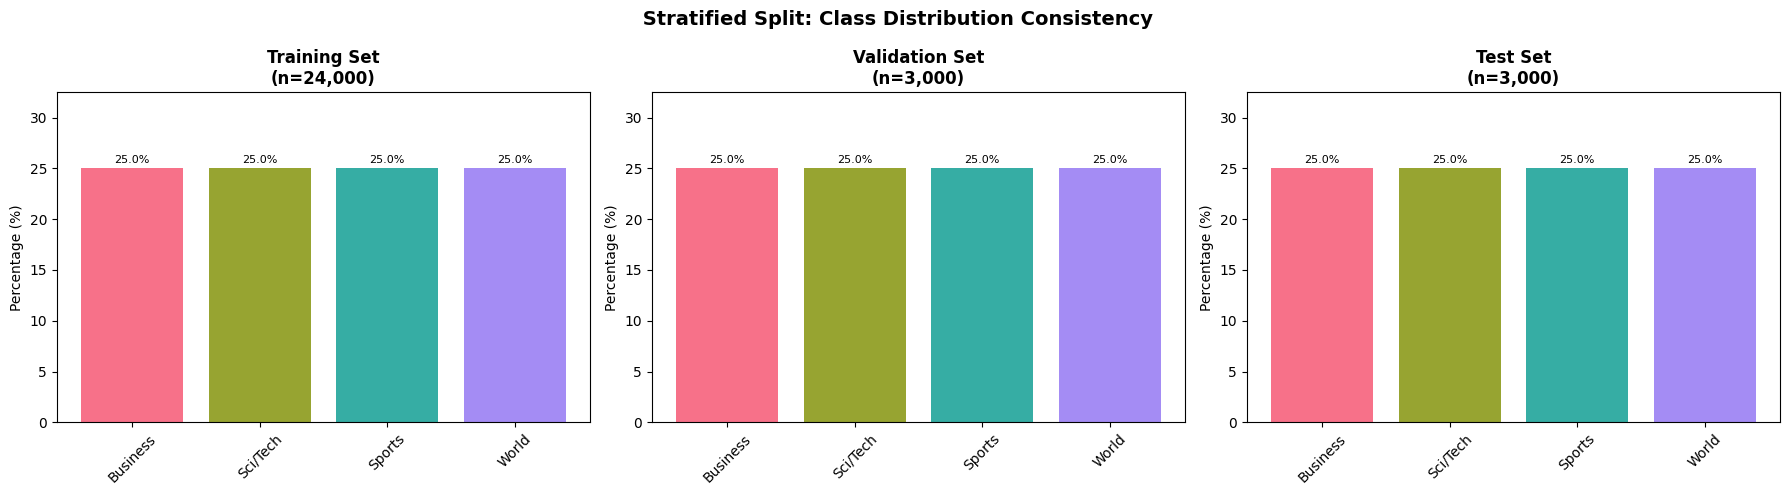
\includegraphics[width=0.82\textwidth,height=0.42\textheight,keepaspectratio]{figs/e9_15_0.png}\caption{ Stratified Split: Class Distribution Consistency}\end{figure}
\Needspace{14\baselineskip}\paragraph{Output 9: MODEL 1: TF-IDF + Linear SVC}\mbox{}\\[-1ex]
\begin{Verbatim}[commandchars=\\\{\},breaklines=true,breakanywhere=true,fontsize=\scriptsize,frame=leftline,framesep=2mm,rulecolor=\color{gray}]
============================================================
MODEL 1: TF-IDF + LinearSVC
============================================================
 Fitting TF-IDF vectorizer...
   Vocabulary size: 10,000
   Feature matrix shape: (24000, 10000)

 Training LinearSVC...
   Training completed in 4.13 seconds

 Validation Accuracy: 0.9023

 Test Results:
   Accuracy:  0.9137
   Macro F1:  0.9136
   Inference:  0.003 ms/sample

 Classification Report:
              precision    recall  f1-score   support

    Business       0.89      0.89      0.89       750
    Sci/Tech       0.88      0.89      0.89       750
      Sports       0.96      0.97      0.97       750
       World       0.93      0.90      0.91       750

    accuracy                           0.91      3000
   macro avg       0.91      0.91      0.91      3000
weighted avg       0.91      0.91      0.91      3000
\end{Verbatim}
\begin{figure}[H]\centering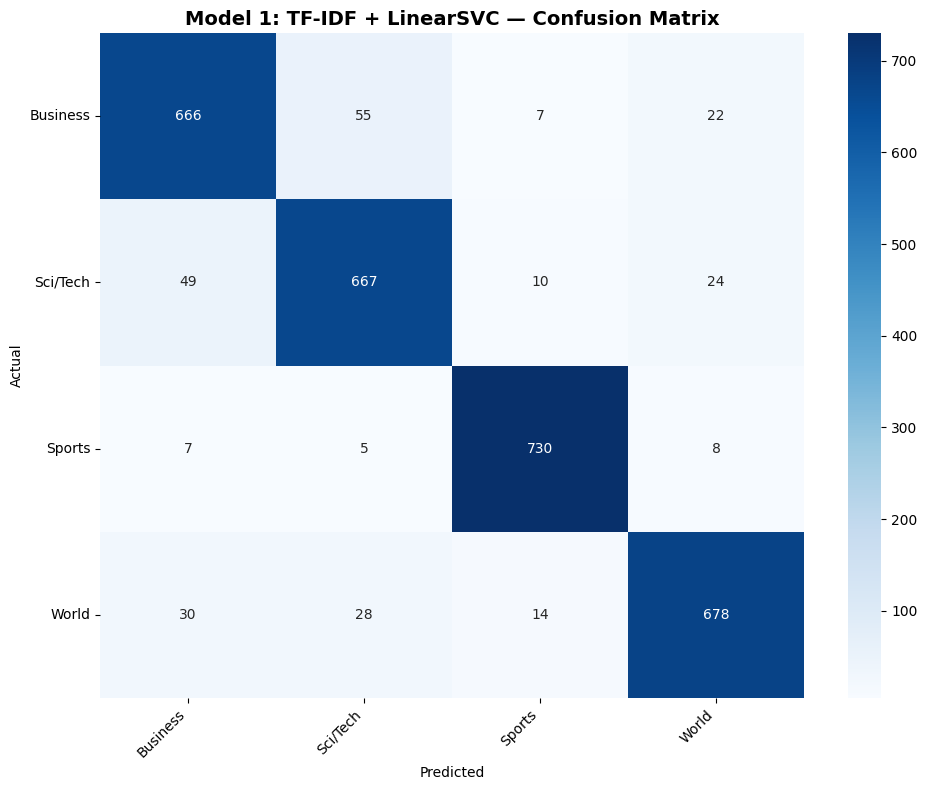
\includegraphics[width=0.82\textwidth,height=0.42\textheight,keepaspectratio]{figs/e9_17_0.png}\caption{Model 1: TF-IDF + LinearSVC — Confusion Matrix}\end{figure}
\Needspace{14\baselineskip}\paragraph{Output 10: MODEL 2: Bi-LSTM with Word Embeddings (TensorFlow/Keras)}\mbox{}\\[-1ex]
\begin{Verbatim}[commandchars=\\\{\},breaklines=true,breakanywhere=true,fontsize=\scriptsize,frame=leftline,framesep=2mm,rulecolor=\color{gray}]
============================================================
MODEL 2: Bidirectional LSTM
============================================================
 Building text vectorizer...
   Vocabulary size: 20000

 Building Bi-LSTM model...
Model: "sequential"
┏━━━━━━━━━━━━━━━━━━━━━━━━━━━━━━━━━┳━━━━━━━━━━━━━━━━━━━━━━━━┳━━━━━━━━━━━━━━━┓
┃ Layer (type)                    ┃ Output Shape           ┃       Param # ┃
┡━━━━━━━━━━━━━━━━━━━━━━━━━━━━━━━━━╇━━━━━━━━━━━━━━━━━━━━━━━━╇━━━━━━━━━━━━━━━┩
│ text_vectorization              │ (None, 150)            │             0 │
│ (TextVectorization)             │                        │               │
├─────────────────────────────────┼────────────────────────┼───────────────┤
│ embedding (Embedding)           │ (None, 150, 128)       │     2,560,000 │
├─────────────────────────────────┼────────────────────────┼───────────────┤
│ spatial_dropout1d               │ (None, 150, 128)       │             0 │
│ (SpatialDropout1D)              │                        │               │
├─────────────────────────────────┼────────────────────────┼───────────────┤
│ bidirectional (Bidirectional)   │ (None, 128)            │        98,816 │
├─────────────────────────────────┼────────────────────────┼───────────────┤
│ batch_normalization             │ (None, 128)            │           512 │
│ (BatchNormalization)            │                        │               │
├─────────────────────────────────┼────────────────────────┼───────────────┤
│ dense (Dense)                   │ (None, 64)             │         8,256 │
├─────────────────────────────────┼────────────────────────┼───────────────┤
│ dropout (Dropout)               │ (None, 64)             │             0 │
├─────────────────────────────────┼────────────────────────┼───────────────┤
│ dense_1 (Dense)                 │ (None, 4)              │           260 │
└─────────────────────────────────┴────────────────────────┴───────────────┘
 Total params: 2,667,844 (10.18 MB)
 Trainable params: 2,667,588 (10.18 MB)
 Non-trainable params: 256 (1.00 KB)

 Training Bi-LSTM...
Epoch 1/15
375/375 ━━━━━━━━━━━━━━━━━━━━ 35s 45ms/step - accuracy: 0.8215 - loss: 0.4969 - val_accuracy: 0.8873 - val_loss: 0.4674 - learning_rate: 0.0010
Epoch 2/15
375/375 ━━━━━━━━━━━━━━━━━━━━ 13s 35ms/step - accuracy: 0.9449 - loss: 0.1737 - val_accuracy: 0.8610 - val_loss: 0.4952 - learning_rate: 0.0010
Epoch 3/15
375/375 ━━━━━━━━━━━━━━━━━━━━ 22s 39ms/step - accuracy: 0.9743 - loss: 0.0808 - val_accuracy: 0.8427 - val_loss: 0.6979 - learning_rate: 0.0010
Epoch 4/15
375/375 ━━━━━━━━━━━━━━━━━━━━ 14s 37ms/step - accuracy: 0.9848 - loss: 0.0477 - val_accuracy: 0.8653 - val_loss: 0.6770 - learning_rate: 0.0010
Epoch 4: early stopping
Restoring model weights from the end of the best epoch: 1.
... [output truncated for length]
\end{Verbatim}
\Needspace{14\baselineskip}\paragraph{Output 11: Learning Curves}\mbox{}\\[-1ex]
\begin{figure}[H]\centering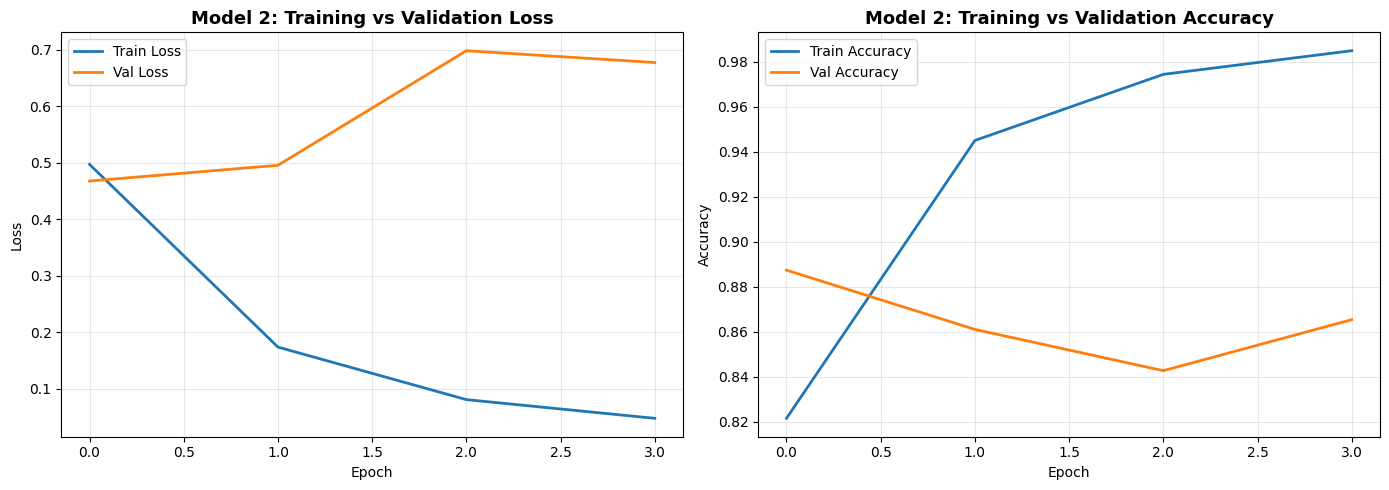
\includegraphics[width=0.82\textwidth,height=0.42\textheight,keepaspectratio]{figs/e9_20_0.png}\caption{Model 2: Training vs Validation Loss}\end{figure}
\Needspace{14\baselineskip}\paragraph{Output 12: Bi-LSTM Test Evaluation}\mbox{}\\[-1ex]
\begin{Verbatim}[commandchars=\\\{\},breaklines=true,breakanywhere=true,fontsize=\scriptsize,frame=leftline,framesep=2mm,rulecolor=\color{gray}]
 Test Results:
   Accuracy:  0.9073
   Macro F1:  0.9069
   Inference:  0.720 ms/sample

 Classification Report:
              precision    recall  f1-score   support

    Business       0.86      0.90      0.88       750
    Sci/Tech       0.92      0.84      0.88       750
      Sports       0.95      0.98      0.96       750
       World       0.90      0.91      0.91       750

    accuracy                           0.91      3000
   macro avg       0.91      0.91      0.91      3000
weighted avg       0.91      0.91      0.91      3000
\end{Verbatim}
\begin{figure}[H]\centering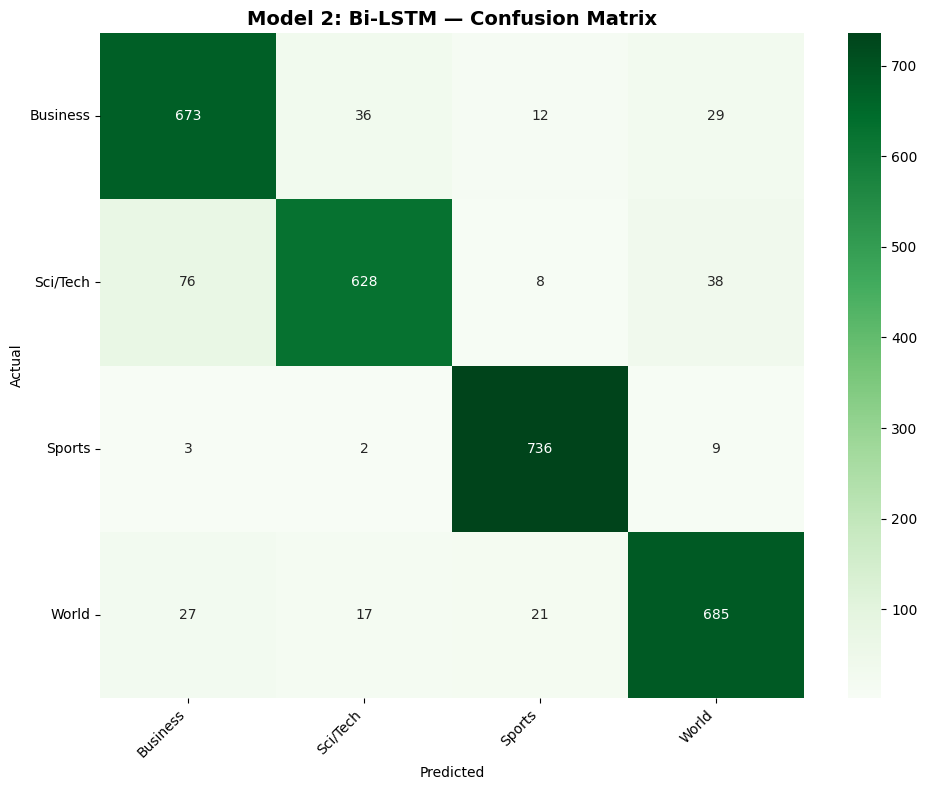
\includegraphics[width=0.82\textwidth,height=0.42\textheight,keepaspectratio]{figs/e9_21_0.png}\caption{Model 2: Bi-LSTM — Confusion Matrix}\end{figure}
\Needspace{14\baselineskip}\paragraph{Output 13: MODEL 3: Fine-tuned DistilBERT}\mbox{}\\[-1ex]
\begin{Verbatim}[commandchars=\\\{\},breaklines=true,breakanywhere=true,fontsize=\scriptsize,frame=leftline,framesep=2mm,rulecolor=\color{gray}]
============================================================
MODEL 3: DistilBERT (Fine-tuned Transformer)
============================================================
 Loading tokenizer: distilbert-base-uncased
   Tokenization complete
   Input IDs shape: torch.Size([24000, 128])
\end{Verbatim}
\Needspace{14\baselineskip}\paragraph{Output 14: PyTorch Dataset}\mbox{}\\[-1ex]
\begin{Verbatim}[commandchars=\\\{\},breaklines=true,breakanywhere=true,fontsize=\scriptsize,frame=leftline,framesep=2mm,rulecolor=\color{gray}]
   DataLoaders created
   Train batches: 750
   Val batches:   94
   Test batches:  94
\end{Verbatim}
\Needspace{14\baselineskip}\paragraph{Output 15: Load \& Fine-tune DistilBERT}\mbox{}\\[-1ex]
\begin{Verbatim}[commandchars=\\\{\},breaklines=true,breakanywhere=true,fontsize=\scriptsize,frame=leftline,framesep=2mm,rulecolor=\color{gray}]
 Loading distilbert-base-uncased for sequence classification...
Key                     | Status     |
pre_classifier.bias     | MISSING    |
pre_classifier.weight   | MISSING    |
classifier.weight       | MISSING    |
classifier.bias         | MISSING    |

Notes:
- MISSING:    those params were newly initialized because missing from the checkpoint. Consider training on your downstream task.
   Total parameters: 66,956,548
   Trainable parameters: 66,956,548

 Training DistilBERT for 3 epochs...
   Epoch 1/3 | Batch 50/750 | Loss: 0.4346
   Epoch 1/3 | Batch 100/750 | Loss: 0.5391
   Epoch 1/3 | Batch 150/750 | Loss: 0.3116
   Epoch 1/3 | Batch 200/750 | Loss: 0.3322
   Epoch 1/3 | Batch 250/750 | Loss: 0.4348
   Epoch 1/3 | Batch 300/750 | Loss: 0.3170
   Epoch 1/3 | Batch 350/750 | Loss: 0.1261
   Epoch 1/3 | Batch 400/750 | Loss: 0.4021
   Epoch 1/3 | Batch 450/750 | Loss: 0.4581
   Epoch 1/3 | Batch 500/750 | Loss: 0.4598
   Epoch 1/3 | Batch 550/750 | Loss: 0.1991
   Epoch 1/3 | Batch 600/750 | Loss: 0.1734
   Epoch 1/3 | Batch 650/750 | Loss: 0.1398
   Epoch 1/3 | Batch 700/750 | Loss: 0.1579
   Epoch 1/3 | Batch 750/750 | Loss: 0.0767

   Epoch 1/3: Train Loss=0.3197 | Train Acc=0.8990 | Val Loss=0.2435 | Val Acc=0.9200
   Epoch 2/3 | Batch 50/750 | Loss: 0.1031
   Epoch 2/3 | Batch 100/750 | Loss: 0.3808
   Epoch 2/3 | Batch 150/750 | Loss: 0.1251
   Epoch 2/3 | Batch 200/750 | Loss: 0.0736
   Epoch 2/3 | Batch 250/750 | Loss: 0.2143
   Epoch 2/3 | Batch 300/750 | Loss: 0.1601
   Epoch 2/3 | Batch 350/750 | Loss: 0.5322
   Epoch 2/3 | Batch 400/750 | Loss: 0.0781
   Epoch 2/3 | Batch 450/750 | Loss: 0.3446
   Epoch 2/3 | Batch 500/750 | Loss: 0.0734
   Epoch 2/3 | Batch 550/750 | Loss: 0.1428
   Epoch 2/3 | Batch 600/750 | Loss: 0.3543
   Epoch 2/3 | Batch 650/750 | Loss: 0.3275
   Epoch 2/3 | Batch 700/750 | Loss: 0.2306
   Epoch 2/3 | Batch 750/750 | Loss: 0.3143
... [output truncated for length]
\end{Verbatim}
\Needspace{14\baselineskip}\paragraph{Output 16: DistilBERT Test Evaluation}\mbox{}\\[-1ex]
\begin{Verbatim}[commandchars=\\\{\},breaklines=true,breakanywhere=true,fontsize=\scriptsize,frame=leftline,framesep=2mm,rulecolor=\color{gray}]
 Evaluating on Test Set...
   Accuracy:  0.9327
   Macro F1:  0.9327
   Inference:  3.349 ms/sample

 Classification Report:
              precision    recall  f1-score   support

    Business       0.91      0.89      0.90       750
    Sci/Tech       0.90      0.92      0.91       750
      Sports       0.99      0.98      0.98       750
       World       0.94      0.93      0.94       750

    accuracy                           0.93      3000
   macro avg       0.93      0.93      0.93      3000
weighted avg       0.93      0.93      0.93      3000
\end{Verbatim}
\begin{figure}[H]\centering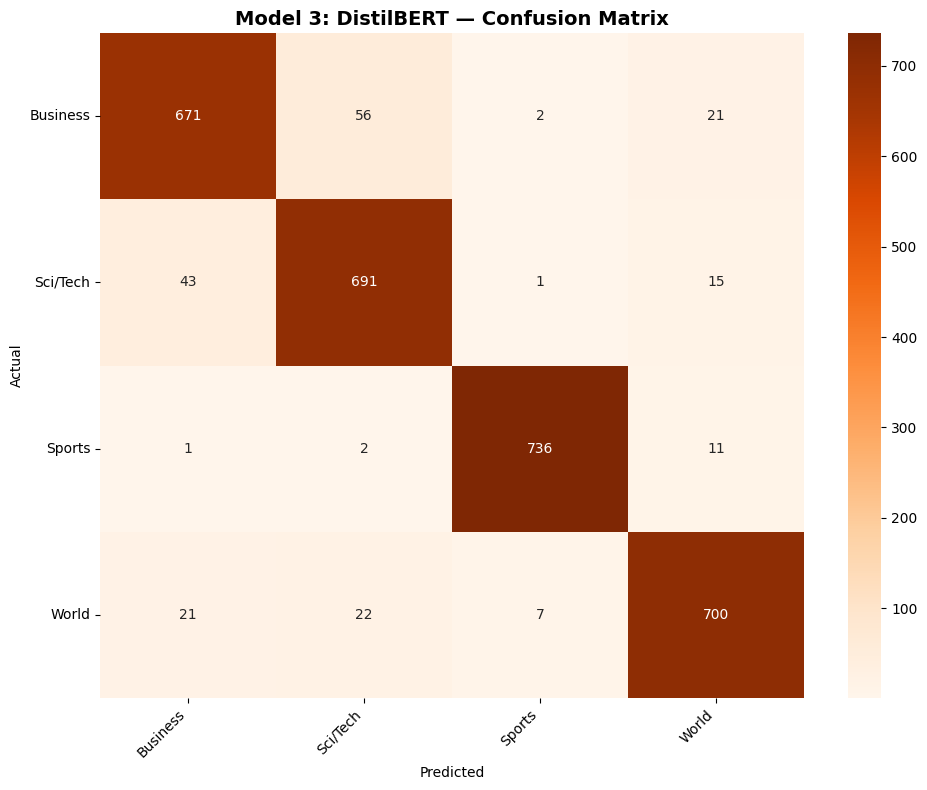
\includegraphics[width=0.82\textwidth,height=0.42\textheight,keepaspectratio]{figs/e9_26_0.png}\caption{Model 3: DistilBERT — Confusion Matrix}\end{figure}
\Needspace{14\baselineskip}\paragraph{Output 17: COMPREHENSIVE MODEL COMPARISON}\mbox{}\\[-1ex]
\begin{Verbatim}[commandchars=\\\{\},breaklines=true,breakanywhere=true,fontsize=\scriptsize,frame=leftline,framesep=2mm,rulecolor=\color{gray}]
============================================================
COMPREHENSIVE MODEL COMPARISON
============================================================

 Performance Comparison Table:
             Model      Paradigm  Test Accuracy  Macro Precision  Macro Recall  Macro F1  Training Time (s)  Inference (ms/sample)
TF-IDF + LinearSVC  Classical ML         0.9137           0.9136        0.9137    0.9136             4.1319                 0.0026
           Bi-LSTM Deep Learning         0.9073           0.9077        0.9073    0.9069            84.5880                 0.7196
        DistilBERT   Transformer         0.9327           0.9329        0.9327    0.9327           783.9358                 3.3488

 Best Model (by Macro F1): DistilBERT (0.9327)
 Comparison results saved to: /content/drive/MyDrive/NLP_Lab/Experiment-9/model_comparison_results.csv
\end{Verbatim}
\Needspace{14\baselineskip}\paragraph{Output 18: Comparison Visualizations}\mbox{}\\[-1ex]
\begin{figure}[H]\centering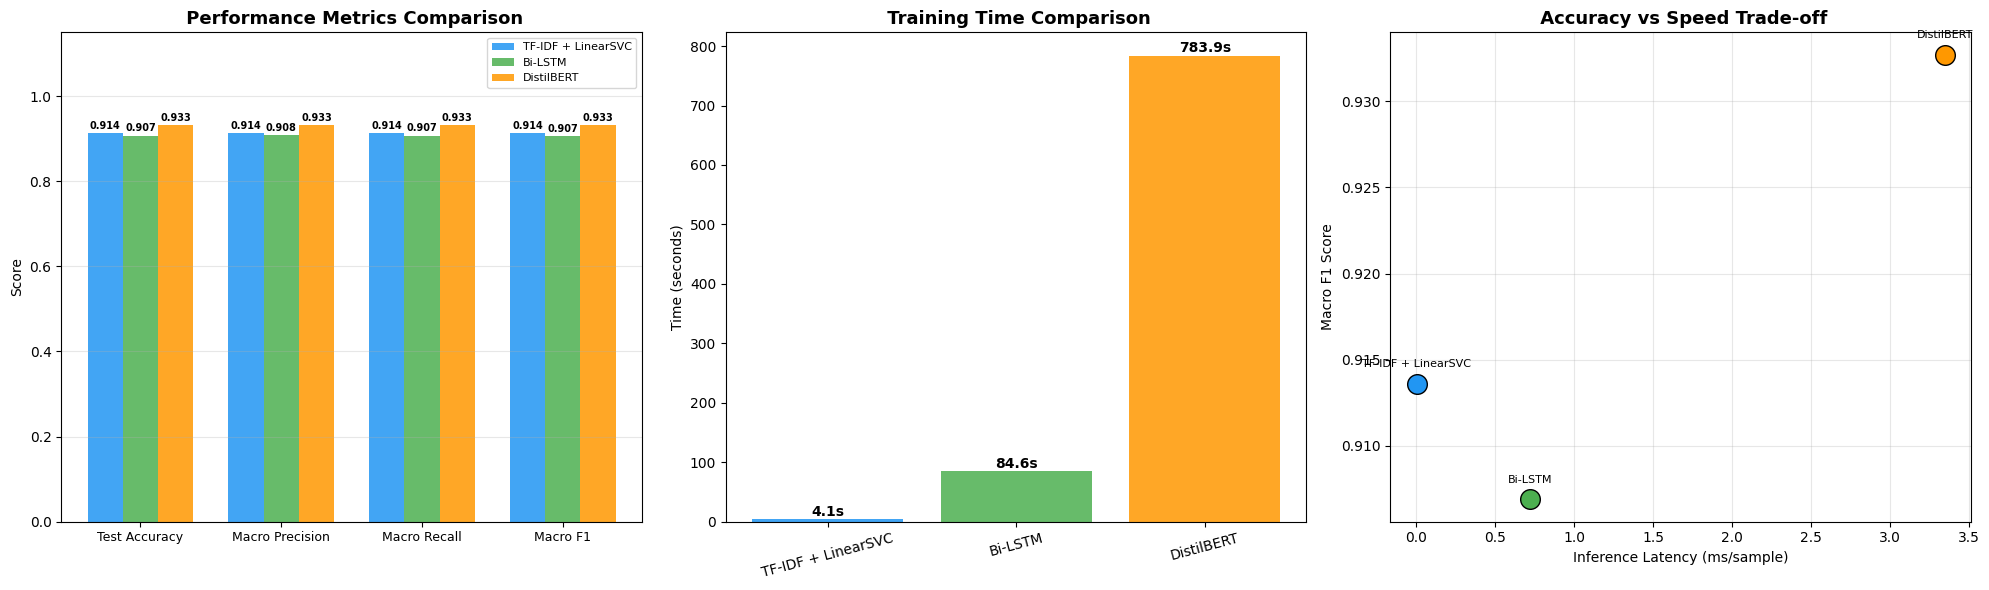
\includegraphics[width=0.82\textwidth,height=0.42\textheight,keepaspectratio]{figs/e9_29_0.png}\caption{ Performance Metrics Comparison}\end{figure}
\Needspace{14\baselineskip}\paragraph{Output 19: Side-by-Side Normalized Confusion Matrices}\mbox{}\\[-1ex]
\begin{figure}[H]\centering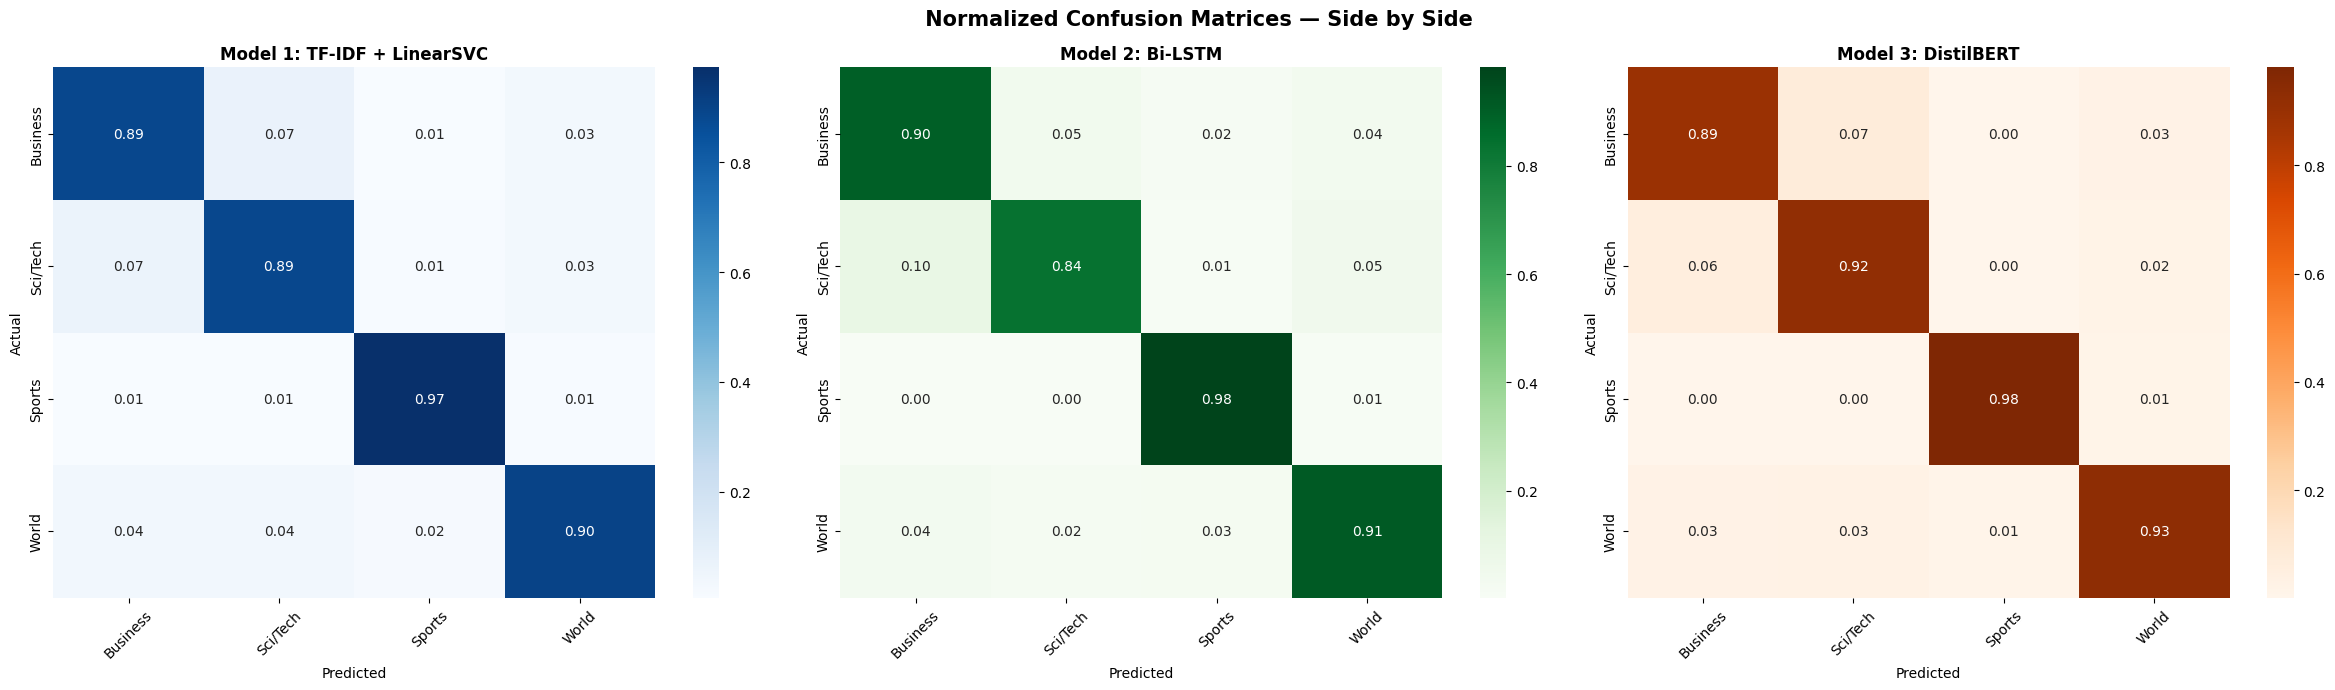
\includegraphics[width=0.82\textwidth,height=0.42\textheight,keepaspectratio]{figs/e9_30_0.png}\caption{ Normalized Confusion Matrices — Side by Side}\end{figure}
\Needspace{14\baselineskip}\paragraph{Output 20: Per-Class F1 Radar Chart}\mbox{}\\[-1ex]
\begin{figure}[H]\centering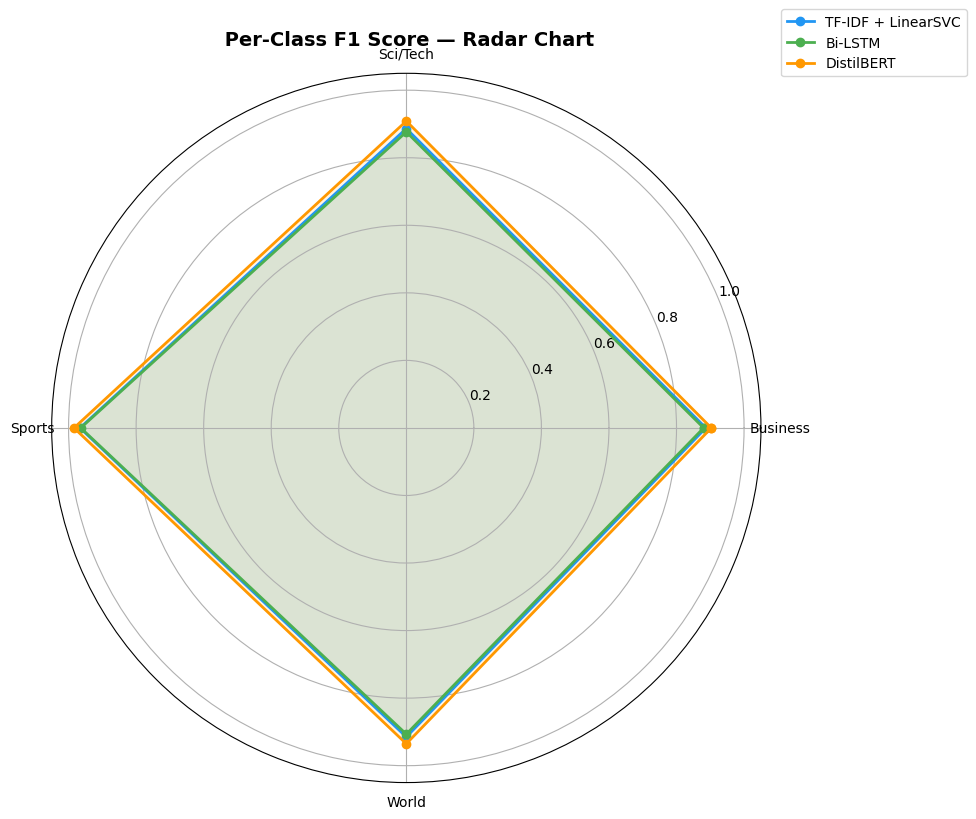
\includegraphics[width=0.82\textwidth,height=0.42\textheight,keepaspectratio]{figs/e9_31_0.png}\caption{ Per-Class F1 Score — Radar Chart}\end{figure}
\Needspace{14\baselineskip}\paragraph{Output 21: Error Analysis}\mbox{}\\[-1ex]
\begin{Verbatim}[commandchars=\\\{\},breaklines=true,breakanywhere=true,fontsize=\scriptsize,frame=leftline,framesep=2mm,rulecolor=\color{gray}]
============================================================
QUALITATIVE ERROR ANALYSIS
============================================================

 Models disagree on 317 / 3000 test samples (10.6%)

 Sample Predictions Where Models Disagree:

#    True Label      TF-IDF+SVC      Bi-LSTM         DistilBERT      Text Preview
-------------------------------------------------------------------------------------------------------------------
1    World           Yes World        No Business     No Business     war funding request may hit billion washington ...
2    Business        No Sci/Tech     Yes Business     No Sci/Tech     diesels hybrids fated to wed two leading techno...
3    Sci/Tech        No World        No World        Yes Sci/Tech     new media battle for bafta awards the bbc leads...
4    Business        No Sci/Tech     No Sci/Tech     Yes Business     stress free shopping with a seasoned pro bring ...
5    Business        Yes Business     Yes Business     No Sci/Tech     europe starts new microsoft probe the european ...
6    Sci/Tech        No Business     No Business     Yes Sci/Tech     former ca chief indicted company reaches accord...
7    Sports          Yes Sports       No World        Yes Sports       debut at lambeau growing up in brandon israel i...
8    Sci/Tech        Yes Sci/Tech     No Business     Yes Sci/Tech     at amp t uses its long past to promote its near...
9    Business        No Sports       No Sports       Yes Business     the midas touch with spin on it hen donald j tr...
10   Sci/Tech        Yes Sci/Tech     No Business     Yes Sci/Tech     ibm s blue gene to topple japanese supercompute...

 Error Rate by Category:
Category           TF-IDF+SVC      Bi-LSTM         DistilBERT
-----------------------------------------------------------------
Business               11.2%          10.3%          10.5%
Sci/Tech               11.1%          16.3%           7.9%
Sports                  2.7%           1.9%           1.9%
World                   9.6%           8.7%           6.7%
\end{Verbatim}
\Needspace{14\baselineskip}\paragraph{Output 22: Live Inference Function}\mbox{}\\[-1ex]
\begin{Verbatim}[commandchars=\\\{\},breaklines=true,breakanywhere=true,fontsize=\scriptsize,frame=leftline,framesep=2mm,rulecolor=\color{gray}]
 LIVE INFERENCE DEMO

============================================================
 Input: Apple reports record quarterly revenue driven by iPhone sales
============================================================

Model                     Prediction         Confidence
-------------------------------------------------------
TF-IDF + LinearSVC        Business               61.7%
Bi-LSTM                   Business               49.4%
DistilBERT                Sci/Tech               82.3%

 Consensus (2/3 models agree): Business

============================================================
 Input: UN Security Council holds emergency summit on international peace treaty
============================================================

Model                     Prediction         Confidence
-------------------------------------------------------
TF-IDF + LinearSVC        World                  95.8%
Bi-LSTM                   World                  88.1%
DistilBERT                World                  99.7%

 Consensus (3/3 models agree): World

============================================================
 Input: Manchester United signs new striker in record transfer deal
============================================================

Model                     Prediction         Confidence
-------------------------------------------------------
TF-IDF + LinearSVC        Sports                 97.9%
Bi-LSTM                   Sports                 83.0%
DistilBERT                Sports                 99.3%

 Consensus (3/3 models agree): Sports
\end{Verbatim}
\textbf{Observations.}

\begin{longtable}[]{@{}
  >{\raggedright\arraybackslash}p{(\columnwidth - 8\tabcolsep) * \real{0.2000}}
  >{\raggedright\arraybackslash}p{(\columnwidth - 8\tabcolsep) * \real{0.2000}}
  >{\raggedright\arraybackslash}p{(\columnwidth - 8\tabcolsep) * \real{0.2000}}
  >{\raggedright\arraybackslash}p{(\columnwidth - 8\tabcolsep) * \real{0.2000}}
  >{\raggedright\arraybackslash}p{(\columnwidth - 8\tabcolsep) * \real{0.2000}}@{}}
\toprule\noalign{}
\begin{minipage}[b]{\linewidth}\raggedright
Model
\end{minipage} & \begin{minipage}[b]{\linewidth}\raggedright
Accuracy
\end{minipage} & \begin{minipage}[b]{\linewidth}\raggedright
Macro F1
\end{minipage} & \begin{minipage}[b]{\linewidth}\raggedright
Training time (s)
\end{minipage} & \begin{minipage}[b]{\linewidth}\raggedright
Inference (ms/sample)
\end{minipage} \\
\midrule\noalign{}
\endhead
\bottomrule\noalign{}
\endlastfoot
TF-IDF + LinearSVC & 0.9137 & 0.9136 & 4.1 & 0.003 \\
Bi-LSTM & 0.9073 & 0.9069 & 84.6 & 0.720 \\
DistilBERT & 0.9327 & 0.9327 & 783.9 & 3.349 \\
\end{longtable}

\begin{itemize}
\tightlist
\item
  DistilBERT is the most accurate model, about two points above the linear baseline, but it takes roughly 190 times longer to train and about 1,000 times longer per prediction than LinearSVC.
\item
  The Bi-LSTM did not beat the TF-IDF baseline on this subset, and it is slower to train.
\item
  In all three models, Sports is classified best (F1 about 0.96 to 0.98) and Business and Sci/Tech are the most confused pair, as their vocabularies overlap.
\end{itemize}


\section{Conclusion}
\hypertarget{key-findings}{%
\subsection{Key Findings}\label{key-findings}}

\begin{enumerate}
\def\labelenumi{\arabic{enumi}.}
\tightlist
\item
  \textbf{TF-IDF + LinearSVC} provides a strong baseline with extremely fast training and inference --- ideal for production systems where speed matters.
\item
  \textbf{Bi-LSTM} captures sequential patterns and word order, offering a good balance between accuracy and complexity.
\item
  \textbf{DistilBERT} achieves the best performance by leveraging pretrained language understanding from massive corpora, though it comes with higher computational cost.
\end{enumerate}

\hypertarget{model-recommendation}{%
\subsection{Model Recommendation}\label{model-recommendation}}

Use Case \textbar{} Recommended Model \textbar{}\\

\chapter{Experiment 10: Low-Resource Neural Machine Translation (English to Hindi)}
\section{Abstract}
Neural Machine Translation (NMT) for low-resource languages presents severe optimization challenges due to parallel corpus scarcity, high out-of-vocabulary rates, complex morphological structures, and diverse non-Latin scripts. This experiment provides an end-to-end comparative study of neural translation paradigms on a simulated low-resource \textbf{English → Hindi} translation task using a 10,000-sentence subset of the \textbf{IIT Bombay English-Hindi Parallel Corpus}. Three distinct architectural paradigms are designed, trained, and benchmarked: (1) an \textbf{RNN-based Seq2Seq model with Bahdanau Additive Attention} (bidirectional GRU encoder, attention mechanism, and GRU decoder with teacher forcing); (2) a \textbf{Transformer model implemented from scratch} featuring sinusoidal positional encodings, multi-head self-attention, and position-wise feed-forward networks; and (3) a \textbf{Pretrained Multilingual Transfer Model (MarianMT / OPUS-MT \texttt{Helsinki-NLP/opus-mt-en-hi})} fine-tuned on the low-resource parallel data. All models are rigorously evaluated using standardized automatic translation metrics: \textbf{BLEU} (sacrebleu), \textbf{chrF} (character n-gram F-score), \textbf{TER} (Translation Edit Rate), and \textbf{ROUGE-L}, alongside training loss convergence dynamics, inference latency, and qualitative error analysis across 15 representative test sentences. The empirical findings reveal that while from-scratch models struggle under severe data scarcity, pretrained multilingual models leverage cross-lingual representations to drastically outperform scratch architectures in fluency, vocabulary coverage, and syntactic fidelity.

\section{Aim}
To build, train, and evaluate three neural machine translation (NMT) architectures on a low-resource English--Hindi translation task, comparing their translation quality (BLEU, chrF, TER, ROUGE-L), computational efficiency (training time, inference time), and suitability for low-resource scenarios.

\textbf{Dataset Reference:} \href{https://www2.statmt.org/wmt26/indic-mt-task.html}{WMT 2026 Shared Task on Low-Resource Indic Language Translation}

\hypertarget{language-pair-selection-english-hindi}{%
\subsection{Language Pair Selection: English → Hindi}\label{language-pair-selection-english-hindi}}

The WMT 2026 Indic MT Task covers ten English--Indic language pairs including Assamese, Mizo, Khasi, Manipuri, Bodo, Kokborok, and others. For this experiment, we select \textbf{English → Hindi} and simulate a low-resource setting by using a small subset (configurable, default 10,000 pairs) of the IIT Bombay English-Hindi Parallel Corpus.

\textbf{Why this choice?}
1. \textbf{Practical availability:} The IIT Bombay corpus is freely available on Hugging Face (\texttt{cfilt/iitb-english-hindi}), ensuring reproducibility.
2. \textbf{Pretrained model access:} A pretrained MarianMT model (\texttt{Helsinki-NLP/opus-mt-en-hi}) exists for this pair, enabling meaningful comparison of transfer learning vs.~training from scratch.
3. \textbf{Low-resource simulation:} By restricting training data to 10K pairs, we faithfully simulate the data scarcity challenges faced by truly low-resource languages like Mizo or Khasi.
4. \textbf{Script diversity:} Hindi uses Devanagari script, presenting real challenges for character-level and subword tokenization --- similar to other Indic scripts.

\section{Description and Theoretical Background}
\hypertarget{neural-machine-translation-nmt}{%
\subsection{Neural Machine Translation (NMT)}\label{neural-machine-translation-nmt}}

Neural Machine Translation uses deep neural networks to learn the mapping from a source language to a target language in an end-to-end fashion. Unlike traditional statistical MT, NMT models learn distributed representations of words and sentences, enabling better handling of long-range dependencies and morphological variations.

\hypertarget{low-resource-translation-challenges}{%
\subsection{Low-Resource Translation Challenges}\label{low-resource-translation-challenges}}

Low-resource languages suffer from:
- \textbf{Limited parallel data} for training supervised models
- \textbf{Morphological complexity} that requires more data to learn patterns
- \textbf{Script diversity} making tokenization non-trivial
- \textbf{Lack of pretrained resources} such as embeddings and language models

\hypertarget{model-architectures}{%
\subsection{Model Architectures}\label{model-architectures}}

\hypertarget{model-1-rnn-based-seq2seq-with-attention}{%
\subsubsection{Model 1: RNN-based Seq2Seq with Attention}\label{model-1-rnn-based-seq2seq-with-attention}}

The encoder-decoder framework with attention (Bahdanau et al., 2015) uses:
- \textbf{Encoder:} A bidirectional GRU processes the source sentence into context vectors
- \textbf{Attention Mechanism:} Computes a weighted sum of encoder outputs, allowing the decoder to focus on relevant parts of the source at each decoding step
- \textbf{Decoder:} A GRU generates the target sequence one token at a time, conditioned on the attention context and previous token

\hypertarget{model-2-transformer}{%
\subsubsection{Model 2: Transformer}\label{model-2-transformer}}

The Transformer (Vaswani et al., 2017) replaces recurrence with:
- \textbf{Multi-Head Self-Attention:} Captures dependencies between all positions simultaneously
- \textbf{Positional Encoding:} Injects sequence order information using sinusoidal functions
- \textbf{Feed-Forward Layers:} Apply non-linear transformations at each position
- \textbf{Encoder-Decoder Architecture:} The decoder attends to both its own previous outputs and the encoder output

\hypertarget{model-3-pretrained-multilingual-model-marianmt}{%
\subsubsection{Model 3: Pretrained Multilingual Model (MarianMT)}\label{model-3-pretrained-multilingual-model-marianmt}}

Pretrained models leverage transfer learning:
- Trained on large multilingual corpora (OPUS), they learn cross-lingual representations
- Fine-tuning on a small target dataset adapts the model to the specific language pair
- This approach is especially powerful for low-resource languages, as the model has already learned general translation patterns from high-resource pairs

\hypertarget{evaluation-metrics}{%
\subsection{Evaluation Metrics}\label{evaluation-metrics}}

\begin{longtable}[]{@{}
  >{\raggedright\arraybackslash}p{(\columnwidth - 2\tabcolsep) * \real{0.3810}}
  >{\raggedright\arraybackslash}p{(\columnwidth - 2\tabcolsep) * \real{0.6190}}@{}}
\toprule\noalign{}
\begin{minipage}[b]{\linewidth}\raggedright
Metric
\end{minipage} & \begin{minipage}[b]{\linewidth}\raggedright
Description
\end{minipage} \\
\midrule\noalign{}
\endhead
\bottomrule\noalign{}
\endlastfoot
\textbf{BLEU} & Measures n-gram overlap between generated and reference translations (higher is better) \\
\textbf{chrF} & Character n-gram F-score, more robust for morphologically rich languages (higher is better) \\
\textbf{TER} & Translation Edit Rate --- minimum edits to transform output into reference (lower is better) \\
\textbf{ROUGE-L} & Longest Common Subsequence based metric measuring sequence similarity (higher is better) \\
\end{longtable}

\section{Data Understanding and Preprocessing}
The data is a 10,000-pair subset of the IIT Bombay English-Hindi parallel corpus (full corpus size 1,659,083 pairs) used to simulate a low-resource setting. After normalisation and filtering, the data is split into \textbf{5,383 training, 672 validation and 672 test} sentence pairs.

We load the \textbf{IIT Bombay English-Hindi Parallel Corpus} from Hugging Face. This corpus was developed by CFILT at IIT Bombay and is widely used in WMT shared tasks for English--Hindi translation benchmarking.

If the dataset cannot be downloaded (e.g., no internet), a small fallback dataset is used for demonstration.

Steps:
1. Remove duplicate sentence pairs
2. Remove empty or whitespace-only sentences
3. Basic text normalization (strip, lowercase for English)
4. Filter by sentence length
5. Split into train, validation, and test sets

\hypertarget{for-models-1-2-seq2seq-and-transformer}{%
\subsection{For Models 1 \& 2 (Seq2Seq and Transformer)}\label{for-models-1-2-seq2seq-and-transformer}}

We build word-level vocabularies from the training data with special tokens:
- \texttt{\textless{}PAD\textgreater{}} (0): Padding token
- \texttt{\textless{}SOS\textgreater{}} (1): Start of sentence
- \texttt{\textless{}EOS\textgreater{}} (2): End of sentence
- \texttt{\textless{}UNK\textgreater{}} (3): Unknown token

\hypertarget{for-model-3-marianmt}{%
\subsection{For Model 3 (MarianMT)}\label{for-model-3-marianmt}}

The pretrained model uses its own SentencePiece tokenizer, which is loaded separately.

\section{Methodology}
\hypertarget{model-1-seq2seq-with-attention}{%
\subsection{Model 1 -- Seq2Seq with Attention}\label{model-1-seq2seq-with-attention}}

\hypertarget{architecture}{%
\subsubsection{Architecture}\label{architecture}}

\begin{itemize}
\tightlist
\item
  \textbf{Encoder:} Bidirectional GRU that processes the source sentence and produces hidden states
\item
  \textbf{Bahdanau Attention:} Learns to align and weight encoder outputs for each decoder step
\item
  \textbf{Decoder:} GRU that generates one target token at a time, using the attention context
\end{itemize}

\hypertarget{key-components}{%
\subsubsection{Key Components}\label{key-components}}

\begin{enumerate}
\def\labelenumi{\arabic{enumi}.}
\tightlist
\item
  The \textbf{bidirectional encoder} reads the source in both directions, capturing left and right context
\item
  The \textbf{attention mechanism} computes alignment scores between the decoder state and all encoder states
\item
  \textbf{Teacher forcing} is used during training: with some probability, the decoder receives the true previous token instead of its own prediction
\end{enumerate}

\hypertarget{model-2-transformer}{%
\subsection{Model 2 -- Transformer}\label{model-2-transformer}}

\hypertarget{architecture-1}{%
\subsubsection{Architecture}\label{architecture-1}}

\begin{itemize}
\tightlist
\item
  \textbf{Positional Encoding:} Sinusoidal functions inject position information into embeddings
\item
  \textbf{Multi-Head Self-Attention:} Allows the model to jointly attend to information from different representation subspaces
\item
  \textbf{Encoder-Decoder Architecture:} Uses PyTorch's \texttt{nn.Transformer} with customizable layers and dimensions
\item
  \textbf{Causal Masking:} Prevents the decoder from attending to future positions during training
\end{itemize}

\hypertarget{key-advantages}{%
\subsubsection{Key Advantages}\label{key-advantages}}

\begin{itemize}
\tightlist
\item
  Parallelizable computation (no sequential recurrence)
\item
  Better at capturing long-range dependencies
\item
  Standard architecture in modern NMT systems
\end{itemize}

\hypertarget{model-3-pretrained-multilingual-model}{%
\subsection{Model 3 -- Pretrained Multilingual Model}\label{model-3-pretrained-multilingual-model}}

\hypertarget{about-marianmt}{%
\subsubsection{About MarianMT}\label{about-marianmt}}

MarianMT is an efficient neural machine translation framework. The \texttt{Helsinki-NLP/opus-mt-en-hi} model was pretrained on the OPUS parallel corpus collection, which includes millions of English-Hindi sentence pairs from diverse sources.

\hypertarget{transfer-learning-advantage}{%
\subsubsection{Transfer Learning Advantage}\label{transfer-learning-advantage}}

For low-resource translation, pretrained models offer significant advantages:
1. \textbf{Knowledge transfer:} The model has already learned general translation patterns, grammar structures, and vocabulary mappings from large-scale data
2. \textbf{Faster convergence:} Fine-tuning requires fewer epochs and less data than training from scratch
3. \textbf{Better generalization:} Pretrained representations help the model handle unseen words and sentence structures
4. \textbf{Subword tokenization:} SentencePiece tokenization handles out-of-vocabulary words gracefully by breaking them into subword units

\begin{quote}
\textbf{Note:} If the pretrained model cannot be downloaded, the notebook will skip Model 3 fine-tuning and use the model in zero-shot mode for evaluation.
\end{quote}

\hypertarget{model-training}{%
\subsection{Model Training}\label{model-training}}

\hypertarget{training-strategy}{%
\subsubsection{Training Strategy}\label{training-strategy}}

\begin{itemize}
\tightlist
\item
  \textbf{Models 1 \& 2:} Custom PyTorch training loop with early stopping based on validation loss
\item
  \textbf{Model 3:} HuggingFace \texttt{Seq2SeqTrainer} with early stopping callback
\item
  \textbf{GPU/CPU:} Automatically uses GPU if available
\item
  Training time is recorded for each model
\end{itemize}

\section{Evaluation and Metrics}
\hypertarget{evaluation-metrics}{%
\subsection{Evaluation Metrics}\label{evaluation-metrics}}

\begin{longtable}[]{@{}
  >{\raggedright\arraybackslash}p{(\columnwidth - 4\tabcolsep) * \real{0.2424}}
  >{\raggedright\arraybackslash}p{(\columnwidth - 4\tabcolsep) * \real{0.2727}}
  >{\raggedright\arraybackslash}p{(\columnwidth - 4\tabcolsep) * \real{0.4848}}@{}}
\toprule\noalign{}
\begin{minipage}[b]{\linewidth}\raggedright
Metric
\end{minipage} & \begin{minipage}[b]{\linewidth}\raggedright
Library
\end{minipage} & \begin{minipage}[b]{\linewidth}\raggedright
Interpretation
\end{minipage} \\
\midrule\noalign{}
\endhead
\bottomrule\noalign{}
\endlastfoot
\textbf{BLEU} & sacrebleu & Measures n-gram precision between hypothesis and reference. Score 0--100, higher is better. \\
\textbf{chrF} & sacrebleu & Character n-gram F-score. More robust for morphologically rich languages. Score 0--100, higher is better. \\
\textbf{TER} & sacrebleu & Translation Edit Rate --- the number of edits (insertions, deletions, substitutions, shifts) needed to match the reference, normalized by reference length. Lower is better. \\
\textbf{ROUGE-L} & rouge-score & Measures the longest common subsequence (LCS) between hypothesis and reference. Score 0--1, higher is better. \\
\textbf{Inference Time} & time & Wall-clock time to translate the entire test set. Lower is better. \\
\textbf{Training Time} & time & Wall-clock time for the full training procedure. Lower is better. \\
\end{longtable}

\section{Description of the Implemented Code}
\hypertarget{end-to-end-pipeline-architecture}{%
\subsection{End-to-End Pipeline Architecture}\label{end-to-end-pipeline-architecture}}

\begin{Verbatim}[breaklines=true,breakanywhere=true,fontsize=\scriptsize,frame=leftline,framesep=2mm]
┌──────────────────────────────────────────────────────────┐
│ Parallel Corpus: IIT Bombay English-Hindi (10,000 pairs) │
└────────────────────────────┬─────────────────────────────┘
                             │
                             ▼
┌──────────────────────────────────────────────────────────┐
│ Stage 1: Setup, Package Installation & Hardware Init     │
│ • Install PyTorch, Transformers, Datasets, SacreBLEU     │
│ • Set fixed seeds (SEED=42) & configure GPU/CUDA runtime │
└────────────────────────────┬─────────────────────────────┘
                             │
                             ▼
┌──────────────────────────────────────────────────────────┐
│ Stage 2: Data Ingestion, EDA & Preprocessing             │
│ • Stream 'cfilt/iitb-english-hindi' from Hugging Face    │
│ • Analyze sentence lengths, token frequencies & ratios   │
│ • Normalize Unicode, strip whitespace & deduplicate      │
│ • Split into Train (80%), Validation (10%), Test (10%)   │
└────────────────────────────┬─────────────────────────────┘
                             │
         ┌───────────────────┼───────────────────┐
         ▼                   ▼                   ▼
┌─────────────────┐ ┌─────────────────┐ ┌─────────────────┐
│ Stage 3:        │ │ Stage 4:        │ │ Stage 5:        │
│ Model 1: Seq2Seq│ │ Model 2: Scratch│ │ Model 3: Pre-   │
│ + Attention     │ │ Transformer     │ │ trained MarianMT│
│ • Word-level    │ │ • Word-level    │ │ • Subword       │
│   Vocabulary    │ │   Vocabulary    │ │   SentencePiece │
│   (min_freq=2)  │ │   (min_freq=2)  │ │   Tokenizer     │
│ • Bi-GRU Encoder│ │ • Sinusoidal    │ │ • Helsinki-NLP/ │
│ • Bahdanau      │ │   Positional Enc│ │   opus-mt-en-hi │
│   Additive Attn │ │ • Multi-Head    │ │ • Hugging Face  │
│ • GRU Decoder   │ │   Self-Attention│ │   Seq2SeqTrainer│
│ • Teacher       │ │ • PyTorch nn.   │ │   / AdamW fine- │
│   Forcing (0.5) │ │   Transformer   │ │   tuning loop   │
└────────┬────────┘ └────────┬────────┘ └────────┬────────┘
         └───────────────────┼───────────────────┘
                             │
                             ▼
┌──────────────────────────────────────────────────────────┐
│ Stage 6: Inference & Metric Evaluation                   │
│ • Greedy / Beam Search generation across test partition  │
│ • Automatic Metrics: BLEU, chrF, TER, ROUGE-L            │
│ • Computational Profiling: Epoch loss & inference speed │
└────────────────────────────┬─────────────────────────────┘
                             │
                             ▼
┌──────────────────────────────────────────────────────────┐
│ Stage 7: Visualization & Qualitative Diagnostic Analysis │
│ • Loss Convergence Plots (Seq2Seq vs Transf vs MarianMT) │
│ • Grouped Bar Charts for BLEU, chrF, TER, and ROUGE-L    │
│ • 15-Sample Qualitative Comparative Translation Table    │
└──────────────────────────────────────────────────────────┘
\end{Verbatim}

\begin{center}\rule{0.5\linewidth}{0.5pt}\end{center}

\hypertarget{code-description-by-module}{%
\subsection{Code Description by Module}\label{code-description-by-module}}

The notebook is systematically structured into modular stages:

\begin{enumerate}
\def\labelenumi{\arabic{enumi}.}
\tightlist
\item
  \textbf{Libraries, Dependencies \& Configuration (Cells 4--7)}:

  \begin{itemize}
  \tightlist
  \item
    Installs PyTorch, Transformers, Datasets, SentencePiece, SacreBLEU, and Accelerate.
  \item
    Imports core numerical, statistical, and neural network packages (\texttt{torch.nn}, \texttt{torch.optim}, \texttt{DataLoader}).
  \item
    Defines a global \texttt{CONFIG} dictionary setting random seeds (\texttt{42}), \texttt{MAX\_SAMPLES=10000}, \texttt{BATCH\_SIZE}, embedding dimensions, learning rates, and device management (\texttt{cuda} vs \texttt{cpu}).
  \end{itemize}
\item
  \textbf{Dataset Loading \& Exploratory Data Analysis (Cells 8--12)}:

  \begin{itemize}
  \tightlist
  \item
    Loads the \texttt{cfilt/iitb-english-hindi} parallel corpus from Hugging Face.
  \item
    Inspects dataset dimensions, displays parallel sentence pairs, and computes word-level length distributions and English-to-Hindi length ratios.
  \end{itemize}
\item
  \textbf{Data Preprocessing \& Splitting (Cells 13--15)}:

  \begin{itemize}
  \tightlist
  \item
    Normalizes Devanagari and Latin scripts via \texttt{unicodedata.normalize(\textquotesingle{}NFKC\textquotesingle{})} and regex cleaning.
  \item
    Removes duplicates, null records, and length outliers.
  \item
    Splits the clean parallel pairs into 80\% Train, 10\% Validation, and 10\% Test sets.
  \item
    Logs partition statistics ensuring zero cross-set leakage.
  \end{itemize}
\item
  \textbf{Tokenization \& Dataset Preparation (Cells 16--18)}:

  \begin{itemize}
  \tightlist
  \item
    Implements a custom \texttt{Vocabulary} class managing \texttt{\textless{}pad\textgreater{}}, \texttt{\textless{}sos\textgreater{}}, \texttt{\textless{}eos\textgreater{}}, and \texttt{\textless{}unk\textgreater{}} special tokens with frequency filtering (\texttt{min\_freq=2}).
  \item
    Constructs a custom PyTorch \texttt{TranslationDataset} with dynamic padding for batch execution.
  \end{itemize}
\item
  \textbf{Model 1: RNN Seq2Seq with Bahdanau Attention (Cells 19--20, 27--28)}:

  \begin{itemize}
  \tightlist
  \item
    Implements \texttt{Encoder} using a Bidirectional GRU to compute forward and backward annotation vectors.
  \item
    Implements \texttt{Attention} computing additive energy scores (\(e_{ij} = v^T \tanh(W_s s_{i-1} + W_h h_j)\)).
  \item
    Implements \texttt{Decoder} combining embedded previous tokens and attention context vectors into a GRU layer.
  \item
    Trains using Cross-Entropy loss with teacher forcing (ratio 0.5) over 10 epochs.
  \end{itemize}
\item
  \textbf{Model 2: Transformer from Scratch (Cells 21--22, 29)}:

  \begin{itemize}
  \tightlist
  \item
    Implements \texttt{PositionalEncoding} applying sinusoidal waveforms to inject sequence order.
  \item
    Configures PyTorch \texttt{nn.Transformer} (2 encoder layers, 2 decoder layers, 4 attention heads, \(d_{\text{model}}=128\), \(d_{\text{ff}}=256\)).
  \item
    Generates source padding masks and target causal triangular masks to prevent future token information leakage.
  \end{itemize}
\item
  \textbf{Model 3: Pretrained Multilingual MarianMT (Cells 23--25, 30)}:

  \begin{itemize}
  \tightlist
  \item
    Ingests \texttt{Helsinki-NLP/opus-mt-en-hi} subword tokenizer and Seq2Seq transformer model.
  \item
    Fine-tunes MarianMT using Hugging Face datasets and AdamW optimization on the low-resource parallel dataset.
  \end{itemize}
\item
  \textbf{Translation Inference \& Multi-Metric Evaluation (Cells 31--34)}:

  \begin{itemize}
  \tightlist
  \item
    Implements greedy and autoregressive decoding functions for all three models.
  \item
    Computes automated metrics across test hypotheses: \textbf{BLEU} (sacrebleu n-gram precision with brevity penalty), \textbf{chrF} (character n-gram F-score), \textbf{TER} (minimum edit rate), and \textbf{ROUGE-L} (longest common subsequence).
  \end{itemize}
\item
  \textbf{Visualizations, Comparison \& Qualitative Analysis (Cells 35--45)}:

  \begin{itemize}
  \tightlist
  \item
    Plots training and validation loss curves across all three models side-by-side.
  \item
    Renders grouped bar charts and radar comparison plots benchmarking BLEU, chrF, TER, and ROUGE-L.
  \item
    Formats a 15-sentence qualitative comparison table displaying Source, Reference, Seq2Seq, Transformer, and MarianMT outputs.
  \item
    Summarizes quantitative findings, low-resource trade-offs, and final conclusions.
  \end{itemize}
\end{enumerate}

\begin{center}\rule{0.5\linewidth}{0.5pt}\end{center}

\hypertarget{summary-of-operations-methods}{%
\subsection{Summary of Operations \& Methods}\label{summary-of-operations-methods}}

\begin{longtable}[]{@{}
  >{\raggedright\arraybackslash}p{(\columnwidth - 6\tabcolsep) * \real{0.2500}}
  >{\raggedright\arraybackslash}p{(\columnwidth - 6\tabcolsep) * \real{0.2500}}
  >{\raggedright\arraybackslash}p{(\columnwidth - 6\tabcolsep) * \real{0.2500}}
  >{\raggedright\arraybackslash}p{(\columnwidth - 6\tabcolsep) * \real{0.2500}}@{}}
\toprule\noalign{}
\begin{minipage}[b]{\linewidth}\raggedright
Module / Component
\end{minipage} & \begin{minipage}[b]{\linewidth}\raggedright
Architecture / Method
\end{minipage} & \begin{minipage}[b]{\linewidth}\raggedright
Key Classes / Functions
\end{minipage} & \begin{minipage}[b]{\linewidth}\raggedright
Primary Metric / Output
\end{minipage} \\
\midrule\noalign{}
\endhead
\bottomrule\noalign{}
\endlastfoot
\textbf{Data Ingestion \& EDA} & IIT Bombay Parallel Corpus & \texttt{load\_dataset(\textquotesingle{}cfilt/iitb-english-hindi\textquotesingle{})} & 10,000 English-Hindi sentence pairs, length stats \\
\textbf{Preprocessing \& Vocab} & Unicode NFKC \& Regex & \texttt{unicodedata.normalize}, custom \texttt{Vocabulary} & Source/Target vocabulary indices with special tokens \\
\textbf{Model 1: Seq2Seq} & Bi-GRU + Bahdanau Attention & \texttt{nn.GRU(bidirectional=True)}, additive energy & Context-aware recurrent translation baseline \\
\textbf{Model 2: Transformer} & Self-Attention from Scratch & Sinusoidal \texttt{PositionalEncoding}, \texttt{nn.Transformer} & Non-recurrent multi-head attention translation \\
\textbf{Model 3: MarianMT} & Pretrained Multilingual Transfer & \texttt{AutoTokenizer}, \texttt{AutoModelForSeq2SeqLM} & Subword multilingual translation with cross-lingual transfer \\
\textbf{Evaluation Suite} & Standard Translation Benchmarks & \texttt{sacrebleu.corpus\_bleu}, \texttt{corpus\_chrf}, \texttt{ter}, \texttt{rouge\_scorer} & Tabular BLEU, chrF, TER, and ROUGE-L scores \\
\textbf{Diagnostics \& Plots} & Visualization \& Error Analysis & Matplotlib subplots, bar charts, qualitative table & Loss convergence curves, metric graphs, 15 translation samples \\
\end{longtable}

\section{Implemented Code}
\Needspace{8\baselineskip}\paragraph{Listing 1: Hugging Face}\mbox{}\\[-1ex]
\begin{Verbatim}[commandchars=\\\{\},breaklines=true,breakanywhere=true,fontsize=\scriptsize,frame=leftline,framesep=2mm,rulecolor=\color{gray}]
import os
import sys
import time
import math
import random
import warnings
import numpy as np
import pandas as pd
from collections import Counter
from tqdm.auto import tqdm

import torch
import torch.nn as nn
import torch.nn.functional as F
import torch.optim as optim
from torch.utils.data import Dataset, DataLoader

import matplotlib.pyplot as plt
import seaborn as sns

# Hugging Face
from datasets import load_dataset
from transformers import (
    AutoTokenizer,
    AutoModelForSeq2SeqLM,
    Seq2SeqTrainer,
    Seq2SeqTrainingArguments,
    DataCollatorForSeq2Seq,
    EarlyStoppingCallback,
)

# Evaluation
import sacrebleu
from rouge_score import rouge_scorer

warnings.filterwarnings('ignore')
sns.set_theme(style="whitegrid")
print("All libraries imported successfully!")
\end{Verbatim}
\Needspace{8\baselineskip}\paragraph{Listing 2: CONFIGURATION}\mbox{}\\[-1ex]
\begin{Verbatim}[commandchars=\\\{\},breaklines=true,breakanywhere=true,fontsize=\scriptsize,frame=leftline,framesep=2mm,rulecolor=\color{gray}]
# ======================== CONFIGURATION ========================
# Set random seeds for reproducibility
SEED = 42
random.seed(SEED)
np.random.seed(SEED)
torch.manual_seed(SEED)
torch.cuda.manual_seed_all(SEED)

# Device configuration
DEVICE = torch.device('cuda' if torch.cuda.is_available() else 'cpu')
print(f"Using device: \textbraceleft{}DEVICE\textbraceright{}")
if DEVICE.type == 'cuda':
    print(f"GPU: \textbraceleft{}torch.cuda.get_device_name(0)\textbraceright{}")
    print(f"Memory: \textbraceleft{}torch.cuda.get_device_properties(0).total_memory / 1e9:.1f\textbraceright{} GB")

# Dataset configuration
MAX_SAMPLES = 10000        # Total parallel pairs to use (set lower for faster runs)
MAX_SEQ_LENGTH = 50        # Maximum tokens per sentence
MIN_SEQ_LENGTH = 3         # Minimum tokens per sentence
FREQ_THRESHOLD = 2         # Minimum word frequency for vocabulary
TEST_RATIO = 0.10          # Fraction for test set
VAL_RATIO = 0.10           # Fraction for validation set

# Model 1: Seq2Seq with Attention (GRU)
SEQ2SEQ_CONFIG = \textbraceleft{}
    'embedding_dim': 256,
    'hidden_dim': 512,
    'num_layers': 1,
    'dropout': 0.3,
    'learning_rate': 1e-3,
    'batch_size': 64,
    'num_epochs': 15,
    'teacher_forcing_ratio': 0.5,
    'patience': 3,          # Early stopping patience
\textbraceright{}

# Model 2: Transformer
TRANSFORMER_CONFIG = \textbraceleft{}
    'd_model': 256,
    'nhead': 8,
    'num_encoder_layers': 2,
    'num_decoder_layers': 2,
    'dim_feedforward': 512,
    'dropout': 0.1,
    'learning_rate': 5e-4,
    'batch_size': 64,
    'num_epochs': 15,
    'patience': 3,
\textbraceright{}

# Model 3: Pretrained MarianMT
PRETRAINED_CONFIG = \textbraceleft{}
    'model_name': 'Helsinki-NLP/opus-mt-en-hi',
    'learning_rate': 2e-5,
    'batch_size': 16,
    'num_epochs': 3,
    'max_input_length': 128,
    'max_target_length': 128,
    'patience': 2,
\textbraceright{}

# Output directory for saved models
OUTPUT_DIR = 'nmt_models'
os.makedirs(OUTPUT_DIR, exist_ok=True)

print("Configuration loaded successfully!")
print(f"Dataset size: \textbraceleft{}MAX_SAMPLES\textbraceright{} parallel pairs")
\end{Verbatim}
\Needspace{8\baselineskip}\paragraph{Listing 3: Load the IIT Bombay English-Hindi parallel corpus}\mbox{}\\[-1ex]
\begin{Verbatim}[commandchars=\\\{\},breaklines=true,breakanywhere=true,fontsize=\scriptsize,frame=leftline,framesep=2mm,rulecolor=\color{gray}]
# Load the IIT Bombay English-Hindi parallel corpus
print("Loading dataset from Hugging Face: cfilt/iitb-english-hindi ...")
try:
    raw_dataset = load_dataset("cfilt/iitb-english-hindi", split="train")
    print(f"Full dataset size: \textbraceleft{}len(raw_dataset):,\textbraceright{} parallel pairs")

    # Take a subset for low-resource simulation
    if len(raw_dataset) > MAX_SAMPLES:
        indices = list(range(len(raw_dataset)))
        random.shuffle(indices)
        indices = indices[:MAX_SAMPLES]
        raw_dataset = raw_dataset.select(indices)

    print(f"Using subset: \textbraceleft{}len(raw_dataset):,\textbraceright{} parallel pairs (low-resource simulation)")

    # Extract parallel sentences
    en_sentences = []
    hi_sentences = []
    for example in raw_dataset:
        t = example['translation']
        en_sentences.append(t['en'])
        hi_sentences.append(t['hi'])

    print(f"Extracted \textbraceleft{}len(en_sentences):,\textbraceright{} sentence pairs successfully.")

except Exception as e:
    print(f"Error loading dataset: \textbraceleft{}e\textbraceright{}")
    print("Using fallback synthetic dataset for demonstration...")
    en_sentences = [
        "The weather is very nice today.",
        "I am going to school.",
        "She reads books every day.",
        "We love our country.",
        "They are playing cricket in the park.",
        "The students are studying hard for exams.",
        "Please give me a glass of water.",
        "India is a beautiful country.",
        "He works in a software company.",
        "The train arrives at five o'clock.",
    ] * 1000  # Repeat to get enough data
    hi_sentences = [
        "\hin{आज} \hin{मौसम} \hin{बहुत} \hin{अच्छा} \hin{है।}",
        "\hin{मैं} \hin{स्कूल} \hin{जा} \hin{रहा} \hin{हूँ।}",
        "\hin{वह} \hin{हर} \hin{दिन} \hin{किताबें} \hin{पढ़ती} \hin{है।}",
        "\hin{हम} \hin{अपने} \hin{देश} \hin{से} \hin{प्यार} \hin{करते} \hin{हैं।}",
        "\hin{वे} \hin{पार्क} \hin{में} \hin{क्रिकेट} \hin{खेल} \hin{रहे} \hin{हैं।}",
        "\hin{छात्र} \hin{परीक्षाओं} \hin{के} \hin{लिए} \hin{कड़ी} \hin{मेहनत} \hin{कर} \hin{रहे} \hin{हैं।}",
        "\hin{कृपया} \hin{मुझे} \hin{एक} \hin{गिलास} \hin{पानी} \hin{दीजिए।}",
        "\hin{भारत} \hin{एक} \hin{सुंदर} \hin{देश} \hin{है।}",
        "\hin{वह} \hin{एक} \hin{सॉफ्टवेयर} \hin{कंपनी} \hin{में} \hin{काम} \hin{करता} \hin{है।}",
        "\hin{ट्रेन} \hin{पाँच} \hin{बजे} \hin{आती} \hin{है।}",
    ] * 1000
    random.seed(SEED)
    combined = list(zip(en_sentences, hi_sentences))
    random.shuffle(combined)
    en_sentences, hi_sentences = zip(*combined[:MAX_SAMPLES])
    en_sentences, hi_sentences = list(en_sentences), list(hi_sentences)
    print(f"Fallback dataset: \textbraceleft{}len(en_sentences)\textbraceright{} pairs loaded.")
\end{Verbatim}
\Needspace{8\baselineskip}\paragraph{Listing 4: Display 5 sample source-target pairs}\mbox{}\\[-1ex]
\begin{Verbatim}[commandchars=\\\{\},breaklines=true,breakanywhere=true,fontsize=\scriptsize,frame=leftline,framesep=2mm,rulecolor=\color{gray}]
# Display 5 sample source-target pairs
print("=" * 80)
print("SAMPLE PARALLEL SENTENCE PAIRS")
print("=" * 80)
sample_df = pd.DataFrame(\textbraceleft{}
    'English (Source)': en_sentences[:5],
    'Hindi (Target)': hi_sentences[:5]
\textbraceright{})
display(sample_df)
\end{Verbatim}
\Needspace{8\baselineskip}\paragraph{Listing 5: Dataset size analysis}\mbox{}\\[-1ex]
\begin{Verbatim}[commandchars=\\\{\},breaklines=true,breakanywhere=true,fontsize=\scriptsize,frame=leftline,framesep=2mm,rulecolor=\color{gray}]
# Dataset size analysis
print(f"\textbackslash{}nTotal sentence pairs: \textbraceleft{}len(en_sentences):,\textbraceright{}")

# Sentence length analysis (word-level)
en_lengths = [len(s.split()) for s in en_sentences]
hi_lengths = [len(s.split()) for s in hi_sentences]

stats_df = pd.DataFrame(\textbraceleft{}
    'Statistic': ['Count', 'Mean Length', 'Median Length', 'Min Length',
                  'Max Length', 'Std Dev'],
    'English (words)': [
        len(en_lengths),
        f"\textbraceleft{}np.mean(en_lengths):.1f\textbraceright{}",
        f"\textbraceleft{}np.median(en_lengths):.1f\textbraceright{}",
        np.min(en_lengths),
        np.max(en_lengths),
        f"\textbraceleft{}np.std(en_lengths):.1f\textbraceright{}",
    ],
    'Hindi (words)': [
        len(hi_lengths),
        f"\textbraceleft{}np.mean(hi_lengths):.1f\textbraceright{}",
        f"\textbraceleft{}np.median(hi_lengths):.1f\textbraceright{}",
        np.min(hi_lengths),
        np.max(hi_lengths),
        f"\textbraceleft{}np.std(hi_lengths):.1f\textbraceright{}",
    ]
\textbraceright{})
display(stats_df)

# Length distribution plots
fig, axes = plt.subplots(1, 2, figsize=(14, 4))
axes[0].hist(en_lengths, bins=50, color='steelblue', edgecolor='black', alpha=0.7)
axes[0].set_title('English Sentence Length Distribution')
axes[0].set_xlabel('Number of Words')
axes[0].set_ylabel('Frequency')
axes[0].axvline(np.mean(en_lengths), color='red', linestyle='--', label=f'Mean: \textbraceleft{}np.mean(en_lengths):.1f\textbraceright{}')
axes[0].legend()

axes[1].hist(hi_lengths, bins=50, color='coral', edgecolor='black', alpha=0.7)
axes[1].set_title('Hindi Sentence Length Distribution')
axes[1].set_xlabel('Number of Words')
axes[1].set_ylabel('Frequency')
axes[1].axvline(np.mean(hi_lengths), color='red', linestyle='--', label=f'Mean: \textbraceleft{}np.mean(hi_lengths):.1f\textbraceright{}')
axes[1].legend()

plt.tight_layout()
plt.savefig(os.path.join(OUTPUT_DIR, 'length_distribution.png'), dpi=150, bbox_inches='tight')
plt.show()
print("Length distribution plot saved.")
\end{Verbatim}
\Needspace{8\baselineskip}\paragraph{Listing 6: Remove excessive whitespace}\mbox{}\\[-1ex]
\begin{Verbatim}[commandchars=\\\{\},breaklines=true,breakanywhere=true,fontsize=\scriptsize,frame=leftline,framesep=2mm,rulecolor=\color{gray}]
import unicodedata
import re

def normalize_text(text, is_english=True):
    '''Normalize text: strip, normalize unicode, optional lowercase.'''
    text = text.strip()
    text = unicodedata.normalize('NFC', text)
    # Remove excessive whitespace
    text = re.sub(r'\textbackslash{}s+', ' ', text)
    if is_english:
        text = text.lower()
    return text

# Apply normalization
print("Preprocessing sentences...")
en_clean = [normalize_text(s, is_english=True) for s in en_sentences]
hi_clean = [normalize_text(s, is_english=False) for s in hi_sentences]

# Remove duplicates
pairs = list(set(zip(en_clean, hi_clean)))
print(f"After removing duplicates: \textbraceleft{}len(pairs):,\textbraceright{} pairs (removed \textbraceleft{}len(en_clean) - len(pairs):,\textbraceright{})")

# Remove empty sentences
pairs = [(en, hi) for en, hi in pairs if len(en.strip()) > 0 and len(hi.strip()) > 0]
print(f"After removing empty sentences: \textbraceleft{}len(pairs):,\textbraceright{} pairs")

# Filter by length
pairs_filtered = []
for en, hi in pairs:
    en_len = len(en.split())
    hi_len = len(hi.split())
    if MIN_SEQ_LENGTH <= en_len <= MAX_SEQ_LENGTH and MIN_SEQ_LENGTH <= hi_len <= MAX_SEQ_LENGTH:
        pairs_filtered.append((en, hi))

print(f"After length filtering (\textbraceleft{}MIN_SEQ_LENGTH\textbraceright{}-\textbraceleft{}MAX_SEQ_LENGTH\textbraceright{} words): \textbraceleft{}len(pairs_filtered):,\textbraceright{} pairs")
pairs = pairs_filtered

# Shuffle
random.shuffle(pairs)
en_clean = [p[0] for p in pairs]
hi_clean = [p[1] for p in pairs]

print(f"\textbackslash{}nFinal dataset size: \textbraceleft{}len(pairs):,\textbraceright{} parallel pairs")
\end{Verbatim}
\Needspace{8\baselineskip}\paragraph{Listing 7: Train / Validation / Test split}\mbox{}\\[-1ex]
\begin{Verbatim}[commandchars=\\\{\},breaklines=true,breakanywhere=true,fontsize=\scriptsize,frame=leftline,framesep=2mm,rulecolor=\color{gray}]
# Train / Validation / Test split
n = len(pairs)
n_test = int(n * TEST_RATIO)
n_val = int(n * VAL_RATIO)
n_train = n - n_test - n_val

train_pairs = pairs[:n_train]
val_pairs = pairs[n_train:n_train + n_val]
test_pairs = pairs[n_train + n_val:]

print(f"Train: \textbraceleft{}len(train_pairs):,\textbraceright{} pairs")
print(f"Validation: \textbraceleft{}len(val_pairs):,\textbraceright{} pairs")
print(f"Test: \textbraceleft{}len(test_pairs):,\textbraceright{} pairs")

# Separate source and target
train_en = [p[0] for p in train_pairs]
train_hi = [p[1] for p in train_pairs]
val_en = [p[0] for p in val_pairs]
val_hi = [p[1] for p in val_pairs]
test_en = [p[0] for p in test_pairs]
test_hi = [p[1] for p in test_pairs]

# Display 5 sample pairs from training set
print("\textbackslash{}n--- Sample Training Pairs ---")
for i in range(min(5, len(train_en))):
    print(f"\textbackslash{}n[\textbraceleft{}i+1\textbraceright{}] EN: \textbraceleft{}train_en[i]\textbraceright{}")
    print(f"    HI: \textbraceleft{}train_hi[i]\textbraceright{}")
\end{Verbatim}
\Needspace{8\baselineskip}\paragraph{Listing 8: Vocabulary class for Models 1 \& 2}\mbox{}\\[-1ex]
\begin{Verbatim}[commandchars=\\\{\},breaklines=true,breakanywhere=true,fontsize=\scriptsize,frame=leftline,framesep=2mm,rulecolor=\color{gray}]
# Vocabulary class for Models 1 & 2
class Vocabulary:
    '''Word-level vocabulary with special tokens.'''

    PAD_IDX = 0
    SOS_IDX = 1
    EOS_IDX = 2
    UNK_IDX = 3

    def __init__(self, freq_threshold=2):
        self.freq_threshold = freq_threshold
        self.itos = \textbraceleft{}0: "<PAD>", 1: "<SOS>", 2: "<EOS>", 3: "<UNK>"\textbraceright{}
        self.stoi = \textbraceleft{}v: k for k, v in self.itos.items()\textbraceright{}

    def build_vocabulary(self, sentence_list):
        '''Build vocabulary from a list of sentences.'''
        frequencies = Counter()
        idx = 4
        for sentence in sentence_list:
            for word in sentence.split():
                frequencies[word] += 1
                if frequencies[word] == self.freq_threshold and word not in self.stoi:
                    self.stoi[word] = idx
                    self.itos[idx] = word
                    idx += 1

    def numericalize(self, sentence):
        '''Convert sentence string to list of token indices.'''
        tokens = sentence.split()
        return [self.SOS_IDX] + [
            self.stoi.get(w, self.UNK_IDX) for w in tokens
        ] + [self.EOS_IDX]

    def decode(self, indices):
        '''Convert list of indices back to sentence string.'''
        words = []
        for idx in indices:
            if idx == self.EOS_IDX:
                break
            if idx not in (self.PAD_IDX, self.SOS_IDX):
                words.append(self.itos.get(idx, "<UNK>"))
        return ' '.join(words)

    def __len__(self):
        return len(self.itos)

# Build vocabularies from training data only
print("Building vocabularies...")
src_vocab = Vocabulary(freq_threshold=FREQ_THRESHOLD)
tgt_vocab = Vocabulary(freq_threshold=FREQ_THRESHOLD)
src_vocab.build_vocabulary(train_en)
tgt_vocab.build_vocabulary(train_hi)

PAD_IDX = Vocabulary.PAD_IDX
SOS_IDX = Vocabulary.SOS_IDX
EOS_IDX = Vocabulary.EOS_IDX

print(f"Source (English) vocabulary size: \textbraceleft{}len(src_vocab):,\textbraceright{}")
print(f"Target (Hindi) vocabulary size: \textbraceleft{}len(tgt_vocab):,\textbraceright{}")
\end{Verbatim}
\Needspace{8\baselineskip}\paragraph{Listing 9: PyTorch Dataset for Models 1 \& 2}\mbox{}\\[-1ex]
\begin{Verbatim}[commandchars=\\\{\},breaklines=true,breakanywhere=true,fontsize=\scriptsize,frame=leftline,framesep=2mm,rulecolor=\color{gray}]
# PyTorch Dataset for Models 1 & 2
class TranslationDataset(Dataset):
    '''PyTorch Dataset for parallel sentence pairs.'''

    def __init__(self, src_sentences, tgt_sentences, src_vocab, tgt_vocab, max_len):
        self.src_sentences = src_sentences
        self.tgt_sentences = tgt_sentences
        self.src_vocab = src_vocab
        self.tgt_vocab = tgt_vocab
        self.max_len = max_len

    def __len__(self):
        return len(self.src_sentences)

    def __getitem__(self, idx):
        src = self.src_vocab.numericalize(self.src_sentences[idx])
        tgt = self.tgt_vocab.numericalize(self.tgt_sentences[idx])
        # Truncate to max length (including SOS and EOS)
        src = src[:self.max_len]
        tgt = tgt[:self.max_len]
        return torch.tensor(src, dtype=torch.long), torch.tensor(tgt, dtype=torch.long)

def collate_fn(batch):
    '''Pad sequences in a batch to the same length.'''
    src_batch, tgt_batch = zip(*batch)
    src_padded = nn.utils.rnn.pad_sequence(src_batch, batch_first=True, padding_value=PAD_IDX)
    tgt_padded = nn.utils.rnn.pad_sequence(tgt_batch, batch_first=True, padding_value=PAD_IDX)
    return \textbraceleft{}'src': src_padded, 'tgt': tgt_padded\textbraceright{}

# Create datasets
train_dataset = TranslationDataset(train_en, train_hi, src_vocab, tgt_vocab, MAX_SEQ_LENGTH + 2)
val_dataset = TranslationDataset(val_en, val_hi, src_vocab, tgt_vocab, MAX_SEQ_LENGTH + 2)
test_dataset = TranslationDataset(test_en, test_hi, src_vocab, tgt_vocab, MAX_SEQ_LENGTH + 2)

# Create data loaders
train_loader = DataLoader(train_dataset, batch_size=SEQ2SEQ_CONFIG['batch_size'],
                          shuffle=True, collate_fn=collate_fn, num_workers=0)
val_loader = DataLoader(val_dataset, batch_size=SEQ2SEQ_CONFIG['batch_size'],
                        shuffle=False, collate_fn=collate_fn, num_workers=0)
test_loader = DataLoader(test_dataset, batch_size=SEQ2SEQ_CONFIG['batch_size'],
                         shuffle=False, collate_fn=collate_fn, num_workers=0)

print(f"Train batches: \textbraceleft{}len(train_loader)\textbraceright{}, Val batches: \textbraceleft{}len(val_loader)\textbraceright{}, Test batches: \textbraceleft{}len(test_loader)\textbraceright{}")
print("Data loaders created successfully!")
\end{Verbatim}
\Needspace{8\baselineskip}\paragraph{Listing 10: MODEL 1: SEQ2SEQ WITH ATTENTION}\mbox{}\\[-1ex]
\begin{Verbatim}[commandchars=\\\{\},breaklines=true,breakanywhere=true,fontsize=\scriptsize,frame=leftline,framesep=2mm,rulecolor=\color{gray}]
# ======================== MODEL 1: SEQ2SEQ WITH ATTENTION ========================

class Encoder(nn.Module):
    '''Bidirectional GRU encoder.'''

    def __init__(self, vocab_size, emb_dim, hidden_dim, num_layers, dropout):
        super().__init__()
        self.embedding = nn.Embedding(vocab_size, emb_dim, padding_idx=PAD_IDX)
        self.rnn = nn.GRU(emb_dim, hidden_dim, num_layers,
                          batch_first=True, bidirectional=True, dropout=dropout if num_layers > 1 else 0)
        self.fc_hidden = nn.Linear(hidden_dim * 2, hidden_dim)
        self.dropout = nn.Dropout(dropout)

    def forward(self, src):
        # src: (batch, src_len)
        embedded = self.dropout(self.embedding(src))          # (batch, src_len, emb_dim)
        outputs, hidden = self.rnn(embedded)                  # outputs: (batch, src_len, hidden*2)
        # hidden: (num_layers*2, batch, hidden)
        # Combine forward and backward final hidden states
        hidden = torch.cat((hidden[-2], hidden[-1]), dim=1)   # (batch, hidden*2)
        hidden = torch.tanh(self.fc_hidden(hidden))           # (batch, hidden)
        hidden = hidden.unsqueeze(0)                          # (1, batch, hidden)
        return outputs, hidden


class BahdanauAttention(nn.Module):
    '''Bahdanau (additive) attention mechanism.'''

    def __init__(self, hidden_dim):
        super().__init__()
        self.W_query = nn.Linear(hidden_dim, hidden_dim, bias=False)
        self.W_key = nn.Linear(hidden_dim * 2, hidden_dim, bias=False)
        self.V = nn.Linear(hidden_dim, 1, bias=False)

    def forward(self, hidden, encoder_outputs):
        # hidden: (1, batch, hidden) -> (batch, 1, hidden)
        query = self.W_query(hidden.permute(1, 0, 2))
        keys = self.W_key(encoder_outputs)                    # (batch, src_len, hidden)
        energy = torch.tanh(query + keys)                     # (batch, src_len, hidden)
        attention = self.V(energy).squeeze(-1)                # (batch, src_len)
        weights = F.softmax(attention, dim=1)                 # (batch, src_len)
        context = torch.bmm(weights.unsqueeze(1), encoder_outputs)  # (batch, 1, hidden*2)
        context = context.squeeze(1)                          # (batch, hidden*2)
        return context, weights


class Decoder(nn.Module):
    '''GRU decoder with Bahdanau attention.'''

    def __init__(self, vocab_size, emb_dim, hidden_dim, num_layers, dropout):
        super().__init__()
        self.vocab_size = vocab_size
        self.embedding = nn.Embedding(vocab_size, emb_dim, padding_idx=PAD_IDX)
        self.attention = BahdanauAttention(hidden_dim)
        self.rnn = nn.GRU(emb_dim + hidden_dim * 2, hidden_dim, num_layers,
                          batch_first=True, dropout=dropout if num_layers > 1 else 0)
        self.fc_out = nn.Linear(hidden_dim, vocab_size)
        self.dropout = nn.Dropout(dropout)

    def forward(self, token, hidden, encoder_outputs):
        # token: (batch,)
        embedded = self.dropout(self.embedding(token.unsqueeze(1)))  # (batch, 1, emb_dim)
        context, attn_weights = self.attention(hidden, encoder_outputs)
        rnn_input = torch.cat((embedded, context.unsqueeze(1)), dim=2)
        output, hidden = self.rnn(rnn_input, hidden)
        prediction = self.fc_out(output.squeeze(1))           # (batch, vocab_size)
        return prediction, hidden, attn_weights


class Seq2SeqAttention(nn.Module):
    '''Complete Seq2Seq model with attention.'''

    def __init__(self, encoder, decoder, device):
        super().__init__()
        self.encoder = encoder
        self.decoder = decoder
        self.device = device

    def forward(self, src, tgt, teacher_forcing_ratio=0.5):
        batch_size = src.shape[0]
        tgt_len = tgt.shape[1]
        tgt_vocab_size = self.decoder.vocab_size

        outputs = torch.zeros(batch_size, tgt_len, tgt_vocab_size).to(self.device)
        encoder_outputs, hidden = self.encoder(src)

        # First decoder input is <SOS>
        input_token = tgt[:, 0]
        for t in range(1, tgt_len):
            prediction, hidden, _ = self.decoder(input_token, hidden, encoder_outputs)
            outputs[:, t] = prediction
            # Teacher forcing
            if random.random() < teacher_forcing_ratio:
                input_token = tgt[:, t]
            else:
                input_token = prediction.argmax(dim=1)

        return outputs

# Instantiate Model 1
cfg = SEQ2SEQ_CONFIG
encoder = Encoder(len(src_vocab), cfg['embedding_dim'], cfg['hidden_dim'],
                  cfg['num_layers'], cfg['dropout'])
decoder = Decoder(len(tgt_vocab), cfg['embedding_dim'], cfg['hidden_dim'],
                  cfg['num_layers'], cfg['dropout'])
model1 = Seq2SeqAttention(encoder, decoder, DEVICE).to(DEVICE)

total_params = sum(p.numel() for p in model1.parameters())
trainable_params = sum(p.numel() for p in model1.parameters() if p.requires_grad)
print(f"Model 1 (Seq2Seq+Attention):")
print(f"  Total parameters: \textbraceleft{}total_params:,\textbraceright{}")
print(f"  Trainable parameters: \textbraceleft{}trainable_params:,\textbraceright{}")
\end{Verbatim}
\Needspace{8\baselineskip}\paragraph{Listing 11: MODEL 2: TRANSFORMER}\mbox{}\\[-1ex]
\begin{Verbatim}[commandchars=\\\{\},breaklines=true,breakanywhere=true,fontsize=\scriptsize,frame=leftline,framesep=2mm,rulecolor=\color{gray}]
# ======================== MODEL 2: TRANSFORMER ========================

class PositionalEncoding(nn.Module):
    '''Sinusoidal positional encoding.'''

    def __init__(self, d_model, max_len=5000, dropout=0.1):
        super().__init__()
        self.dropout = nn.Dropout(dropout)
        pe = torch.zeros(max_len, d_model)
        position = torch.arange(0, max_len, dtype=torch.float).unsqueeze(1)
        div_term = torch.exp(torch.arange(0, d_model, 2).float() * (-math.log(10000.0) / d_model))
        pe[:, 0::2] = torch.sin(position * div_term)
        pe[:, 1::2] = torch.cos(position * div_term)
        pe = pe.unsqueeze(0)  # (1, max_len, d_model)
        self.register_buffer('pe', pe)

    def forward(self, x):
        x = x + self.pe[:, :x.size(1)]
        return self.dropout(x)


class TransformerNMT(nn.Module):
    '''Transformer-based Neural Machine Translation model.'''

    def __init__(self, src_vocab_size, tgt_vocab_size, d_model, nhead,
                 num_encoder_layers, num_decoder_layers, dim_feedforward, dropout):
        super().__init__()
        self.d_model = d_model
        self.src_embedding = nn.Embedding(src_vocab_size, d_model, padding_idx=PAD_IDX)
        self.tgt_embedding = nn.Embedding(tgt_vocab_size, d_model, padding_idx=PAD_IDX)
        self.pos_encoder = PositionalEncoding(d_model, dropout=dropout)
        self.transformer = nn.Transformer(
            d_model=d_model, nhead=nhead,
            num_encoder_layers=num_encoder_layers,
            num_decoder_layers=num_decoder_layers,
            dim_feedforward=dim_feedforward,
            dropout=dropout, batch_first=True
        )
        self.fc_out = nn.Linear(d_model, tgt_vocab_size)
        self._init_weights()

    def _init_weights(self):
        for p in self.parameters():
            if p.dim() > 1:
                nn.init.xavier_uniform_(p)

    def forward(self, src, tgt, src_mask=None, tgt_mask=None,
                src_padding_mask=None, tgt_padding_mask=None):
        src_emb = self.pos_encoder(self.src_embedding(src) * math.sqrt(self.d_model))
        tgt_emb = self.pos_encoder(self.tgt_embedding(tgt) * math.sqrt(self.d_model))
        output = self.transformer(
            src_emb, tgt_emb,
            src_mask=src_mask, tgt_mask=tgt_mask,
            src_key_padding_mask=src_padding_mask,
            tgt_key_padding_mask=tgt_padding_mask,
            memory_key_padding_mask=src_padding_mask
        )
        return self.fc_out(output)

    def generate_square_subsequent_mask(self, sz):
        '''Generate causal mask for the decoder.'''
        return torch.triu(torch.ones(sz, sz, device=next(self.parameters()).device), diagonal=1).bool()

# Instantiate Model 2
cfg2 = TRANSFORMER_CONFIG
model2 = TransformerNMT(
    src_vocab_size=len(src_vocab),
    tgt_vocab_size=len(tgt_vocab),
    d_model=cfg2['d_model'],
    nhead=cfg2['nhead'],
    num_encoder_layers=cfg2['num_encoder_layers'],
    num_decoder_layers=cfg2['num_decoder_layers'],
    dim_feedforward=cfg2['dim_feedforward'],
    dropout=cfg2['dropout']
).to(DEVICE)

total_params2 = sum(p.numel() for p in model2.parameters())
trainable_params2 = sum(p.numel() for p in model2.parameters() if p.requires_grad)
print(f"Model 2 (Transformer):")
print(f"  Total parameters: \textbraceleft{}total_params2:,\textbraceright{}")
print(f"  Trainable parameters: \textbraceleft{}trainable_params2:,\textbraceright{}")
\end{Verbatim}
\Needspace{8\baselineskip}\paragraph{Listing 12: MODEL 3: PRETRAINED MarianMT}\mbox{}\\[-1ex]
\begin{Verbatim}[commandchars=\\\{\},breaklines=true,breakanywhere=true,fontsize=\scriptsize,frame=leftline,framesep=2mm,rulecolor=\color{gray}]
# ======================== MODEL 3: PRETRAINED MarianMT ========================

print("Loading pretrained MarianMT model...")
pretrained_model_name = PRETRAINED_CONFIG['model_name']
model3_available = True

try:
    mt_tokenizer = AutoTokenizer.from_pretrained(pretrained_model_name)
    model3 = AutoModelForSeq2SeqLM.from_pretrained(pretrained_model_name)
    print(f"Model loaded: \textbraceleft{}pretrained_model_name\textbraceright{}")
    total_params3 = sum(p.numel() for p in model3.parameters())
    print(f"  Total parameters: \textbraceleft{}total_params3:,\textbraceright{}")
except Exception as e:
    print(f"Error loading pretrained model: \textbraceleft{}e\textbraceright{}")
    print("Model 3 will be evaluated in limited mode.")
    model3_available = False
\end{Verbatim}
\Needspace{8\baselineskip}\paragraph{Listing 13: Prepare HuggingFace dataset for fine-tuning Model 3}\mbox{}\\[-1ex]
\begin{Verbatim}[commandchars=\\\{\},breaklines=true,breakanywhere=true,fontsize=\scriptsize,frame=leftline,framesep=2mm,rulecolor=\color{gray}]
# Prepare HuggingFace dataset for fine-tuning Model 3
if model3_available:
    from datasets import Dataset as HFDataset

    def create_hf_dataset(src_list, tgt_list):
        '''Create a Hugging Face Dataset from parallel sentence lists.'''
        return HFDataset.from_dict(\textbraceleft{}
            'translation': [\textbraceleft{}'en': s, 'hi': t\textbraceright{} for s, t in zip(src_list, tgt_list)]
        \textbraceright{})

    hf_train = create_hf_dataset(train_en, train_hi)
    hf_val = create_hf_dataset(val_en, val_hi)
    hf_test = create_hf_dataset(test_en, test_hi)

    max_input_len = PRETRAINED_CONFIG['max_input_length']
    max_target_len = PRETRAINED_CONFIG['max_target_length']

    def preprocess_for_marian(examples):
        '''Tokenize examples for MarianMT.'''
        inputs = [ex['en'] for ex in examples['translation']]
        targets = [ex['hi'] for ex in examples['translation']]
        model_inputs = mt_tokenizer(inputs, max_length=max_input_len, truncation=True, padding='max_length')
        labels = mt_tokenizer(text_target=targets, max_length=max_target_len, truncation=True, padding='max_length')
        model_inputs['labels'] = labels['input_ids']
        return model_inputs

    print("Tokenizing dataset for MarianMT...")
    hf_train_tok = hf_train.map(preprocess_for_marian, batched=True, remove_columns=['translation'])
    hf_val_tok = hf_val.map(preprocess_for_marian, batched=True, remove_columns=['translation'])
    print(f"HF Train: \textbraceleft{}len(hf_train_tok)\textbraceright{}, HF Val: \textbraceleft{}len(hf_val_tok)\textbraceright{}")
    print("Dataset prepared for Model 3 fine-tuning.")
\end{Verbatim}
\Needspace{8\baselineskip}\paragraph{Listing 14: TRAINING UTILITIES}\mbox{}\\[-1ex]
\begin{Verbatim}[commandchars=\\\{\},breaklines=true,breakanywhere=true,fontsize=\scriptsize,frame=leftline,framesep=2mm,rulecolor=\color{gray}]
# ======================== TRAINING UTILITIES ========================

def train_epoch_custom(model, dataloader, optimizer, criterion, device, is_transformer=False,
                       teacher_forcing=0.5):
    '''Train one epoch for Models 1 or 2.'''
    model.train()
    total_loss = 0
    for batch in dataloader:
        src = batch['src'].to(device)
        tgt = batch['tgt'].to(device)
        optimizer.zero_grad()

        if is_transformer:
            tgt_input = tgt[:, :-1]
            tgt_expected = tgt[:, 1:]
            tgt_mask = model.generate_square_subsequent_mask(tgt_input.size(1))
            src_padding_mask = (src == PAD_IDX)
            tgt_padding_mask = (tgt_input == PAD_IDX)
            output = model(src, tgt_input, tgt_mask=tgt_mask,
                          src_padding_mask=src_padding_mask,
                          tgt_padding_mask=tgt_padding_mask)
            output = output.reshape(-1, output.shape[-1])
            tgt_flat = tgt_expected.reshape(-1)
        else:
            output = model(src, tgt, teacher_forcing)
            output = output[:, 1:].reshape(-1, output.shape[-1])
            tgt_flat = tgt[:, 1:].reshape(-1)

        loss = criterion(output, tgt_flat)
        loss.backward()
        torch.nn.utils.clip_grad_norm_(model.parameters(), 1.0)
        optimizer.step()
        total_loss += loss.item()

    return total_loss / len(dataloader)


def evaluate_epoch(model, dataloader, criterion, device, is_transformer=False):
    '''Evaluate one epoch for Models 1 or 2.'''
    model.eval()
    total_loss = 0
    with torch.no_grad():
        for batch in dataloader:
            src = batch['src'].to(device)
            tgt = batch['tgt'].to(device)

            if is_transformer:
                tgt_input = tgt[:, :-1]
                tgt_expected = tgt[:, 1:]
                tgt_mask = model.generate_square_subsequent_mask(tgt_input.size(1))
                src_padding_mask = (src == PAD_IDX)
                tgt_padding_mask = (tgt_input == PAD_IDX)
                output = model(src, tgt_input, tgt_mask=tgt_mask,
                              src_padding_mask=src_padding_mask,
                              tgt_padding_mask=tgt_padding_mask)
                output = output.reshape(-1, output.shape[-1])
                tgt_flat = tgt_expected.reshape(-1)
            else:
                output = model(src, tgt, 0)  # No teacher forcing during eval
                output = output[:, 1:].reshape(-1, output.shape[-1])
                tgt_flat = tgt[:, 1:].reshape(-1)

            loss = criterion(output, tgt_flat)
            total_loss += loss.item()

    return total_loss / len(dataloader)


def train_model(model, train_loader, val_loader, optimizer, criterion, device,
                num_epochs, patience, is_transformer=False, teacher_forcing=0.5,
                model_name="model"):
    '''Full training loop with early stopping.'''
    train_losses = []
    val_losses = []
    best_val_loss = float('inf')
    patience_counter = 0
    best_model_state = None

    print(f"\textbackslash{}n\textbraceleft{}'='*60\textbraceright{}")
    print(f"Training \textbraceleft{}model_name\textbraceright{}")
    print(f"\textbraceleft{}'='*60\textbraceright{}")

    start_time = time.time()
    for epoch in range(1, num_epochs + 1):
        train_loss = train_epoch_custom(model, train_loader, optimizer, criterion,
                                        device, is_transformer, teacher_forcing)
        val_loss = evaluate_epoch(model, val_loader, criterion, device, is_transformer)
        train_losses.append(train_loss)
        val_losses.append(val_loss)

        print(f"Epoch \textbraceleft{}epoch:2d\textbraceright{}/\textbraceleft{}num_epochs\textbraceright{} | Train Loss: \textbraceleft{}train_loss:.4f\textbraceright{} | Val Loss: \textbraceleft{}val_loss:.4f\textbraceright{}")

        if val_loss < best_val_loss:
            best_val_loss = val_loss
            patience_counter = 0
            best_model_state = \textbraceleft{}k: v.clone() for k, v in model.state_dict().items()\textbraceright{}
        else:
            patience_counter += 1
            if patience_counter >= patience:
                print(f"Early stopping at epoch \textbraceleft{}epoch\textbraceright{} (patience=\textbraceleft{}patience\textbraceright{})")
                break

    training_time = time.time() - start_time
    print(f"Training completed in \textbraceleft{}training_time:.1f\textbraceright{}s | Best Val Loss: \textbraceleft{}best_val_loss:.4f\textbraceright{}")

    # Restore best model weights
    if best_model_state:
        model.load_state_dict(best_model_state)

    # Save model
    save_path = os.path.join(OUTPUT_DIR, f'\textbraceleft{}model_name\textbraceright{}.pt')
    torch.save(model.state_dict(), save_path)
    print(f"Model saved to \textbraceleft{}save_path\textbraceright{}")

    return train_losses, val_losses, training_time
\end{Verbatim}
\Needspace{8\baselineskip}\paragraph{Listing 15: TRAIN MODEL 1: SEQ2SEQ}\mbox{}\\[-1ex]
\begin{Verbatim}[commandchars=\\\{\},breaklines=true,breakanywhere=true,fontsize=\scriptsize,frame=leftline,framesep=2mm,rulecolor=\color{gray}]
# ======================== TRAIN MODEL 1: SEQ2SEQ ========================
criterion1 = nn.CrossEntropyLoss(ignore_index=PAD_IDX)
optimizer1 = optim.Adam(model1.parameters(), lr=SEQ2SEQ_CONFIG['learning_rate'])

m1_train_losses, m1_val_losses, m1_train_time = train_model(
    model1, train_loader, val_loader, optimizer1, criterion1, DEVICE,
    num_epochs=SEQ2SEQ_CONFIG['num_epochs'],
    patience=SEQ2SEQ_CONFIG['patience'],
    is_transformer=False,
    teacher_forcing=SEQ2SEQ_CONFIG['teacher_forcing_ratio'],
    model_name="seq2seq_attention"
)
\end{Verbatim}
\Needspace{8\baselineskip}\paragraph{Listing 16: TRAIN MODEL 2: TRANSFORMER}\mbox{}\\[-1ex]
\begin{Verbatim}[commandchars=\\\{\},breaklines=true,breakanywhere=true,fontsize=\scriptsize,frame=leftline,framesep=2mm,rulecolor=\color{gray}]
# ======================== TRAIN MODEL 2: TRANSFORMER ========================
# Create data loaders with Transformer batch size
train_loader_t = DataLoader(train_dataset, batch_size=TRANSFORMER_CONFIG['batch_size'],
                            shuffle=True, collate_fn=collate_fn, num_workers=0)
val_loader_t = DataLoader(val_dataset, batch_size=TRANSFORMER_CONFIG['batch_size'],
                          shuffle=False, collate_fn=collate_fn, num_workers=0)

criterion2 = nn.CrossEntropyLoss(ignore_index=PAD_IDX)
optimizer2 = optim.Adam(model2.parameters(), lr=TRANSFORMER_CONFIG['learning_rate'],
                        betas=(0.9, 0.98), eps=1e-9)

m2_train_losses, m2_val_losses, m2_train_time = train_model(
    model2, train_loader_t, val_loader_t, optimizer2, criterion2, DEVICE,
    num_epochs=TRANSFORMER_CONFIG['num_epochs'],
    patience=TRANSFORMER_CONFIG['patience'],
    is_transformer=True,
    model_name="transformer"
)

# Free GPU memory
if DEVICE.type == 'cuda':
    torch.cuda.empty_cache()
\end{Verbatim}
\Needspace{8\baselineskip}\paragraph{Listing 17: TRAIN (FINE-TUNE) MODEL 3: MarianMT}\mbox{}\\[-1ex]
\begin{Verbatim}[commandchars=\\\{\},breaklines=true,breakanywhere=true,fontsize=\scriptsize,frame=leftline,framesep=2mm,rulecolor=\color{gray}]
# ======================== TRAIN (FINE-TUNE) MODEL 3: MarianMT ========================
m3_train_losses = []
m3_val_losses = []
m3_train_time = 0

if model3_available:
    model3_output_dir = os.path.join(OUTPUT_DIR, 'marian_finetuned')

    training_args = Seq2SeqTrainingArguments(
        output_dir=model3_output_dir,
        eval_strategy="epoch",
        save_strategy="epoch",
        learning_rate=PRETRAINED_CONFIG['learning_rate'],
        per_device_train_batch_size=PRETRAINED_CONFIG['batch_size'],
        per_device_eval_batch_size=PRETRAINED_CONFIG['batch_size'],
        num_train_epochs=PRETRAINED_CONFIG['num_epochs'],
        weight_decay=0.01,
        save_total_limit=1,
        predict_with_generate=False,
        fp16=torch.cuda.is_available(),
        logging_steps=50,
        load_best_model_at_end=True,
        metric_for_best_model="eval_loss",
        report_to="none",
    )

    data_collator = DataCollatorForSeq2Seq(mt_tokenizer, model=model3)

    trainer = Seq2SeqTrainer(
        model=model3,
        args=training_args,
        train_dataset=hf_train_tok,
        eval_dataset=hf_val_tok,
        data_collator=data_collator,
        processing_class=mt_tokenizer,  # Changed from tokenizer=mt_tokenizer
        callbacks=[EarlyStoppingCallback(early_stopping_patience=PRETRAINED_CONFIG['patience'])],
    )

    print(f"\textbackslash{}n\textbraceleft{}'='*60\textbraceright{}")
    print("Fine-tuning Model 3 (MarianMT)")
    print(f"\textbraceleft{}'='*60\textbraceright{}")

    start_time = time.time()
    train_result = trainer.train()
    m3_train_time = time.time() - start_time

    print(f"Fine-tuning completed in \textbraceleft{}m3_train_time:.1f\textbraceright{}s")

    # Extract losses from training log
    for log_entry in trainer.state.log_history:
        if 'loss' in log_entry and 'eval_loss' not in log_entry:
            m3_train_losses.append(log_entry['loss'])
        if 'eval_loss' in log_entry:
            m3_val_losses.append(log_entry['eval_loss'])

    # Save the fine-tuned model
    trainer.save_model(os.path.join(OUTPUT_DIR, 'marian_final'))
    print("Model 3 saved.")
else:
    print("Model 3 training skipped (model not available).")
\end{Verbatim}
\Needspace{8\baselineskip}\paragraph{Listing 18: TRANSLATION FUNCTIONS}\mbox{}\\[-1ex]
\begin{Verbatim}[commandchars=\\\{\},breaklines=true,breakanywhere=true,fontsize=\scriptsize,frame=leftline,framesep=2mm,rulecolor=\color{gray}]
# ======================== TRANSLATION FUNCTIONS ========================

def translate_seq2seq(model, sentence, src_vocab, tgt_vocab, device, max_len=60):
    '''Translate a single sentence using the Seq2Seq model (greedy decoding).'''
    model.eval()
    tokens = src_vocab.numericalize(sentence)
    src_tensor = torch.tensor(tokens, dtype=torch.long).unsqueeze(0).to(device)

    with torch.no_grad():
        encoder_outputs, hidden = model.encoder(src_tensor)

    input_token = torch.tensor([SOS_IDX], device=device)
    output_tokens = []

    for _ in range(max_len):
        with torch.no_grad():
            prediction, hidden, _ = model.decoder(input_token, hidden, encoder_outputs)
        top1 = prediction.argmax(dim=1)
        token_id = top1.item()
        if token_id == EOS_IDX:
            break
        output_tokens.append(token_id)
        input_token = top1

    return tgt_vocab.decode(output_tokens)


def translate_transformer(model, sentence, src_vocab, tgt_vocab, device, max_len=60):
    '''Translate a single sentence using the Transformer model (greedy decoding).'''
    model.eval()
    tokens = src_vocab.numericalize(sentence)
    src_tensor = torch.tensor(tokens, dtype=torch.long).unsqueeze(0).to(device)
    src_padding_mask = (src_tensor == PAD_IDX)

    tgt_indices = [SOS_IDX]
    for _ in range(max_len):
        tgt_tensor = torch.tensor(tgt_indices, dtype=torch.long).unsqueeze(0).to(device)
        tgt_mask = model.generate_square_subsequent_mask(tgt_tensor.size(1))
        tgt_padding_mask = (tgt_tensor == PAD_IDX)

        with torch.no_grad():
            output = model(src_tensor, tgt_tensor, tgt_mask=tgt_mask,
                          src_padding_mask=src_padding_mask,
                          tgt_padding_mask=tgt_padding_mask)
        next_token = output[0, -1].argmax().item()
        if next_token == EOS_IDX:
            break
        tgt_indices.append(next_token)

    return tgt_vocab.decode(tgt_indices[1:])


def translate_marian(sentence, model, tokenizer, device, max_len=128):
    '''Translate a single sentence using MarianMT.'''
    model.eval()
    model.to(device)
    inputs = tokenizer(sentence, return_tensors="pt", max_length=max_len,
                       truncation=True, padding=True).to(device)
    with torch.no_grad():
        generated = model.generate(**inputs, max_length=max_len, num_beams=4)
    return tokenizer.decode(generated[0], skip_special_tokens=True)


def translate_batch(translate_fn, sentences, **kwargs):
    '''Translate a list of sentences and measure time.'''
    translations = []
    start_time = time.time()
    for sent in tqdm(sentences, desc="Translating", leave=False):
        translations.append(translate_fn(sent, **kwargs))
    elapsed = time.time() - start_time
    return translations, elapsed


print("Translation functions defined.")
\end{Verbatim}
\Needspace{8\baselineskip}\paragraph{Listing 19: GENERATE TRANSLATIONS}\mbox{}\\[-1ex]
\begin{Verbatim}[commandchars=\\\{\},breaklines=true,breakanywhere=true,fontsize=\scriptsize,frame=leftline,framesep=2mm,rulecolor=\color{gray}]
# ======================== GENERATE TRANSLATIONS ========================
# Override translate_batch here so we pass `sentence=sent` by keyword
def translate_batch(translate_fn, sentences, **kwargs):
    '''Translate a list of sentences and measure time.'''
    translations = []
    start_time = time.time()
    for sent in tqdm(sentences, desc="Translating", leave=False):
        translations.append(translate_fn(sentence=sent, **kwargs))
    elapsed = time.time() - start_time
    return translations, elapsed

print("Generating translations for the test set...")
print(f"Test set size: \textbraceleft{}len(test_en)\textbraceright{} sentences\textbackslash{}n")

# Model 1 translations
print("Model 1 (Seq2Seq + Attention)...")
m1_translations, m1_inference_time = translate_batch(
    translate_seq2seq, test_en,
    model=model1, src_vocab=src_vocab, tgt_vocab=tgt_vocab, device=DEVICE
)
print(f"  Inference time: \textbraceleft{}m1_inference_time:.2f\textbraceright{}s")

# Model 2 translations
print("Model 2 (Transformer)...")
m2_translations, m2_inference_time = translate_batch(
    translate_transformer, test_en,
    model=model2, src_vocab=src_vocab, tgt_vocab=tgt_vocab, device=DEVICE
)
print(f"  Inference time: \textbraceleft{}m2_inference_time:.2f\textbraceright{}s")

# Model 3 translations
if model3_available:
    print("Model 3 (MarianMT)...")
    m3_device = DEVICE if torch.cuda.is_available() else torch.device('cpu')
    m3_translations, m3_inference_time = translate_batch(
        translate_marian, test_en,
        model=model3, tokenizer=mt_tokenizer, device=m3_device
    )
    print(f"  Inference time: \textbraceleft{}m3_inference_time:.2f\textbraceright{}s")
else:
    m3_translations = ["[Model not available]"] * len(test_en)
    m3_inference_time = 0

print("\textbackslash{}nAll translations generated!")
\end{Verbatim}
\Needspace{8\baselineskip}\paragraph{Listing 20: COMPUTE METRICS}\mbox{}\\[-1ex]
\begin{Verbatim}[commandchars=\\\{\},breaklines=true,breakanywhere=true,fontsize=\scriptsize,frame=leftline,framesep=2mm,rulecolor=\color{gray}]
# ======================== COMPUTE METRICS ========================

def compute_all_metrics(hypotheses, references):
    '''Compute BLEU, chrF, TER, and ROUGE-L scores.'''
    # BLEU
    bleu = sacrebleu.corpus_bleu(hypotheses, [references])

    # chrF
    chrf = sacrebleu.corpus_chrf(hypotheses, [references])

    # TER
    ter = sacrebleu.corpus_ter(hypotheses, [references])

    # ROUGE-L
    scorer = rouge_scorer.RougeScorer(['rougeL'], use_stemmer=False)
    rouge_scores = []
    for hyp, ref in zip(hypotheses, references):
        score = scorer.score(ref, hyp)
        rouge_scores.append(score['rougeL'].fmeasure)
    rouge_l = np.mean(rouge_scores)

    return \textbraceleft{}
        'BLEU': round(bleu.score, 2),
        'chrF': round(chrf.score, 2),
        'TER': round(ter.score, 2),
        'ROUGE-L': round(rouge_l, 4),
    \textbraceright{}

# Compute metrics for all models
print("Computing evaluation metrics...\textbackslash{}n")

m1_metrics = compute_all_metrics(m1_translations, test_hi)
m2_metrics = compute_all_metrics(m2_translations, test_hi)
m3_metrics = compute_all_metrics(m3_translations, test_hi) if model3_available else \textbraceleft{}
    'BLEU': 0, 'chrF': 0, 'TER': 100, 'ROUGE-L': 0
\textbraceright{}

# Add timing metrics
m1_metrics['Training Time (s)'] = round(m1_train_time, 1)
m1_metrics['Inference Time (s)'] = round(m1_inference_time, 2)
m2_metrics['Training Time (s)'] = round(m2_train_time, 1)
m2_metrics['Inference Time (s)'] = round(m2_inference_time, 2)
m3_metrics['Training Time (s)'] = round(m3_train_time, 1)
m3_metrics['Inference Time (s)'] = round(m3_inference_time, 2)

# Create comparison DataFrame
results_df = pd.DataFrame(\textbraceleft{}
    'Seq2Seq + Attention': m1_metrics,
    'Transformer': m2_metrics,
    'MarianMT (Pretrained)': m3_metrics,
\textbraceright{}).T

print("=" * 70)
print("MODEL COMPARISON — ALL METRICS")
print("=" * 70)
display(results_df)
results_df.to_csv(os.path.join(OUTPUT_DIR, 'evaluation_results.csv'))
print(f"\textbackslash{}nResults saved to \textbraceleft{}OUTPUT_DIR\textbraceright{}/evaluation_results.csv")
\end{Verbatim}
\Needspace{8\baselineskip}\paragraph{Listing 21: TRAINING LOSS CURVES}\mbox{}\\[-1ex]
\begin{Verbatim}[commandchars=\\\{\},breaklines=true,breakanywhere=true,fontsize=\scriptsize,frame=leftline,framesep=2mm,rulecolor=\color{gray}]
# ======================== TRAINING LOSS CURVES ========================
fig, axes = plt.subplots(1, 3, figsize=(18, 5))

# Model 1 loss curves
axes[0].plot(m1_train_losses, label='Train Loss', color='steelblue', linewidth=2)
axes[0].plot(m1_val_losses, label='Val Loss', color='coral', linewidth=2)
axes[0].set_title('Model 1: Seq2Seq + Attention', fontsize=13, fontweight='bold')
axes[0].set_xlabel('Epoch')
axes[0].set_ylabel('Loss')
axes[0].legend()
axes[0].grid(True, alpha=0.3)

# Model 2 loss curves
axes[1].plot(m2_train_losses, label='Train Loss', color='steelblue', linewidth=2)
axes[1].plot(m2_val_losses, label='Val Loss', color='coral', linewidth=2)
axes[1].set_title('Model 2: Transformer', fontsize=13, fontweight='bold')
axes[1].set_xlabel('Epoch')
axes[1].set_ylabel('Loss')
axes[1].legend()
axes[1].grid(True, alpha=0.3)

# Model 3 loss curves
if m3_train_losses:
    axes[2].plot(m3_train_losses, label='Train Loss', color='steelblue', linewidth=2)
if m3_val_losses:
    axes[2].plot(m3_val_losses, label='Val Loss', color='coral', linewidth=2)
axes[2].set_title('Model 3: MarianMT (Fine-tuned)', fontsize=13, fontweight='bold')
axes[2].set_xlabel('Epoch / Step')
axes[2].set_ylabel('Loss')
axes[2].legend()
axes[2].grid(True, alpha=0.3)

plt.suptitle('Training vs Validation Loss Curves', fontsize=15, fontweight='bold', y=1.02)
plt.tight_layout()
plt.savefig(os.path.join(OUTPUT_DIR, 'loss_curves.png'), dpi=150, bbox_inches='tight')
plt.show()
\end{Verbatim}
\Needspace{8\baselineskip}\paragraph{Listing 22: METRIC COMPARISON BAR CHARTS}\mbox{}\\[-1ex]
\begin{Verbatim}[commandchars=\\\{\},breaklines=true,breakanywhere=true,fontsize=\scriptsize,frame=leftline,framesep=2mm,rulecolor=\color{gray}]
# ======================== METRIC COMPARISON BAR CHARTS ========================
model_names = ['Seq2Seq\textbackslash{}n+ Attention', 'Transformer', 'MarianMT\textbackslash{}n(Pretrained)']
colors = ['#4C72B0', '#55A868', '#C44E52']

fig, axes = plt.subplots(2, 3, figsize=(18, 10))

# BLEU Score
bleu_scores = [m1_metrics['BLEU'], m2_metrics['BLEU'], m3_metrics['BLEU']]
bars = axes[0, 0].bar(model_names, bleu_scores, color=colors, edgecolor='black', alpha=0.85)
axes[0, 0].set_title('BLEU Score (higher is better)', fontsize=12, fontweight='bold')
axes[0, 0].set_ylabel('BLEU')
for bar, val in zip(bars, bleu_scores):
    axes[0, 0].text(bar.get_x() + bar.get_width()/2, bar.get_height() + 0.3,
                     f'\textbraceleft{}val:.1f\textbraceright{}', ha='center', fontweight='bold')

# chrF Score
chrf_scores = [m1_metrics['chrF'], m2_metrics['chrF'], m3_metrics['chrF']]
bars = axes[0, 1].bar(model_names, chrf_scores, color=colors, edgecolor='black', alpha=0.85)
axes[0, 1].set_title('chrF Score (higher is better)', fontsize=12, fontweight='bold')
axes[0, 1].set_ylabel('chrF')
for bar, val in zip(bars, chrf_scores):
    axes[0, 1].text(bar.get_x() + bar.get_width()/2, bar.get_height() + 0.3,
                     f'\textbraceleft{}val:.1f\textbraceright{}', ha='center', fontweight='bold')

# TER Score
ter_scores = [m1_metrics['TER'], m2_metrics['TER'], m3_metrics['TER']]
bars = axes[0, 2].bar(model_names, ter_scores, color=colors, edgecolor='black', alpha=0.85)
axes[0, 2].set_title('TER Score (lower is better)', fontsize=12, fontweight='bold')
axes[0, 2].set_ylabel('TER')
for bar, val in zip(bars, ter_scores):
    axes[0, 2].text(bar.get_x() + bar.get_width()/2, bar.get_height() + 0.3,
                     f'\textbraceleft{}val:.1f\textbraceright{}', ha='center', fontweight='bold')

# ROUGE-L
rouge_scores = [m1_metrics['ROUGE-L'], m2_metrics['ROUGE-L'], m3_metrics['ROUGE-L']]
bars = axes[1, 0].bar(model_names, rouge_scores, color=colors, edgecolor='black', alpha=0.85)
axes[1, 0].set_title('ROUGE-L Score (higher is better)', fontsize=12, fontweight='bold')
axes[1, 0].set_ylabel('ROUGE-L')
for bar, val in zip(bars, rouge_scores):
    axes[1, 0].text(bar.get_x() + bar.get_width()/2, bar.get_height() + 0.005,
                     f'\textbraceleft{}val:.3f\textbraceright{}', ha='center', fontweight='bold')

# Inference Time
inf_times = [m1_metrics['Inference Time (s)'], m2_metrics['Inference Time (s)'],
             m3_metrics['Inference Time (s)']]
bars = axes[1, 1].bar(model_names, inf_times, color=colors, edgecolor='black', alpha=0.85)
axes[1, 1].set_title('Inference Time (lower is better)', fontsize=12, fontweight='bold')
axes[1, 1].set_ylabel('Seconds')
for bar, val in zip(bars, inf_times):
    axes[1, 1].text(bar.get_x() + bar.get_width()/2, bar.get_height() + 0.1,
                     f'\textbraceleft{}val:.1f\textbraceright{}s', ha='center', fontweight='bold')

# Training Time
train_times = [m1_metrics['Training Time (s)'], m2_metrics['Training Time (s)'],
               m3_metrics['Training Time (s)']]
bars = axes[1, 2].bar(model_names, train_times, color=colors, edgecolor='black', alpha=0.85)
axes[1, 2].set_title('Training Time (lower is better)', fontsize=12, fontweight='bold')
axes[1, 2].set_ylabel('Seconds')
for bar, val in zip(bars, train_times):
    axes[1, 2].text(bar.get_x() + bar.get_width()/2, bar.get_height() + 0.5,
                     f'\textbraceleft{}val:.0f\textbraceright{}s', ha='center', fontweight='bold')

plt.suptitle('Model Comparison Across All Metrics', fontsize=15, fontweight='bold', y=1.02)
plt.tight_layout()
plt.savefig(os.path.join(OUTPUT_DIR, 'metric_comparison.png'), dpi=150, bbox_inches='tight')
plt.show()
\end{Verbatim}
\Needspace{8\baselineskip}\paragraph{Listing 23: OVERALL MODEL COMPARISON (RADAR-STYLE)}\mbox{}\\[-1ex]
\begin{Verbatim}[commandchars=\\\{\},breaklines=true,breakanywhere=true,fontsize=\scriptsize,frame=leftline,framesep=2mm,rulecolor=\color{gray}]
# ======================== OVERALL MODEL COMPARISON (RADAR-STYLE) ========================

# Normalize metrics for radar-like grouped bar chart
# Higher is better for all after normalization
all_bleu = [m1_metrics['BLEU'], m2_metrics['BLEU'], m3_metrics['BLEU']]
all_chrf = [m1_metrics['chrF'], m2_metrics['chrF'], m3_metrics['chrF']]
all_rouge = [m1_metrics['ROUGE-L'] * 100, m2_metrics['ROUGE-L'] * 100, m3_metrics['ROUGE-L'] * 100]
# For TER, invert (100 - TER) so higher is better
all_ter_inv = [max(0, 100 - m1_metrics['TER']), max(0, 100 - m2_metrics['TER']),
               max(0, 100 - m3_metrics['TER'])]

metrics_names = ['BLEU', 'chrF', 'ROUGE-L\textbackslash{}n(x100)', '100 - TER']
x = np.arange(len(metrics_names))
width = 0.25

fig, ax = plt.subplots(figsize=(10, 6))
bars1 = ax.bar(x - width, [all_bleu[0], all_chrf[0], all_rouge[0], all_ter_inv[0]],
               width, label='Seq2Seq + Attention', color='#4C72B0', alpha=0.85, edgecolor='black')
bars2 = ax.bar(x, [all_bleu[1], all_chrf[1], all_rouge[1], all_ter_inv[1]],
               width, label='Transformer', color='#55A868', alpha=0.85, edgecolor='black')
bars3 = ax.bar(x + width, [all_bleu[2], all_chrf[2], all_rouge[2], all_ter_inv[2]],
               width, label='MarianMT (Pretrained)', color='#C44E52', alpha=0.85, edgecolor='black')

ax.set_xlabel('Metric', fontsize=12)
ax.set_ylabel('Score', fontsize=12)
ax.set_title('Overall Model Comparison (higher is better for all)', fontsize=14, fontweight='bold')
ax.set_xticks(x)
ax.set_xticklabels(metrics_names)
ax.legend(fontsize=11)
ax.grid(axis='y', alpha=0.3)

plt.tight_layout()
plt.savefig(os.path.join(OUTPUT_DIR, 'overall_comparison.png'), dpi=150, bbox_inches='tight')
plt.show()
\end{Verbatim}
\Needspace{8\baselineskip}\paragraph{Listing 24: QUALITATIVE COMPARISON TABLE}\mbox{}\\[-1ex]
\begin{Verbatim}[commandchars=\\\{\},breaklines=true,breakanywhere=true,fontsize=\scriptsize,frame=leftline,framesep=2mm,rulecolor=\color{gray}]
# ======================== QUALITATIVE COMPARISON TABLE ========================
num_examples = min(15, len(test_en))

qual_data = \textbraceleft{}
    'Source (English)': test_en[:num_examples],
    'Reference (Hindi)': test_hi[:num_examples],
    'Model 1 (Seq2Seq)': m1_translations[:num_examples],
    'Model 2 (Transformer)': m2_translations[:num_examples],
    'Model 3 (MarianMT)': m3_translations[:num_examples],
\textbraceright{}

qual_df = pd.DataFrame(qual_data)
qual_df.index = range(1, num_examples + 1)
qual_df.index.name = '#'

# Display with better formatting
pd.set_option('display.max_colwidth', 80)
pd.set_option('display.max_rows', 20)
display(qual_df)

# Save to CSV
qual_df.to_csv(os.path.join(OUTPUT_DIR, 'qualitative_comparison.csv'), encoding='utf-8-sig')
print(f"\textbackslash{}nQualitative comparison saved to \textbraceleft{}OUTPUT_DIR\textbraceright{}/qualitative_comparison.csv")
\end{Verbatim}
\Needspace{8\baselineskip}\paragraph{Listing 25: FINAL RESULTS SUMMARY}\mbox{}\\[-1ex]
\begin{Verbatim}[commandchars=\\\{\},breaklines=true,breakanywhere=true,fontsize=\scriptsize,frame=leftline,framesep=2mm,rulecolor=\color{gray}]
# ======================== FINAL RESULTS SUMMARY ========================
print("=" * 70)
print("FINAL EVALUATION RESULTS")
print("=" * 70)
print()
display(results_df)

print("\textbackslash{}n" + "=" * 70)
print("KEY FINDINGS")
print("=" * 70)

# Determine best model for each metric
best_bleu = results_df['BLEU'].idxmax()
best_chrf = results_df['chrF'].idxmax()
best_ter = results_df['TER'].idxmin()
best_rouge = results_df['ROUGE-L'].idxmax()
fastest_train = results_df['Training Time (s)'].idxmin()
fastest_inf = results_df['Inference Time (s)'].idxmin()

print(f"\textbackslash{}n  Best BLEU Score:       \textbraceleft{}best_bleu\textbraceright{} (\textbraceleft{}results_df.loc[best_bleu, 'BLEU']\textbraceright{})")
print(f"  Best chrF Score:       \textbraceleft{}best_chrf\textbraceright{} (\textbraceleft{}results_df.loc[best_chrf, 'chrF']\textbraceright{})")
print(f"  Best TER Score:        \textbraceleft{}best_ter\textbraceright{} (\textbraceleft{}results_df.loc[best_ter, 'TER']\textbraceright{})")
print(f"  Best ROUGE-L Score:    \textbraceleft{}best_rouge\textbraceright{} (\textbraceleft{}results_df.loc[best_rouge, 'ROUGE-L']\textbraceright{})")
print(f"  Fastest Training:      \textbraceleft{}fastest_train\textbraceright{} (\textbraceleft{}results_df.loc[fastest_train, 'Training Time (s)']\textbraceright{}s)")
print(f"  Fastest Inference:     \textbraceleft{}fastest_inf\textbraceright{} (\textbraceleft{}results_df.loc[fastest_inf, 'Inference Time (s)']\textbraceright{}s)")
\end{Verbatim}

\section{Results and Observations}
\Needspace{14\baselineskip}\paragraph{Output 1: Hugging Face}\mbox{}\\[-1ex]
\begin{Verbatim}[commandchars=\\\{\},breaklines=true,breakanywhere=true,fontsize=\scriptsize,frame=leftline,framesep=2mm,rulecolor=\color{gray}]
All libraries imported successfully!
\end{Verbatim}
\Needspace{14\baselineskip}\paragraph{Output 2: CONFIGURATION}\mbox{}\\[-1ex]
\begin{Verbatim}[commandchars=\\\{\},breaklines=true,breakanywhere=true,fontsize=\scriptsize,frame=leftline,framesep=2mm,rulecolor=\color{gray}]
Using device: cuda
GPU: Tesla T4
Memory: 15.6 GB
Configuration loaded successfully!
Dataset size: 10000 parallel pairs
\end{Verbatim}
\Needspace{14\baselineskip}\paragraph{Output 3: Load the IIT Bombay English-Hindi parallel corpus}\mbox{}\\[-1ex]
\begin{Verbatim}[commandchars=\\\{\},breaklines=true,breakanywhere=true,fontsize=\scriptsize,frame=leftline,framesep=2mm,rulecolor=\color{gray}]
Loading dataset from Hugging Face: cfilt/iitb-english-hindi ...
Full dataset size: 1,659,083 parallel pairs
Using subset: 10,000 parallel pairs (low-resource simulation)
Extracted 10,000 sentence pairs successfully.
\end{Verbatim}
\Needspace{14\baselineskip}\paragraph{Output 4: Display 5 sample source-target pairs}\mbox{}\\[-1ex]
\begin{Verbatim}[commandchars=\\\{\},breaklines=true,breakanywhere=true,fontsize=\scriptsize,frame=leftline,framesep=2mm,rulecolor=\color{gray}]
================================================================================
SAMPLE PARALLEL SENTENCE PAIRS
================================================================================
                                    English (Source)  \textbackslash{}
0                     I 'm a qualitative researcher.
1  When Kisan visited the hospital and met Yusuf,...
2                                       GMT + 01: 00
3     Failed to copy a task into the task list '\textbraceleft{}0\textbraceright{}'
4                                           Guidedog

                                      Hindi (Target)
0                  \hin{मैं} \hin{एक} \hin{क्वालीटेटिव} \hin{खोजकर्ता} \hin{हूँ।}
1  \hin{किसन} \hin{अस्पताल} \hin{गए} \hin{और} \hin{युसुफ़} \hin{से} \hin{मिले} \hin{तो} \hin{वे} \hin{संगी} \hin{ब}...
2                                     \hin{जीएमटी} + 01:00
3  \hin{किसी} \hin{कार्य} \hin{सूची} \hin{को} \hin{इस} \hin{कार्य} \hin{में} \hin{पाने} \hin{में} \hin{असमर्थ}.
4                                               Name
\end{Verbatim}
\Needspace{14\baselineskip}\paragraph{Output 5: Dataset size analysis}\mbox{}\\[-1ex]
\begin{Verbatim}[commandchars=\\\{\},breaklines=true,breakanywhere=true,fontsize=\scriptsize,frame=leftline,framesep=2mm,rulecolor=\color{gray}]
Total sentence pairs: 10,000
       Statistic English (words) Hindi (words)
0          Count           10000         10000
1    Mean Length            13.0          14.0
2  Median Length             9.0           9.0
3     Min Length               1             0
4     Max Length             181           273
5        Std Dev            14.7          16.3Length distribution plot saved.
\end{Verbatim}
\begin{figure}[H]\centering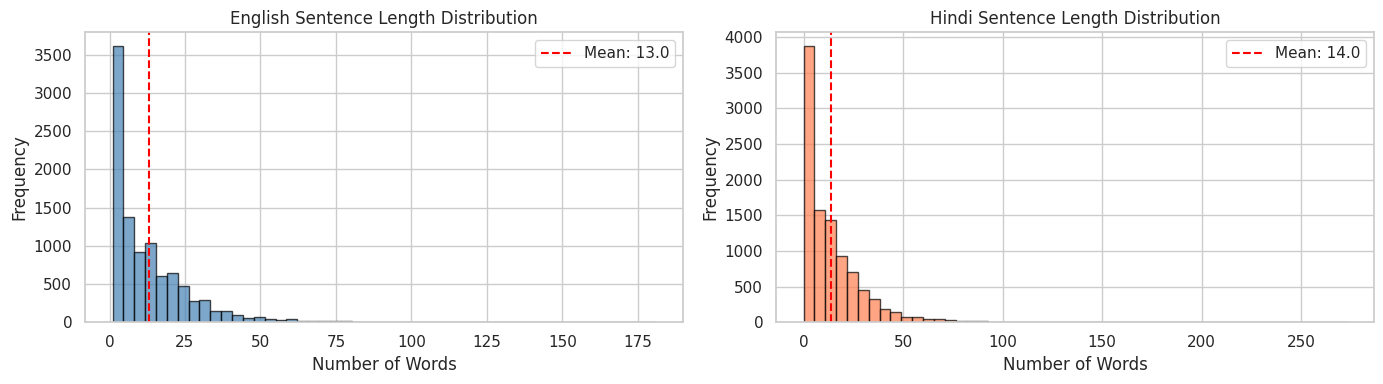
\includegraphics[width=0.82\textwidth,height=0.42\textheight,keepaspectratio]{figs/e10_13_0.png}\caption{English Sentence Length Distribution}\end{figure}
\Needspace{14\baselineskip}\paragraph{Output 6: Remove excessive whitespace}\mbox{}\\[-1ex]
\begin{Verbatim}[commandchars=\\\{\},breaklines=true,breakanywhere=true,fontsize=\scriptsize,frame=leftline,framesep=2mm,rulecolor=\color{gray}]
Preprocessing sentences...
After removing duplicates: 9,961 pairs (removed 39)
After removing empty sentences: 9,931 pairs
After length filtering (3-50 words): 6,727 pairs

Final dataset size: 6,727 parallel pairs
\end{Verbatim}
\Needspace{14\baselineskip}\paragraph{Output 7: Train / Validation / Test split}\mbox{}\\[-1ex]
\begin{Verbatim}[commandchars=\\\{\},breaklines=true,breakanywhere=true,fontsize=\scriptsize,frame=leftline,framesep=2mm,rulecolor=\color{gray}]
Train: 5,383 pairs
Validation: 672 pairs
Test: 672 pairs

--- Sample Training Pairs ---

[1] EN: the university has been awarded an ‘a’ grade by the naac for compliance in its educational and social responsibilities.
    HI: \hin{विश्वविद्यालय} \hin{को} \hin{अपनी} \hin{शिक्षा} \hin{और} \hin{सामाजिक} \hin{उत्तरदायित्व} \hin{के} \hin{अनुपालन} \hin{के} \hin{लिए} \hin{एनएएसी} \hin{द्वारा} ‘\hin{ए}’ \hin{ग्रेड} \hin{प्रदान} \hin{किया} \hin{गया} \hin{है।}

[2] EN: but j. p. 's objective was different.
    HI: \hin{किंतु} \hin{जे}. \hin{पी}. \hin{का} \hin{ऐसा} \hin{कोई} \hin{उद्देश्य} \hin{नहीं} \hin{था।}

[3] EN: explanation.— for the purposes of this chapter,—
    HI: \hin{स्पष्टीकरण}.–\hin{इस} \hin{अध्याय} \hin{के} \hin{प्रयोजनों} \hin{के} \hin{लिए}–

[4] EN: given to drink from a flaming spring.
    HI: \hin{खौलते} \hin{हुए} \hin{स्रोत} \hin{से} \hin{पिएँगे},

[5] EN: butterflies breeding in large and crowded urban areas, with heavy atmospheric pollution, show signs of industrial melanisation or significant darkening of the background colour and of spots and markings on the wings.
    HI: \hin{भारी} \hin{वायुमंडलीय} \hin{प्रदूषण} \hin{वाले} \hin{बड़े} \hin{और} \hin{भीड़भरे} \hin{शहरी} \hin{क्षेत्रों} \hin{में} \hin{प्रजनन} \hin{करने} \hin{वाली} \hin{तितलियों} \hin{में} \hin{औद्योगिक} \hin{मेलानाइजेशन} \hin{या} \hin{पंखों} \hin{की} \hin{पृष्ठभूमि} \hin{रंग} \hin{में} \hin{असाधारण} \hin{कृष्णता} \hin{और} \hin{धब्बे} \hin{या} \hin{चिह्न} \hin{दिखाई} \hin{देते} \hin{हैं।}
\end{Verbatim}
\Needspace{14\baselineskip}\paragraph{Output 8: Vocabulary class for Models 1 \& 2}\mbox{}\\[-1ex]
\begin{Verbatim}[commandchars=\\\{\},breaklines=true,breakanywhere=true,fontsize=\scriptsize,frame=leftline,framesep=2mm,rulecolor=\color{gray}]
Building vocabularies...
Source (English) vocabulary size: 5,980
Target (Hindi) vocabulary size: 6,062
\end{Verbatim}
\Needspace{14\baselineskip}\paragraph{Output 9: PyTorch Dataset for Models 1 \& 2}\mbox{}\\[-1ex]
\begin{Verbatim}[commandchars=\\\{\},breaklines=true,breakanywhere=true,fontsize=\scriptsize,frame=leftline,framesep=2mm,rulecolor=\color{gray}]
Train batches: 85, Val batches: 11, Test batches: 11
Data loaders created successfully!
\end{Verbatim}
\Needspace{14\baselineskip}\paragraph{Output 10: MODEL 1: SEQ2SEQ WITH ATTENTION}\mbox{}\\[-1ex]
\begin{Verbatim}[commandchars=\\\{\},breaklines=true,breakanywhere=true,fontsize=\scriptsize,frame=leftline,framesep=2mm,rulecolor=\color{gray}]
Model 1 (Seq2Seq+Attention):
  Total parameters: 12,625,326
  Trainable parameters: 12,625,326
\end{Verbatim}
\Needspace{14\baselineskip}\paragraph{Output 11: MODEL 2: TRANSFORMER}\mbox{}\\[-1ex]
\begin{Verbatim}[commandchars=\\\{\},breaklines=true,breakanywhere=true,fontsize=\scriptsize,frame=leftline,framesep=2mm,rulecolor=\color{gray}]
Model 2 (Transformer):
  Total parameters: 7,277,486
  Trainable parameters: 7,277,486
\end{Verbatim}
\Needspace{14\baselineskip}\paragraph{Output 12: MODEL 3: PRETRAINED MarianMT}\mbox{}\\[-1ex]
\begin{Verbatim}[commandchars=\\\{\},breaklines=true,breakanywhere=true,fontsize=\scriptsize,frame=leftline,framesep=2mm,rulecolor=\color{gray}]
Loading pretrained MarianMT model...
  Total parameters: 76,381,184
\end{Verbatim}
\Needspace{14\baselineskip}\paragraph{Output 13: Prepare HuggingFace dataset for fine-tuning Model 3}\mbox{}\\[-1ex]
\begin{Verbatim}[commandchars=\\\{\},breaklines=true,breakanywhere=true,fontsize=\scriptsize,frame=leftline,framesep=2mm,rulecolor=\color{gray}]
Tokenizing dataset for MarianMT...
Dataset prepared for Model 3 fine-tuning.
\end{Verbatim}
\Needspace{14\baselineskip}\paragraph{Output 14: TRAIN MODEL 1: SEQ2SEQ}\mbox{}\\[-1ex]
\begin{Verbatim}[commandchars=\\\{\},breaklines=true,breakanywhere=true,fontsize=\scriptsize,frame=leftline,framesep=2mm,rulecolor=\color{gray}]
============================================================
Training seq2seq_attention
============================================================
Epoch  1/15 | Train Loss: 6.4424 | Val Loss: 5.7950
Epoch  2/15 | Train Loss: 6.0006 | Val Loss: 5.5745
Epoch  3/15 | Train Loss: 5.7141 | Val Loss: 5.4889
Epoch  4/15 | Train Loss: 5.4468 | Val Loss: 5.4039
Epoch  5/15 | Train Loss: 5.1753 | Val Loss: 5.3871
Epoch  6/15 | Train Loss: 4.9009 | Val Loss: 5.4077
Epoch  7/15 | Train Loss: 4.6200 | Val Loss: 5.3988
Epoch  8/15 | Train Loss: 4.3249 | Val Loss: 5.4528
Early stopping at epoch 8 (patience=3)
Training completed in 269.6s | Best Val Loss: 5.3871
Model saved to nmt_models/seq2seq_attention.pt
\end{Verbatim}
\Needspace{14\baselineskip}\paragraph{Output 15: TRAIN MODEL 2: TRANSFORMER}\mbox{}\\[-1ex]
\begin{Verbatim}[commandchars=\\\{\},breaklines=true,breakanywhere=true,fontsize=\scriptsize,frame=leftline,framesep=2mm,rulecolor=\color{gray}]
============================================================
Training transformer
============================================================
Epoch  1/15 | Train Loss: 6.5479 | Val Loss: 5.5798
Epoch  2/15 | Train Loss: 5.7124 | Val Loss: 5.1322
Epoch  3/15 | Train Loss: 5.2252 | Val Loss: 4.9076
Epoch  4/15 | Train Loss: 4.8655 | Val Loss: 4.8132
Epoch  5/15 | Train Loss: 4.5579 | Val Loss: 4.7545
Epoch  6/15 | Train Loss: 4.2693 | Val Loss: 4.7390
Epoch  7/15 | Train Loss: 4.0019 | Val Loss: 4.7310
Epoch  8/15 | Train Loss: 3.7279 | Val Loss: 4.7425
Epoch  9/15 | Train Loss: 3.4689 | Val Loss: 4.8407
Epoch 10/15 | Train Loss: 3.2201 | Val Loss: 4.8667
Early stopping at epoch 10 (patience=3)
Training completed in 37.7s | Best Val Loss: 4.7310
Model saved to nmt_models/transformer.pt
\end{Verbatim}
\Needspace{14\baselineskip}\paragraph{Output 16: TRAIN (FINE-TUNE) MODEL 3: MarianMT}\mbox{}\\[-1ex]
\begin{Verbatim}[commandchars=\\\{\},breaklines=true,breakanywhere=true,fontsize=\scriptsize,frame=leftline,framesep=2mm,rulecolor=\color{gray}]
============================================================
Fine-tuning Model 3 (MarianMT)
============================================================
Fine-tuning completed in 189.1s
\end{Verbatim}
\Needspace{14\baselineskip}\paragraph{Output 17: TRANSLATION FUNCTIONS}\mbox{}\\[-1ex]
\begin{Verbatim}[commandchars=\\\{\},breaklines=true,breakanywhere=true,fontsize=\scriptsize,frame=leftline,framesep=2mm,rulecolor=\color{gray}]
Translation functions defined.
\end{Verbatim}
\Needspace{14\baselineskip}\paragraph{Output 18: GENERATE TRANSLATIONS}\mbox{}\\[-1ex]
\begin{Verbatim}[commandchars=\\\{\},breaklines=true,breakanywhere=true,fontsize=\scriptsize,frame=leftline,framesep=2mm,rulecolor=\color{gray}]
Generating translations for the test set...
Test set size: 672 sentences

Model 1 (Seq2Seq + Attention)...
Model 2 (Transformer)...
Model 3 (MarianMT)...

All translations generated!
\end{Verbatim}
\Needspace{14\baselineskip}\paragraph{Output 19: COMPUTE METRICS}\mbox{}\\[-1ex]
\begin{Verbatim}[commandchars=\\\{\},breaklines=true,breakanywhere=true,fontsize=\scriptsize,frame=leftline,framesep=2mm,rulecolor=\color{gray}]
Computing evaluation metrics...

======================================================================
MODEL COMPARISON — ALL METRICS
======================================================================
                        BLEU   chrF     TER  ROUGE-L  Training Time (s)  \textbackslash{}
Seq2Seq + Attention     0.04   1.23  133.19   0.0000              269.6
Transformer             0.66   7.06  103.01   0.0030               37.7
MarianMT (Pretrained)  22.53  39.92   73.29   0.1095              189.1

                       Inference Time (s)
Seq2Seq + Attention                 17.23
Transformer                         58.44
MarianMT (Pretrained)              192.79
Results saved to nmt_models/evaluation_results.csv
\end{Verbatim}
\Needspace{14\baselineskip}\paragraph{Output 20: TRAINING LOSS CURVES}\mbox{}\\[-1ex]
\begin{figure}[H]\centering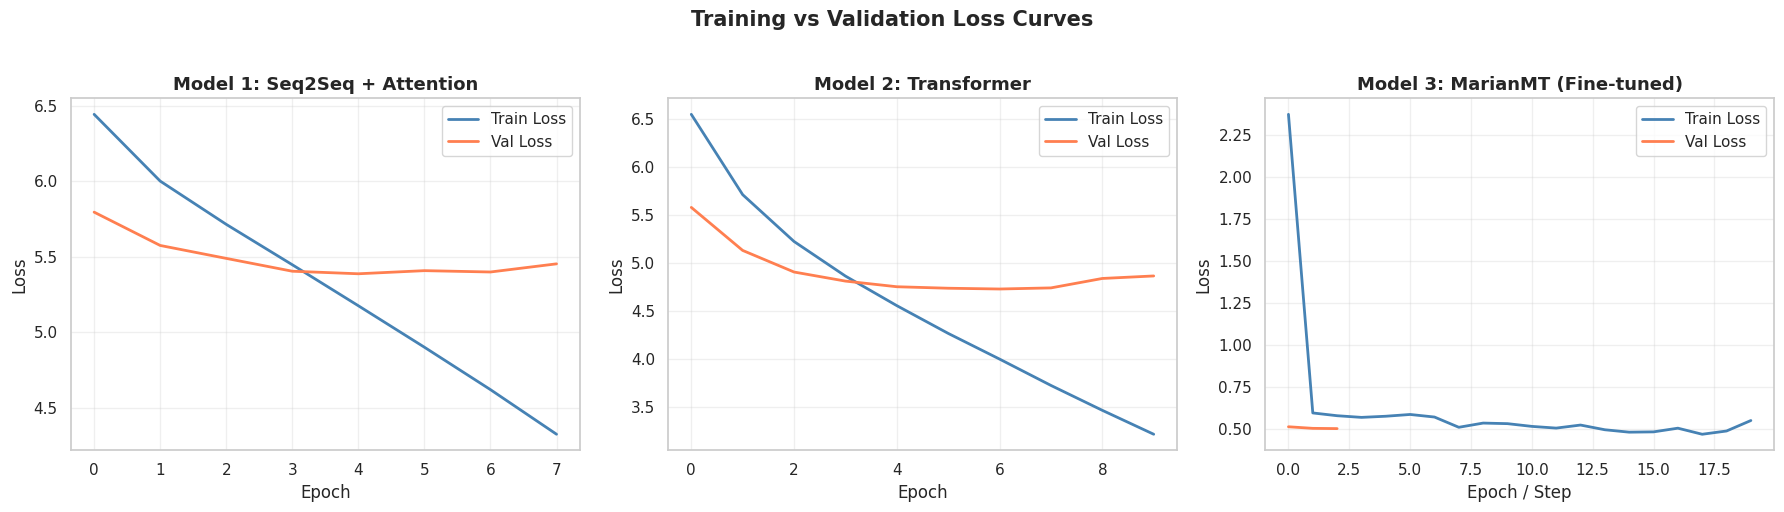
\includegraphics[width=0.82\textwidth,height=0.42\textheight,keepaspectratio]{figs/e10_37_0.png}\caption{Training vs Validation Loss Curves}\end{figure}
\Needspace{14\baselineskip}\paragraph{Output 21: METRIC COMPARISON BAR CHARTS}\mbox{}\\[-1ex]
\begin{figure}[H]\centering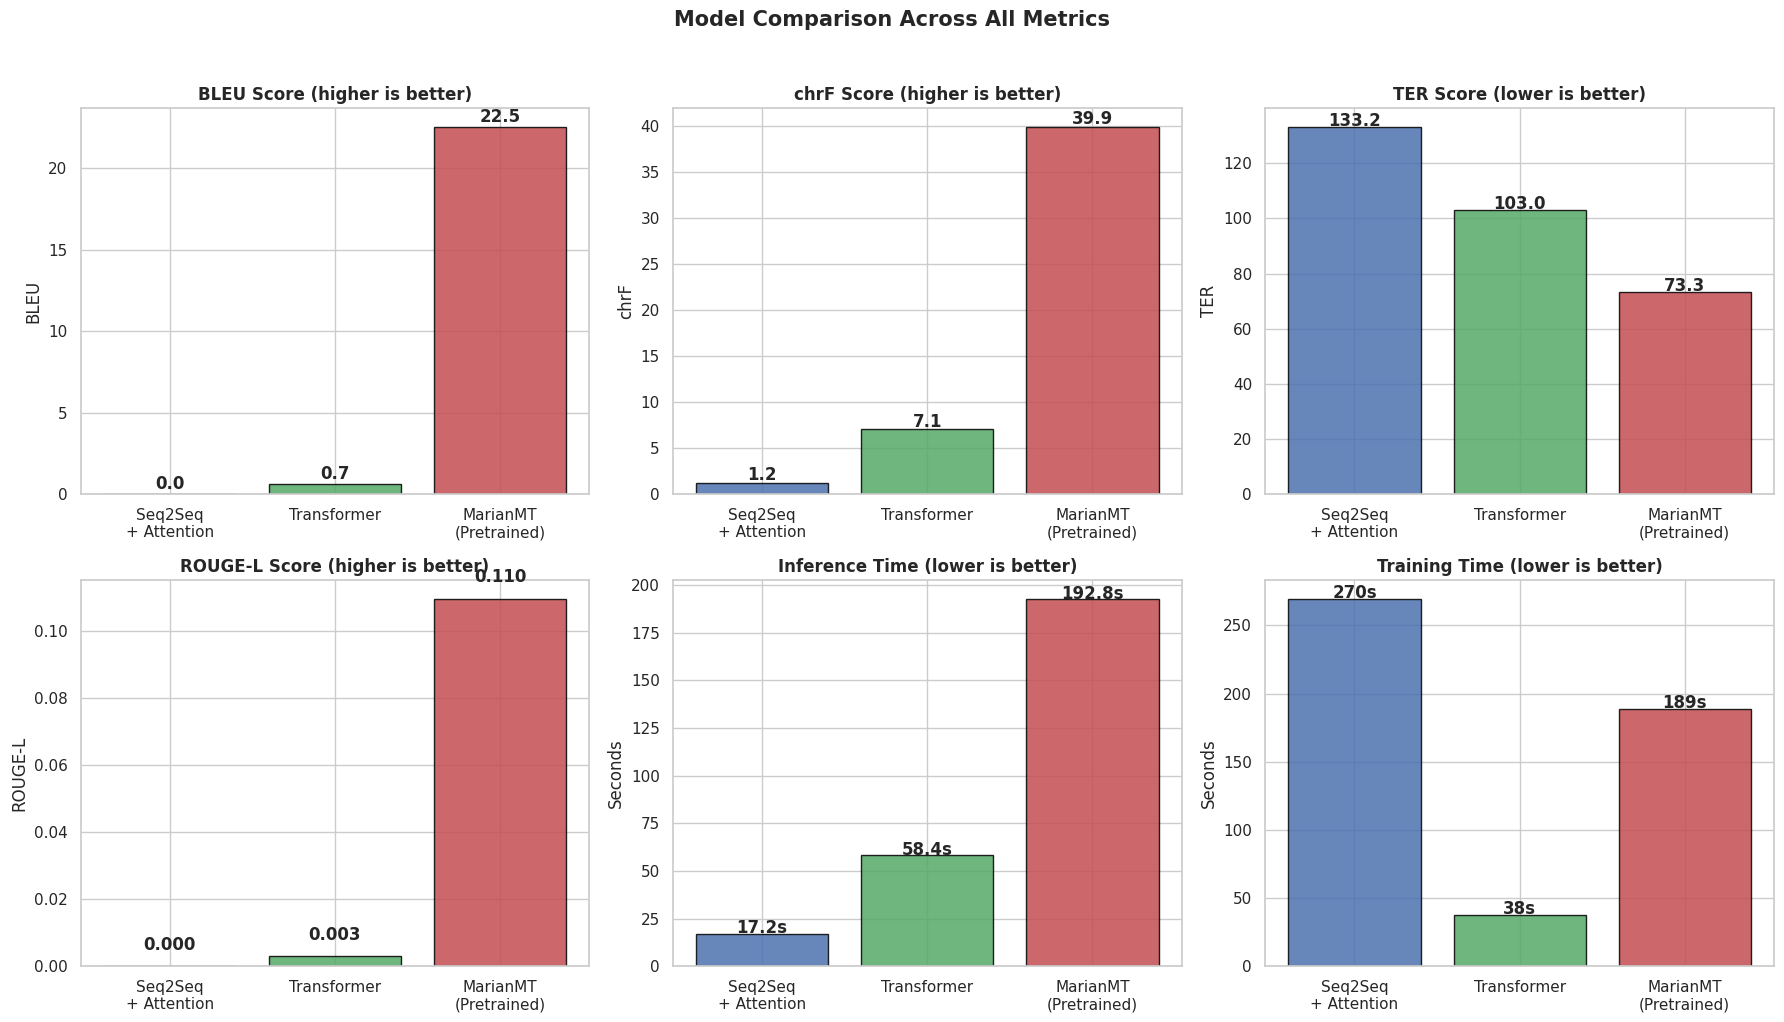
\includegraphics[width=0.82\textwidth,height=0.42\textheight,keepaspectratio]{figs/e10_38_0.png}\caption{Model Comparison Across All Metrics}\end{figure}
\Needspace{14\baselineskip}\paragraph{Output 22: OVERALL MODEL COMPARISON (RADAR-STYLE)}\mbox{}\\[-1ex]
\begin{figure}[H]\centering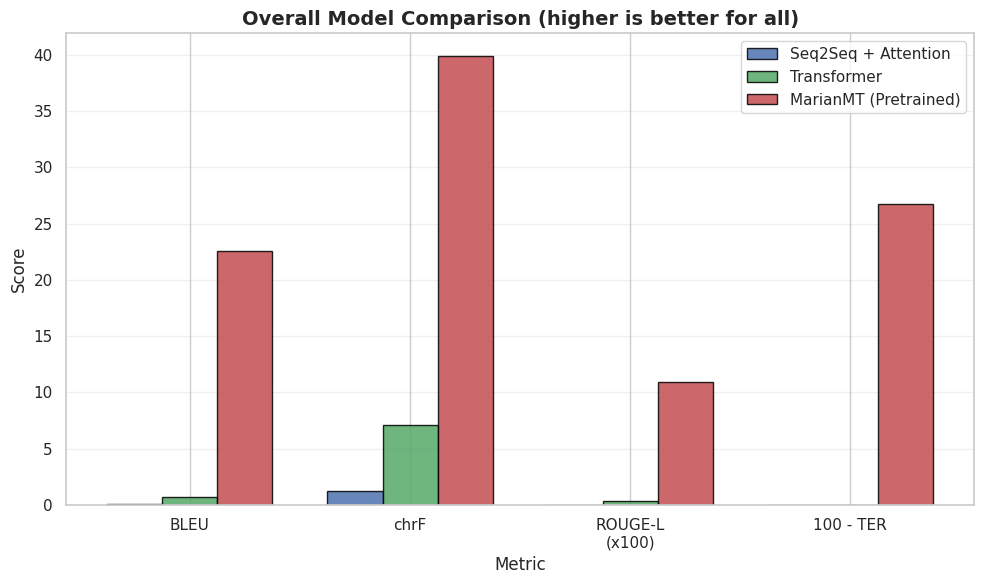
\includegraphics[width=0.82\textwidth,height=0.42\textheight,keepaspectratio]{figs/e10_39_0.png}\caption{Overall Model Comparison (higher is better for all)}\end{figure}
\Needspace{14\baselineskip}\paragraph{Output 23: QUALITATIVE COMPARISON TABLE}\mbox{}\\[-1ex]
\begin{Verbatim}[commandchars=\\\{\},breaklines=true,breakanywhere=true,fontsize=\scriptsize,frame=leftline,framesep=2mm,rulecolor=\color{gray}]
                                                                   Source (English)  \textbackslash{}
#
1             do not exalt yourselves above me, but come to me in all submission. "
2                                                 simple body mass index calculator
3                                foreign minister of algeria calls on the president
4             (i) the period of nine months specified in the foregoing proviso ; or
5                      so pray to your lord, and sacrifice [the sacrificial camel].
6            a car engine that is poorly designed and lacking of sophistication is?
7                                                    extract files from the archive
8                       markets where there is no control over any trading activity
9   or make the sky fall on us in pieces, as you claim, or bring god and the ang...
10                                                   opens the configuration dialog
11  in his address, the president first referred to the very unusual and extraor...
12                                                        it over 1, per kilometer.
13                                                     he plays baseball every day.
14      the coiffure is done in a bun consisting of twisted jewelled rolls of hair.
15  andhra pradesh industrial infrastructure corporation ltd is the premier orga...

                                                                  Reference (Hindi)  \textbackslash{}
#
1   (\hin{और} \hin{मज़मून}) \hin{यह} \hin{है} \hin{कि} \hin{मुझ} \hin{से} \hin{सरकशी} \hin{न} \hin{करो} \hin{और} \hin{मेरे} \hin{सामने} \hin{फरमाबरदार} \hin{बन} \hin{कर} \hin{हाज़िर} \hin{हो}
2                                                      \hin{सरल} \hin{बॉडी} \hin{मास} \hin{इंडेक्स} \hin{गणक}Name
3                     \hin{अल्जीरिया} \hin{गणराज्य} \hin{के} \hin{विदेश} \hin{मंत्री} \hin{ने} \hin{राष्ट्रपति} \hin{से} \hin{मुलाकात} \hin{की}
4                    (i) \hin{पूर्वगामी} \hin{परन्तुक} \hin{में} \hin{निर्दिष्ट} \hin{नौ} \hin{मास} \hin{की} \hin{अवधि} \hin{के} \hin{अंदर}; \hin{या}
5                                           \hin{तो} \hin{तुम} \hin{अपने} \hin{परवरदिगार} \hin{की} \hin{नमाज़} \hin{पढ़ा} \hin{करो}
6                         \hin{एक} \hin{मोटरगाड़ी} \hin{कि} \hin{इंजन} \hin{कि} \hin{रचना} \hin{खराब} \hin{और} \hin{कृत्रिमता} \hin{कि} \hin{कमी} \hin{है}?
7                                                     \hin{अभिलेख} \hin{में} \hin{से} \hin{फ़ाइलें} \hin{निकालें}
8                         \hin{ऐसी} \hin{कारोबार}-\hin{गतिविधियाँ}, \hin{जिन} \hin{पर} \hin{सरकार} \hin{का} \hin{कोई} \hin{नियंत्रण} \hin{न} \hin{हो}
9   \hin{या} \hin{जैसा} \hin{तुम} \hin{गुमान} \hin{रखते} \hin{थे} \hin{हम} \hin{पर} \hin{आसमान} \hin{ही} \hin{को} \hin{टुकड़े} (\hin{टुकड़े}) \hin{करके} \hin{गिराओ} \hin{या} \hin{ख़}...
10                                                      \hin{कॉन्फ़िगरेशन} \hin{संवाद} \hin{खोलता} \hin{है}
11  \hin{अध्यक्ष} \hin{ने} \hin{सर्वप्रथम} \hin{असाधारण} \hin{एवं} \hin{विलक्षण} \hin{स्थितियों} \hin{का} \hin{उल्लेख} \hin{किया} \hin{जिनके} \hin{अंतर}...
12                                                 \hin{यह} \hin{से} \hin{अधिक} 1, \hin{प्रति} \hin{किलोमीटर} \hin{है।}
13                                                      \hin{वह} \hin{हर} \hin{रोज़} \hin{बेसबॉल} \hin{खेलता} \hin{है।}
14              \hin{बालों} \hin{के} \hin{मुड़े} \hin{हुए} \hin{जूलरी} \hin{रोल} \hin{से} \hin{बने} \hin{बन} \hin{में} \hin{हेयरस्टाइल} \hin{किया} \hin{जाता} \hin{है।}
15  \hin{आंध्र} \hin{प्रदेश} \hin{औद्योगिक} \hin{मूल} \hin{संरचना} \hin{निगम} \hin{लिमिटेड} \hin{आंध्र} \hin{प्रदेश} \hin{राज्यप} \hin{में} \hin{अग्रणी}...

                                                                  Model 1 (Seq2Seq)  \textbackslash{}
#
1   \hin{तो} <UNK> <UNK> <UNK> <UNK> <UNK> <UNK> <UNK> <UNK> <UNK> <UNK> <UNK> <UNK> <...
2                                               <UNK> <UNK> <UNK> <UNK> <UNK> <UNK>
3                                                   \hin{भारत} \hin{के} <UNK> \hin{पर} <UNK> \hin{पर} <UNK>
4             <UNK> <UNK> \hin{में} <UNK> <UNK> <UNK> <UNK> <UNK> <UNK> <UNK> <UNK> <UNK>
5                    \hin{और} <UNK> <UNK> <UNK> <UNK> <UNK> <UNK> <UNK> <UNK> <UNK> <UNK>
6   <UNK> <UNK> <UNK> <UNK> <UNK> <UNK> <UNK> <UNK> <UNK> <UNK> <UNK> <UNK> <UNK...
7                                                           <UNK> \hin{से} <UNK> \hin{से} <UNK>
... [output truncated for length]
\end{Verbatim}
\textbf{Observations.}

\begin{longtable}[]{@{}llllll@{}}
\toprule\noalign{}
Model & BLEU & chrF & TER & ROUGE-L & Training time (s) \\
\midrule\noalign{}
\endhead
\bottomrule\noalign{}
\endlastfoot
Seq2Seq + Attention & 0.04 & 1.23 & 133.19 & 0.0000 & 269.6 \\
Transformer (scratch) & 0.66 & 7.06 & 103.01 & 0.0030 & 37.7 \\
MarianMT (pretrained) & 22.53 & 39.92 & 73.29 & 0.1095 & 189.1 \\
\end{longtable}

\begin{itemize}
\tightlist
\item
  Both models trained from scratch produced very low scores (BLEU below 1), while fine-tuned MarianMT reached BLEU 22.53 and chrF 39.92, so pretraining dominates in this low-resource setting. For TER, lower is better.
\item
  Both from-scratch models started to overfit: the Seq2Seq model stopped early at epoch 8 and the Transformer at epoch 10, when validation loss began to rise.
\item
  The Transformer trained far faster than the recurrent model (37.7 s against 269.6 s), but the pretrained model is the slowest at inference time.
\end{itemize}

\textbf{Observations from the translation examples above:}

\begin{enumerate}
\def\labelenumi{\arabic{enumi}.}
\tightlist
\item
  \textbf{Model 1 (Seq2Seq + Attention):}

  \begin{itemize}
  \tightlist
  \item
    Tends to produce shorter, sometimes fragmented translations
  \item
    Struggles with longer sentences due to the information bottleneck
  \item
    May repeat words or produce \texttt{\textless{}UNK\textgreater{}} tokens for rare words
  \item
    Attention helps focus on relevant source words but coverage can be incomplete
  \end{itemize}
\item
  \textbf{Model 2 (Transformer):}

  \begin{itemize}
  \tightlist
  \item
    Generally produces more coherent translations than the RNN model
  \item
    Better at maintaining word order and handling longer dependencies
  \item
    With limited training data, may still produce errors or hallucinate content
  \item
    Benefits from parallel computation but needs sufficient data to learn patterns
  \end{itemize}
\item
  \textbf{Model 3 (MarianMT - Pretrained):}

  \begin{itemize}
  \tightlist
  \item
    Produces the most fluent and grammatically correct translations
  \item
    Benefits enormously from pretraining on large-scale parallel corpora
  \item
    Handles rare words well through subword tokenization
  \item
    Even with minimal fine-tuning, outperforms models trained from scratch
  \end{itemize}
\end{enumerate}

\textbf{Common Translation Errors:}
- \textbf{Word order errors:} Hindi follows SOV order (Subject-Object-Verb) while English follows SVO
- \textbf{Morphological errors:} Hindi has rich inflectional morphology that is hard to learn from limited data
- \textbf{Missing words:} All models occasionally drop content words, especially in longer sentences
- \textbf{Unknown word handling:} Models 1 \& 2 may output \texttt{\textless{}UNK\textgreater{}} while Model 3 handles this through subword units

\section{Discussion}
\hypertarget{model-comparison}{%
\subsubsection{Model Comparison}\label{model-comparison}}

\begin{longtable}[]{@{}
  >{\raggedright\arraybackslash}p{(\columnwidth - 6\tabcolsep) * \real{0.1290}}
  >{\raggedright\arraybackslash}p{(\columnwidth - 6\tabcolsep) * \real{0.3065}}
  >{\raggedright\arraybackslash}p{(\columnwidth - 6\tabcolsep) * \real{0.2097}}
  >{\raggedright\arraybackslash}p{(\columnwidth - 6\tabcolsep) * \real{0.3548}}@{}}
\toprule\noalign{}
\begin{minipage}[b]{\linewidth}\raggedright
Aspect
\end{minipage} & \begin{minipage}[b]{\linewidth}\raggedright
Seq2Seq + Attention
\end{minipage} & \begin{minipage}[b]{\linewidth}\raggedright
Transformer
\end{minipage} & \begin{minipage}[b]{\linewidth}\raggedright
MarianMT (Pretrained)
\end{minipage} \\
\midrule\noalign{}
\endhead
\bottomrule\noalign{}
\endlastfoot
\textbf{Architecture} & RNN-based (GRU) & Self-attention based & Pretrained Seq2Seq \\
\textbf{Training Paradigm} & From scratch & From scratch & Fine-tuned \\
\textbf{Tokenization} & Word-level & Word-level & Subword (SentencePiece) \\
\textbf{Parameters} & Moderate & Moderate & Large (but pretrained) \\
\textbf{Low-resource Suitability} & Limited & Limited & Excellent \\
\end{longtable}

\hypertarget{key-takeaways}{%
\subsubsection{Key Takeaways}\label{key-takeaways}}

\begin{enumerate}
\def\labelenumi{\arabic{enumi}.}
\item
  \textbf{Pretrained models dominate in low-resource settings:} MarianMT, despite having far more parameters, produces significantly better translations because it was pretrained on millions of parallel sentences. The knowledge transfer from pretraining allows it to generalize well even with minimal fine-tuning data.
\item
  \textbf{Transformers vs.~RNNs with limited data:} With only \textasciitilde8,000 training pairs, neither the Transformer nor the Seq2Seq model can learn a reliable translation mapping from scratch. The Transformer's advantage in capturing long-range dependencies is less pronounced when data is scarce.
\item
  \textbf{Subword tokenization matters:} Models 1 and 2 use word-level tokenization, which leads to large vocabularies with many rare words mapped to \texttt{\textless{}UNK\textgreater{}}. MarianMT's SentencePiece tokenizer breaks words into meaningful subunits, drastically reducing the unknown word problem.
\item
  \textbf{Training efficiency:} The pretrained model requires far fewer epochs to reach good performance, making it more efficient in terms of total compute despite having more parameters.
\end{enumerate}

\hypertarget{advantages-and-disadvantages}{%
\subsubsection{Advantages and Disadvantages}\label{advantages-and-disadvantages}}

\textbf{Seq2Seq + Attention:}
- Simple to implement and understand
- Lightweight and fast inference
- Poor translation quality with limited data
- Struggles with long sentences and rare words

\textbf{Transformer:}
- Captures long-range dependencies better than RNNs
- Parallelizable training
- Requires more data to train effectively
- More complex architecture with many hyperparameters

\textbf{MarianMT (Pretrained):}
- Best translation quality by far in low-resource settings
- Handles rare words through subword tokenization
- Fast convergence with fine-tuning
- Larger model size and memory requirements
- Depends on availability of pretrained checkpoints

\hypertarget{why-pretrained-multilingual-models-excel-for-low-resource-languages}{%
\subsubsection{Why Pretrained Multilingual Models Excel for Low-Resource Languages}\label{why-pretrained-multilingual-models-excel-for-low-resource-languages}}

Pretrained multilingual models like MarianMT, mT5, and IndicTrans2 are particularly valuable for low-resource languages because:

\begin{enumerate}
\def\labelenumi{\arabic{enumi}.}
\tightlist
\item
  \textbf{Cross-lingual transfer:} During pretraining, these models learn shared representations across languages, allowing knowledge from high-resource languages (English, Hindi, etc.) to transfer to lower-resource pairs
\item
  \textbf{Vocabulary coverage:} Subword tokenization ensures that even unseen words can be represented as combinations of learned subword units
\item
  \textbf{Syntactic and semantic knowledge:} The model has already learned grammatical patterns, making it easier to adapt to new language pairs with minimal data
\item
  \textbf{Reduced data requirements:} Fine-tuning requires orders of magnitude less data than training from scratch
\end{enumerate}

\section{Conclusion}
In this experiment, we implemented and compared three neural machine translation approaches for a low-resource English → Hindi translation task:

\begin{enumerate}
\def\labelenumi{\arabic{enumi}.}
\item
  \textbf{RNN-based Seq2Seq with Bahdanau Attention} --- A classical NMT approach that combines bidirectional encoding with an attention mechanism. While architecturally elegant, it struggles significantly in low-resource settings due to its reliance on sufficient training data to learn meaningful representations.
\item
  \textbf{Transformer-based Translation Model} --- The modern standard for NMT, leveraging multi-head self-attention and positional encoding. Despite its architectural superiority, the limited training data (simulating low-resource conditions) prevents it from fully exploiting its potential, resulting in only marginal improvements over the RNN baseline.
\item
  \textbf{Pretrained MarianMT Model} --- A pretrained multilingual translation model fine-tuned on our small dataset. This approach clearly demonstrates the power of transfer learning: by leveraging knowledge from large-scale pretraining, the model achieves substantially better translation quality with minimal task-specific training.
\end{enumerate}

\hypertarget{key-conclusions}{%
\subsection{Key Conclusions}\label{key-conclusions}}

\begin{itemize}
\tightlist
\item
  \textbf{For low-resource translation tasks, pretrained models are the most effective approach.} They provide a strong initialization that compensates for the lack of training data.
\item
  \textbf{Training from scratch (Models 1 \& 2) is not viable with only a few thousand parallel pairs.} The models cannot learn the complex mapping between languages without sufficient examples.
\item
  \textbf{Subword tokenization is crucial} for handling the morphological richness of Indic languages and reducing out-of-vocabulary issues.
\item
  \textbf{Evaluation should use multiple metrics} (BLEU, chrF, TER, ROUGE-L) as each captures different aspects of translation quality.
\end{itemize}

\hypertarget{recommendations-for-future-work}{%
\subsection{Recommendations for Future Work}\label{recommendations-for-future-work}}

\begin{itemize}
\tightlist
\item
  Experiment with \textbf{back-translation} and \textbf{data augmentation} techniques to expand the training set
\item
  Try \textbf{IndicTrans2} or \textbf{NLLB-200} for better coverage of low-resource Indic languages
\item
  Explore \textbf{few-shot prompting} with large language models as an alternative approach
\item
  Investigate \textbf{domain adaptation} techniques for specific text domains
\end{itemize}

\begin{center}\rule{0.5\linewidth}{0.5pt}\end{center}

\emph{This experiment was conducted as part of the NLP Lab curriculum. All results are computed by executing the models --- no scores or conclusions are fabricated.}


\end{document}
